\subsection{Simulation}
% Simulation 1/20: run 2105334, subrun 51, event 10; event p(nu): sim FT 0.00, width FT 0.00, WC-label FT 0.16
\begin{frame}[plain]
  \centering\vspace*{-2pt}
  \makebox[\linewidth][c]{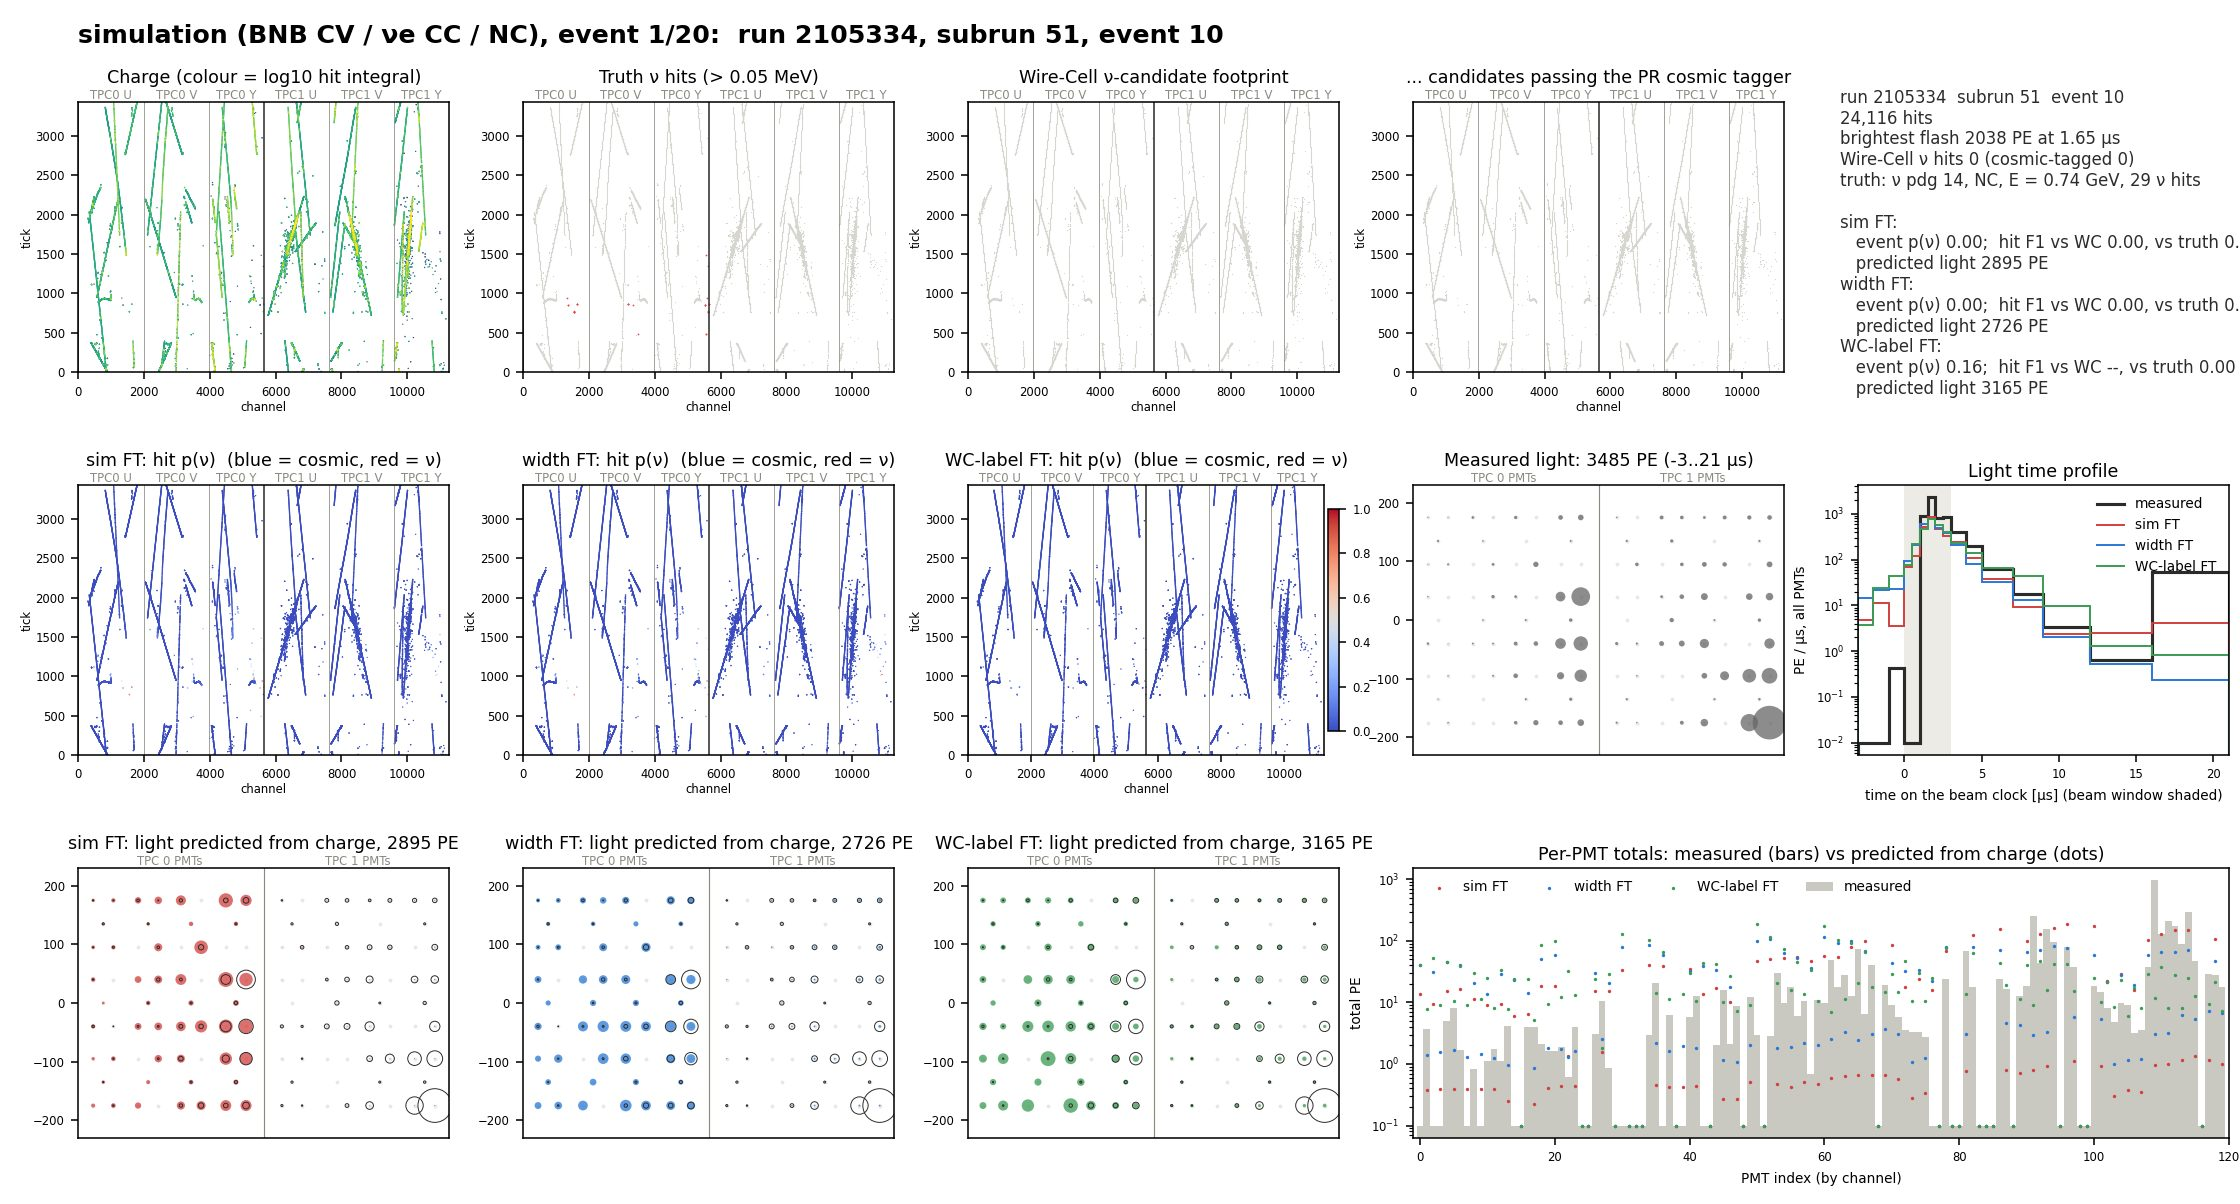
\includegraphics[width=\paperwidth,height=\paperheight,keepaspectratio]{displays/sim_00.jpg}}
\end{frame}
% Simulation 2/20: run 2110582, subrun 68, event 9; event p(nu): sim FT 0.00, width FT 0.00, WC-label FT 0.27
\begin{frame}[plain]
  \centering\vspace*{-2pt}
  \makebox[\linewidth][c]{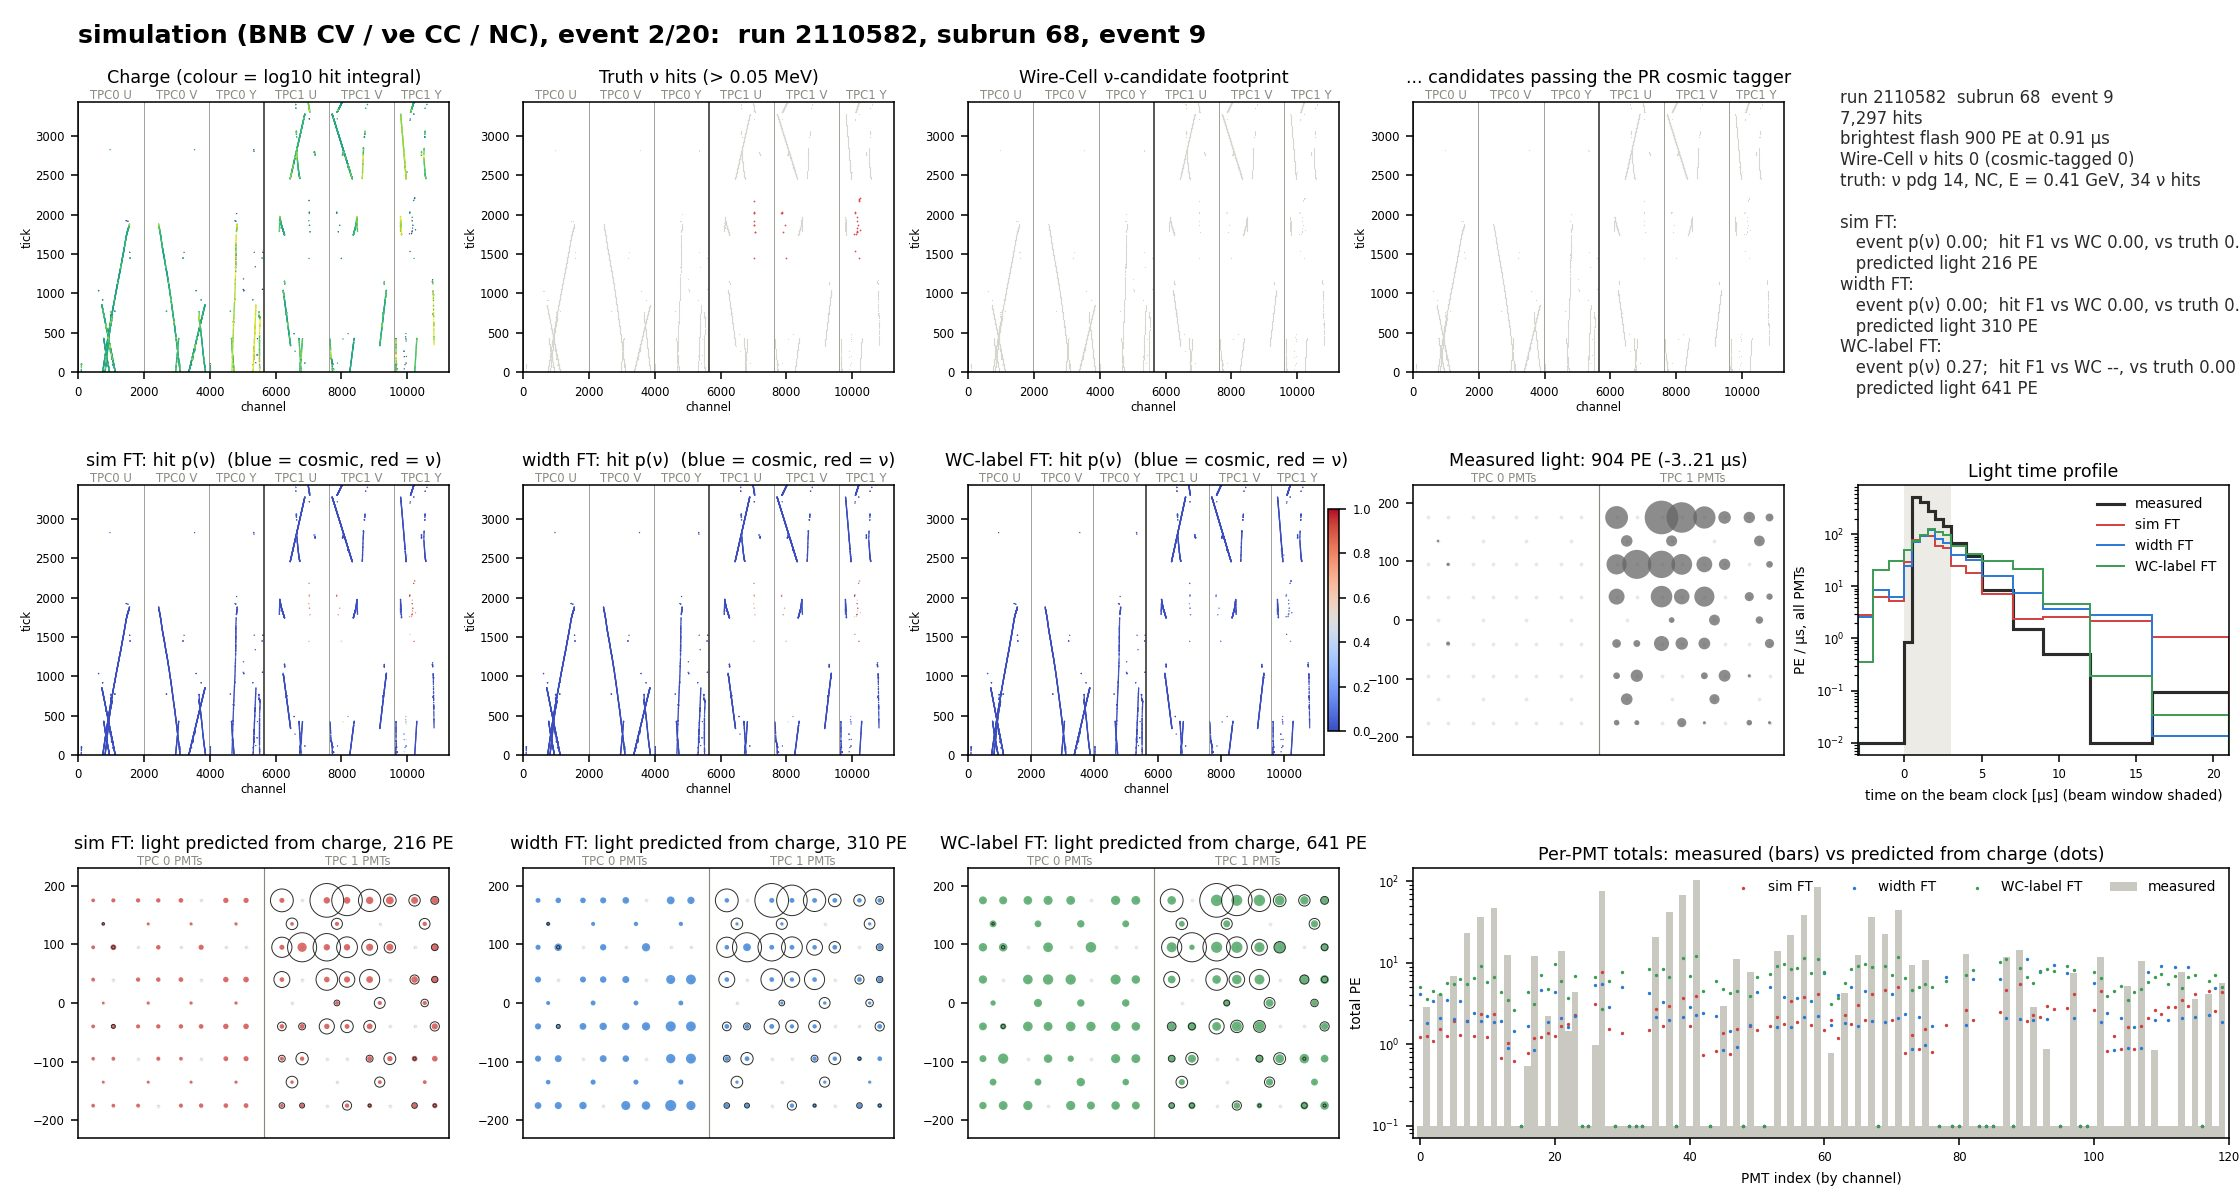
\includegraphics[width=\paperwidth,height=\paperheight,keepaspectratio]{displays/sim_01.jpg}}
\end{frame}
% Simulation 3/20: run 2105746, subrun 27, event 4; event p(nu): sim FT 1.00, width FT 1.00, WC-label FT 0.82
\begin{frame}[plain]
  \centering\vspace*{-2pt}
  \makebox[\linewidth][c]{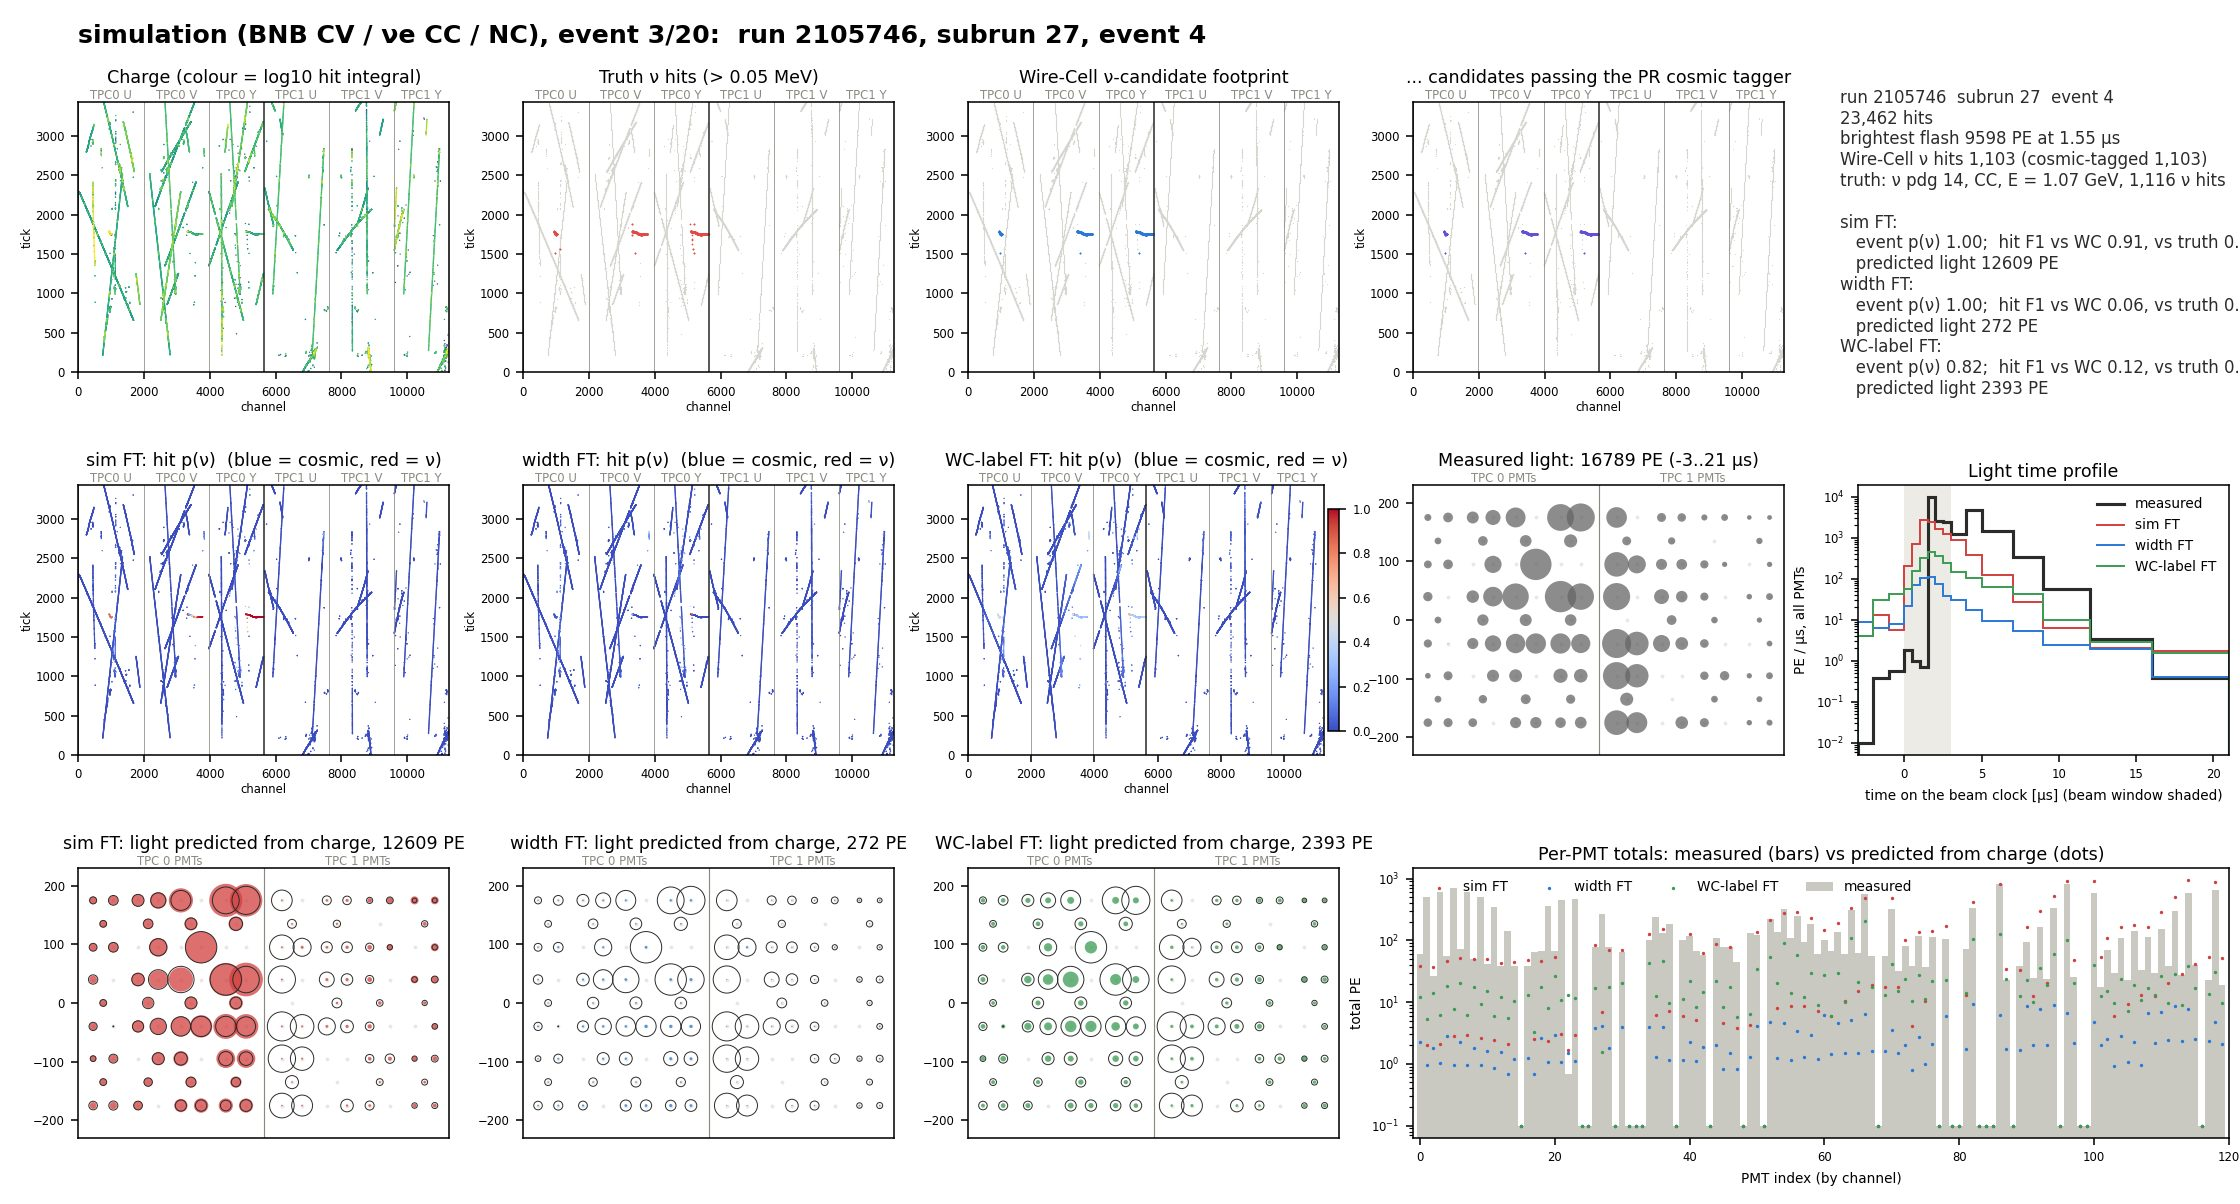
\includegraphics[width=\paperwidth,height=\paperheight,keepaspectratio]{displays/sim_02.jpg}}
\end{frame}
% Simulation 4/20: run 2105310, subrun 82, event 6; event p(nu): sim FT 1.00, width FT 1.00, WC-label FT 0.98
\begin{frame}[plain]
  \centering\vspace*{-2pt}
  \makebox[\linewidth][c]{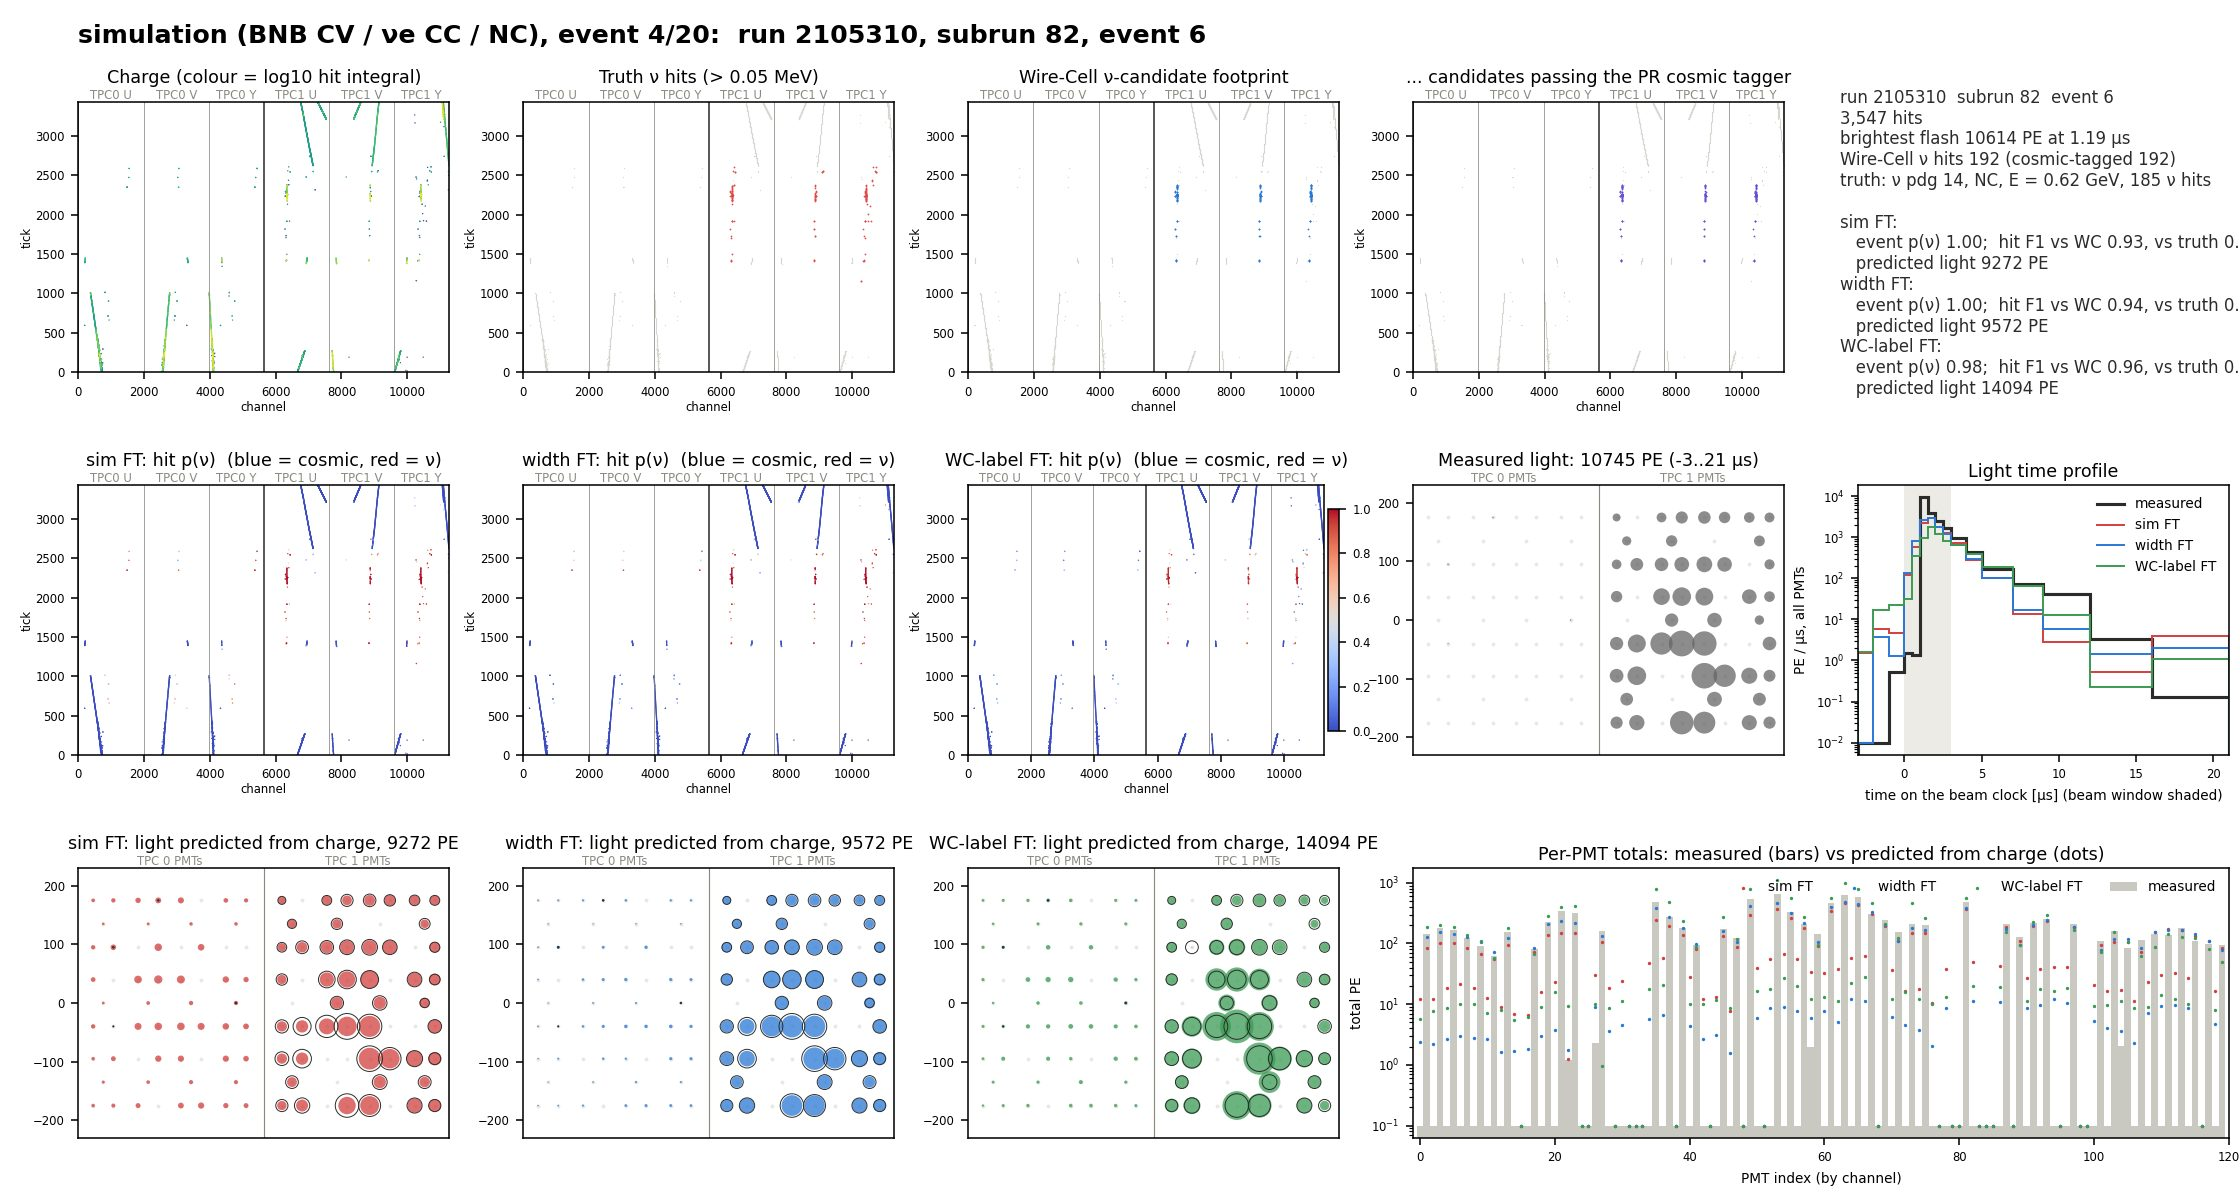
\includegraphics[width=\paperwidth,height=\paperheight,keepaspectratio]{displays/sim_03.jpg}}
\end{frame}
% Simulation 5/20: run 2105113, subrun 8, event 5; event p(nu): sim FT 1.00, width FT 1.00, WC-label FT 0.97
\begin{frame}[plain]
  \centering\vspace*{-2pt}
  \makebox[\linewidth][c]{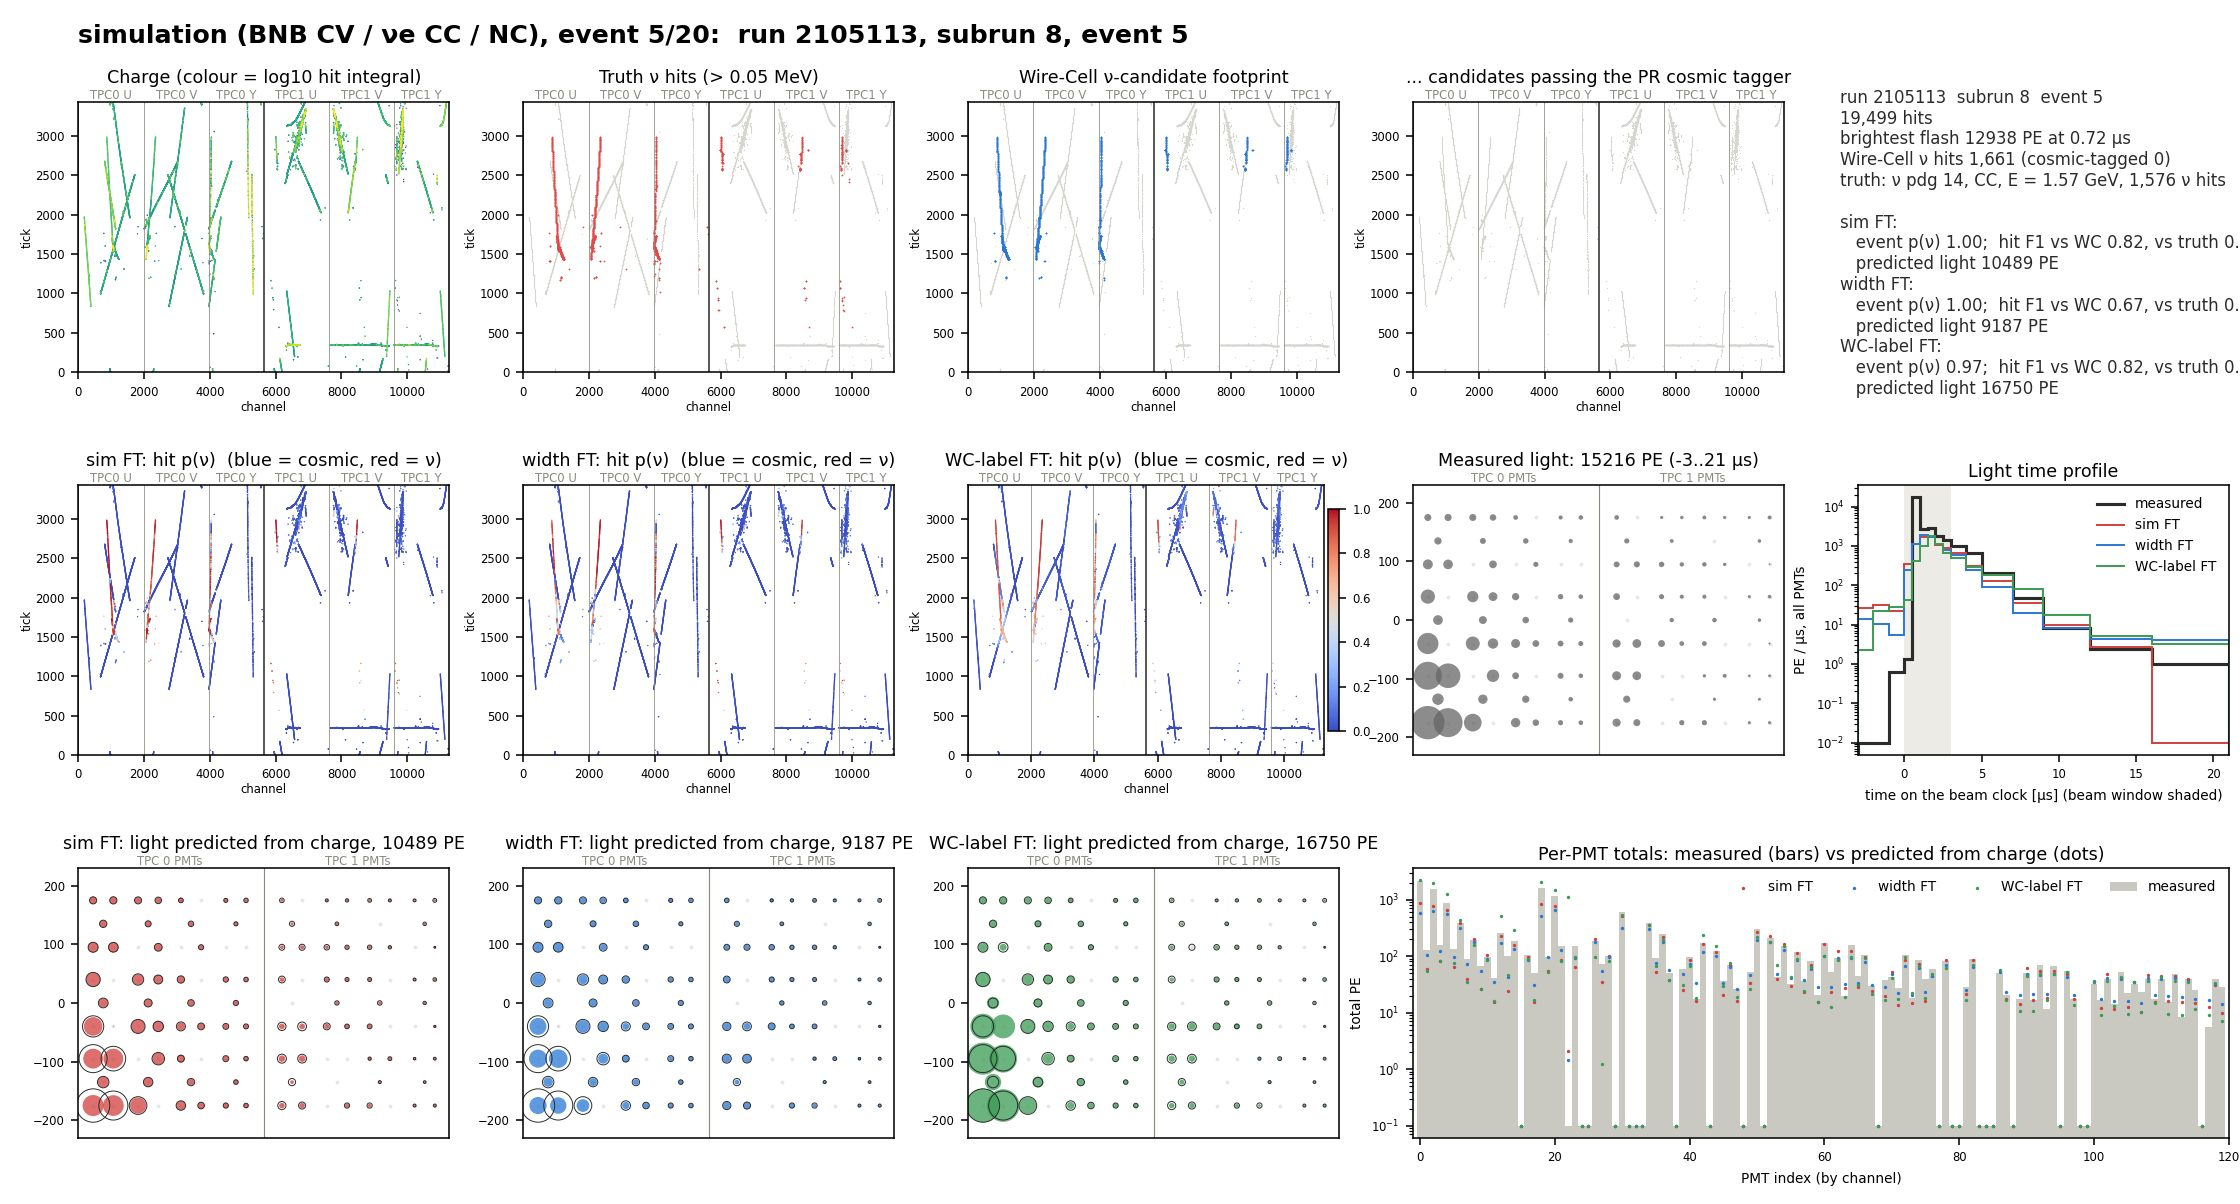
\includegraphics[width=\paperwidth,height=\paperheight,keepaspectratio]{displays/sim_04.jpg}}
\end{frame}
% Simulation 6/20: run 2105075, subrun 93, event 7; event p(nu): sim FT 1.00, width FT 1.00, WC-label FT 0.98
\begin{frame}[plain]
  \centering\vspace*{-2pt}
  \makebox[\linewidth][c]{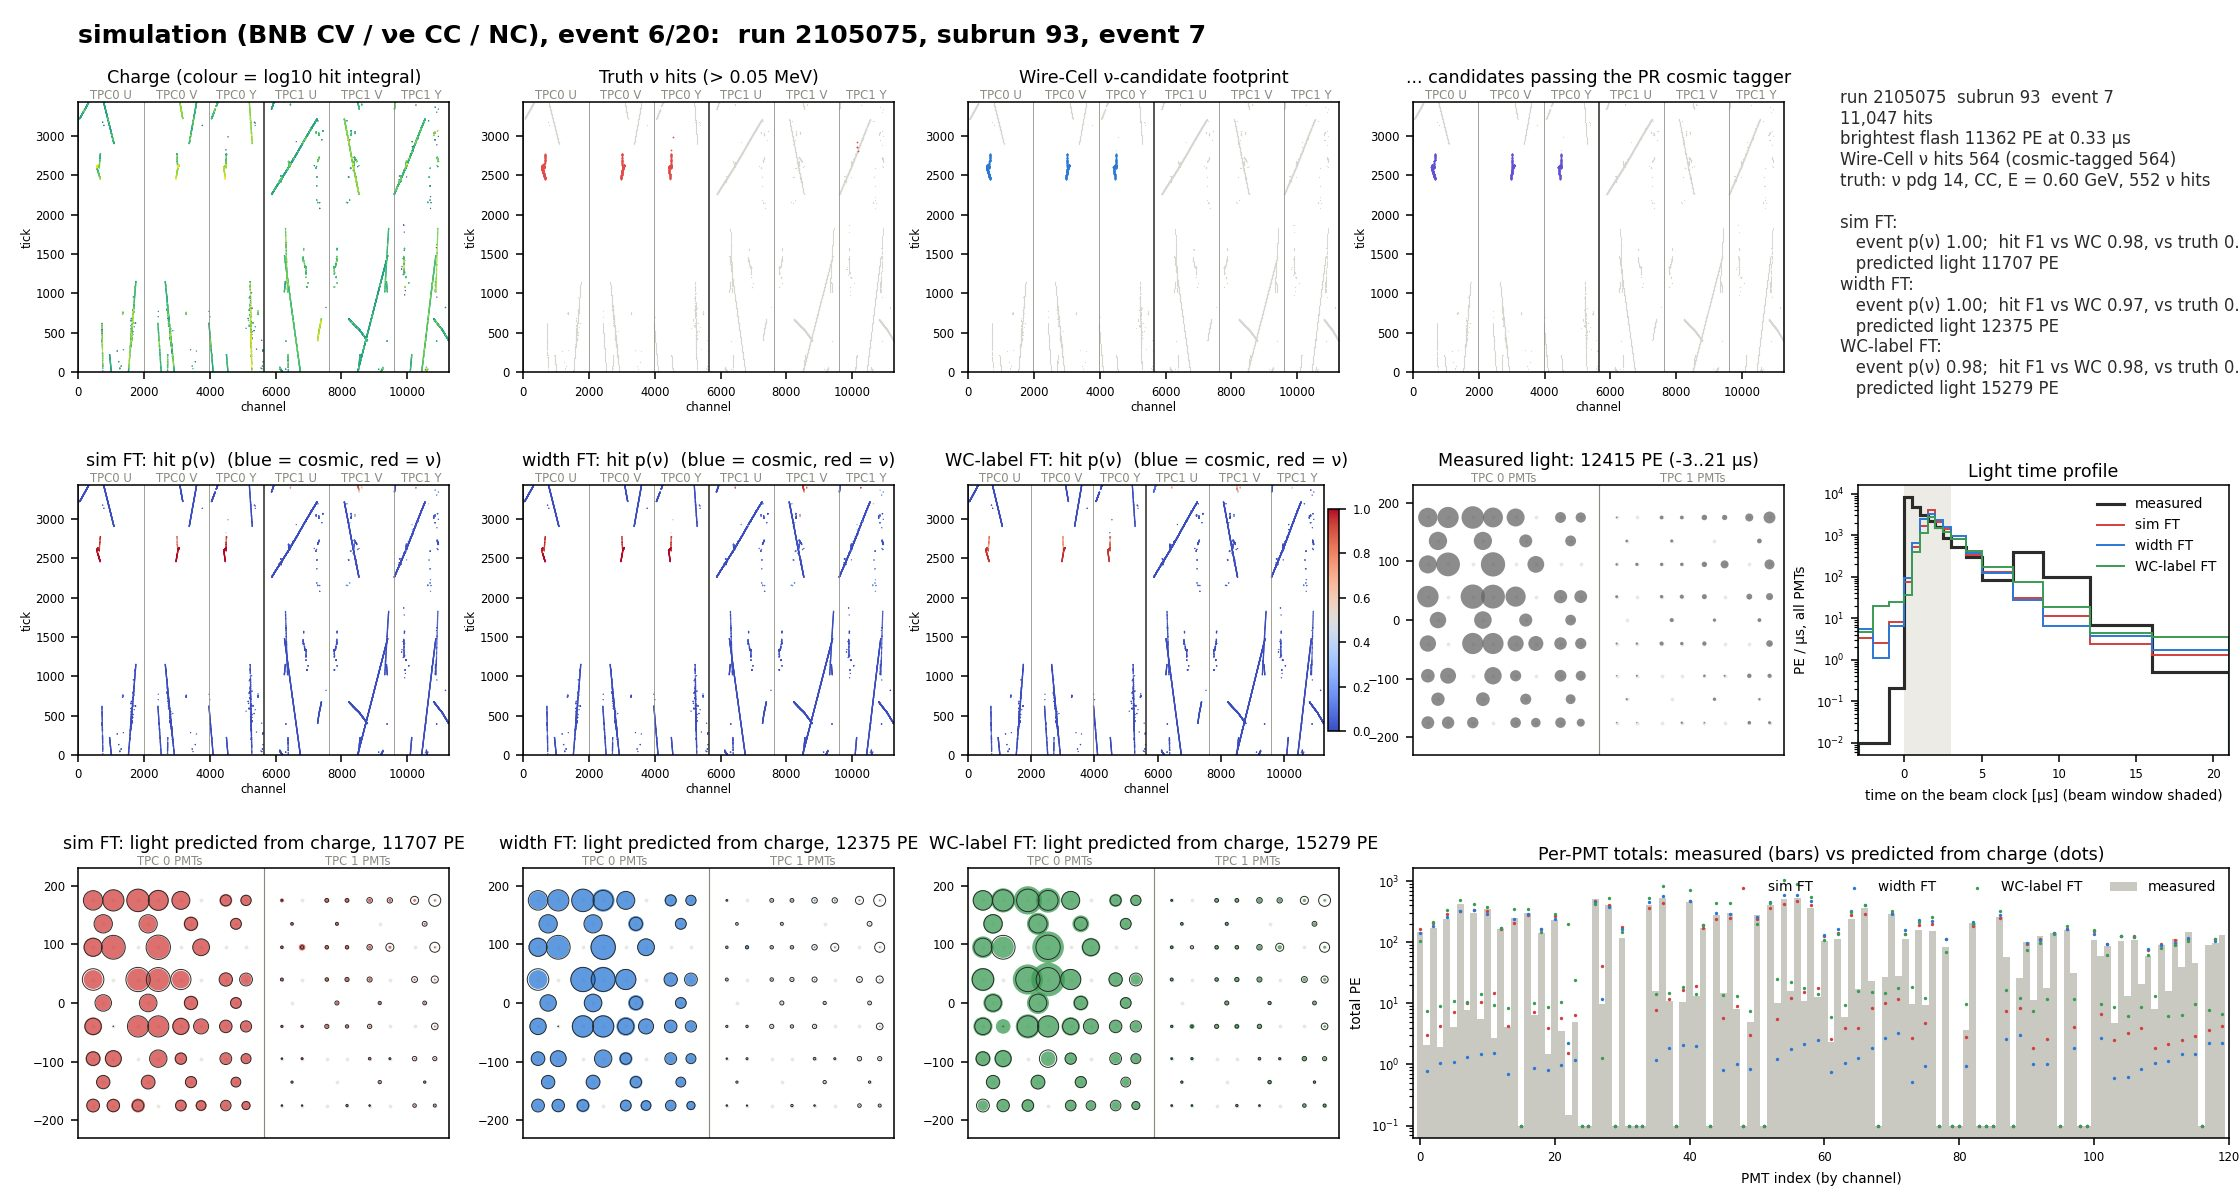
\includegraphics[width=\paperwidth,height=\paperheight,keepaspectratio]{displays/sim_05.jpg}}
\end{frame}
% Simulation 7/20: run 2100060, subrun 93, event 5; event p(nu): sim FT 1.00, width FT 0.16, WC-label FT 0.61
\begin{frame}[plain]
  \centering\vspace*{-2pt}
  \makebox[\linewidth][c]{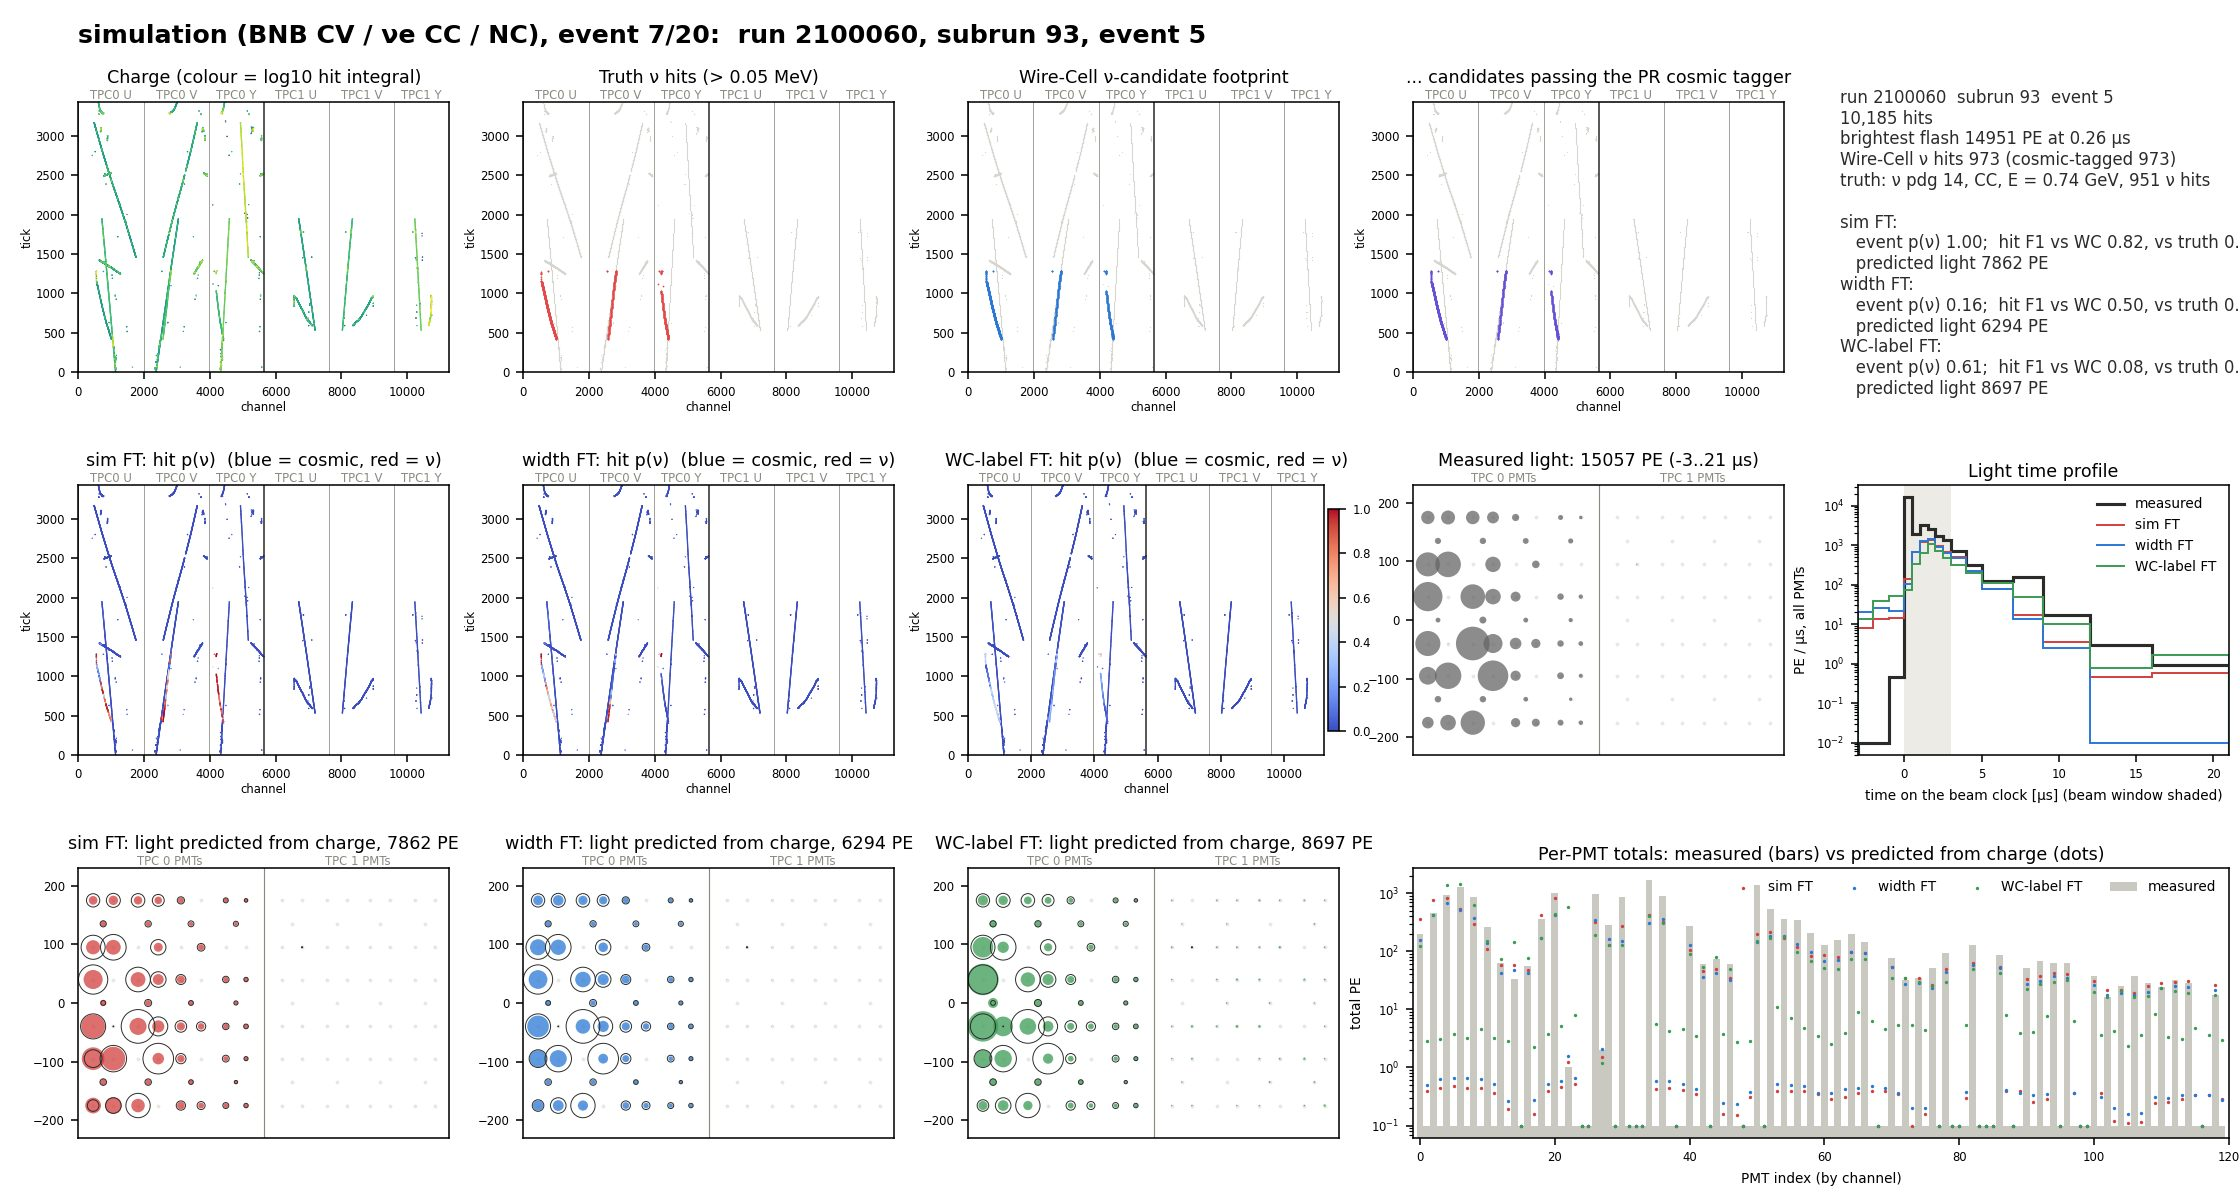
\includegraphics[width=\paperwidth,height=\paperheight,keepaspectratio]{displays/sim_06.jpg}}
\end{frame}
% Simulation 8/20: run 2100197, subrun 83, event 1; event p(nu): sim FT 1.00, width FT 1.00, WC-label FT 0.94
\begin{frame}[plain]
  \centering\vspace*{-2pt}
  \makebox[\linewidth][c]{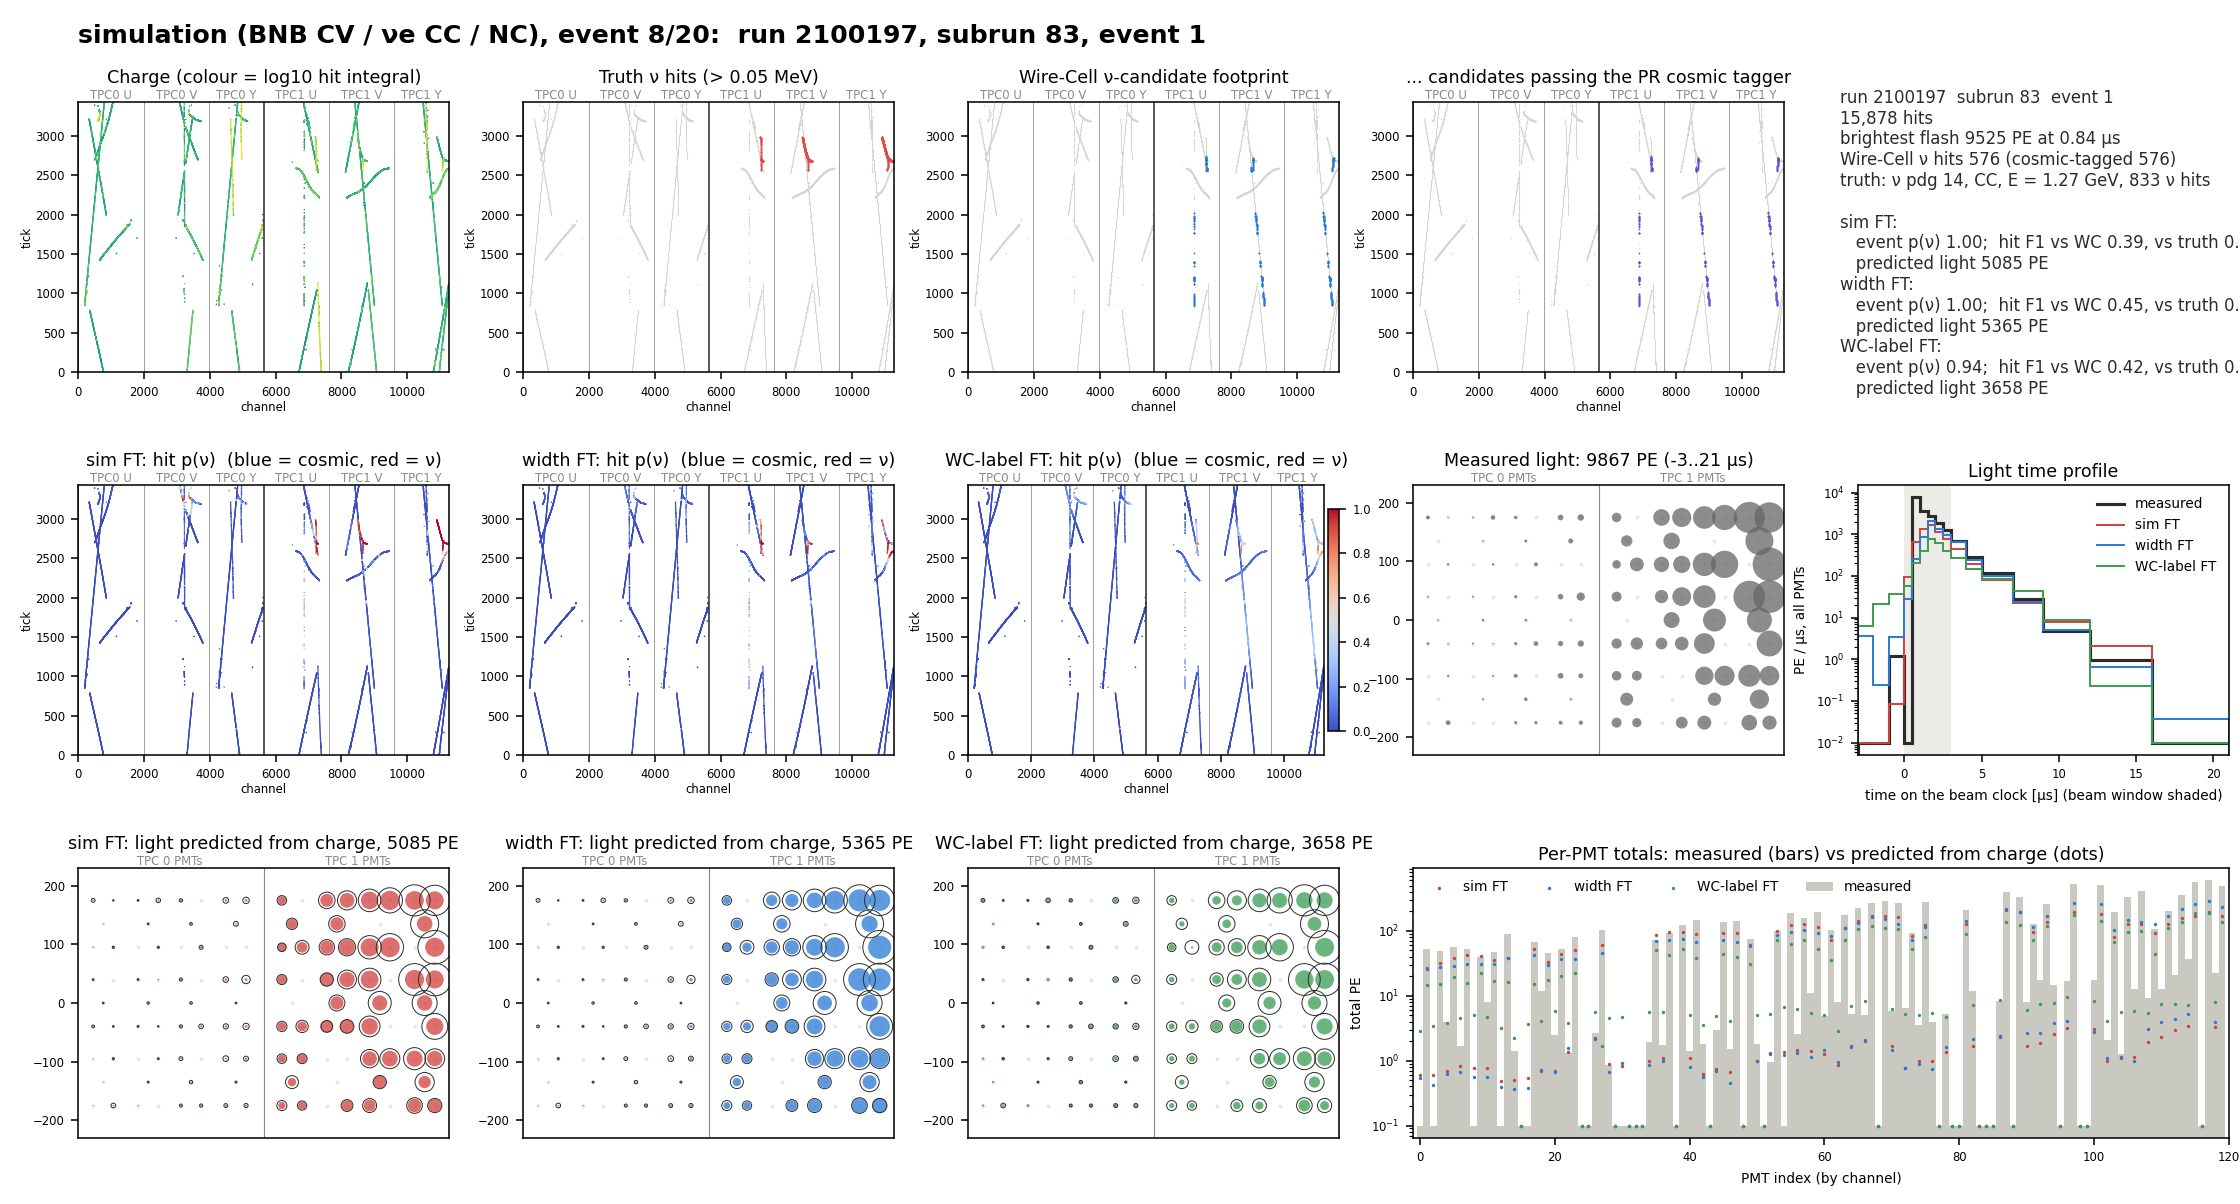
\includegraphics[width=\paperwidth,height=\paperheight,keepaspectratio]{displays/sim_07.jpg}}
\end{frame}
% Simulation 9/20: run 2100328, subrun 6, event 6; event p(nu): sim FT 1.00, width FT 1.00, WC-label FT 0.88
\begin{frame}[plain]
  \centering\vspace*{-2pt}
  \makebox[\linewidth][c]{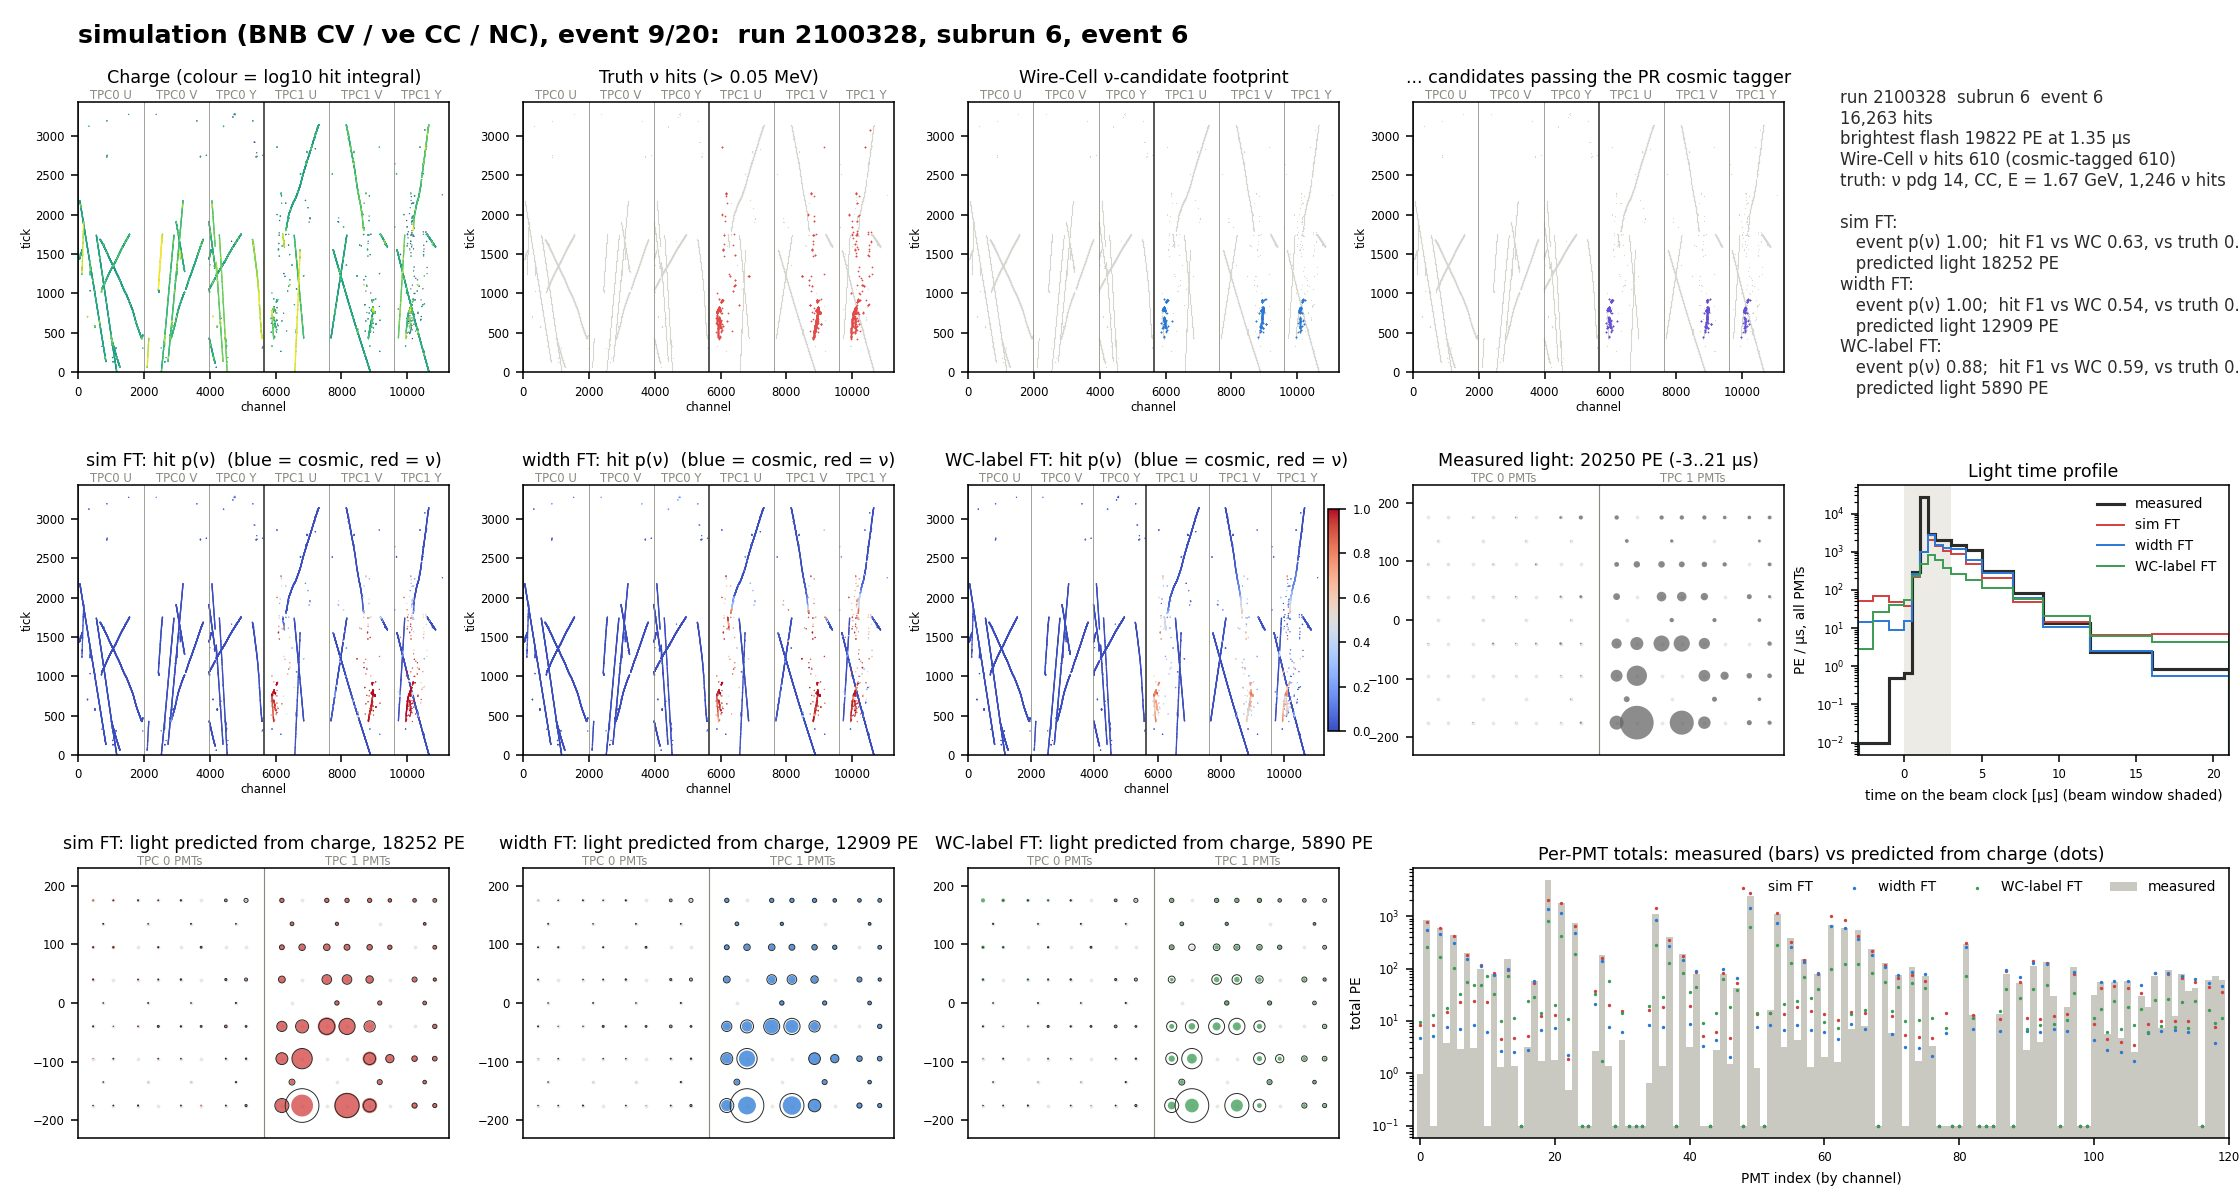
\includegraphics[width=\paperwidth,height=\paperheight,keepaspectratio]{displays/sim_08.jpg}}
\end{frame}
% Simulation 10/20: run 2100281, subrun 77, event 4; event p(nu): sim FT 0.00, width FT 0.00, WC-label FT 0.02
\begin{frame}[plain]
  \centering\vspace*{-2pt}
  \makebox[\linewidth][c]{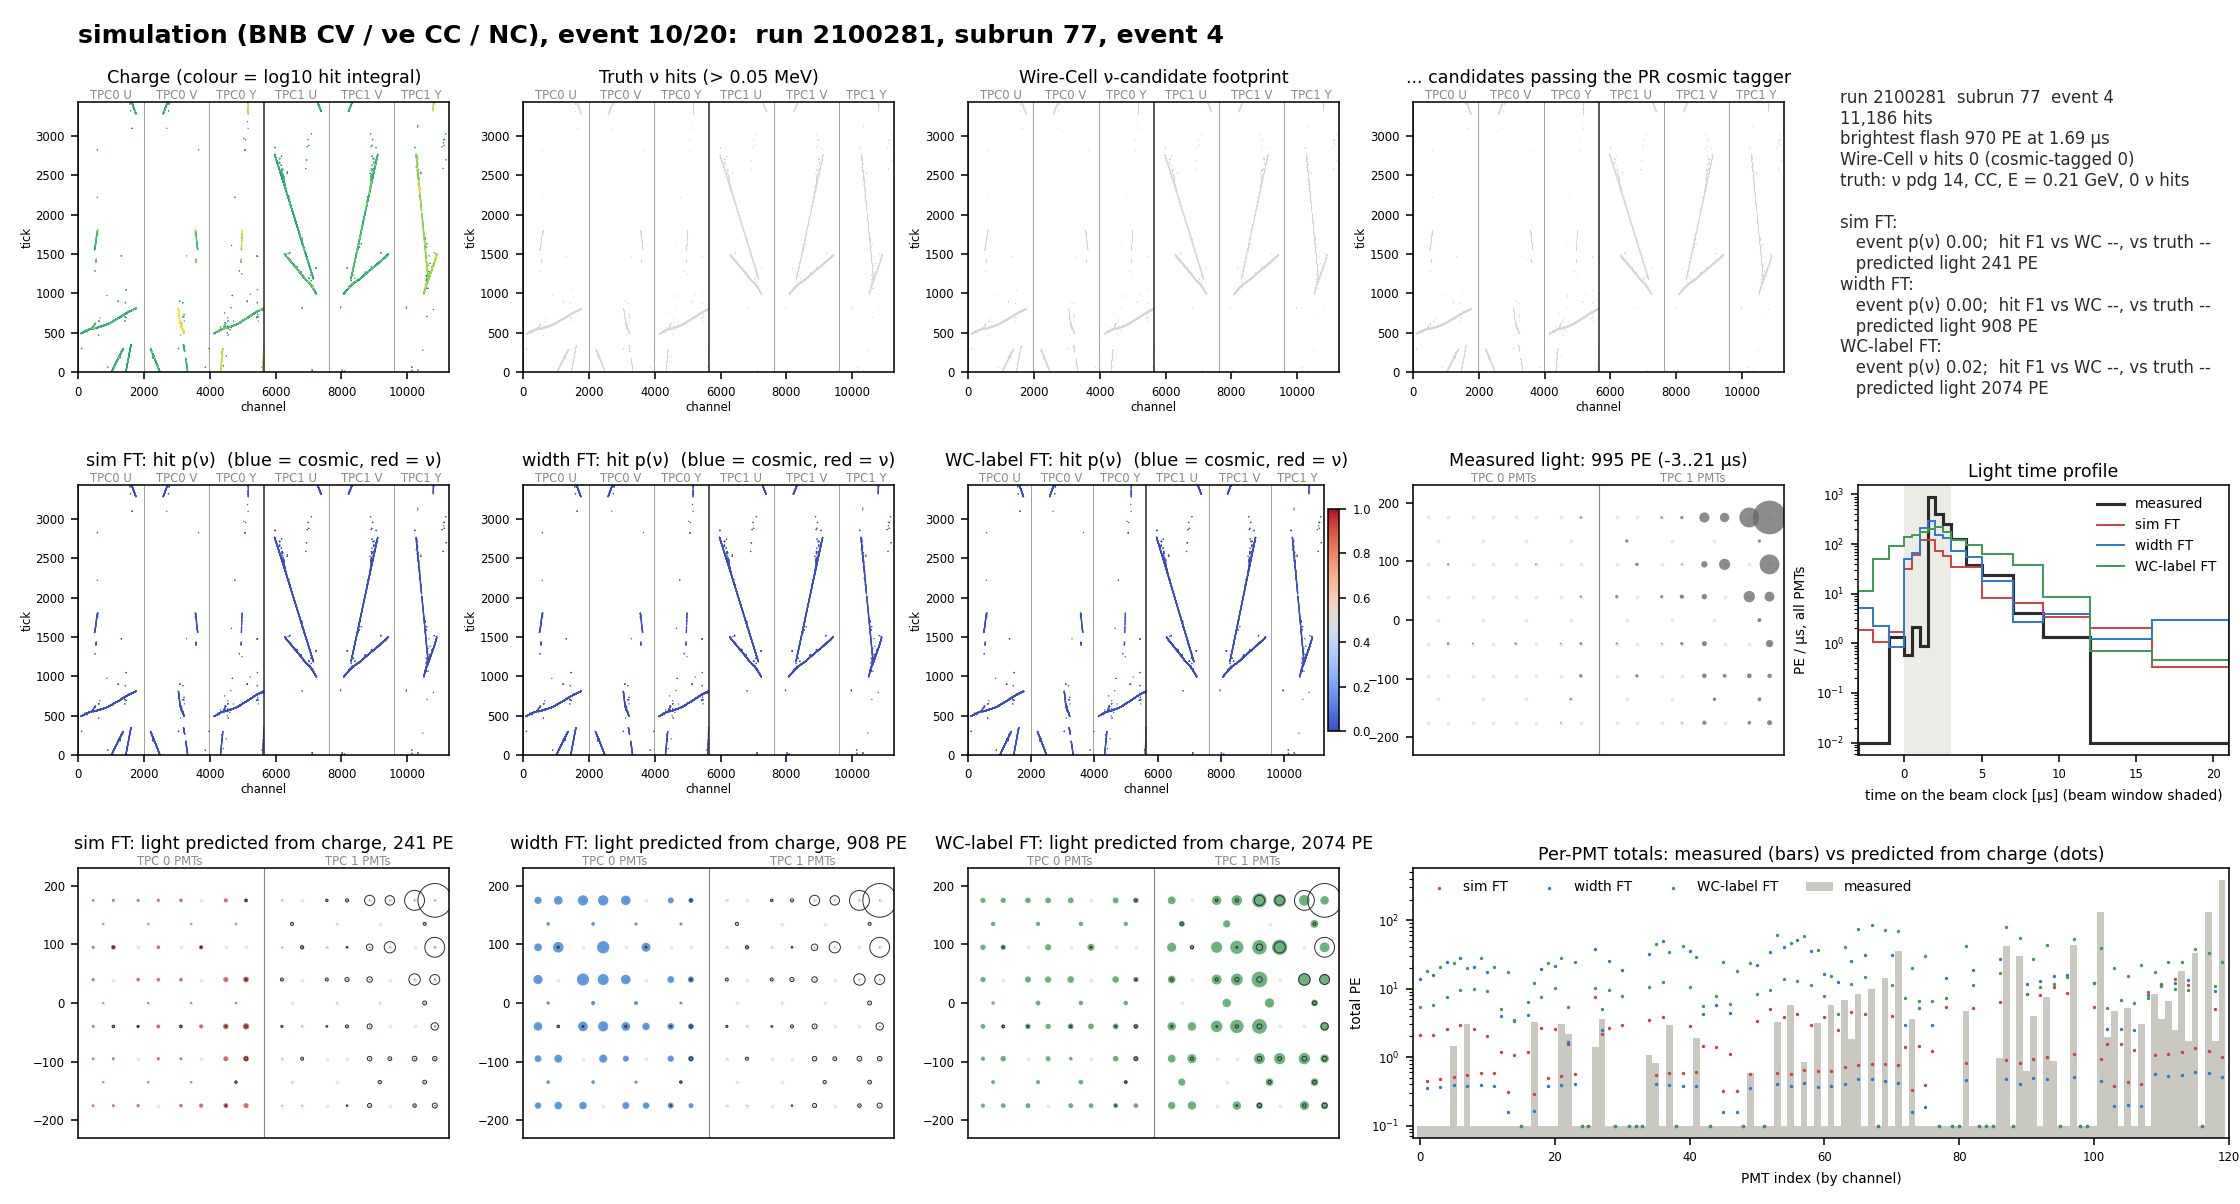
\includegraphics[width=\paperwidth,height=\paperheight,keepaspectratio]{displays/sim_09.jpg}}
\end{frame}
% Simulation 11/20: run 6708895, subrun 84, event 24; event p(nu): sim FT 1.00, width FT 1.00, WC-label FT 0.98
\begin{frame}[plain]
  \centering\vspace*{-2pt}
  \makebox[\linewidth][c]{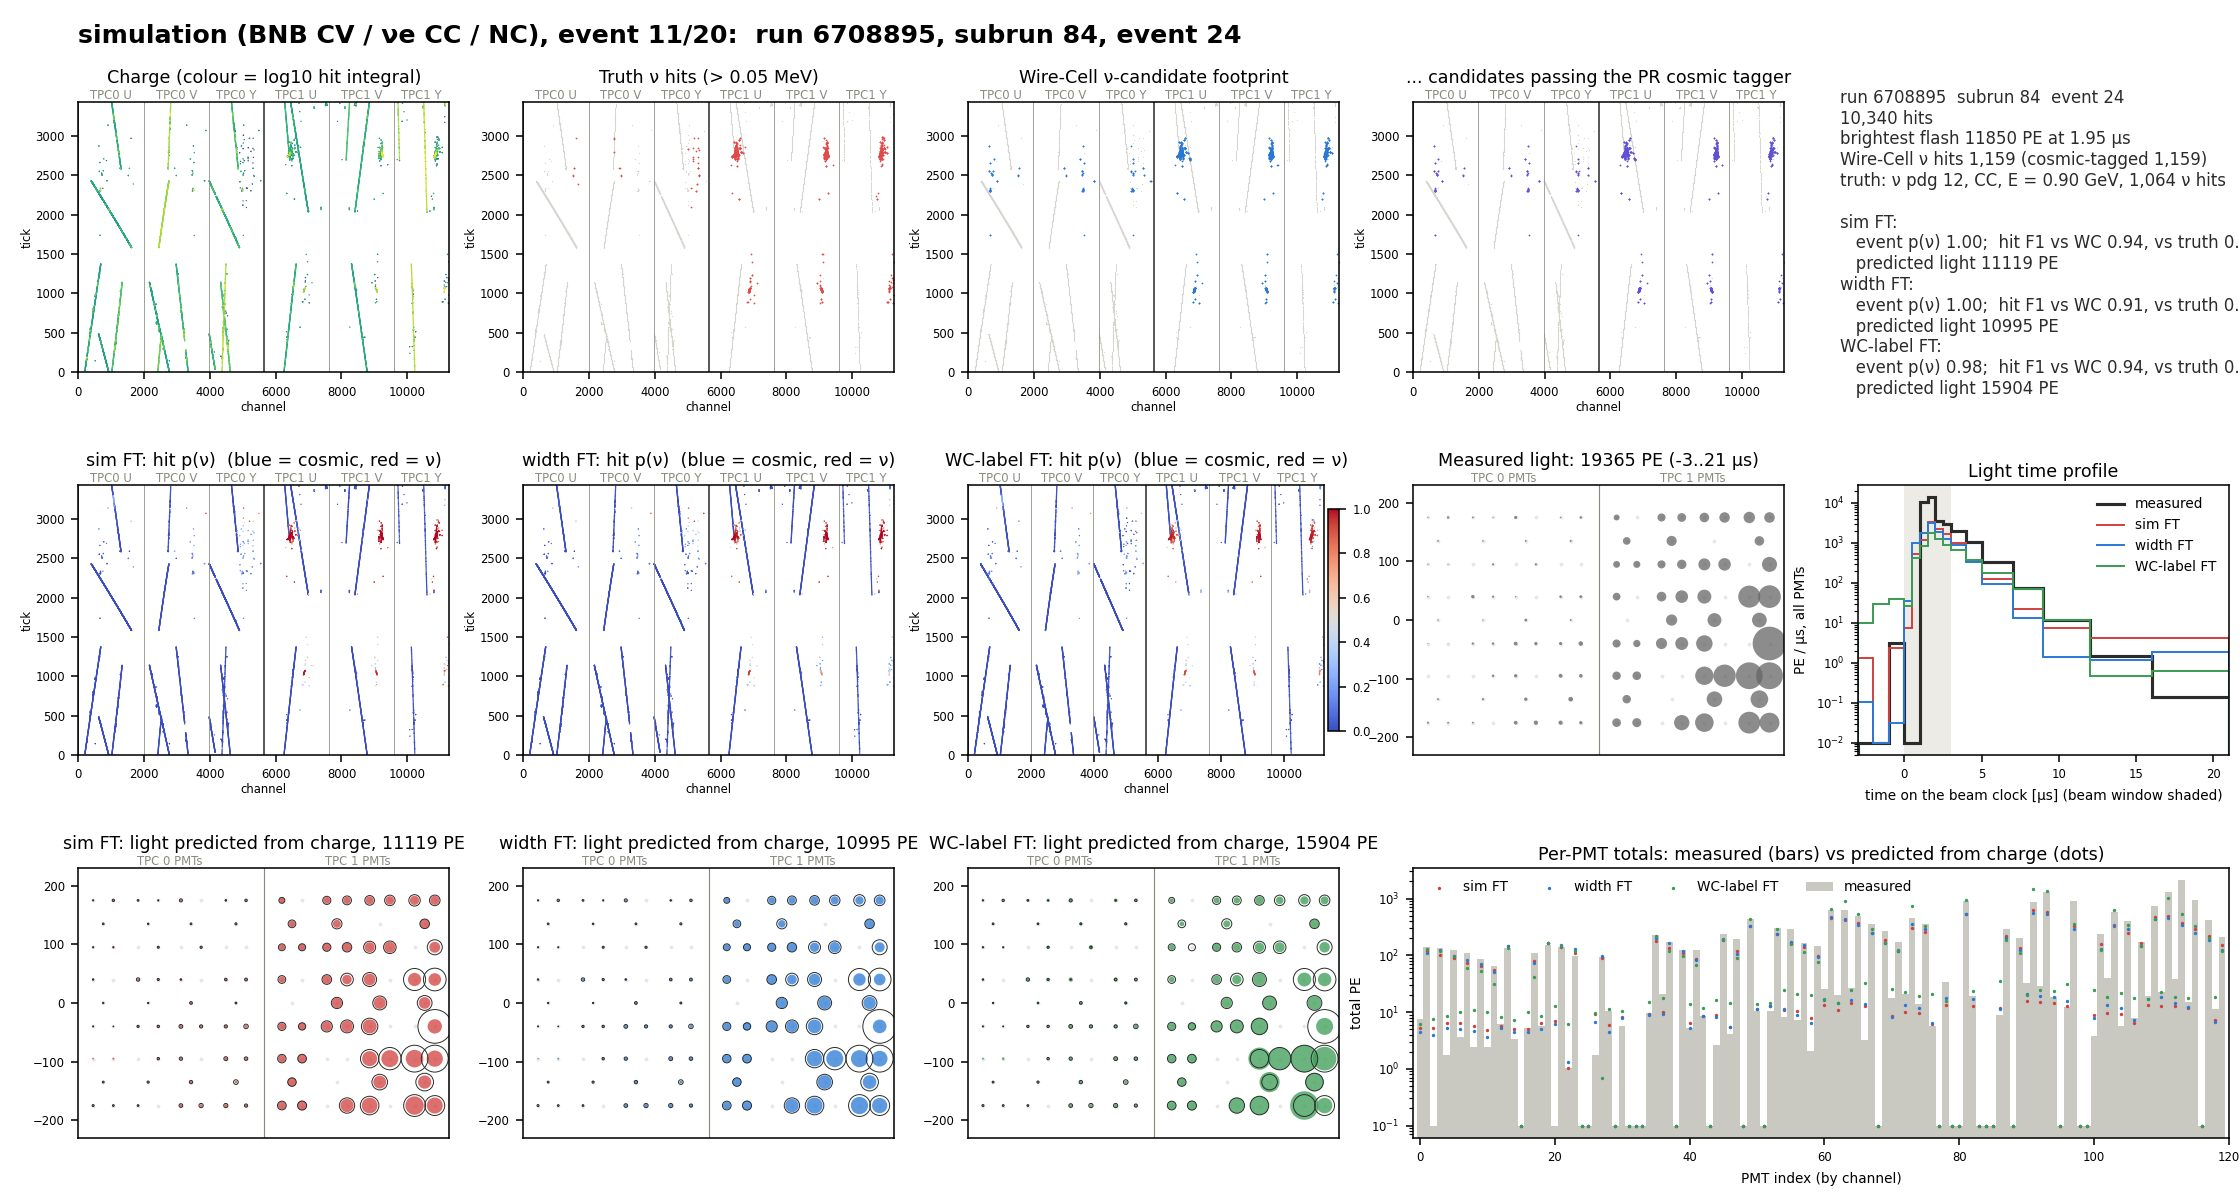
\includegraphics[width=\paperwidth,height=\paperheight,keepaspectratio]{displays/sim_10.jpg}}
\end{frame}
% Simulation 12/20: run 6709684, subrun 21, event 109; event p(nu): sim FT 1.00, width FT 1.00, WC-label FT 0.94
\begin{frame}[plain]
  \centering\vspace*{-2pt}
  \makebox[\linewidth][c]{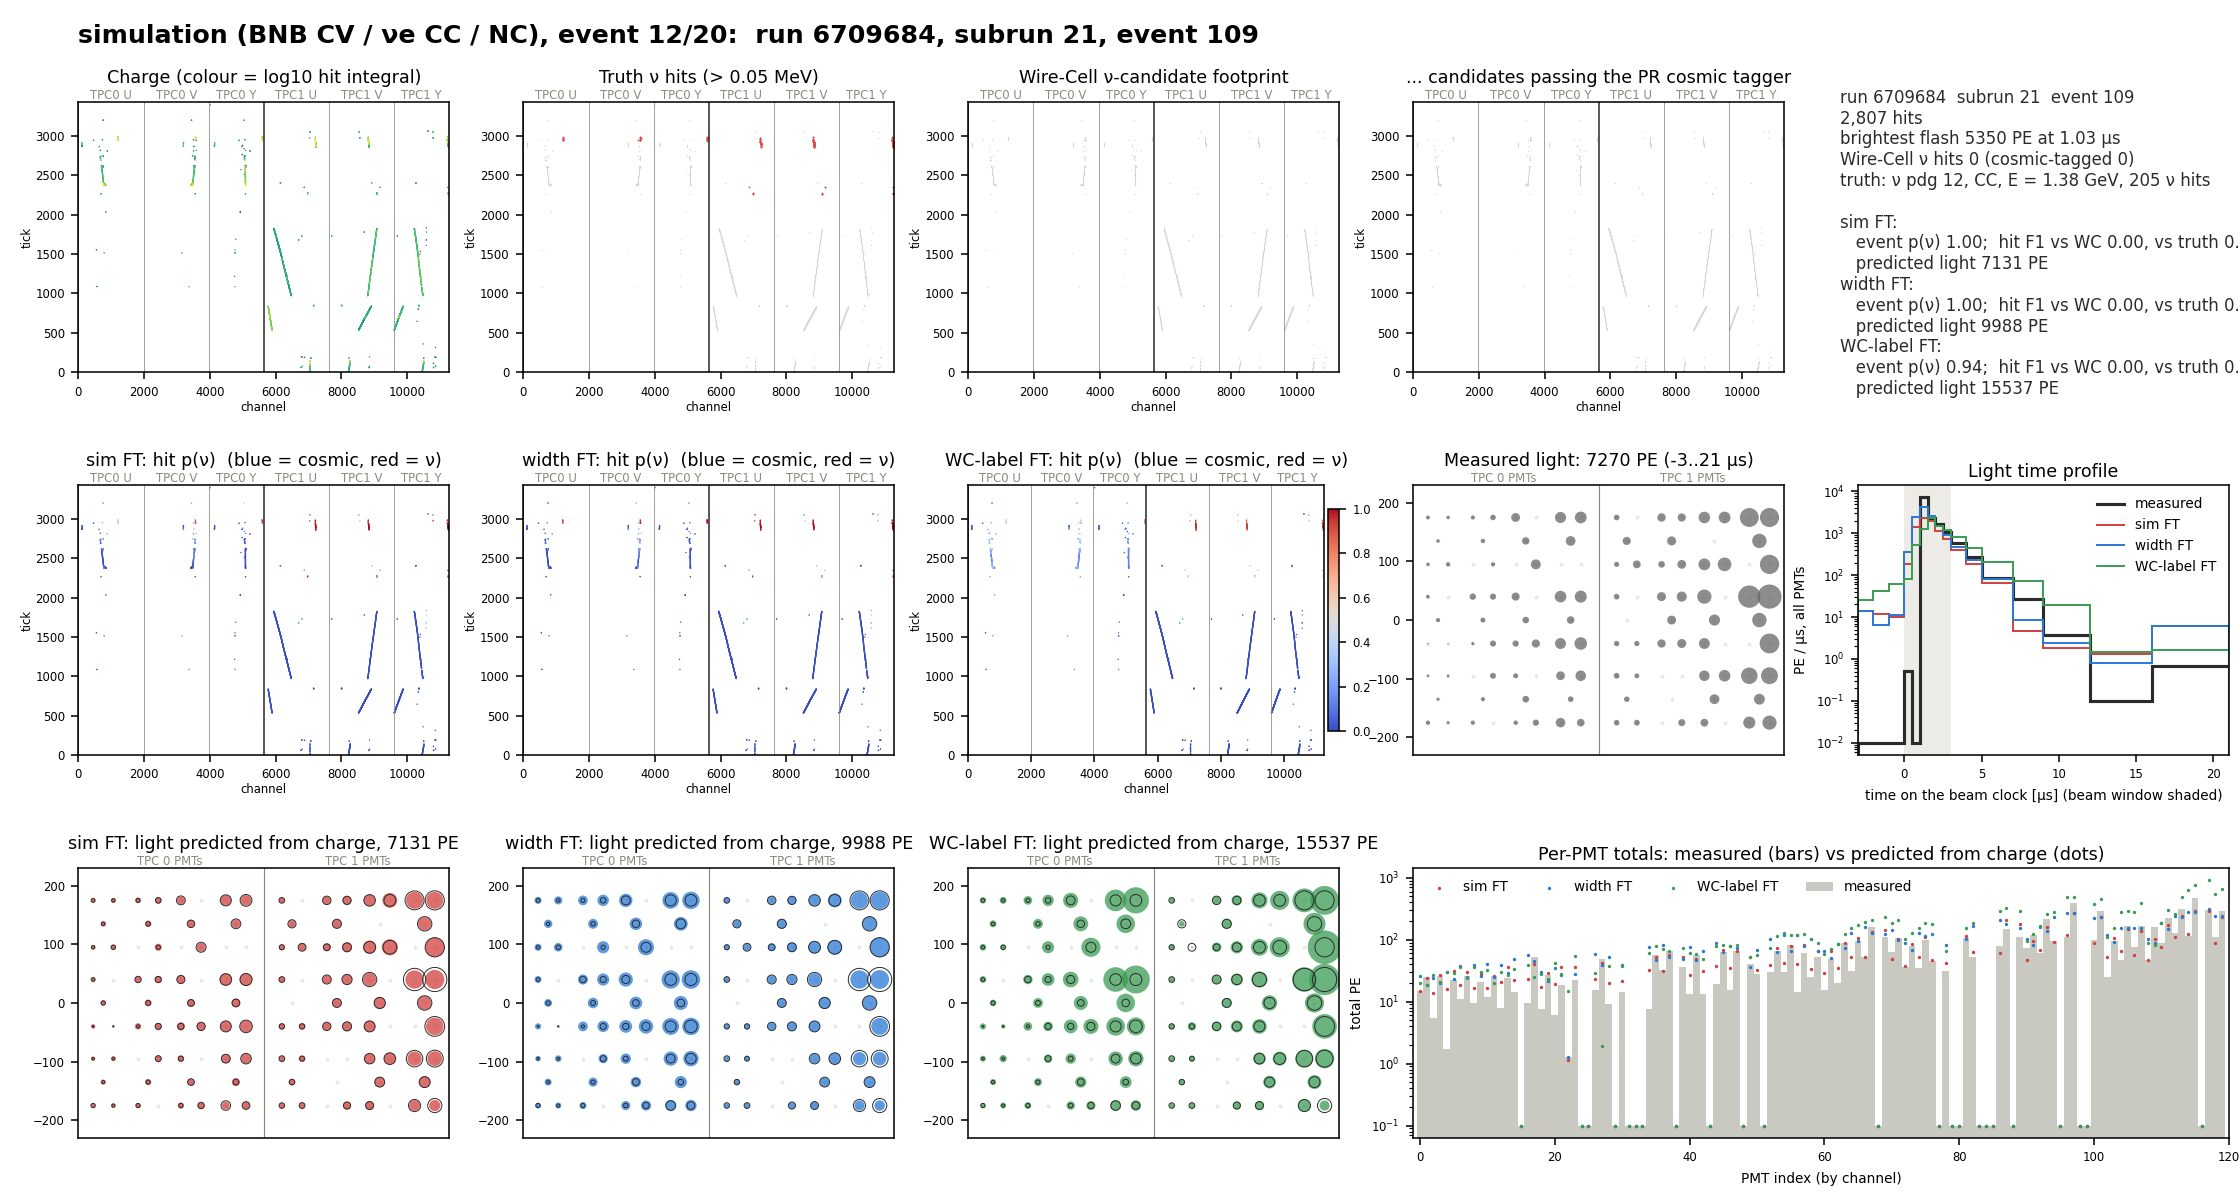
\includegraphics[width=\paperwidth,height=\paperheight,keepaspectratio]{displays/sim_11.jpg}}
\end{frame}
% Simulation 13/20: run 6725872, subrun 6, event 39; event p(nu): sim FT 1.00, width FT 1.00, WC-label FT 0.98
\begin{frame}[plain]
  \centering\vspace*{-2pt}
  \makebox[\linewidth][c]{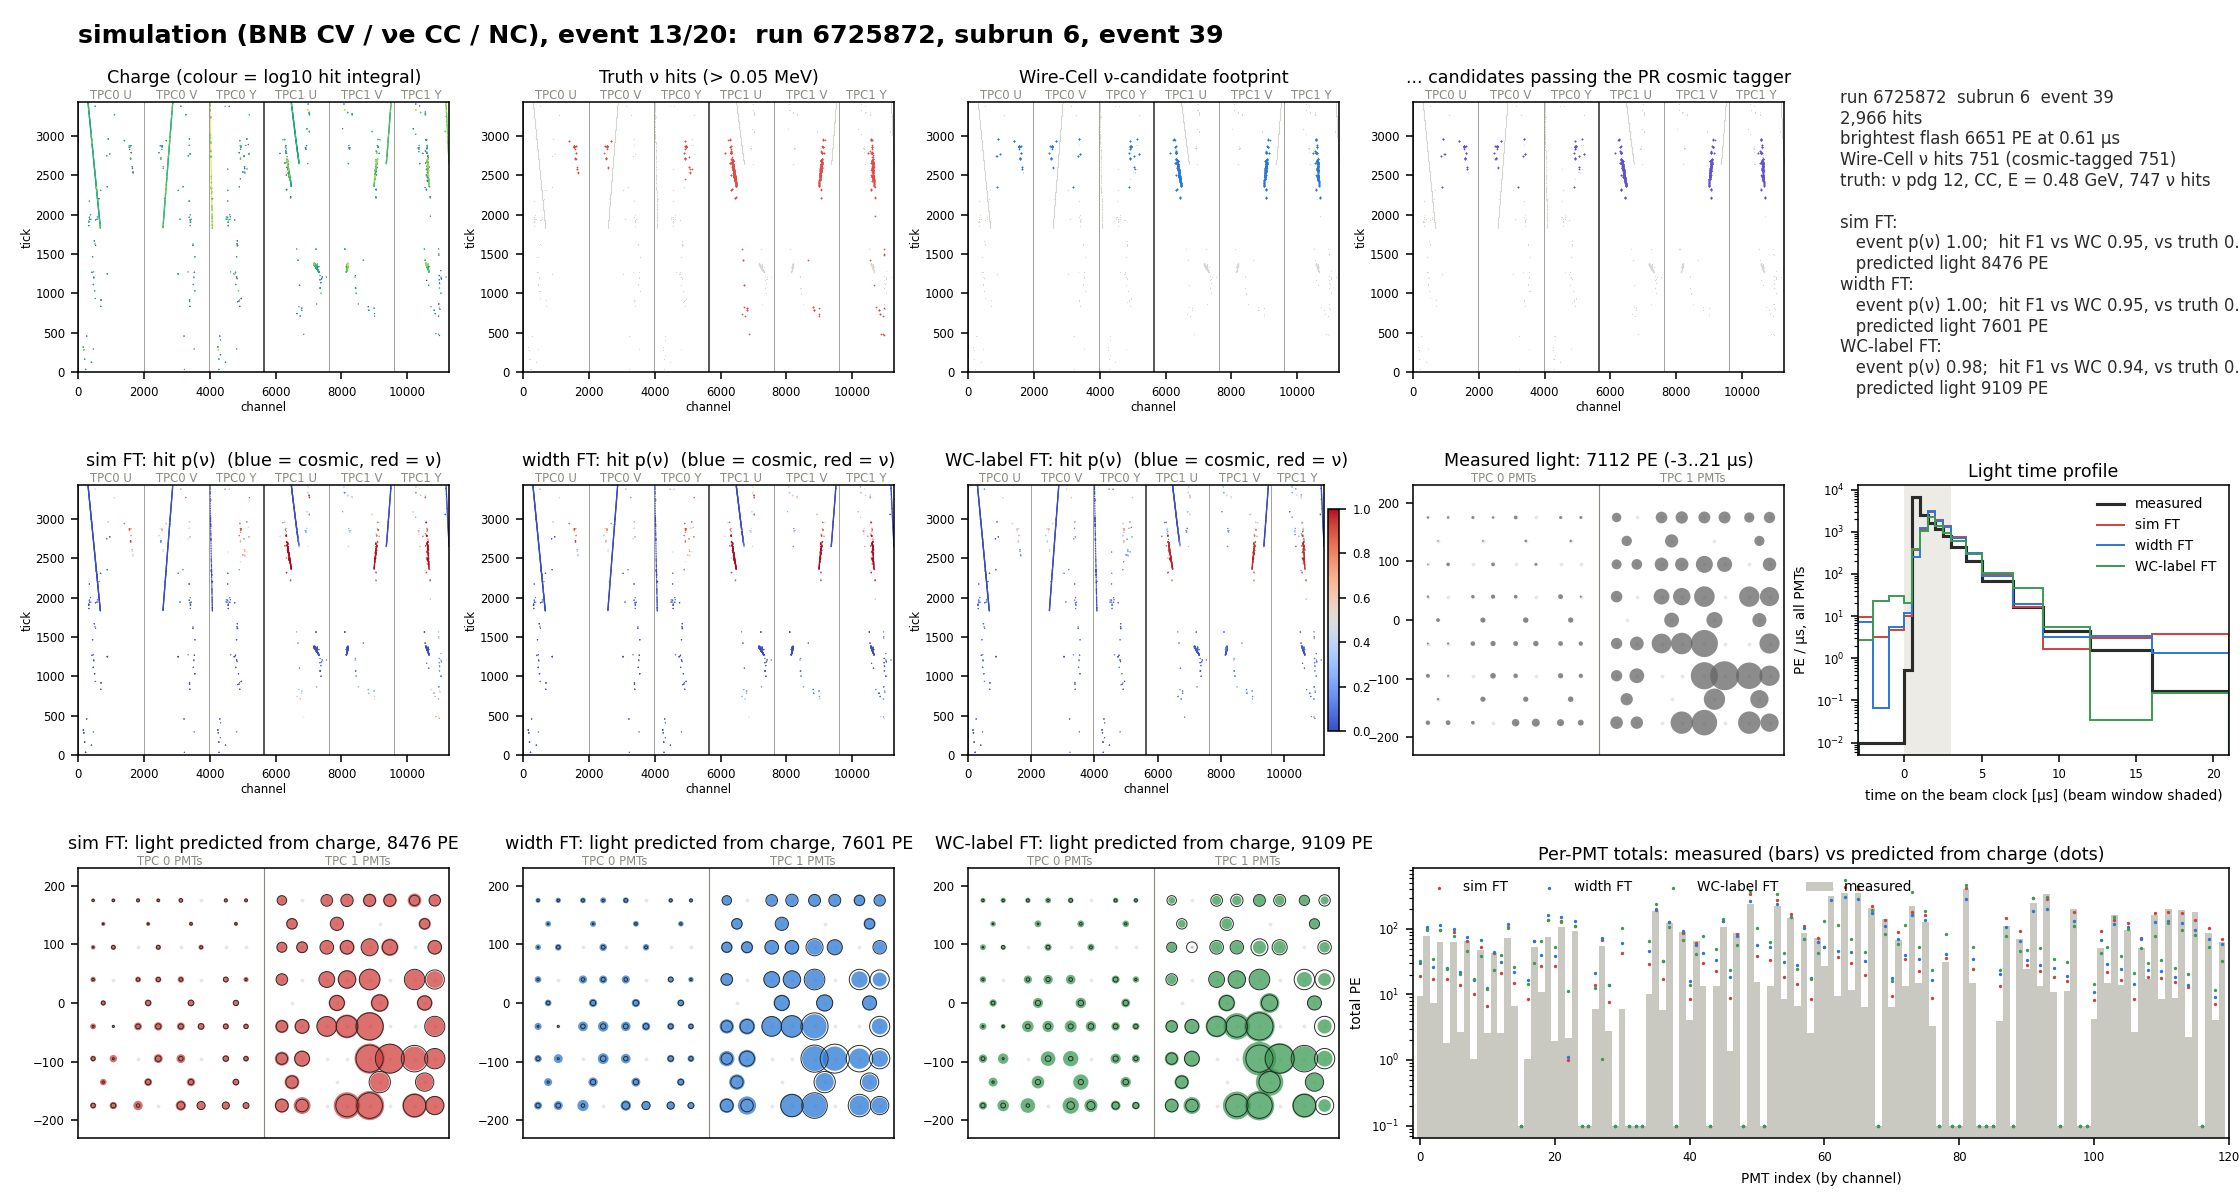
\includegraphics[width=\paperwidth,height=\paperheight,keepaspectratio]{displays/sim_12.jpg}}
\end{frame}
% Simulation 14/20: run 6731633, subrun 49, event 68; event p(nu): sim FT 1.00, width FT 1.00, WC-label FT 0.99
\begin{frame}[plain]
  \centering\vspace*{-2pt}
  \makebox[\linewidth][c]{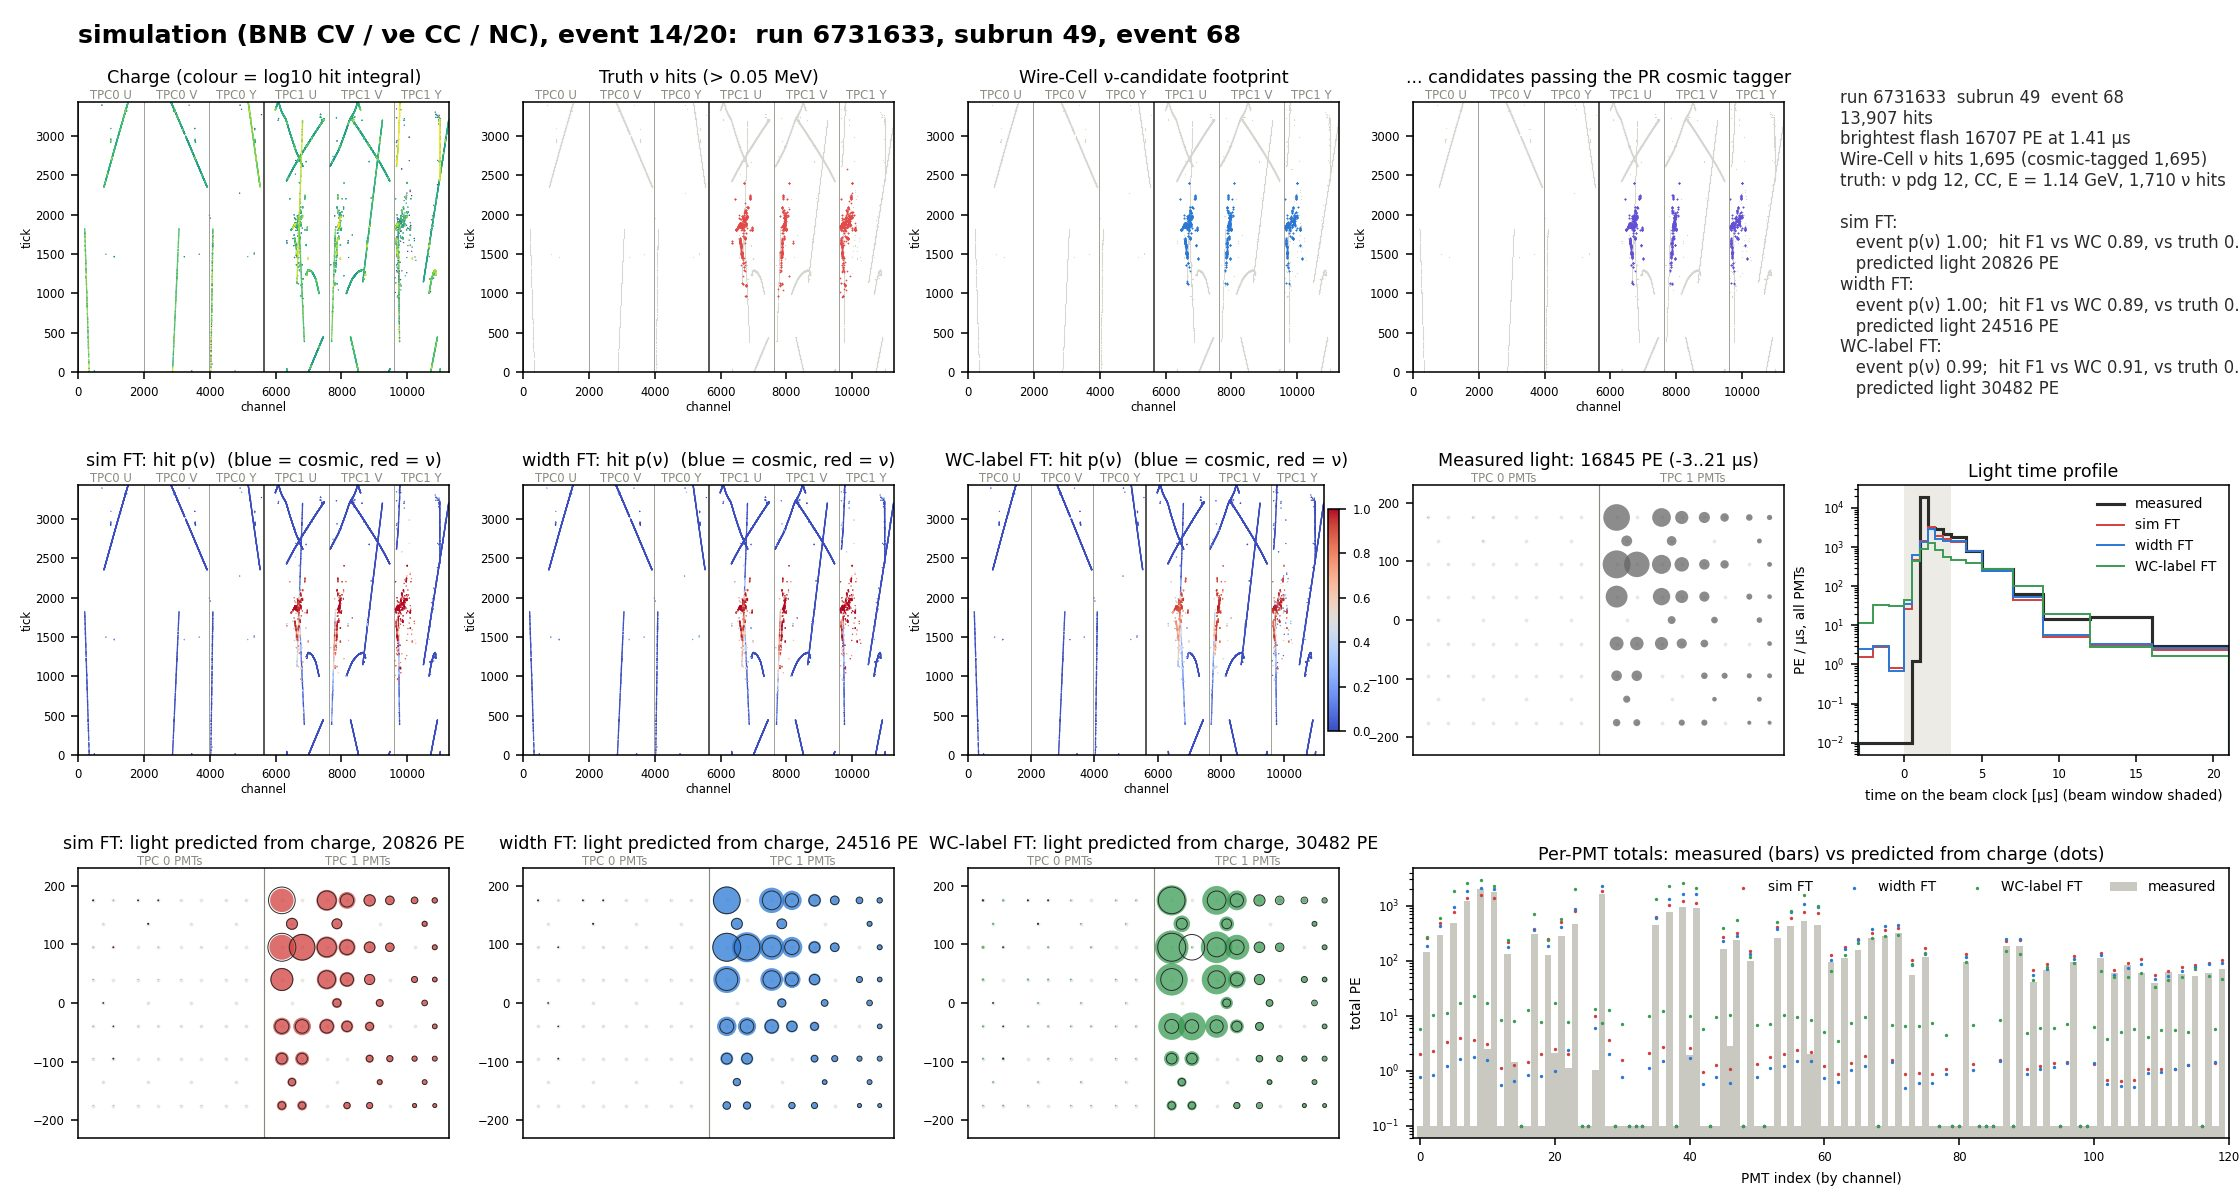
\includegraphics[width=\paperwidth,height=\paperheight,keepaspectratio]{displays/sim_13.jpg}}
\end{frame}
% Simulation 15/20: run 6701731, subrun 3, event 92; event p(nu): sim FT 1.00, width FT 1.00, WC-label FT 0.99
\begin{frame}[plain]
  \centering\vspace*{-2pt}
  \makebox[\linewidth][c]{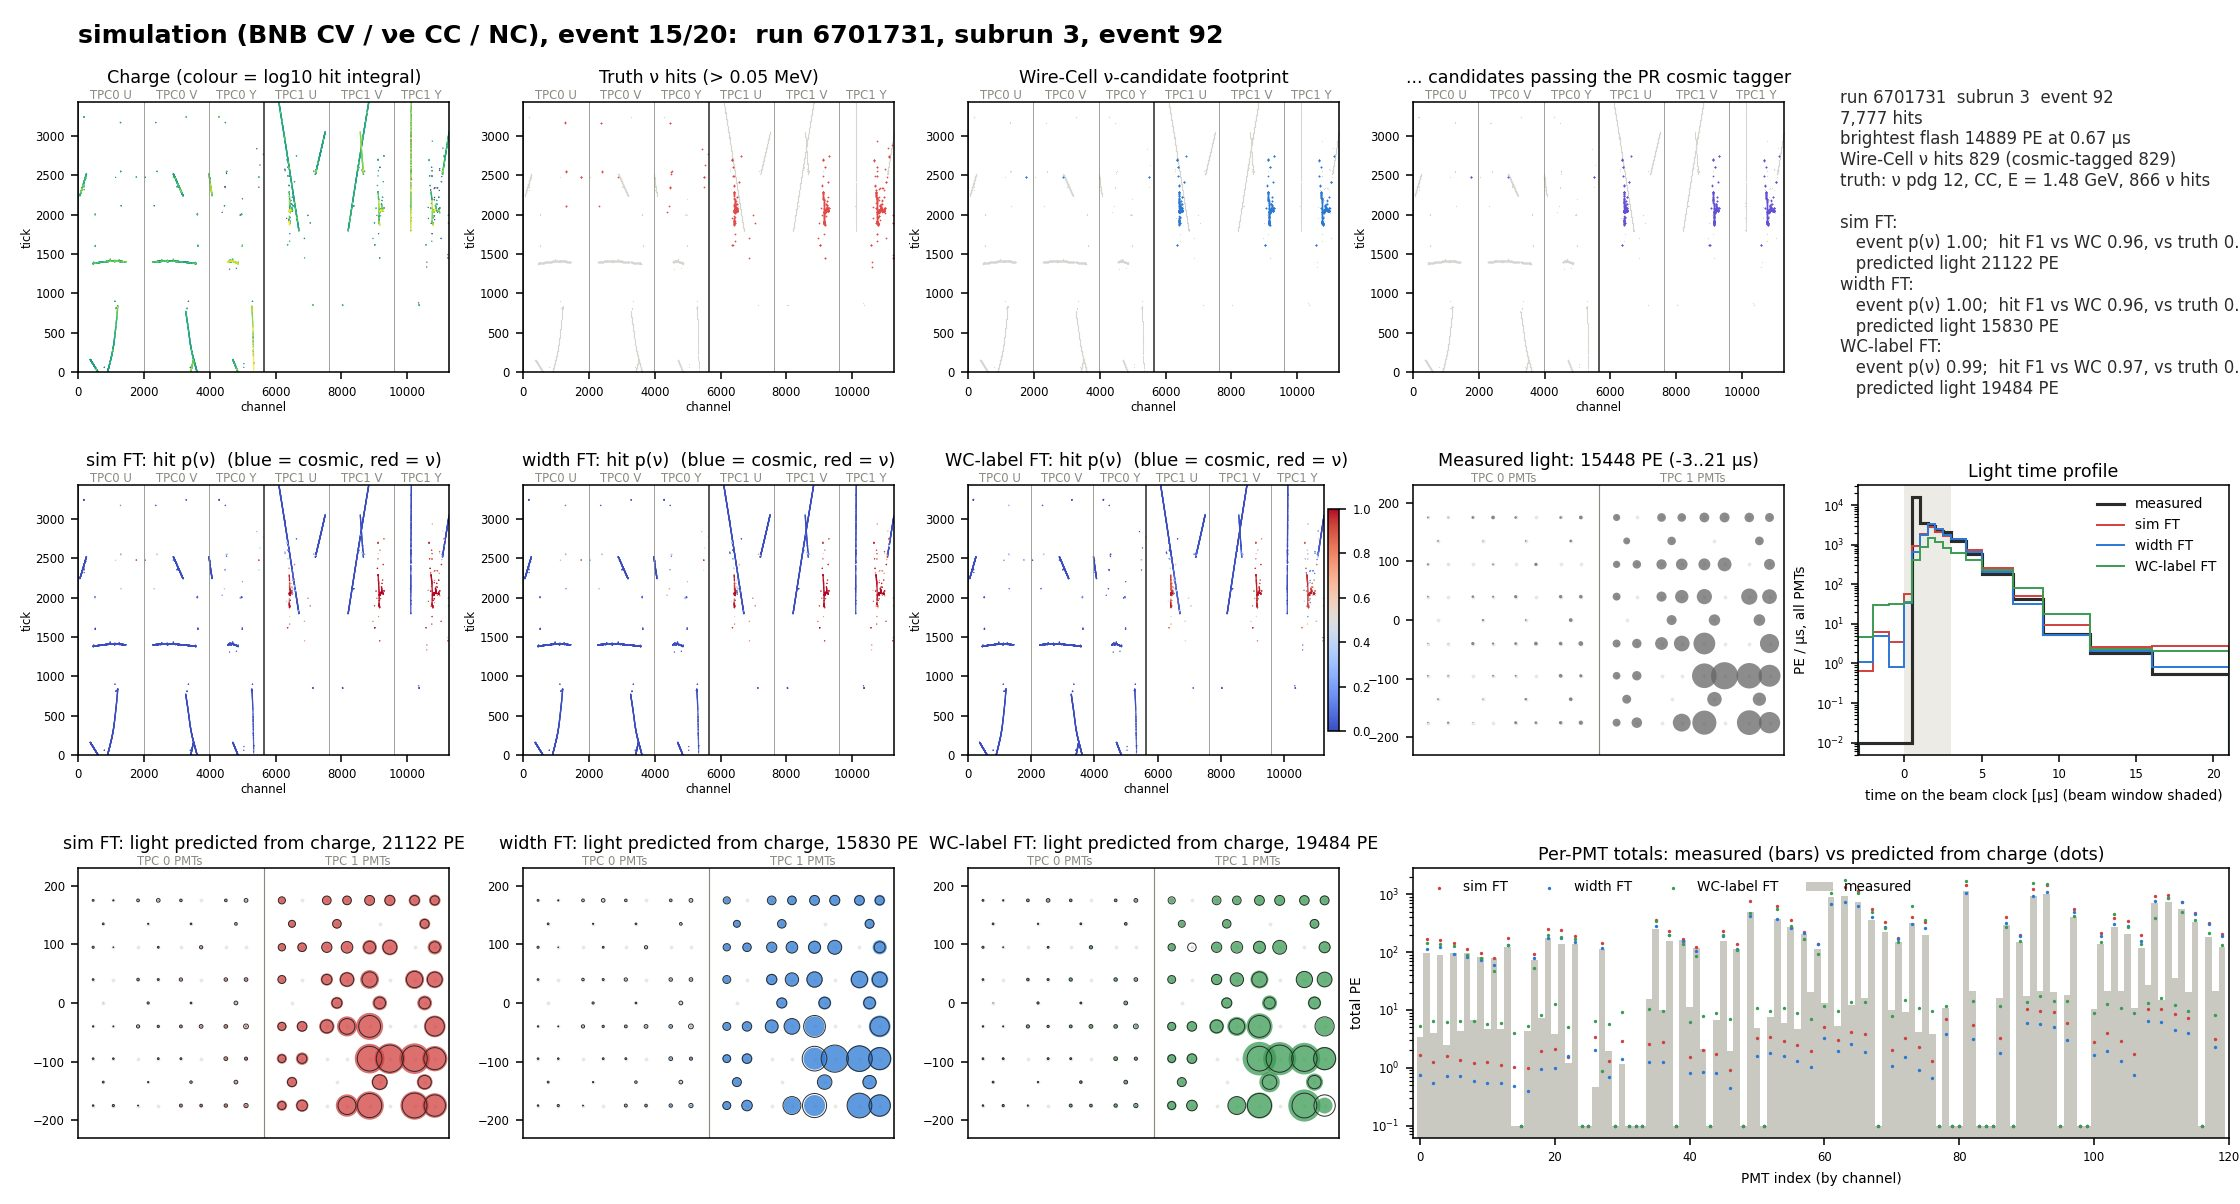
\includegraphics[width=\paperwidth,height=\paperheight,keepaspectratio]{displays/sim_14.jpg}}
\end{frame}
% Simulation 16/20: run 6712578, subrun 67, event 77; event p(nu): sim FT 1.00, width FT 1.00, WC-label FT 1.00
\begin{frame}[plain]
  \centering\vspace*{-2pt}
  \makebox[\linewidth][c]{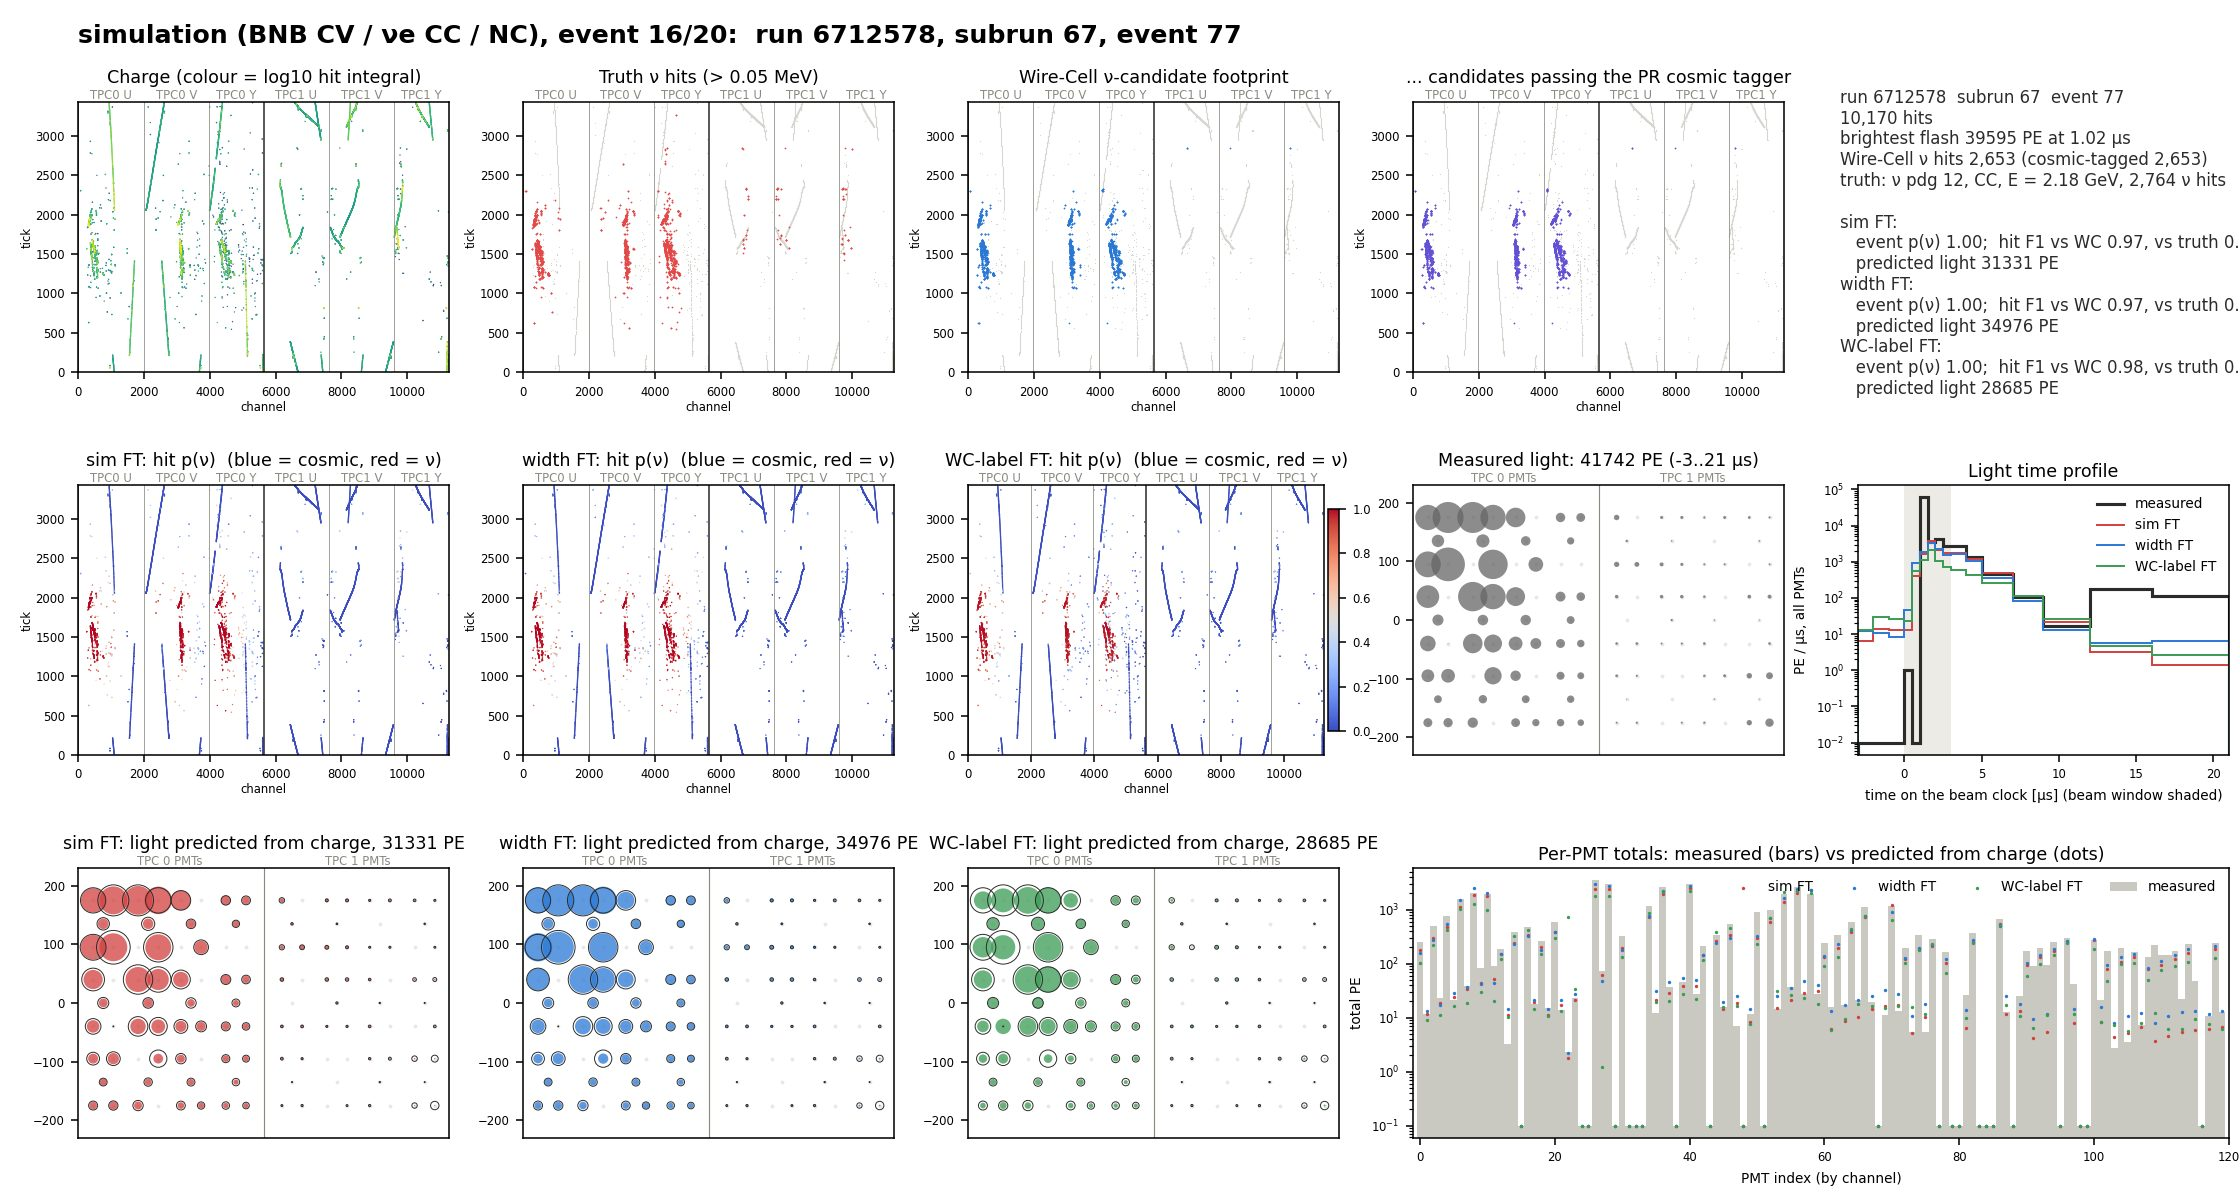
\includegraphics[width=\paperwidth,height=\paperheight,keepaspectratio]{displays/sim_15.jpg}}
\end{frame}
% Simulation 17/20: run 6714530, subrun 46, event 93; event p(nu): sim FT 1.00, width FT 1.00, WC-label FT 0.99
\begin{frame}[plain]
  \centering\vspace*{-2pt}
  \makebox[\linewidth][c]{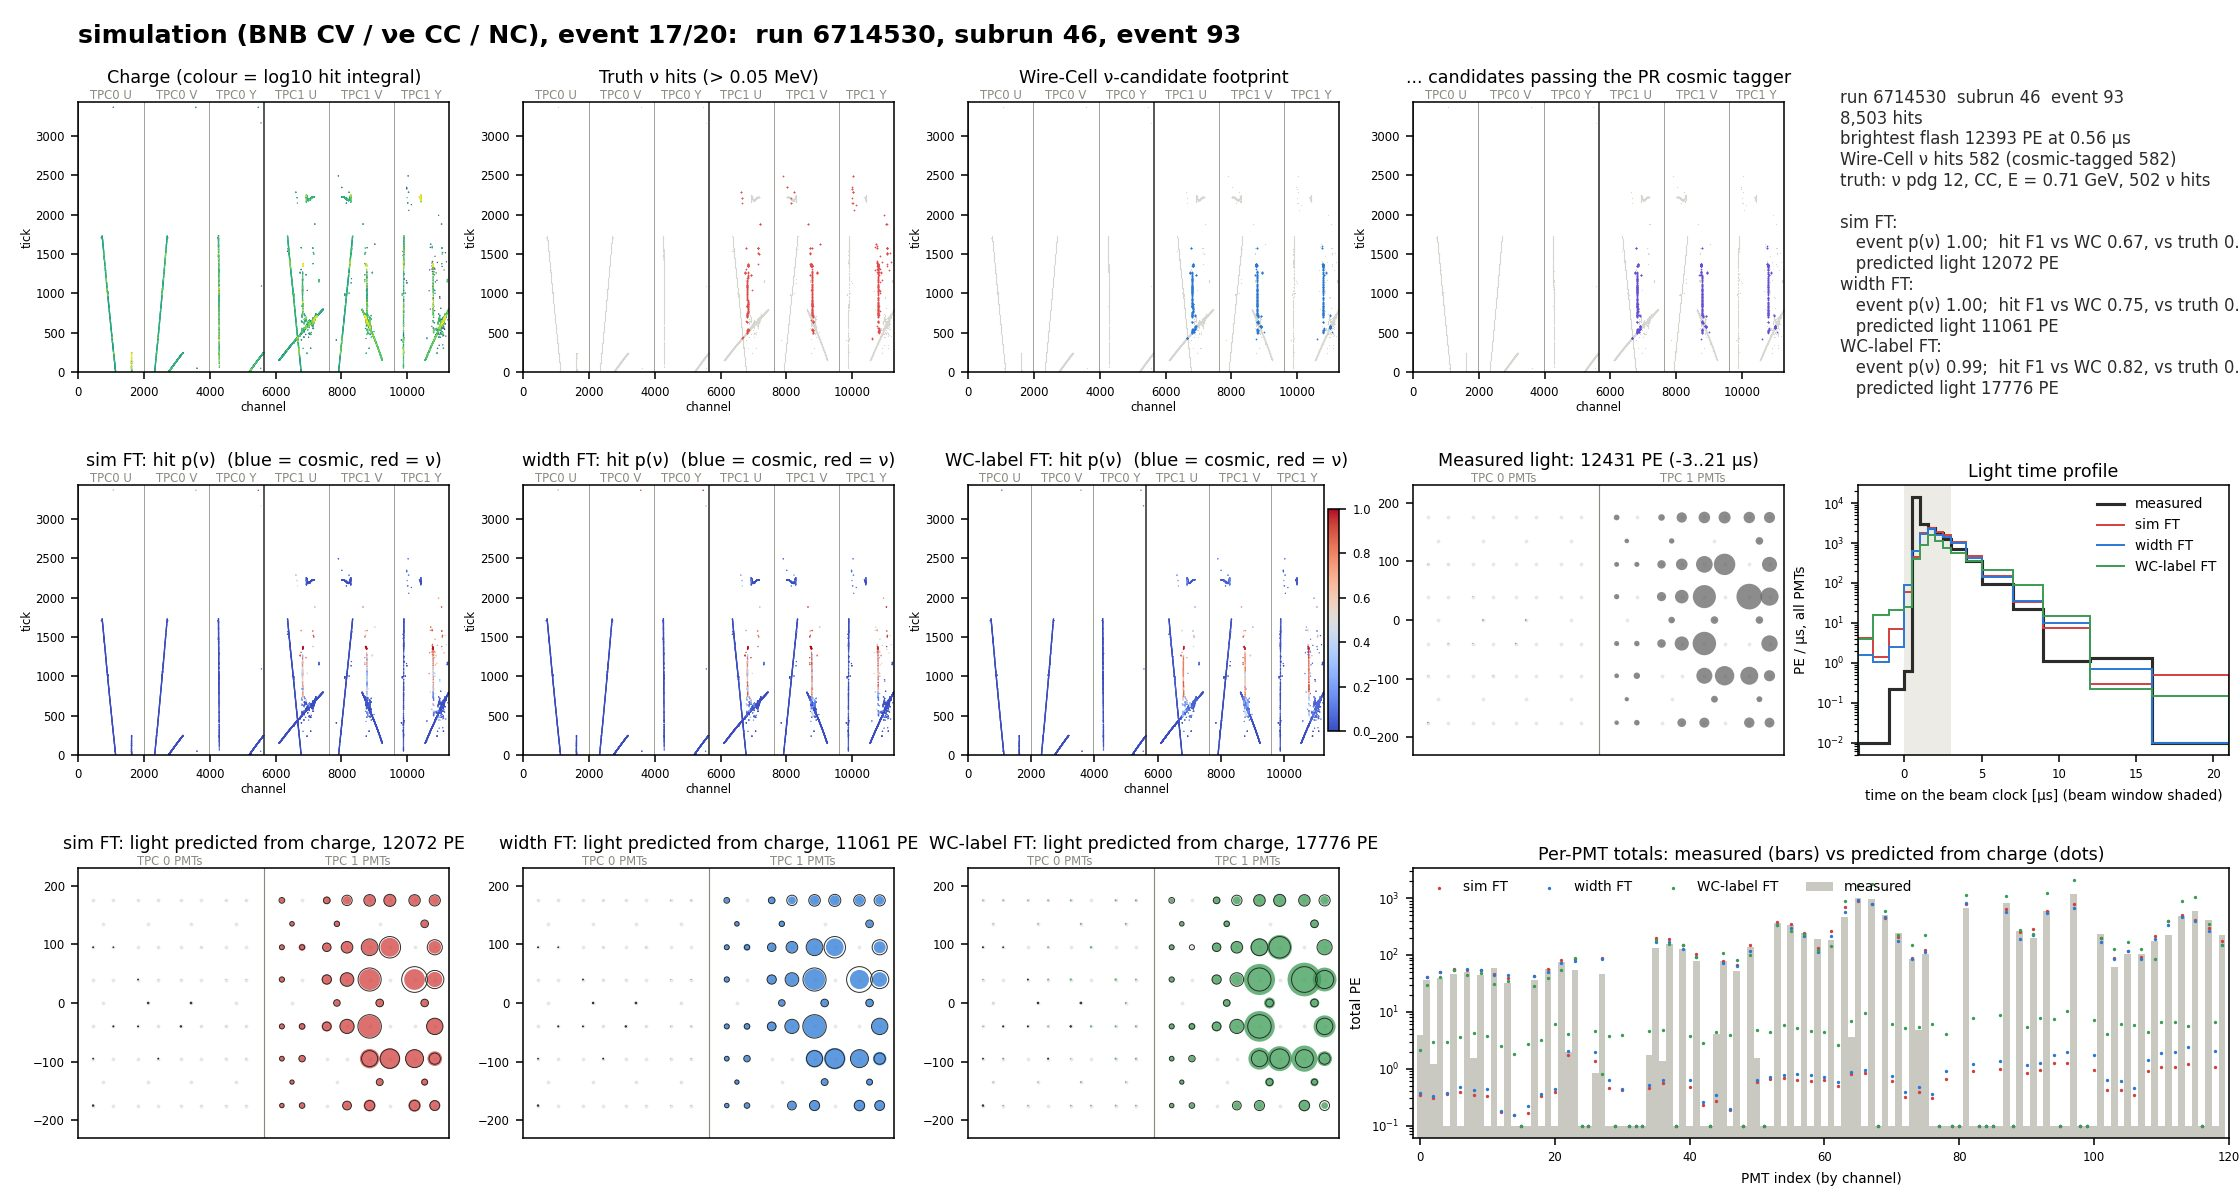
\includegraphics[width=\paperwidth,height=\paperheight,keepaspectratio]{displays/sim_16.jpg}}
\end{frame}
% Simulation 18/20: run 6712567, subrun 38, event 15; event p(nu): sim FT 1.00, width FT 1.00, WC-label FT 0.99
\begin{frame}[plain]
  \centering\vspace*{-2pt}
  \makebox[\linewidth][c]{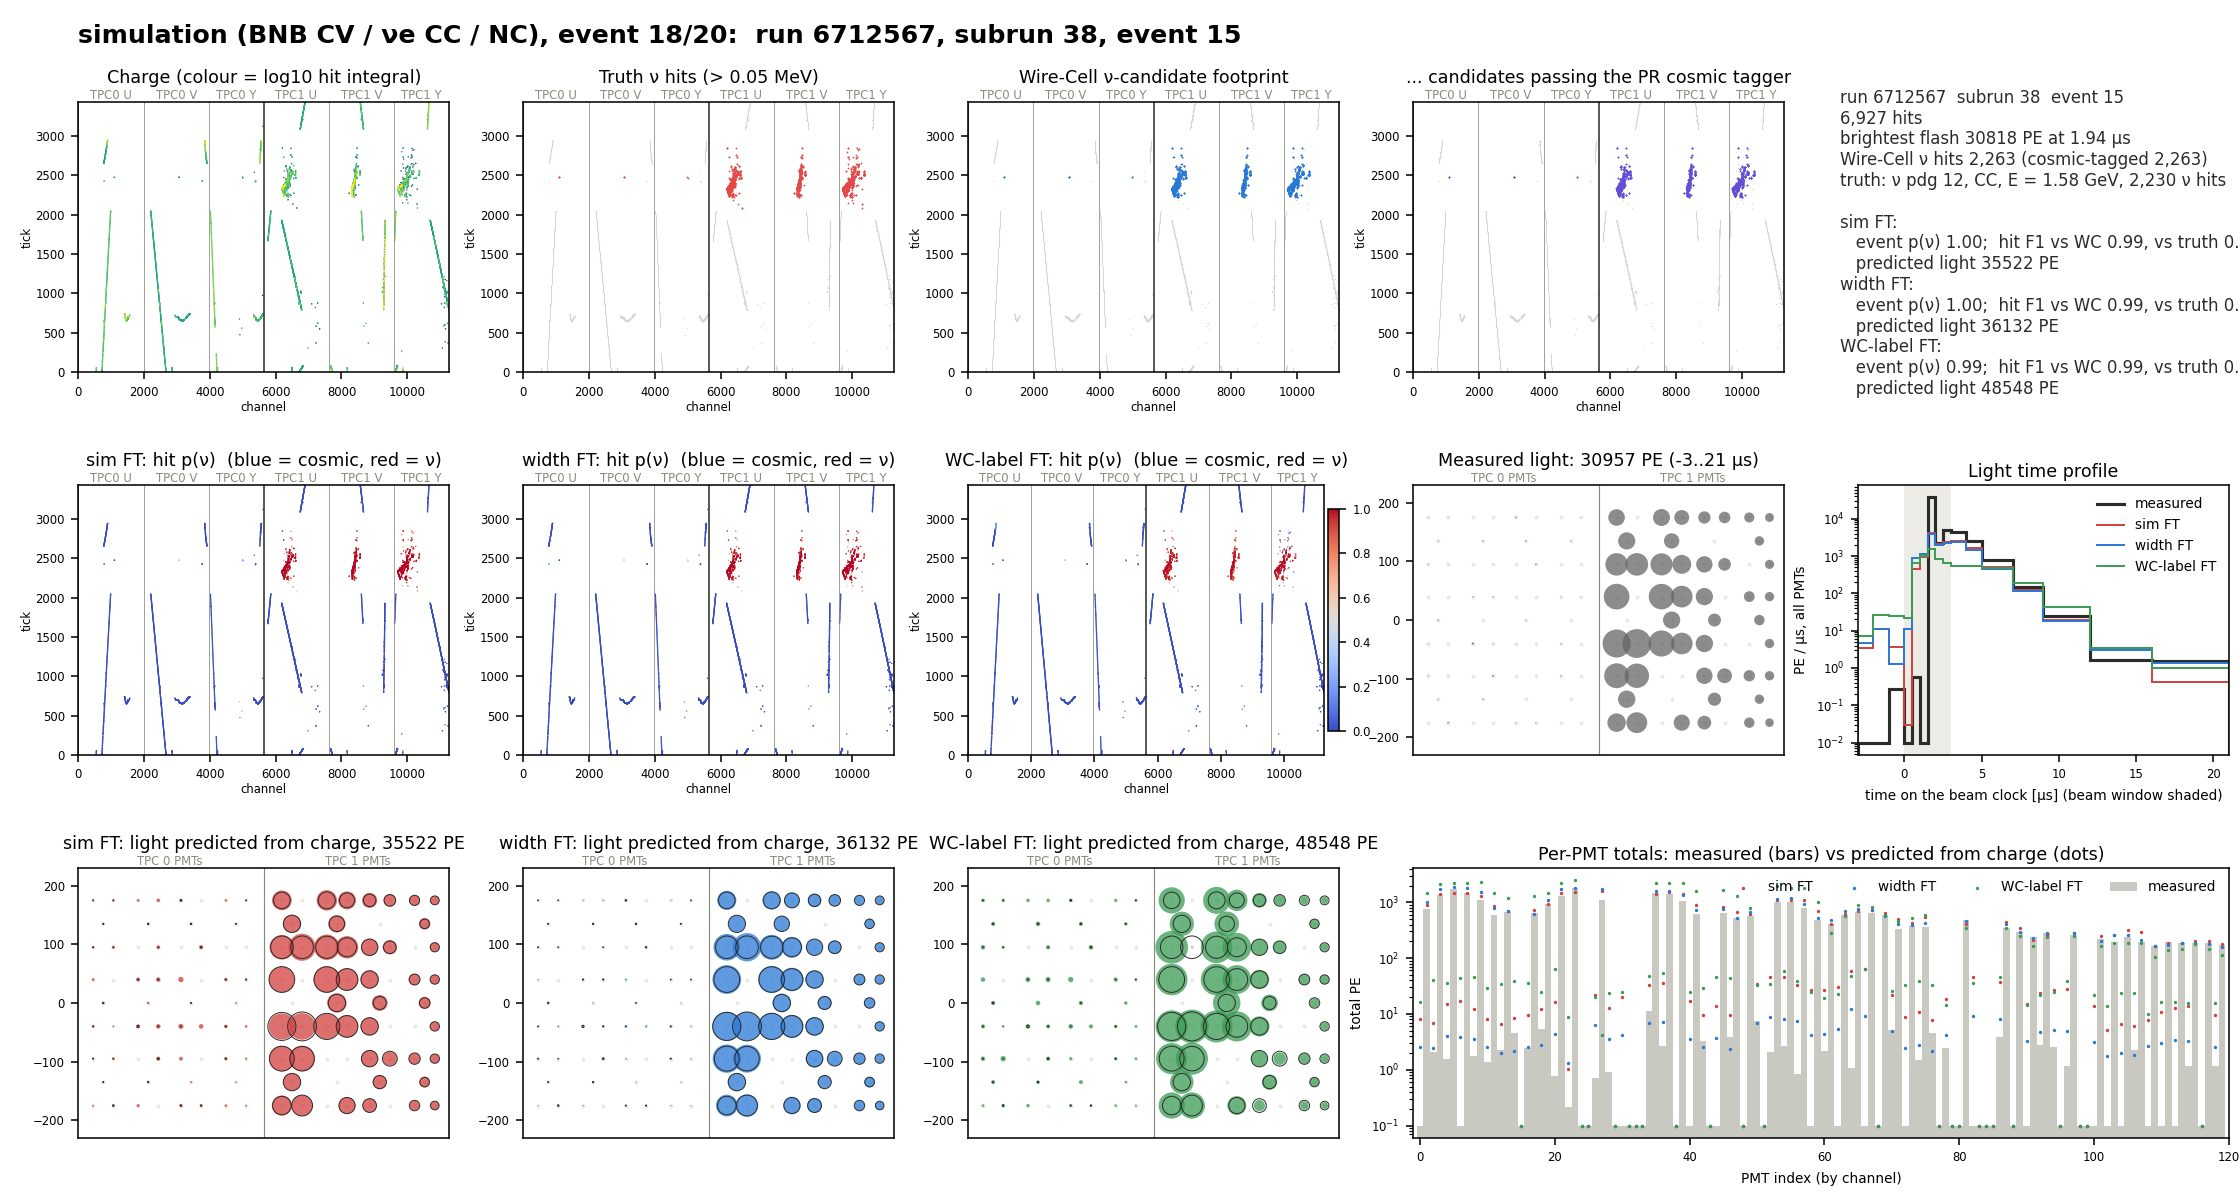
\includegraphics[width=\paperwidth,height=\paperheight,keepaspectratio]{displays/sim_17.jpg}}
\end{frame}
% Simulation 19/20: run 6703266, subrun 87, event 83; event p(nu): sim FT 0.74, width FT 0.51, WC-label FT 0.99
\begin{frame}[plain]
  \centering\vspace*{-2pt}
  \makebox[\linewidth][c]{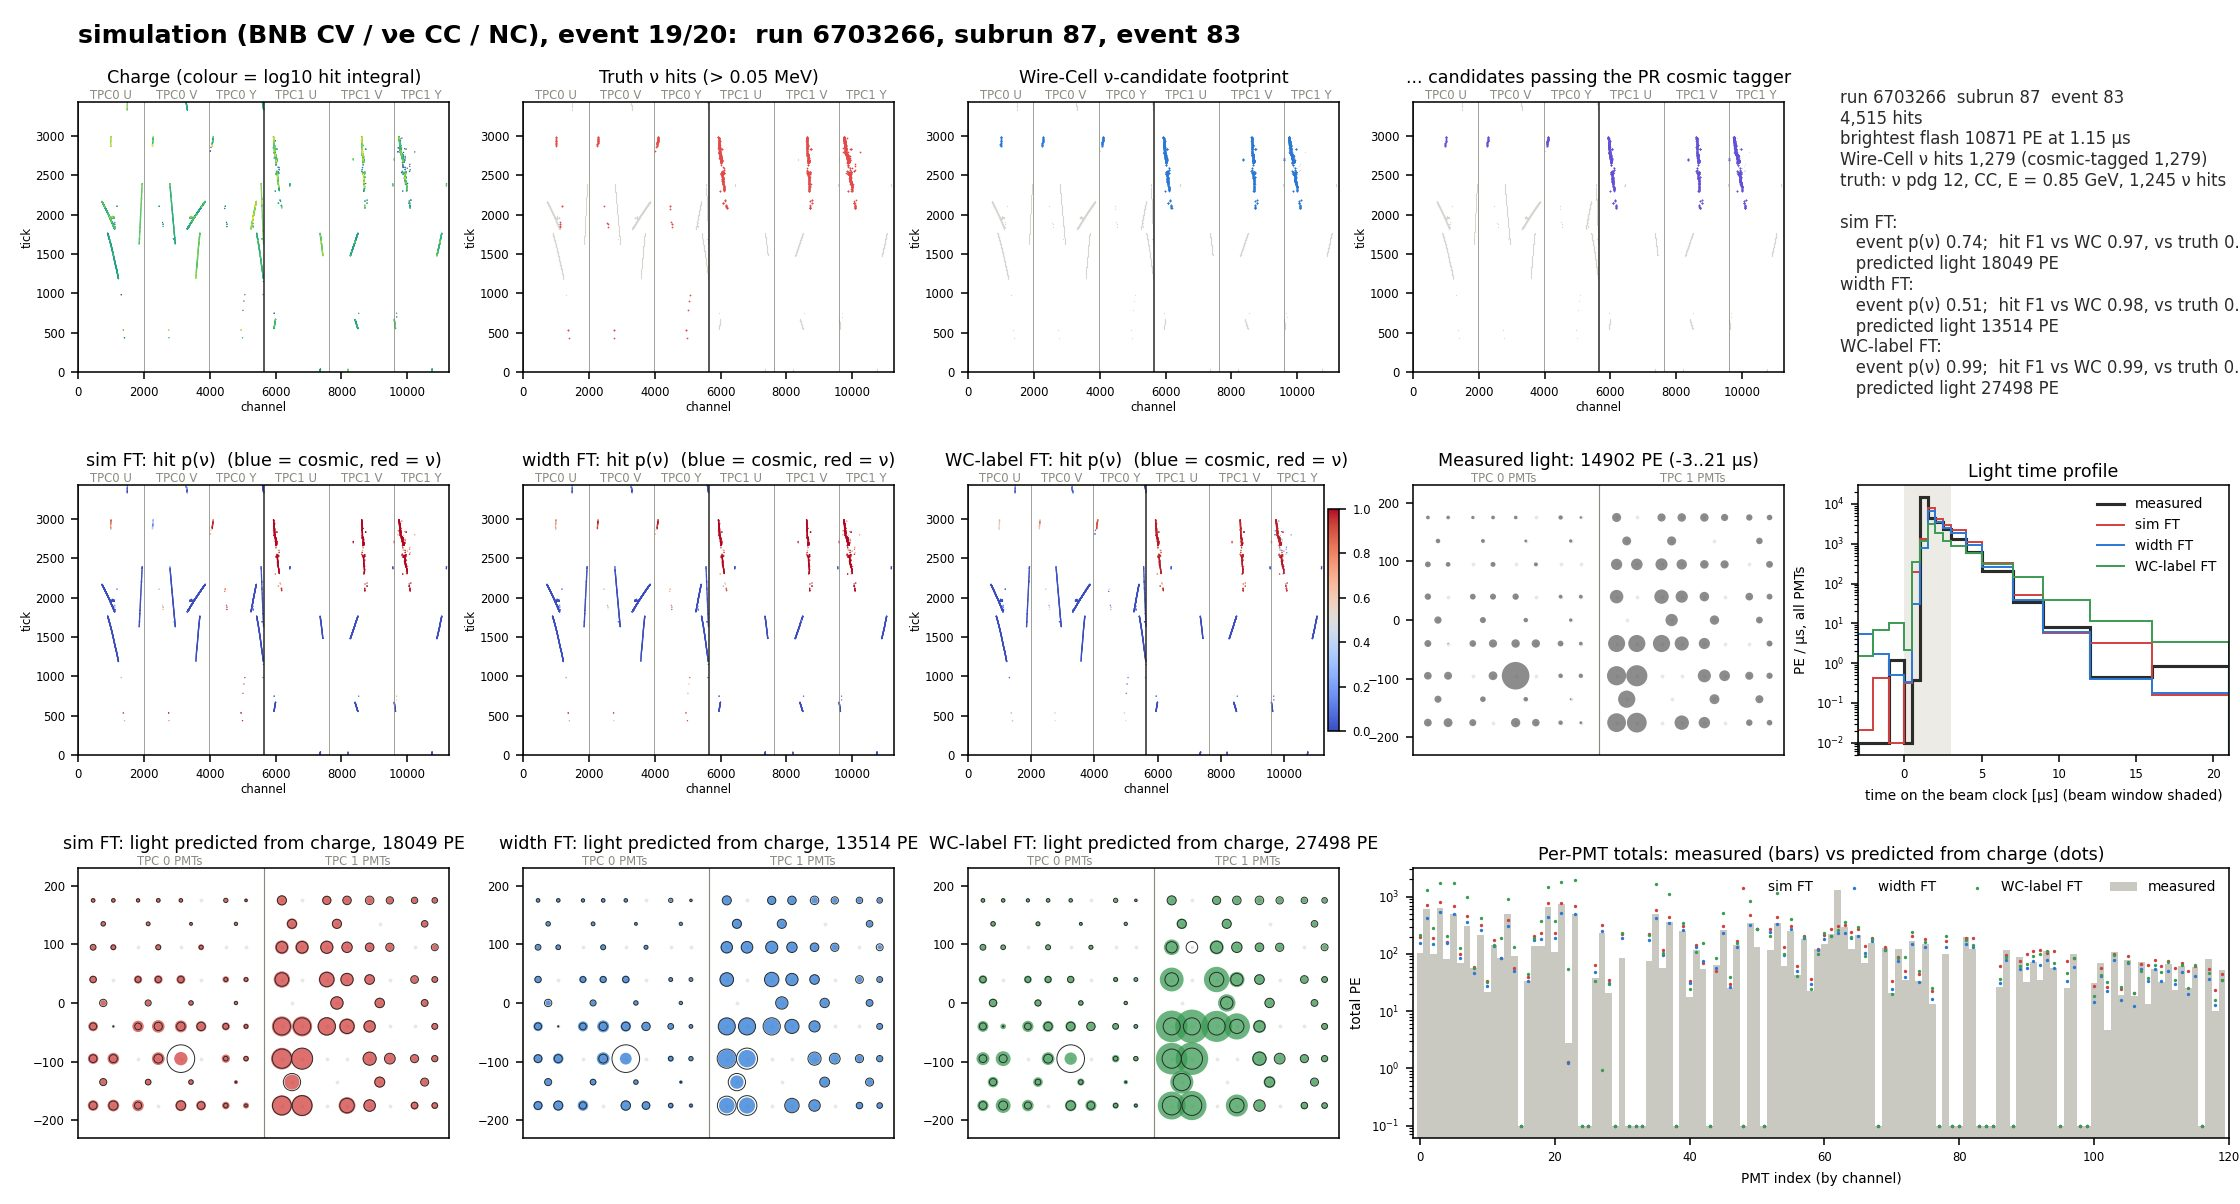
\includegraphics[width=\paperwidth,height=\paperheight,keepaspectratio]{displays/sim_18.jpg}}
\end{frame}
% Simulation 20/20: run 7022028, subrun 0, event 121; event p(nu): sim FT 1.00, width FT 1.00, WC-label FT 0.81
\begin{frame}[plain]
  \centering\vspace*{-2pt}
  \makebox[\linewidth][c]{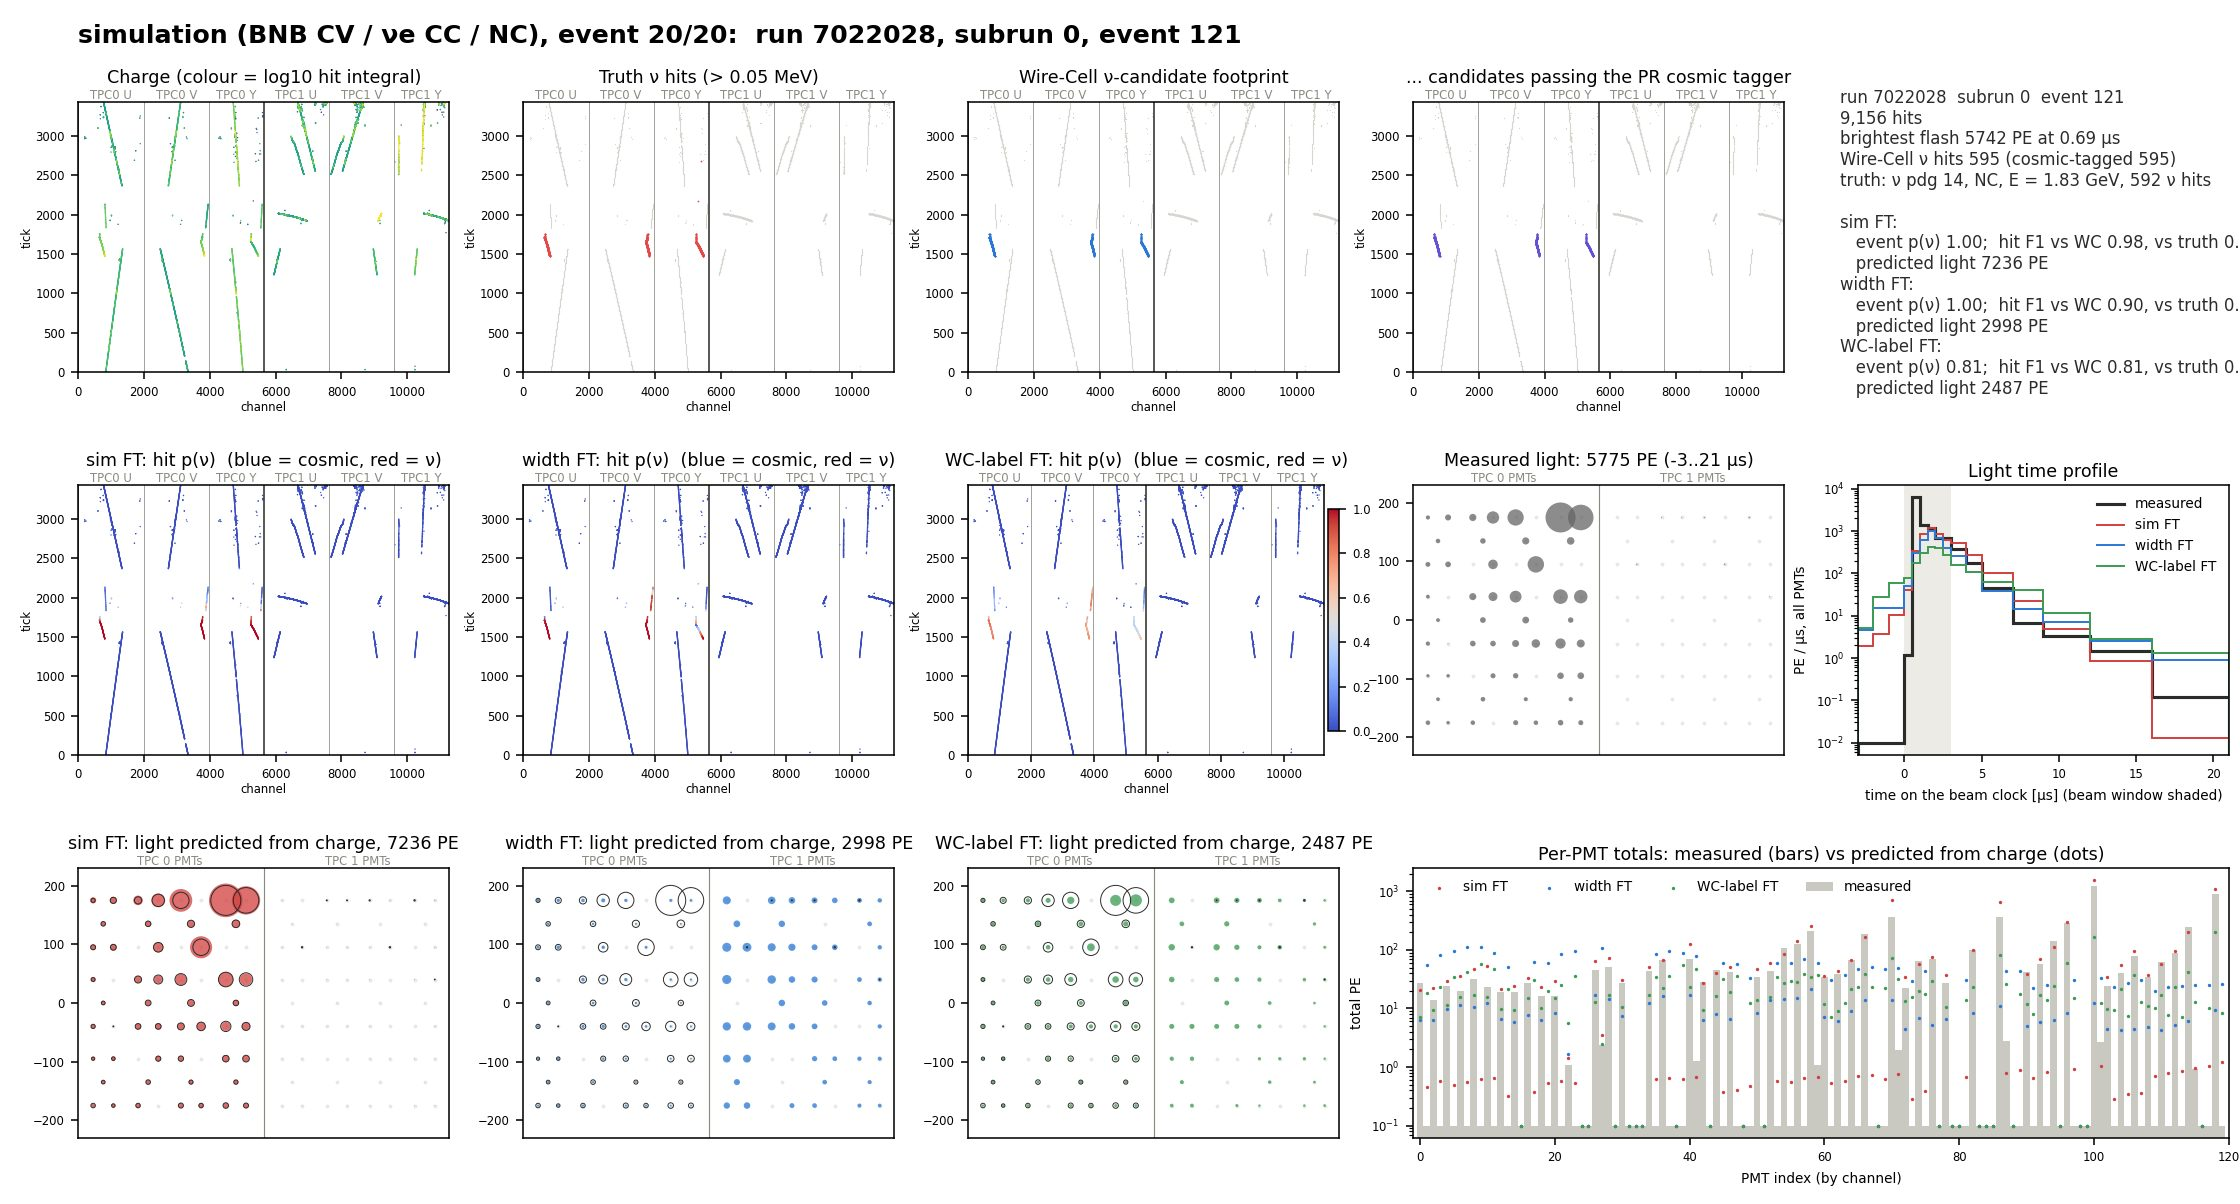
\includegraphics[width=\paperwidth,height=\paperheight,keepaspectratio]{displays/sim_19.jpg}}
\end{frame}
\subsection{Beam-on data}
% Beam-on data 1/20: run 18255, subrun 1, event 212212; event p(nu): sim FT 0.00, width FT 0.00, WC-label FT 0.00
\begin{frame}[plain]
  \centering\vspace*{-2pt}
  \makebox[\linewidth][c]{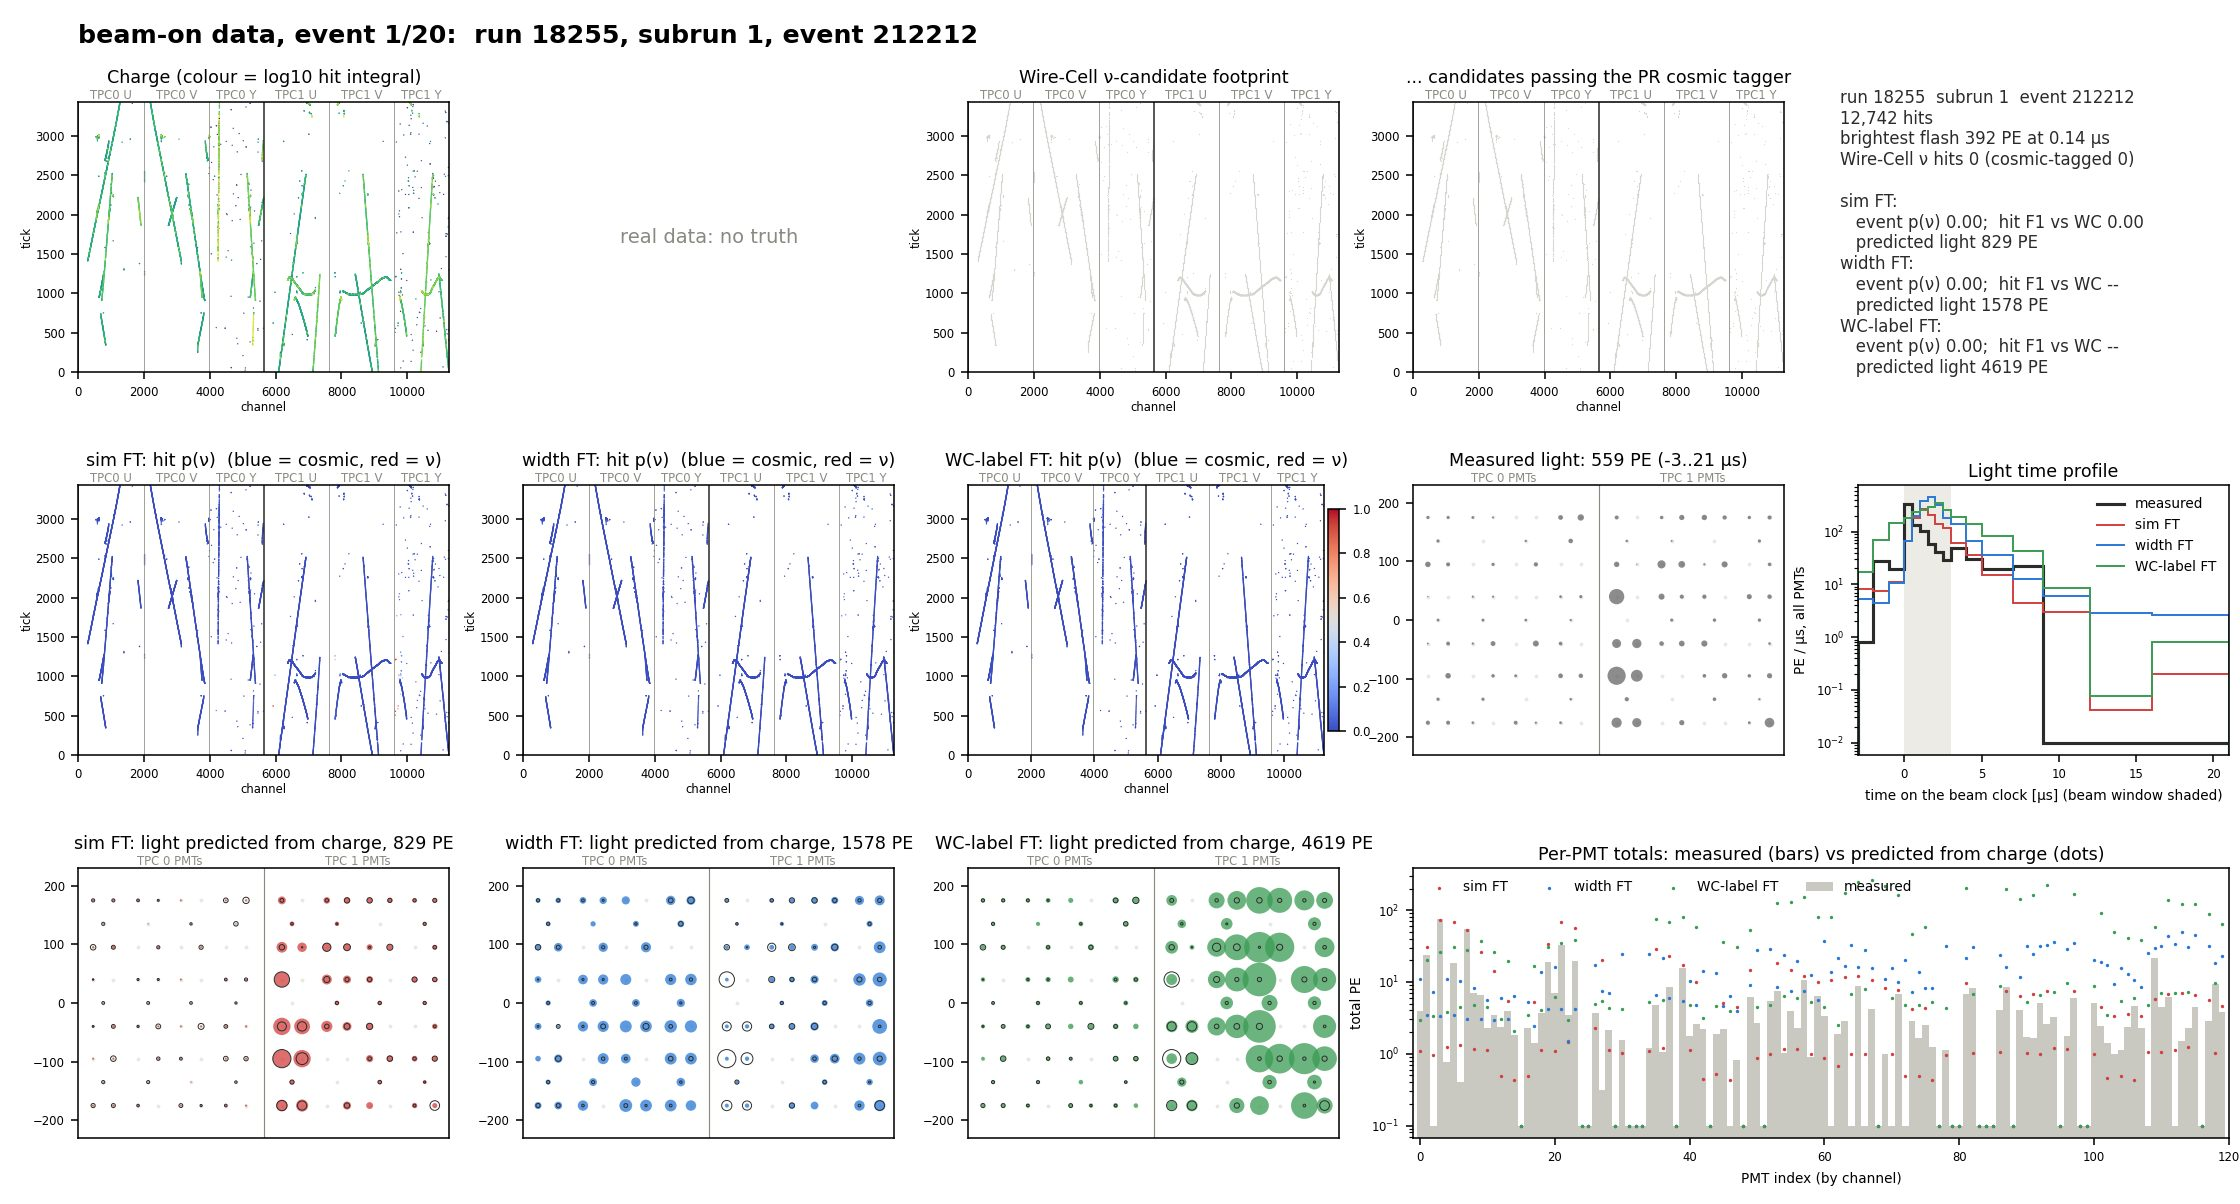
\includegraphics[width=\paperwidth,height=\paperheight,keepaspectratio]{displays/on_00.jpg}}
\end{frame}
% Beam-on data 2/20: run 18255, subrun 1, event 104444; event p(nu): sim FT 0.00, width FT 0.00, WC-label FT 0.90
\begin{frame}[plain]
  \centering\vspace*{-2pt}
  \makebox[\linewidth][c]{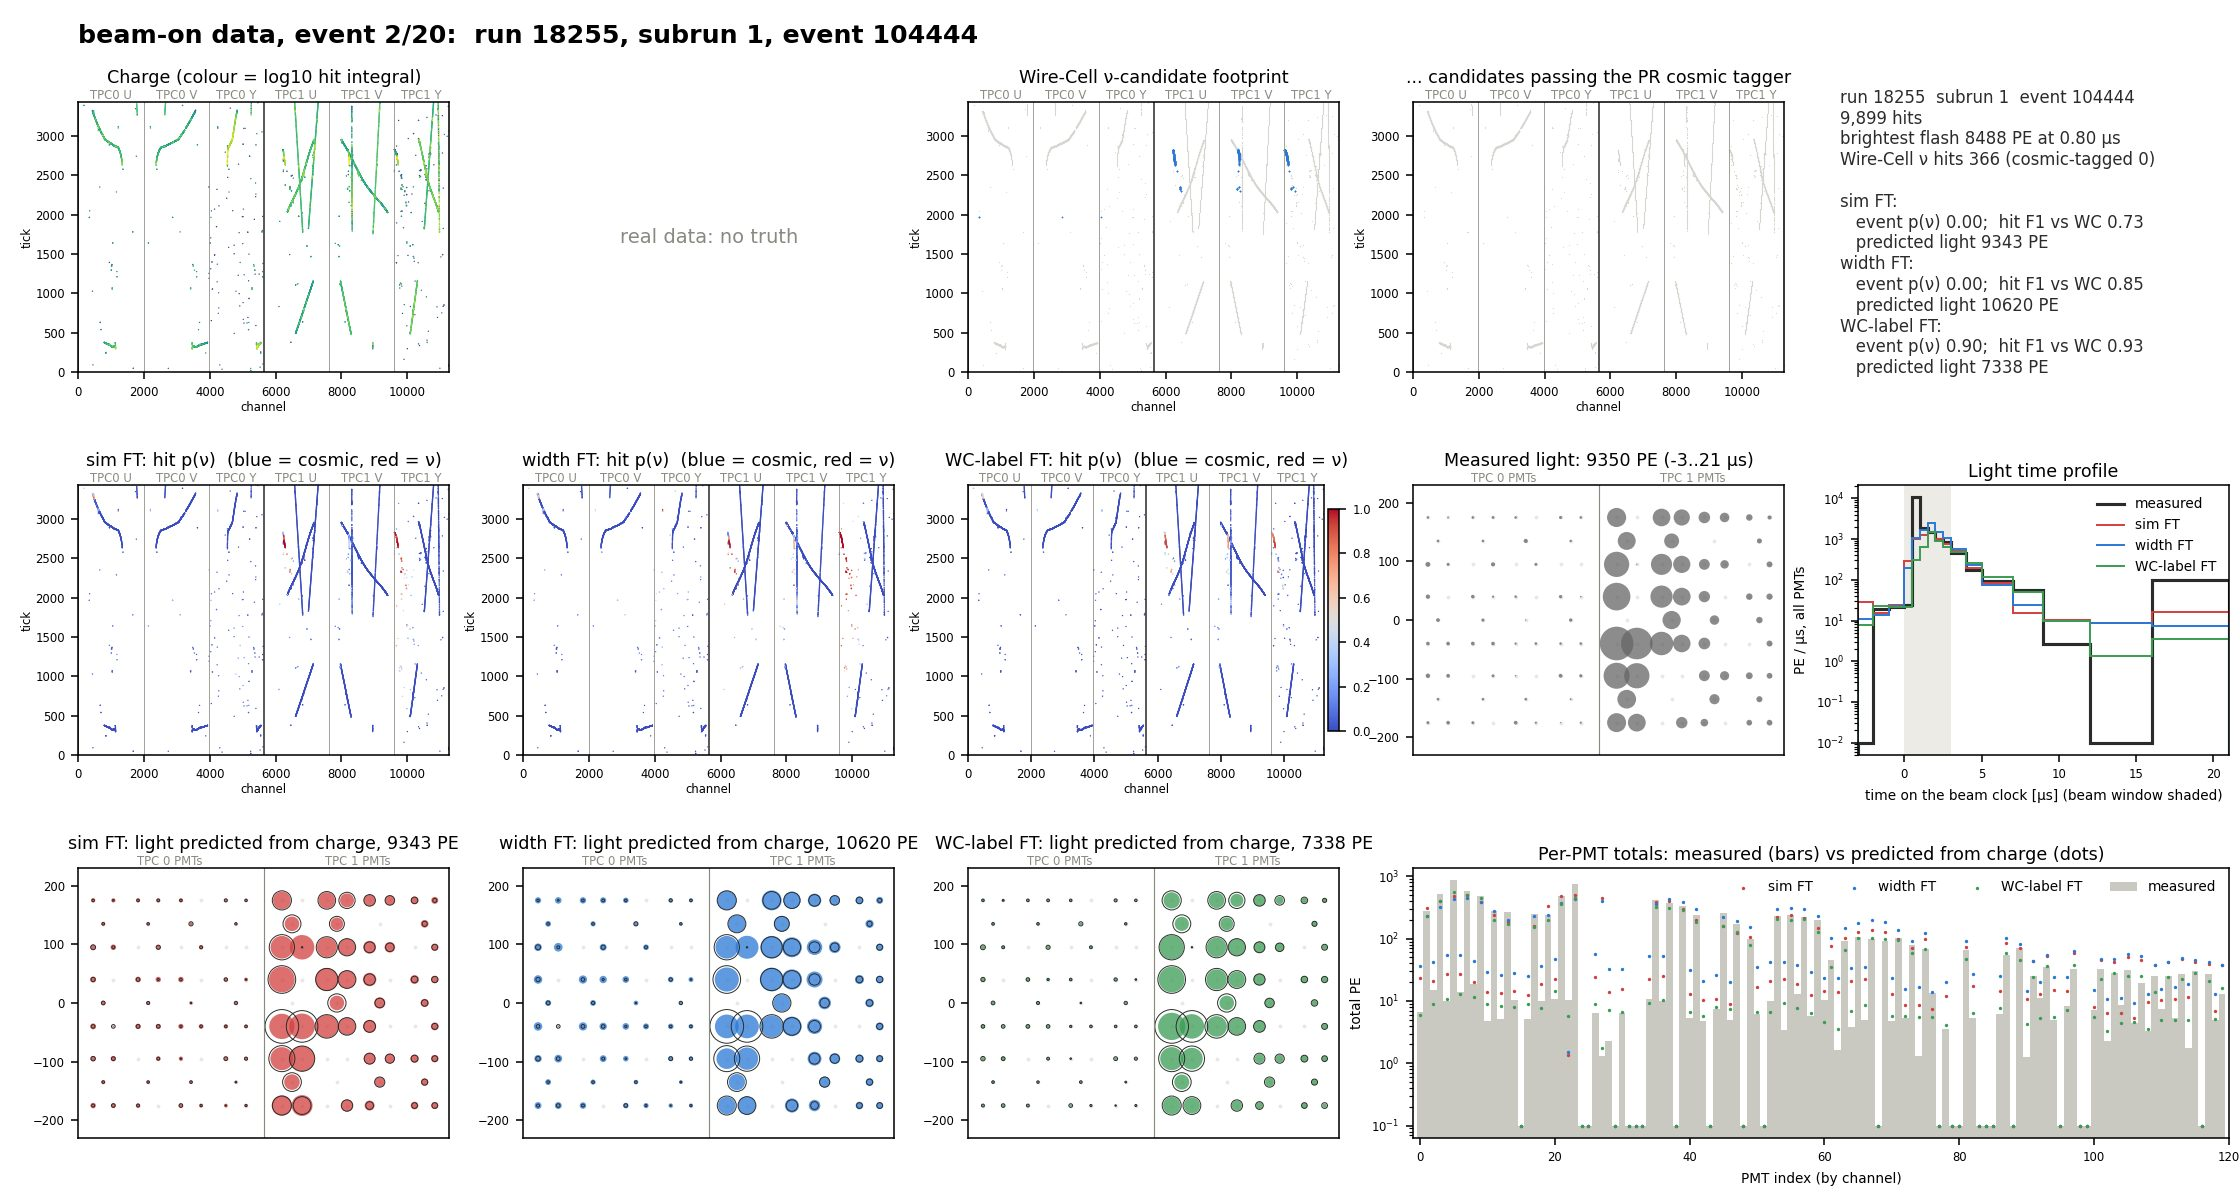
\includegraphics[width=\paperwidth,height=\paperheight,keepaspectratio]{displays/on_01.jpg}}
\end{frame}
% Beam-on data 3/20: run 18255, subrun 1, event 225882; event p(nu): sim FT 0.00, width FT 0.00, WC-label FT 0.34
\begin{frame}[plain]
  \centering\vspace*{-2pt}
  \makebox[\linewidth][c]{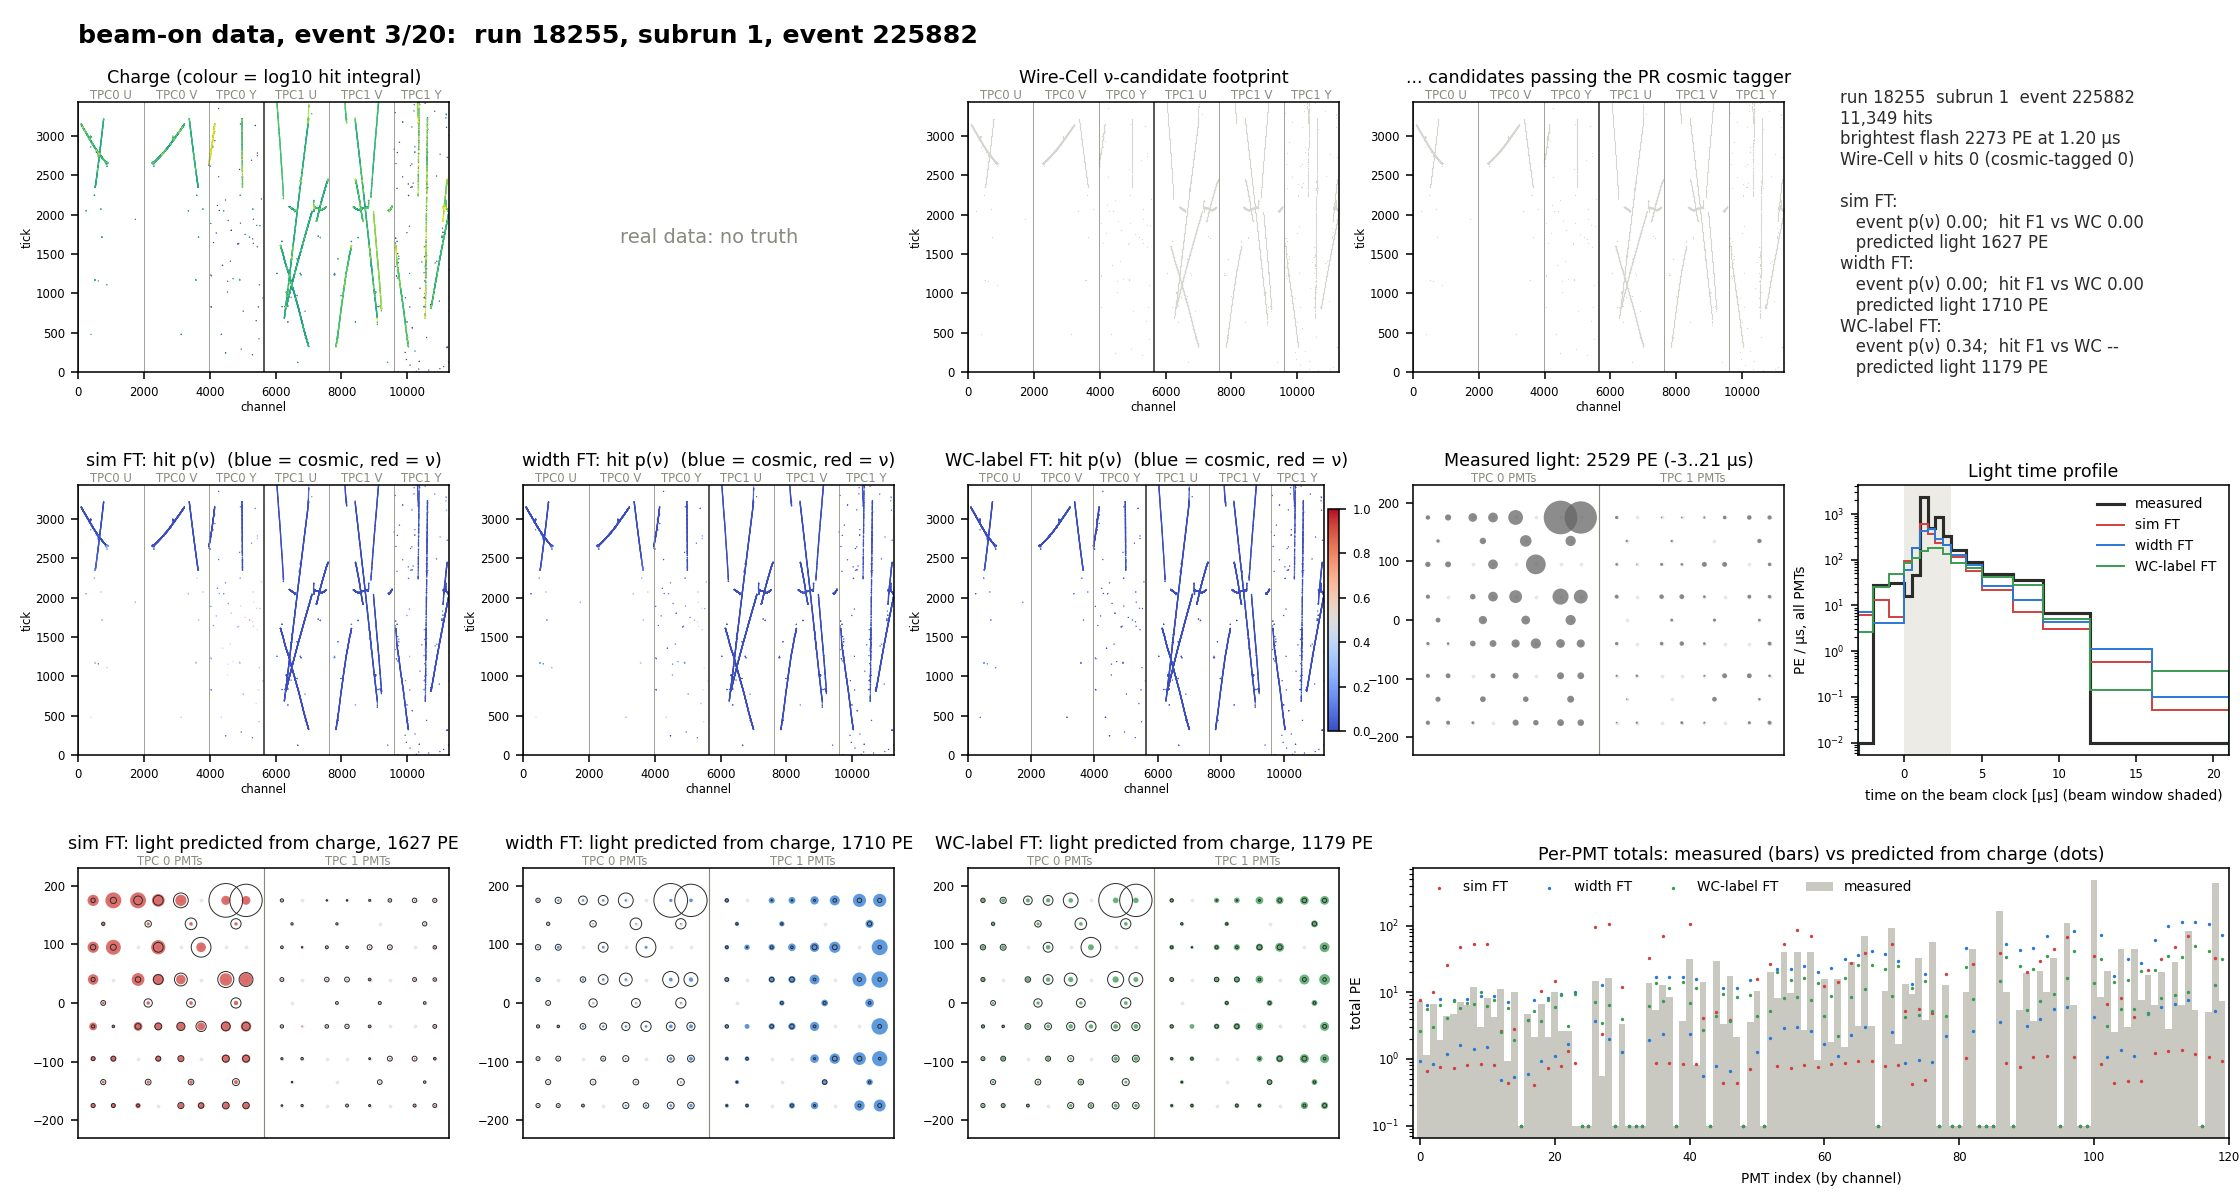
\includegraphics[width=\paperwidth,height=\paperheight,keepaspectratio]{displays/on_02.jpg}}
\end{frame}
% Beam-on data 4/20: run 18255, subrun 1, event 513616; event p(nu): sim FT 0.00, width FT 0.00, WC-label FT 0.04
\begin{frame}[plain]
  \centering\vspace*{-2pt}
  \makebox[\linewidth][c]{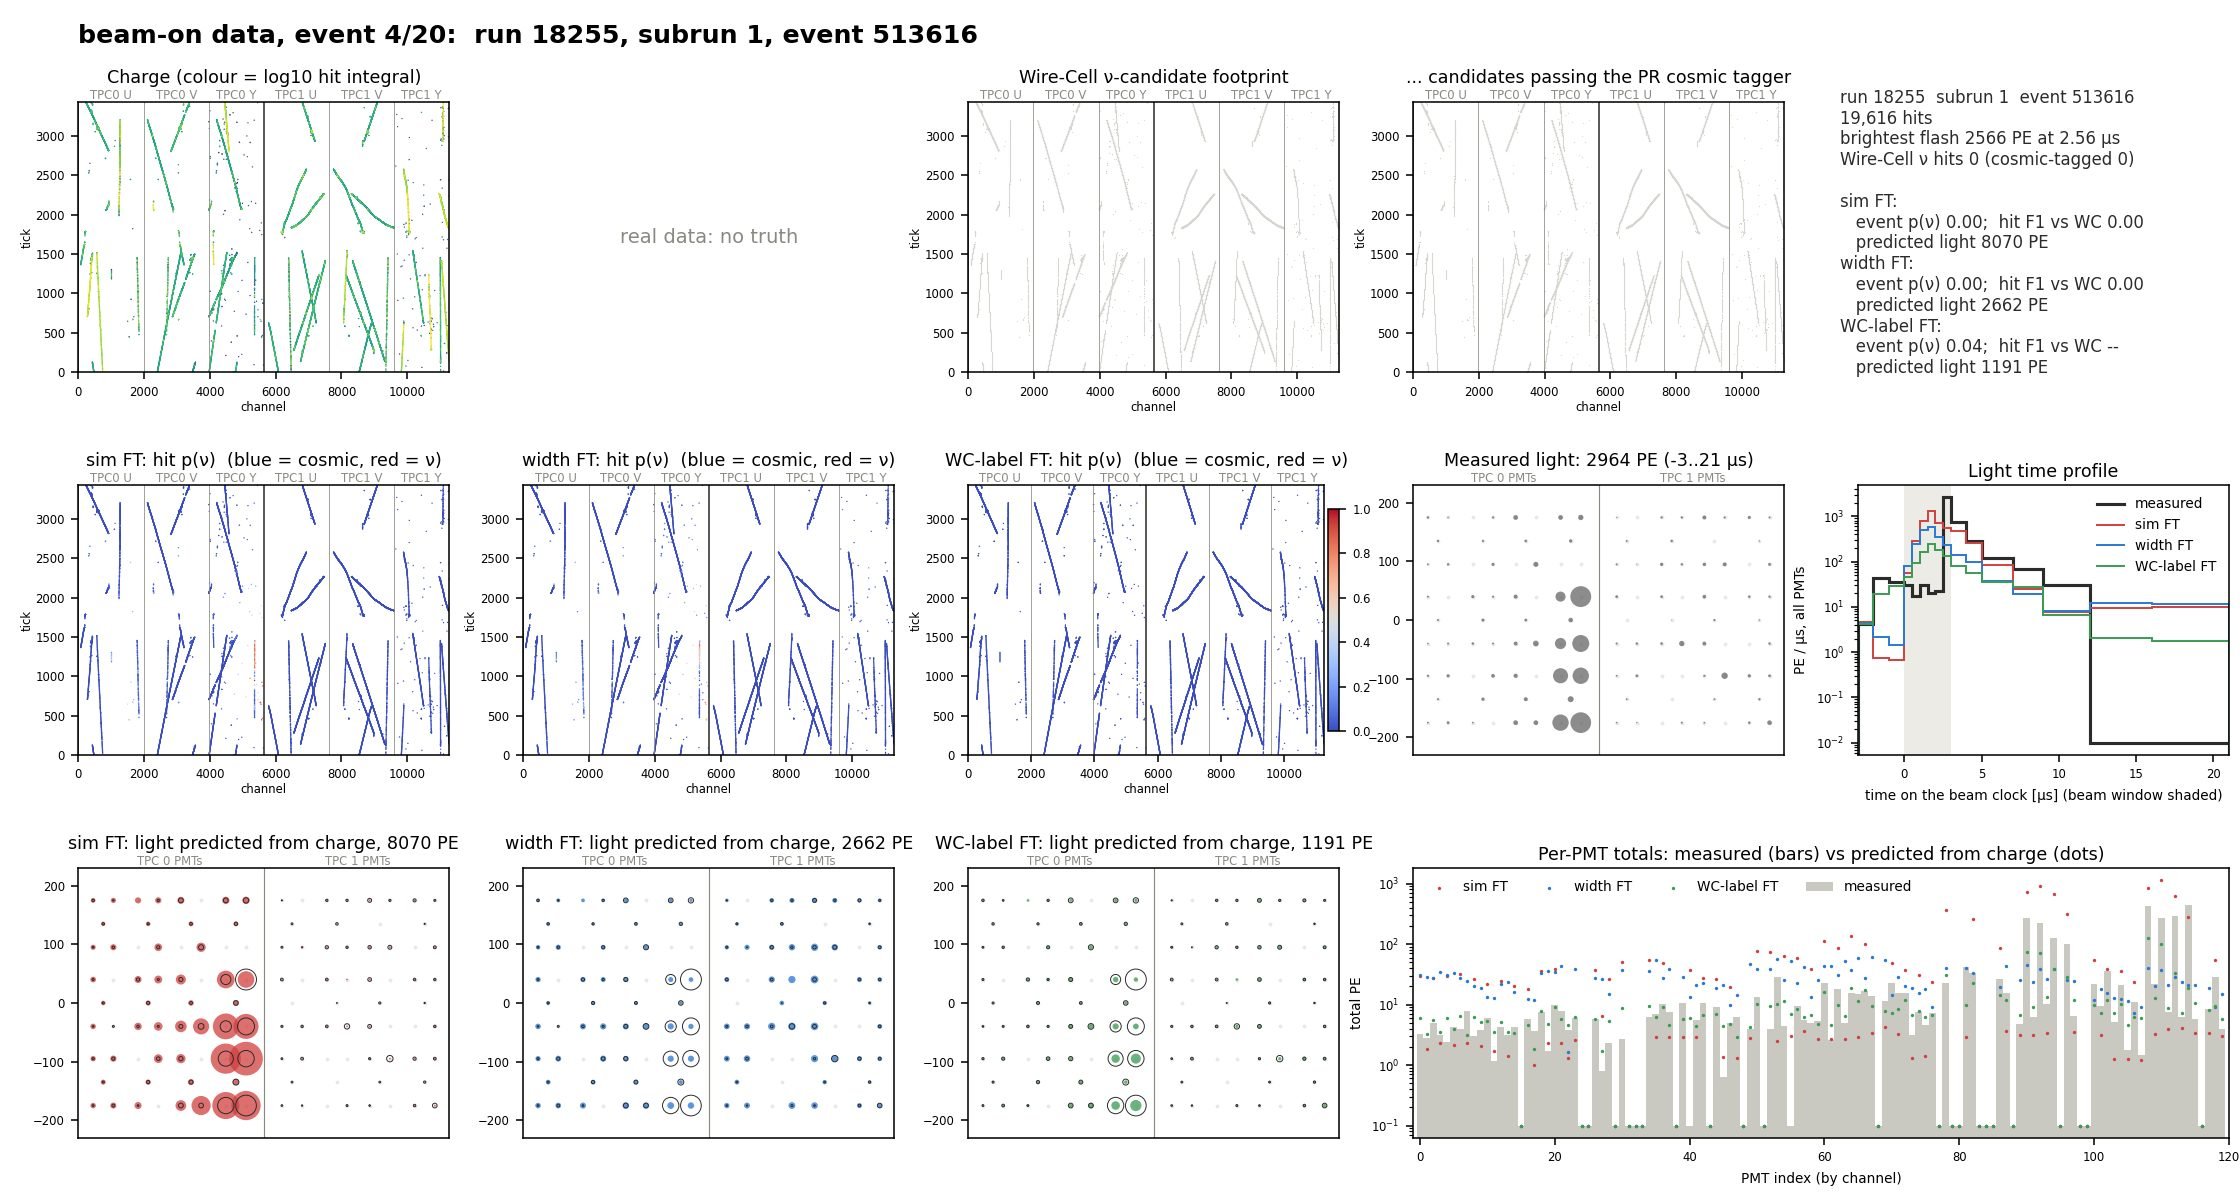
\includegraphics[width=\paperwidth,height=\paperheight,keepaspectratio]{displays/on_03.jpg}}
\end{frame}
% Beam-on data 5/20: run 18255, subrun 1, event 272264; event p(nu): sim FT 1.00, width FT 1.00, WC-label FT 0.96
\begin{frame}[plain]
  \centering\vspace*{-2pt}
  \makebox[\linewidth][c]{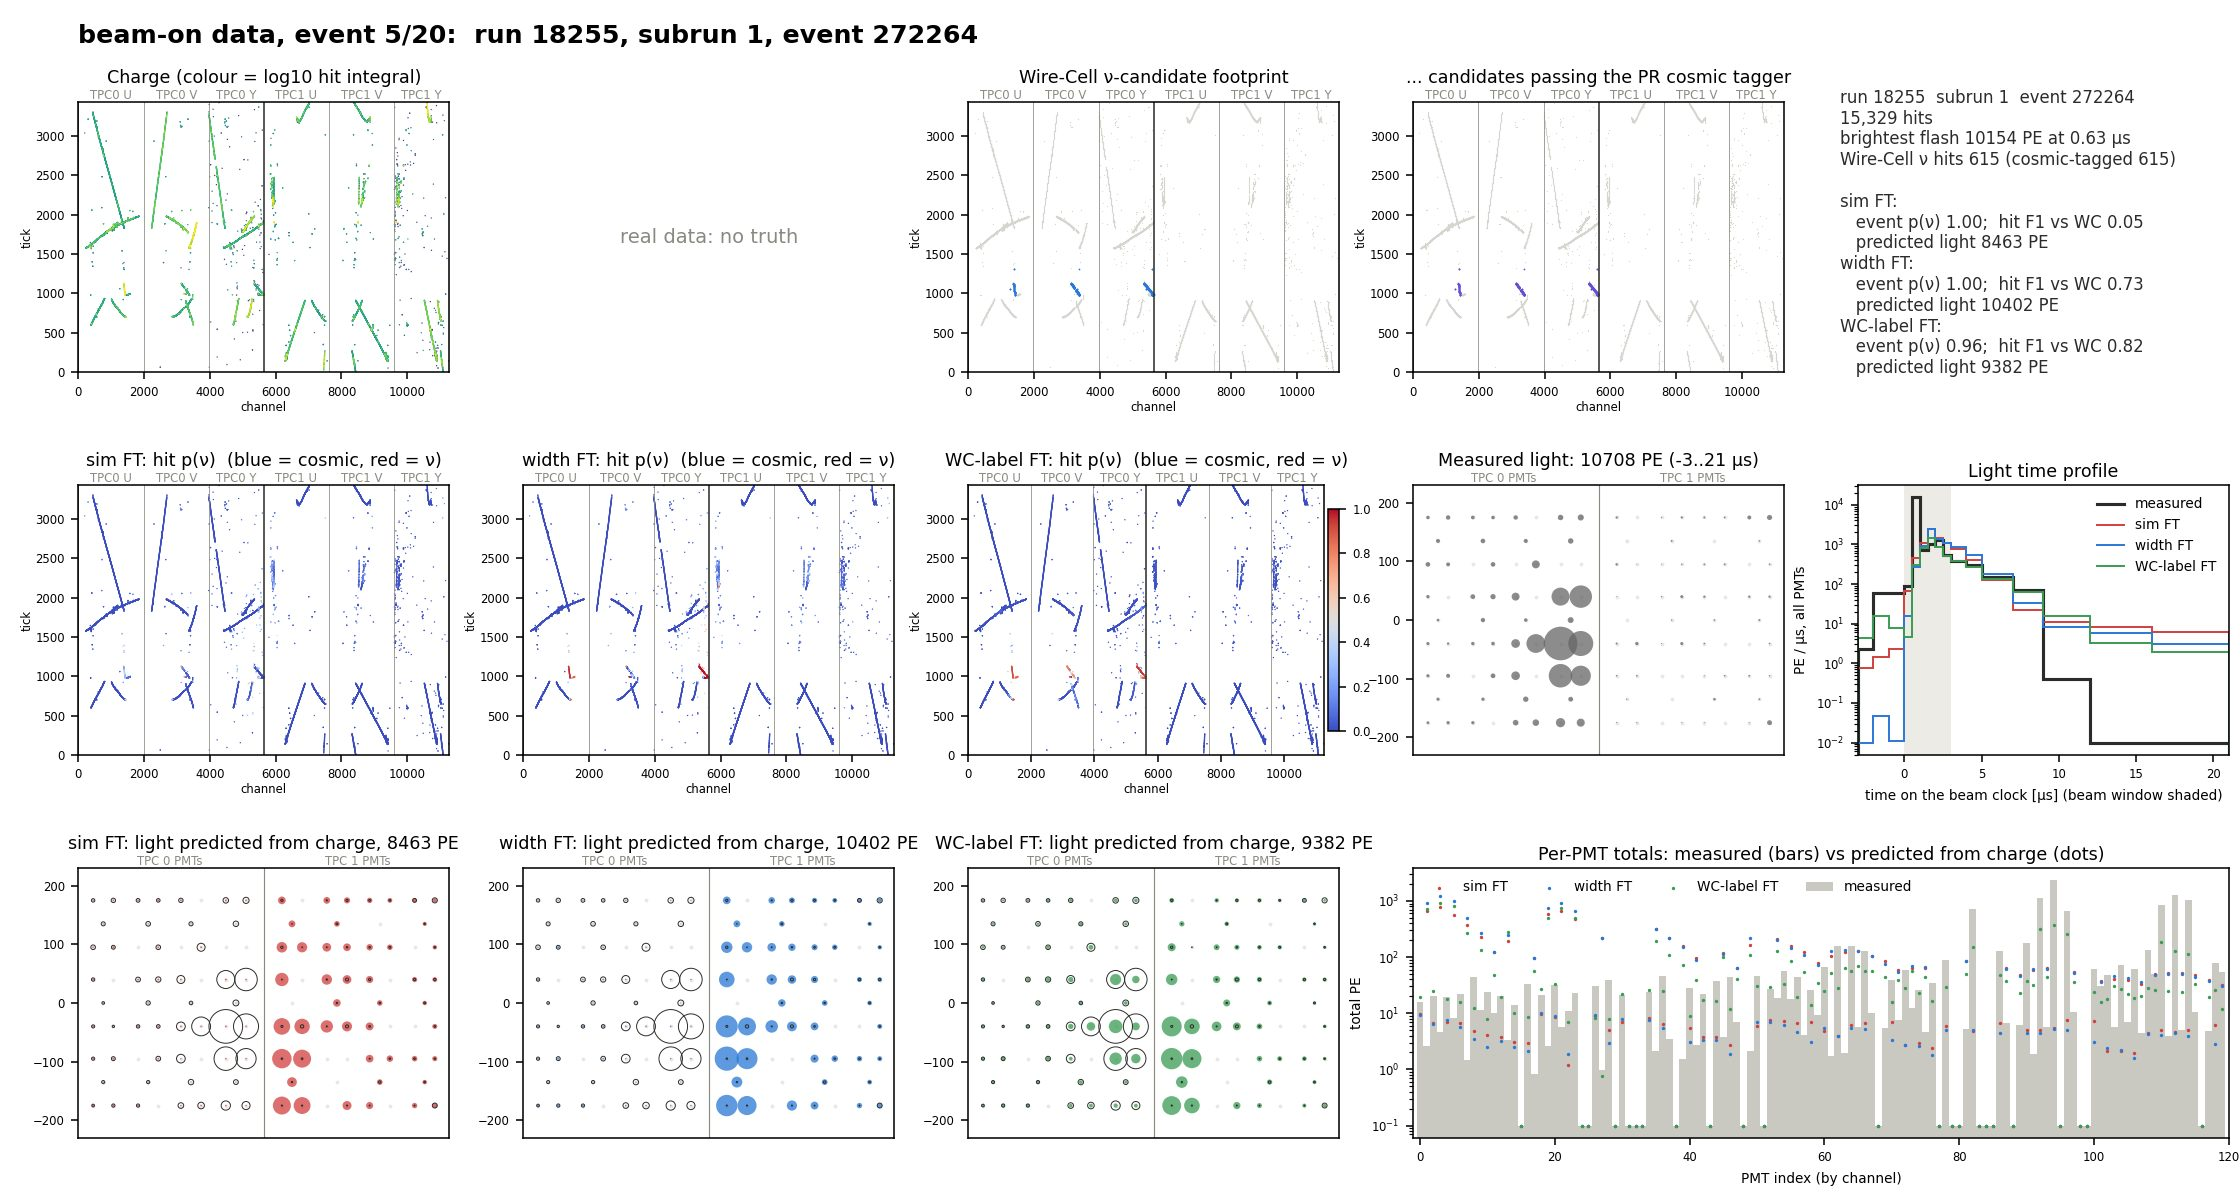
\includegraphics[width=\paperwidth,height=\paperheight,keepaspectratio]{displays/on_04.jpg}}
\end{frame}
% Beam-on data 6/20: run 18255, subrun 1, event 447683; event p(nu): sim FT 0.00, width FT 0.00, WC-label FT 0.84
\begin{frame}[plain]
  \centering\vspace*{-2pt}
  \makebox[\linewidth][c]{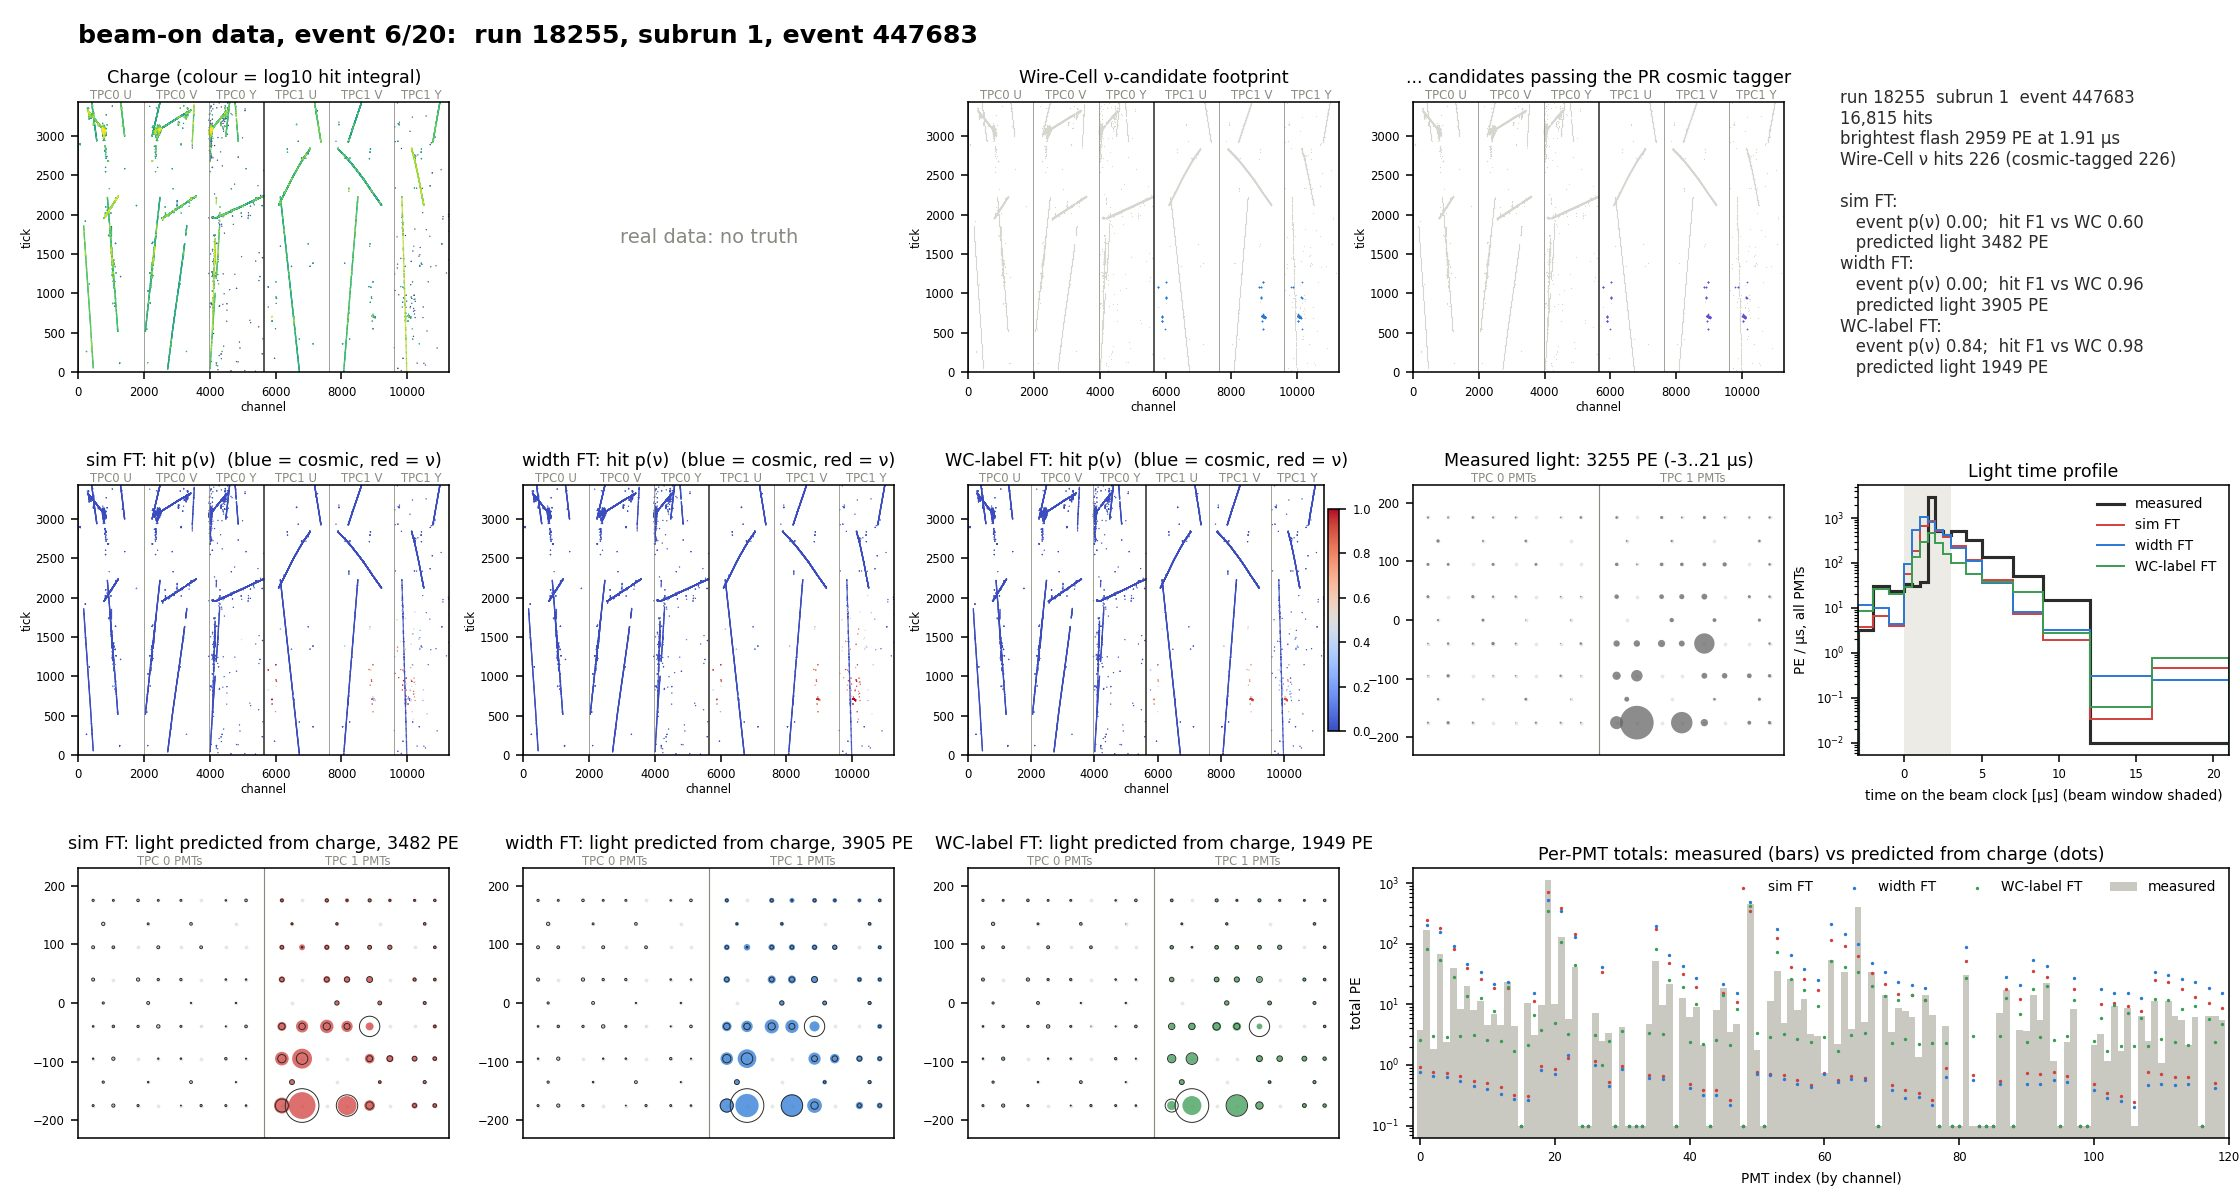
\includegraphics[width=\paperwidth,height=\paperheight,keepaspectratio]{displays/on_05.jpg}}
\end{frame}
% Beam-on data 7/20: run 18259, subrun 1, event 255438; event p(nu): sim FT 1.00, width FT 1.00, WC-label FT 0.97
\begin{frame}[plain]
  \centering\vspace*{-2pt}
  \makebox[\linewidth][c]{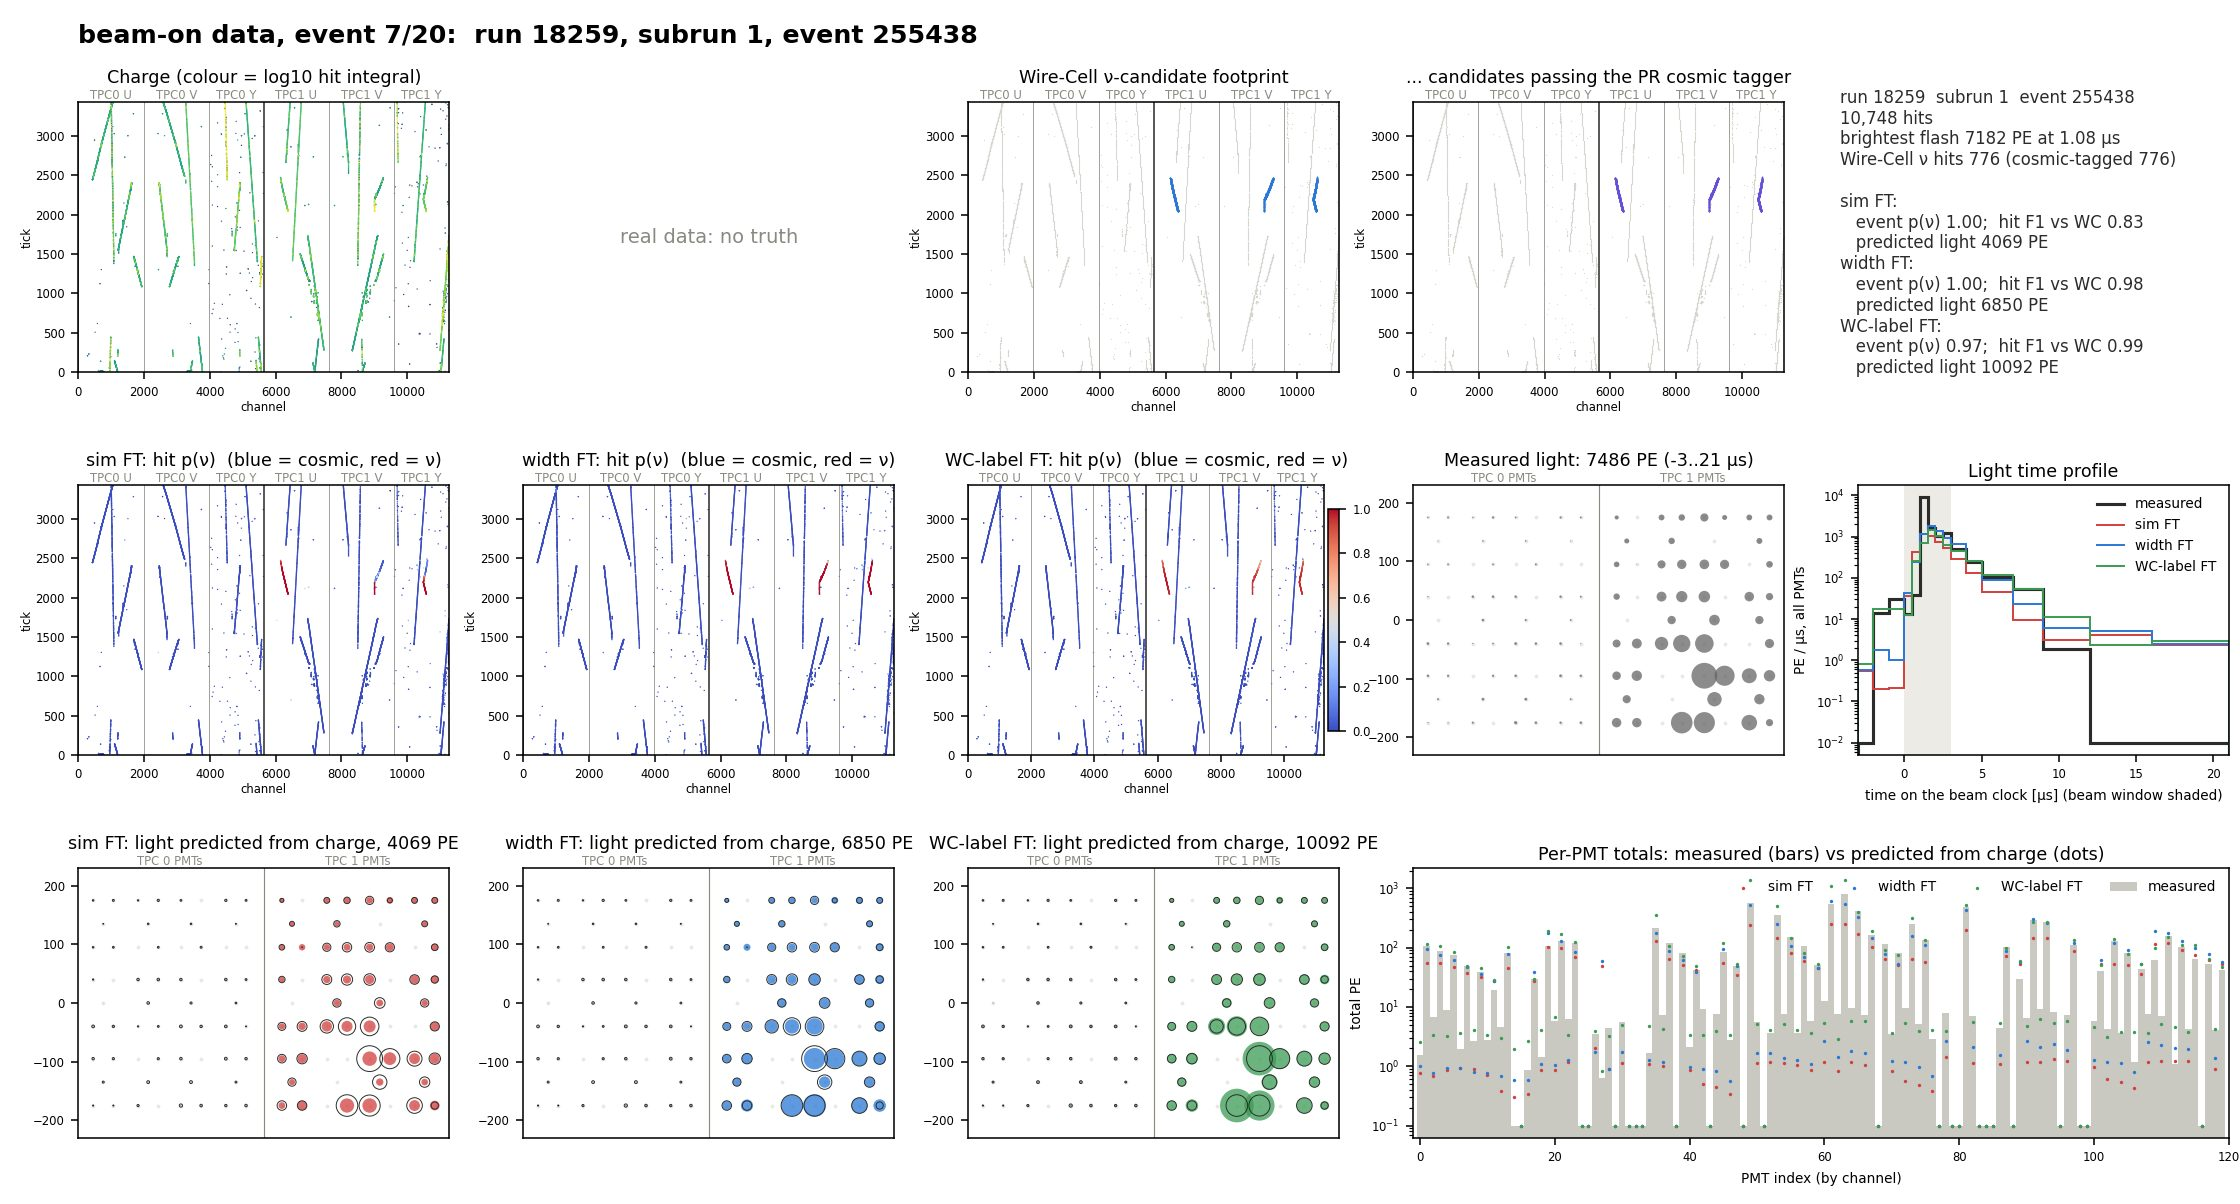
\includegraphics[width=\paperwidth,height=\paperheight,keepaspectratio]{displays/on_06.jpg}}
\end{frame}
% Beam-on data 8/20: run 18255, subrun 1, event 486168; event p(nu): sim FT 0.99, width FT 1.00, WC-label FT 0.93
\begin{frame}[plain]
  \centering\vspace*{-2pt}
  \makebox[\linewidth][c]{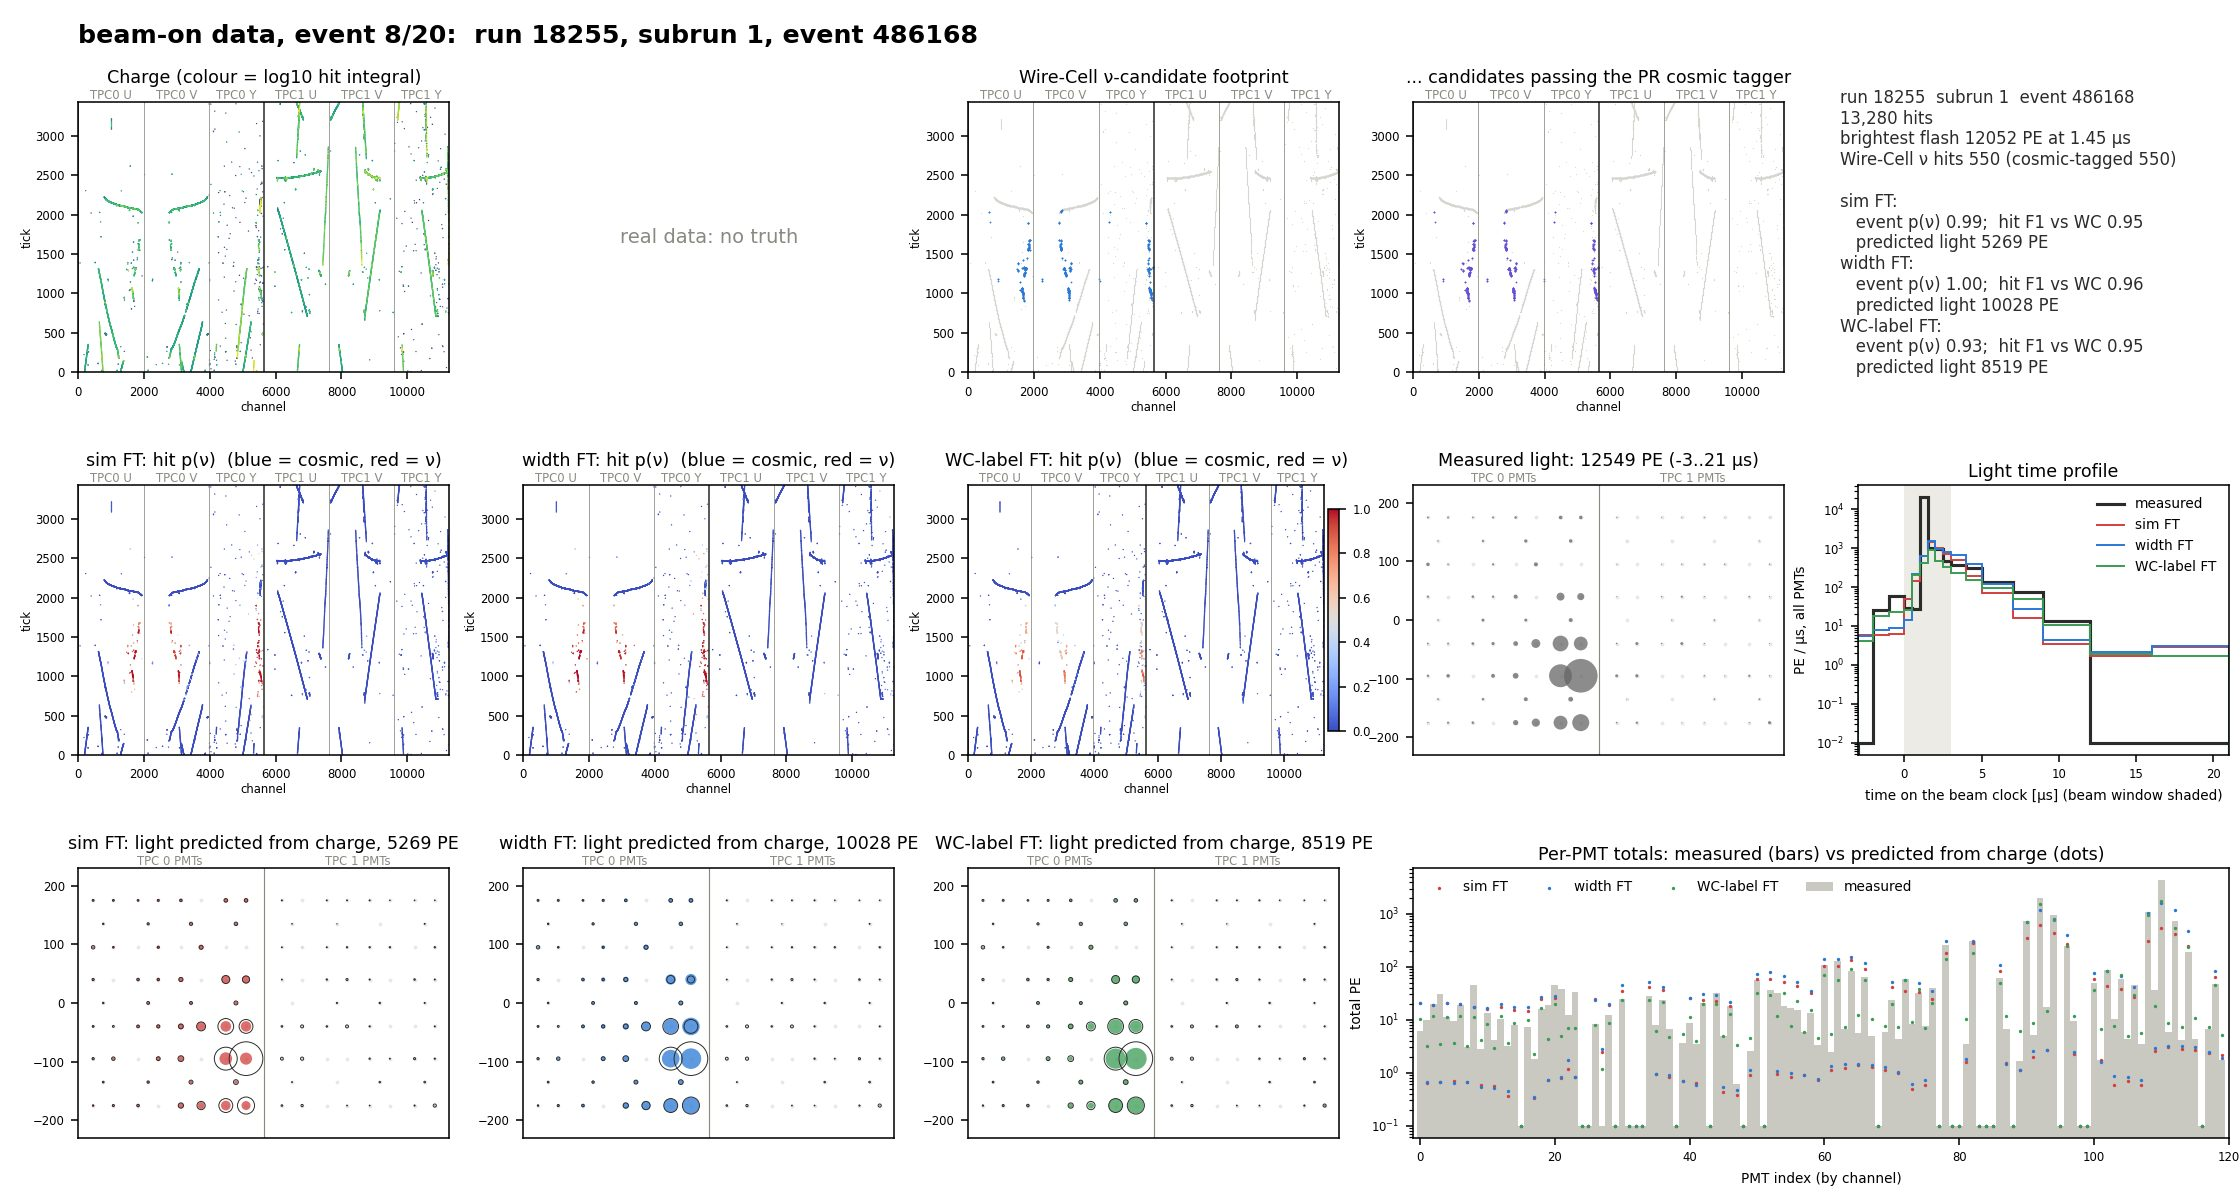
\includegraphics[width=\paperwidth,height=\paperheight,keepaspectratio]{displays/on_07.jpg}}
\end{frame}
% Beam-on data 9/20: run 18255, subrun 1, event 28768; event p(nu): sim FT 0.00, width FT 0.00, WC-label FT 0.08
\begin{frame}[plain]
  \centering\vspace*{-2pt}
  \makebox[\linewidth][c]{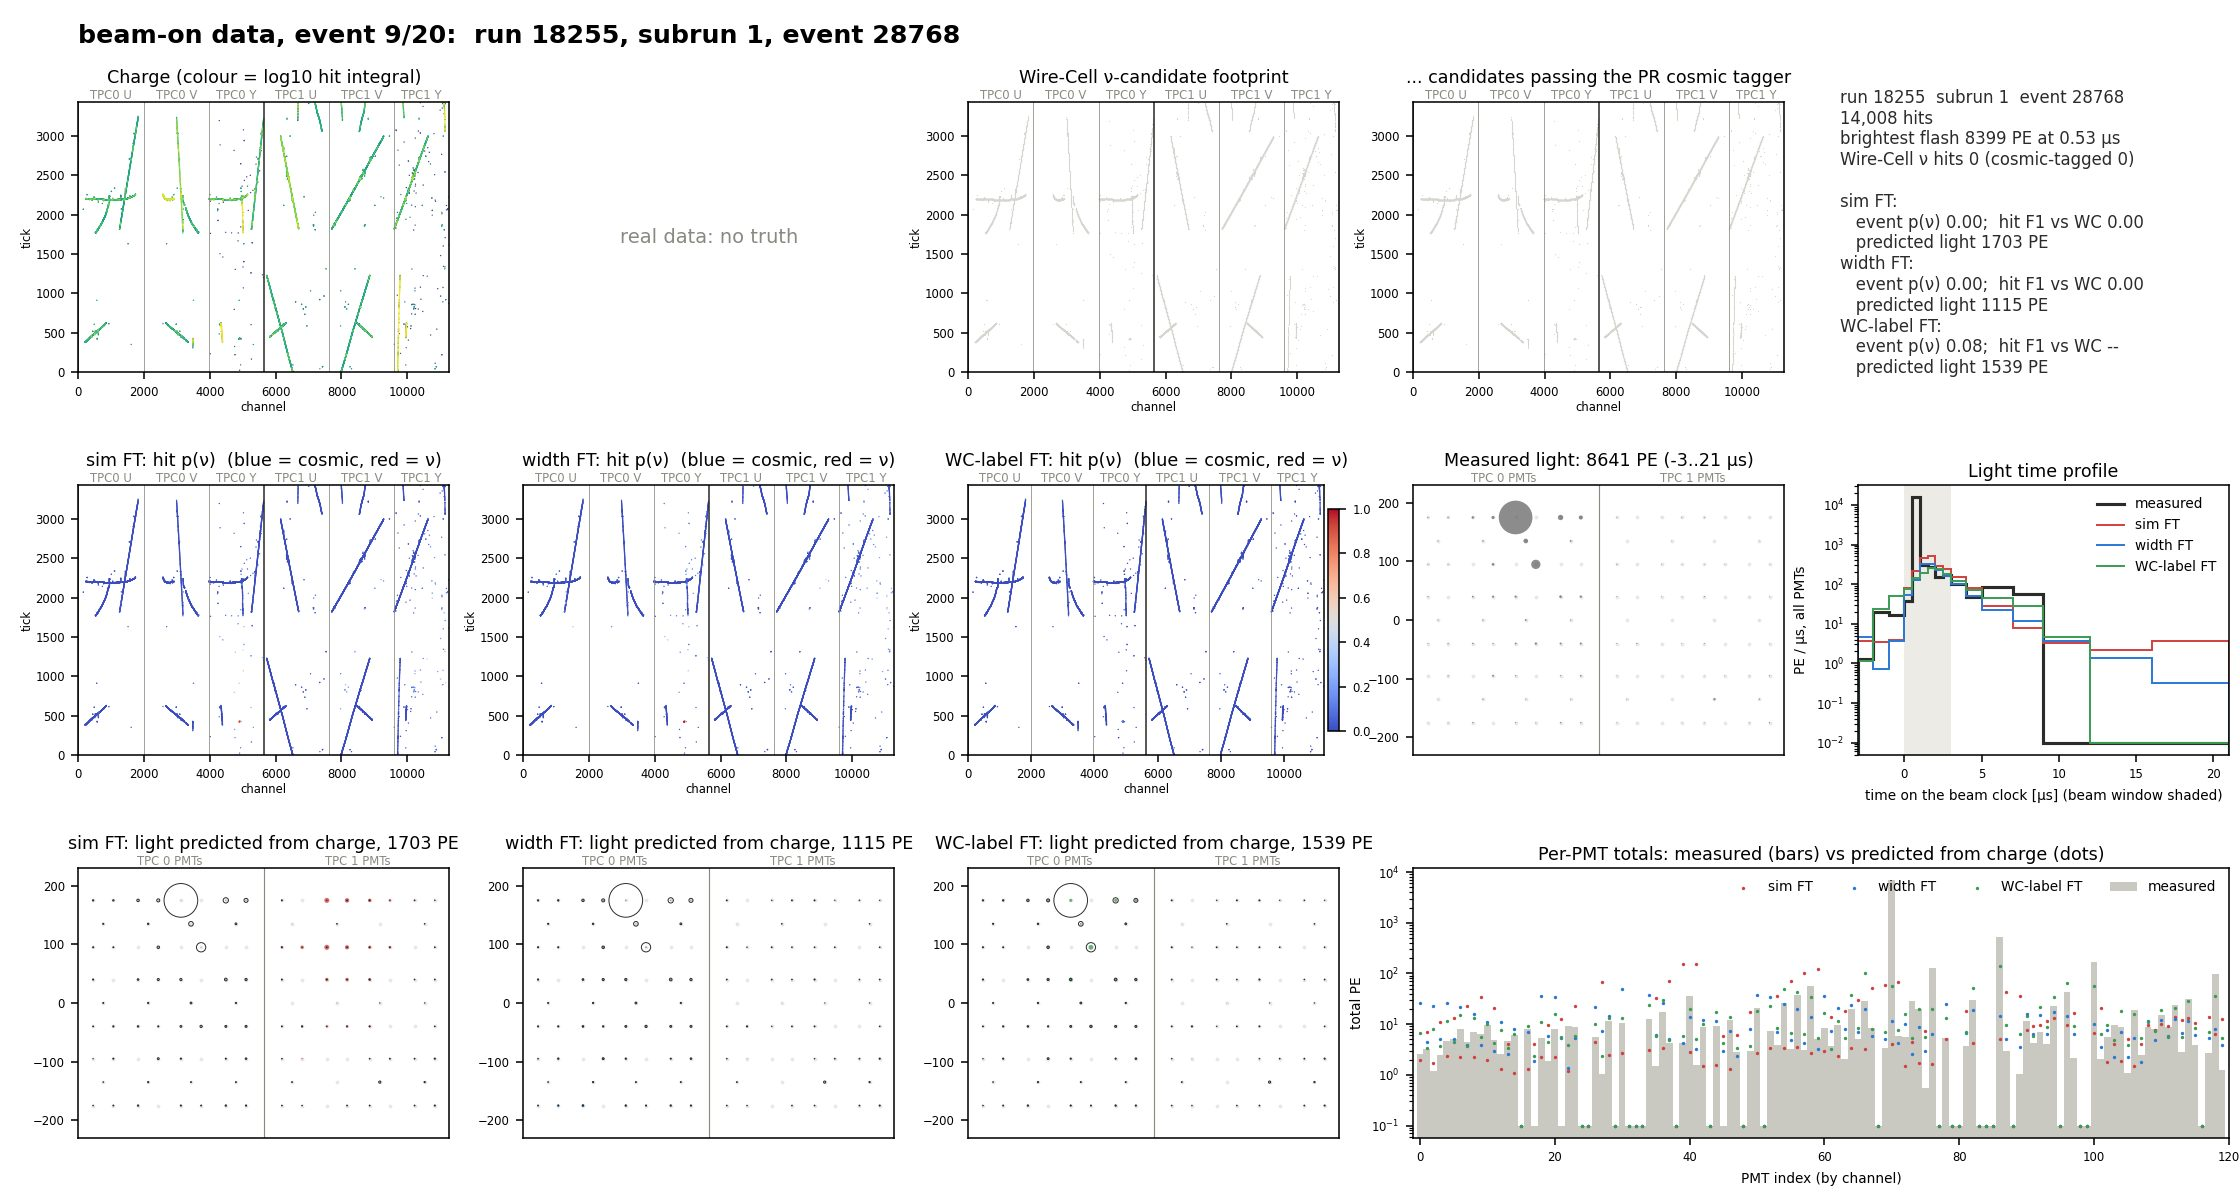
\includegraphics[width=\paperwidth,height=\paperheight,keepaspectratio]{displays/on_08.jpg}}
\end{frame}
% Beam-on data 10/20: run 18259, subrun 1, event 258582; event p(nu): sim FT 0.00, width FT 0.00, WC-label FT 0.34
\begin{frame}[plain]
  \centering\vspace*{-2pt}
  \makebox[\linewidth][c]{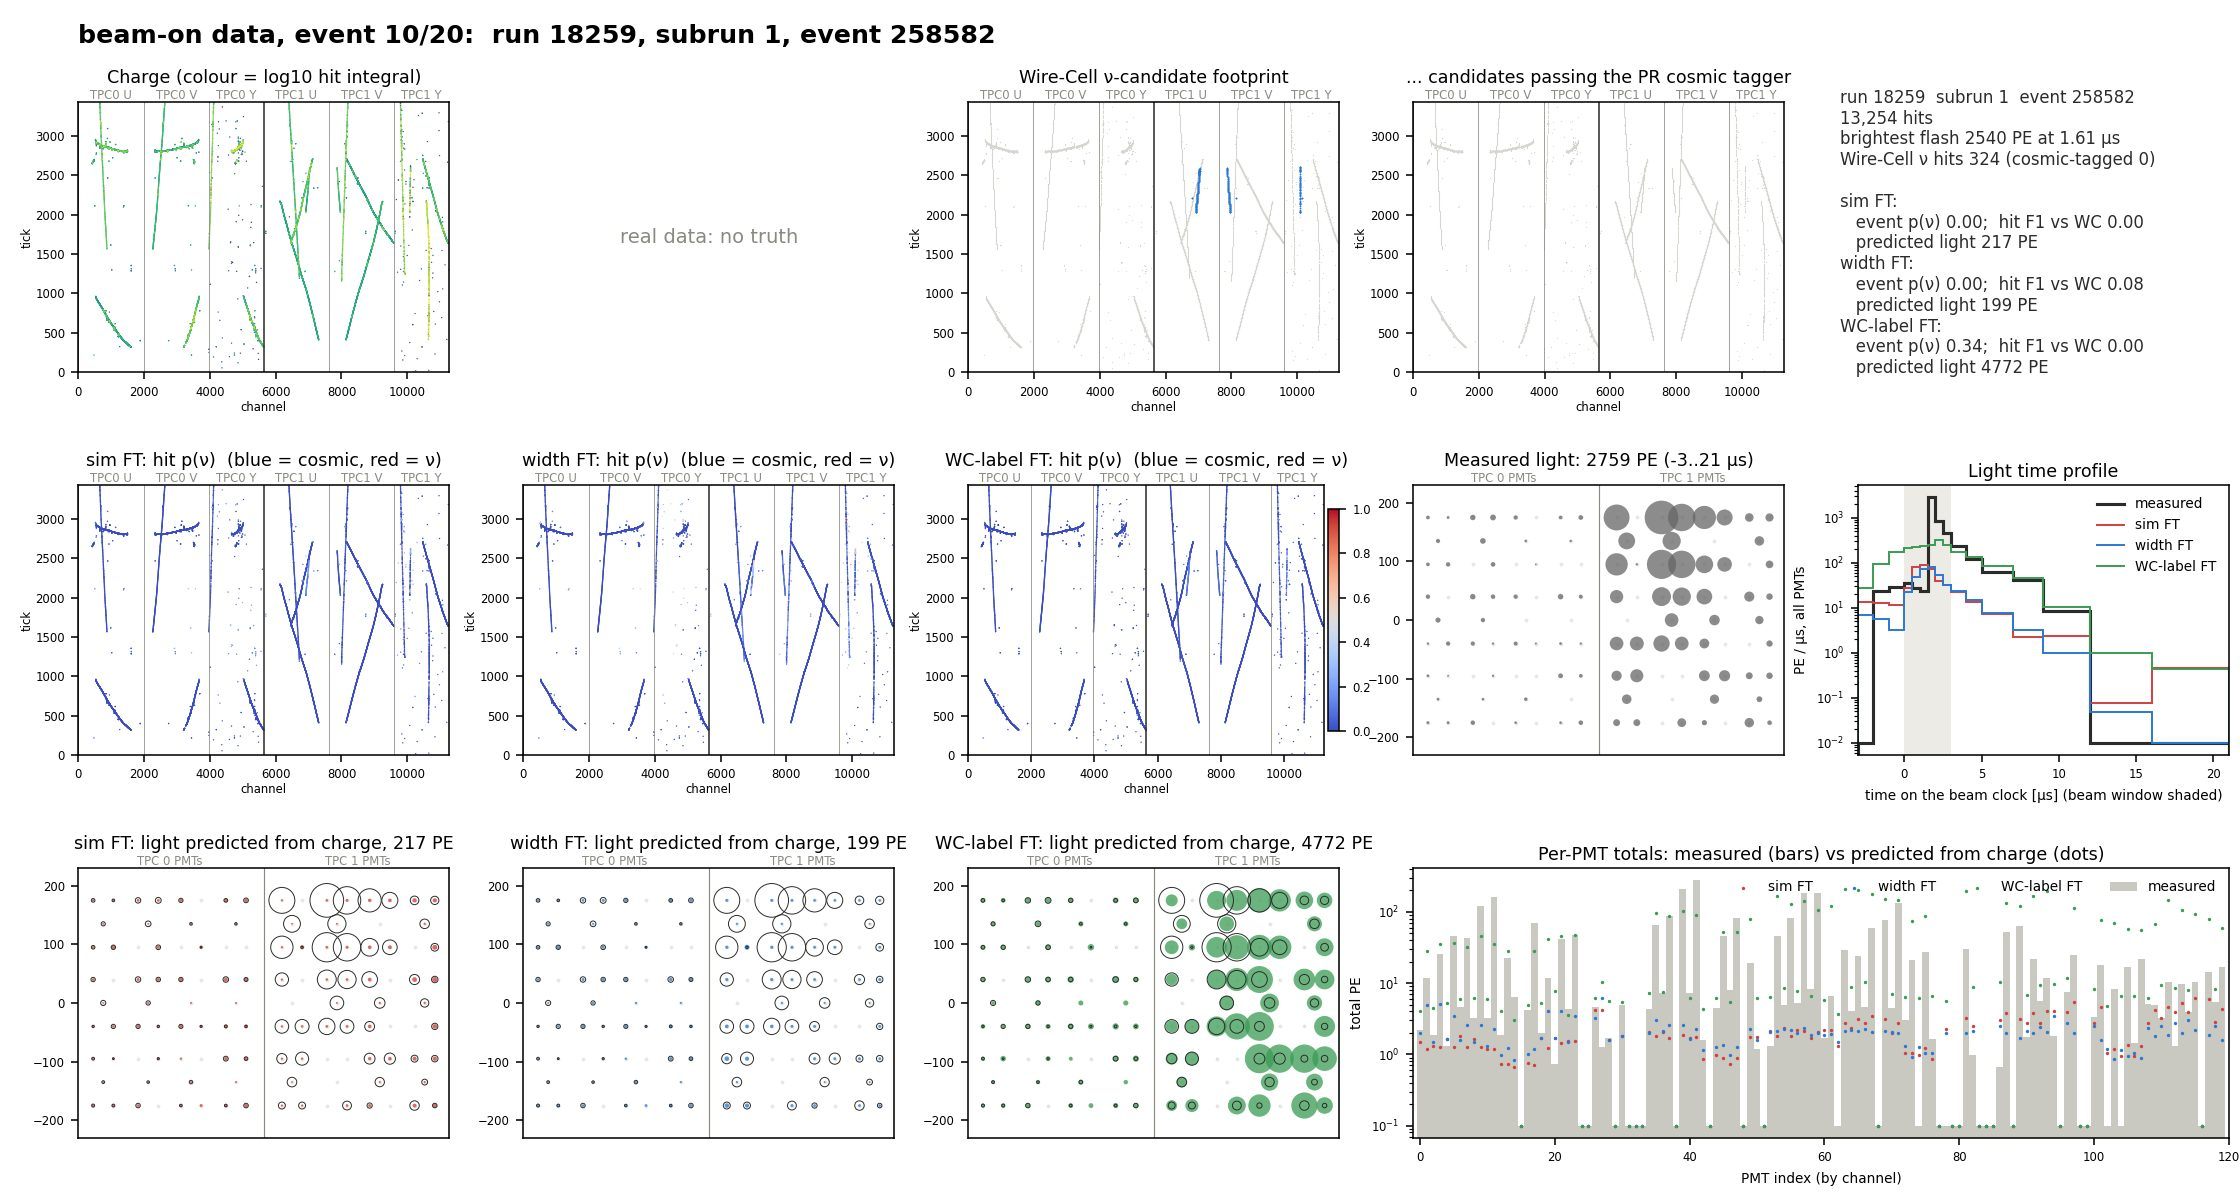
\includegraphics[width=\paperwidth,height=\paperheight,keepaspectratio]{displays/on_09.jpg}}
\end{frame}
% Beam-on data 11/20: run 18255, subrun 1, event 122922; event p(nu): sim FT 0.99, width FT 1.00, WC-label FT 0.17
\begin{frame}[plain]
  \centering\vspace*{-2pt}
  \makebox[\linewidth][c]{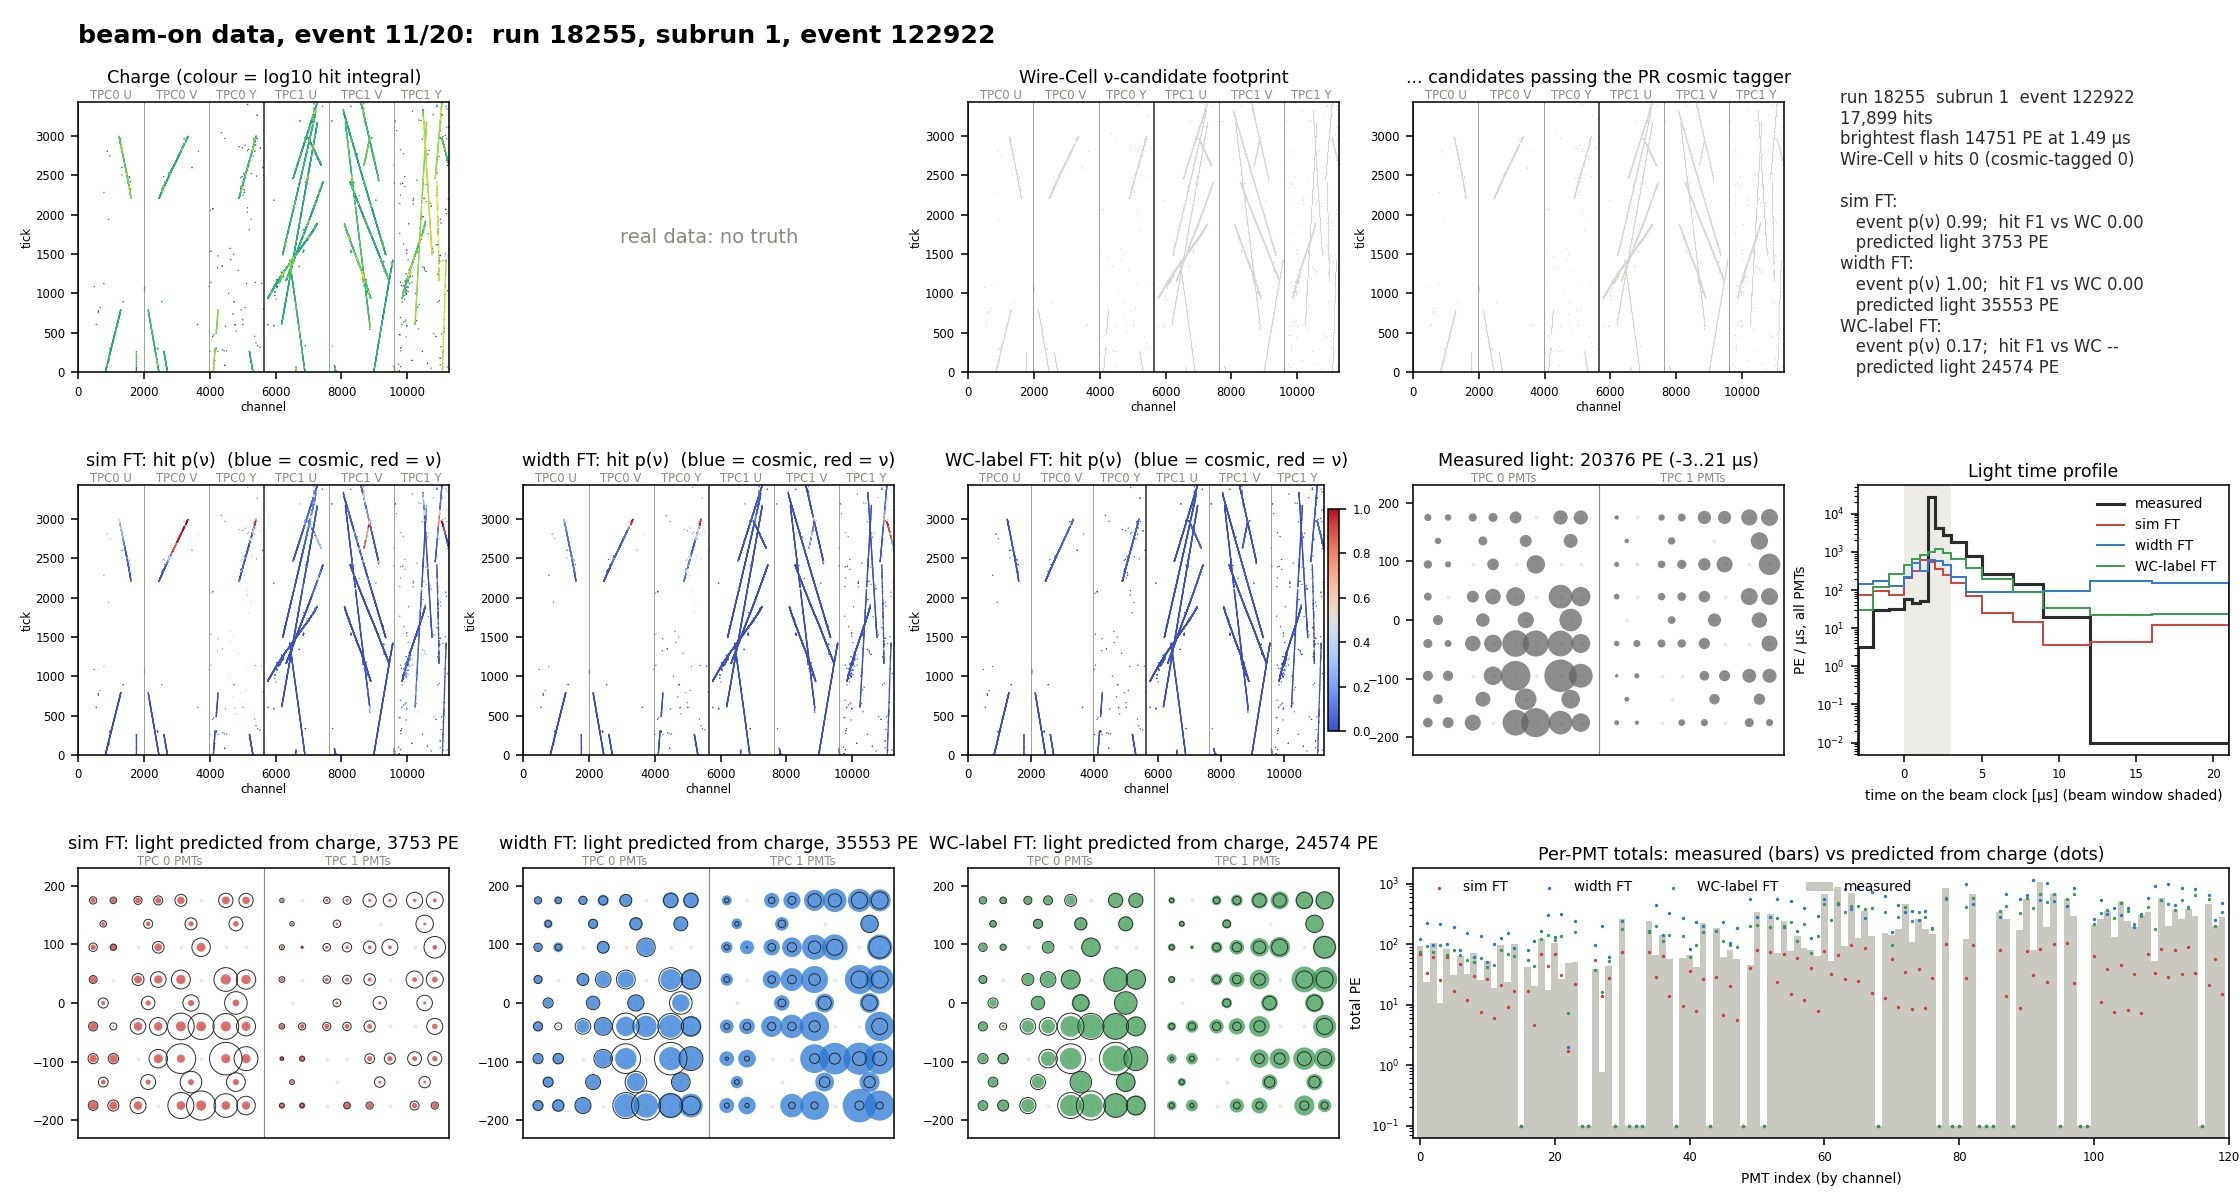
\includegraphics[width=\paperwidth,height=\paperheight,keepaspectratio]{displays/on_10.jpg}}
\end{frame}
% Beam-on data 12/20: run 18255, subrun 1, event 393542; event p(nu): sim FT 0.00, width FT 0.00, WC-label FT 0.49
\begin{frame}[plain]
  \centering\vspace*{-2pt}
  \makebox[\linewidth][c]{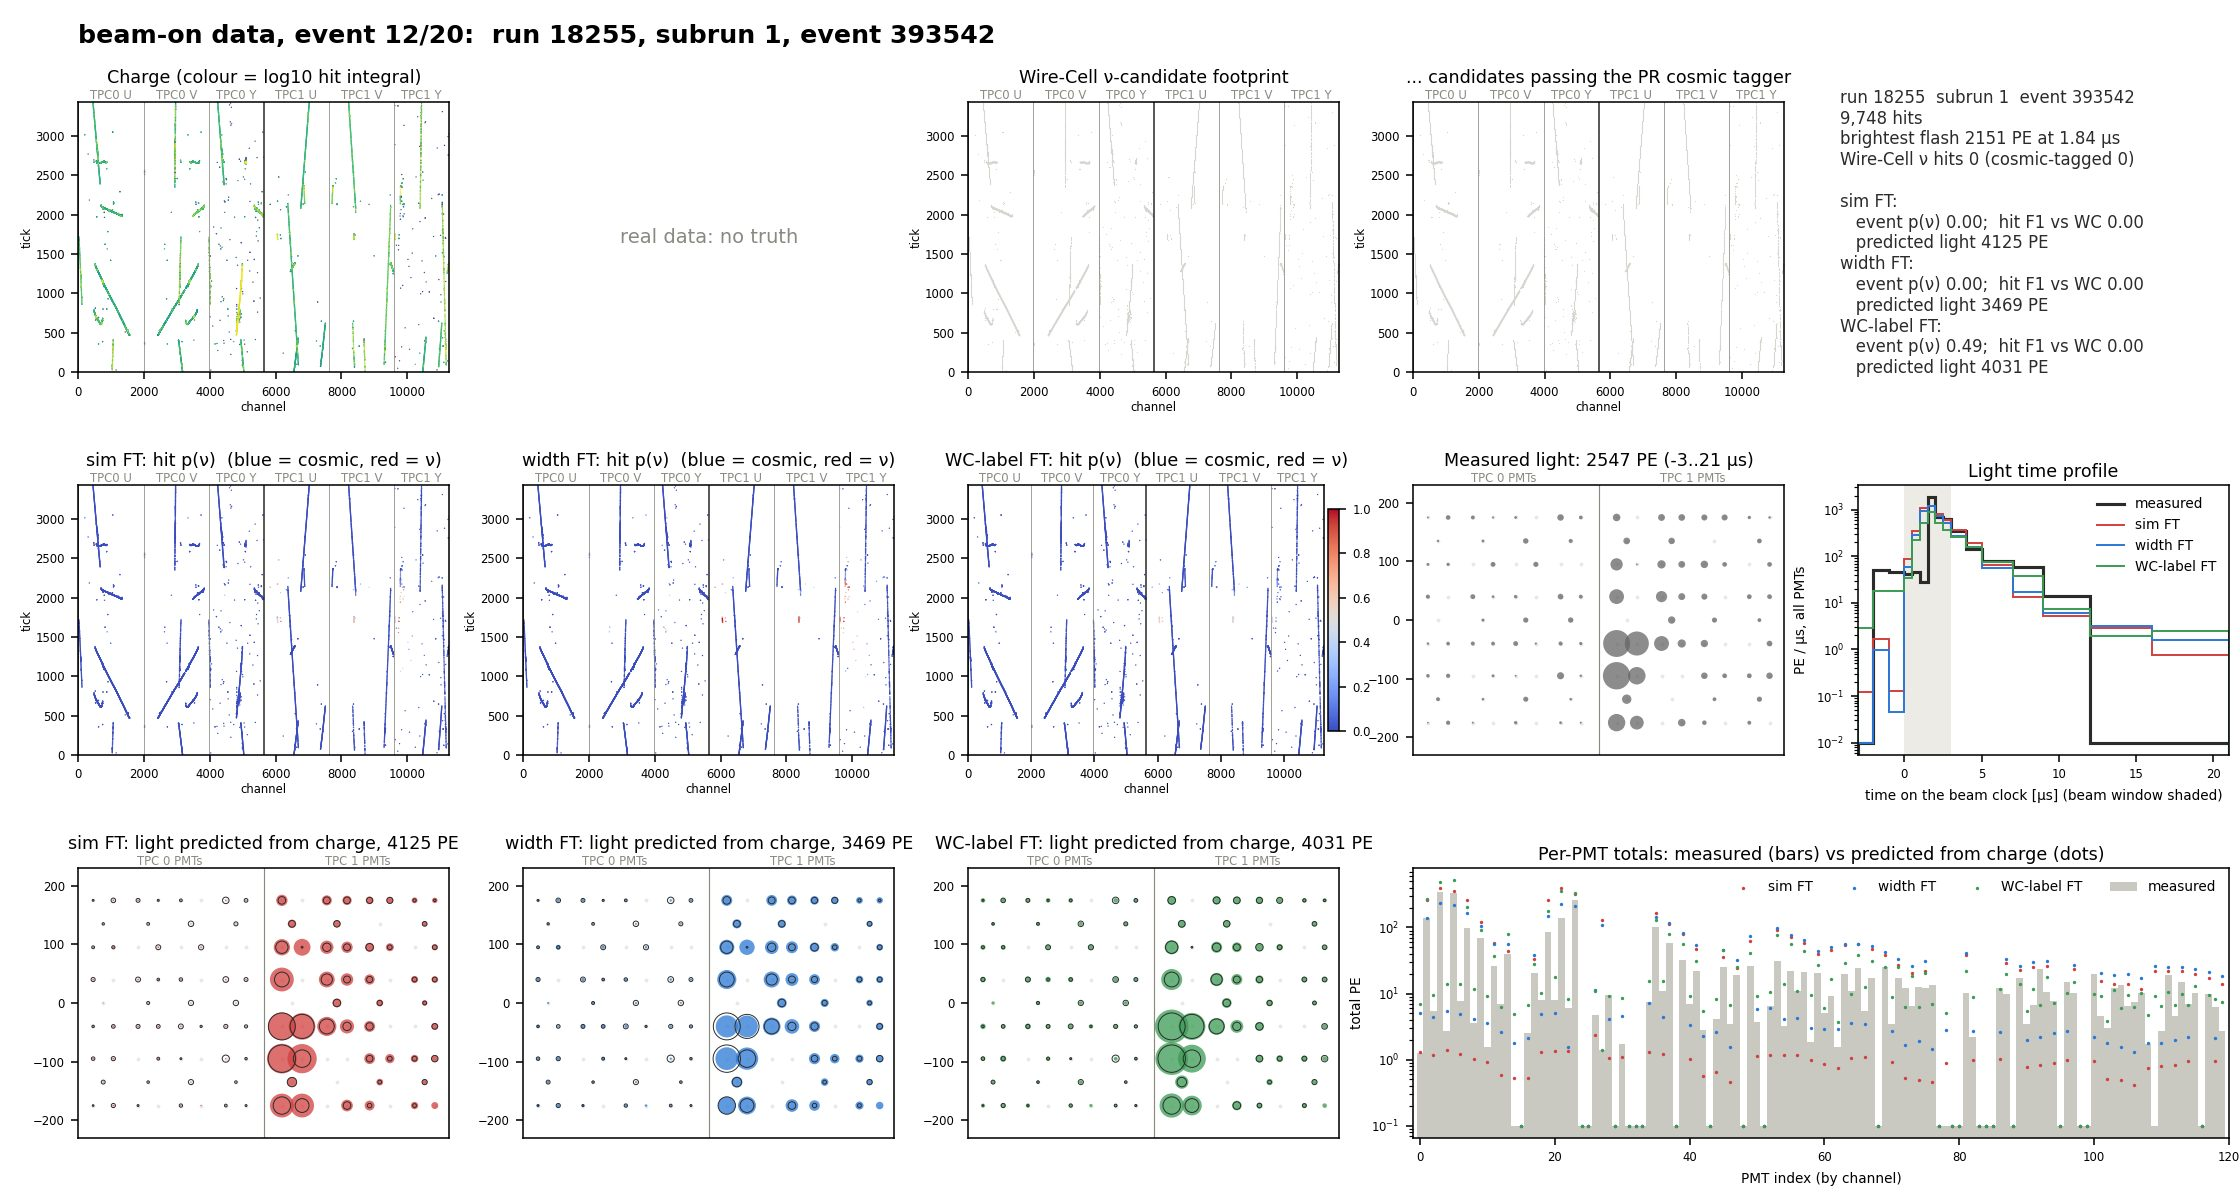
\includegraphics[width=\paperwidth,height=\paperheight,keepaspectratio]{displays/on_11.jpg}}
\end{frame}
% Beam-on data 13/20: run 18255, subrun 1, event 390700; event p(nu): sim FT 0.00, width FT 0.00, WC-label FT 0.11
\begin{frame}[plain]
  \centering\vspace*{-2pt}
  \makebox[\linewidth][c]{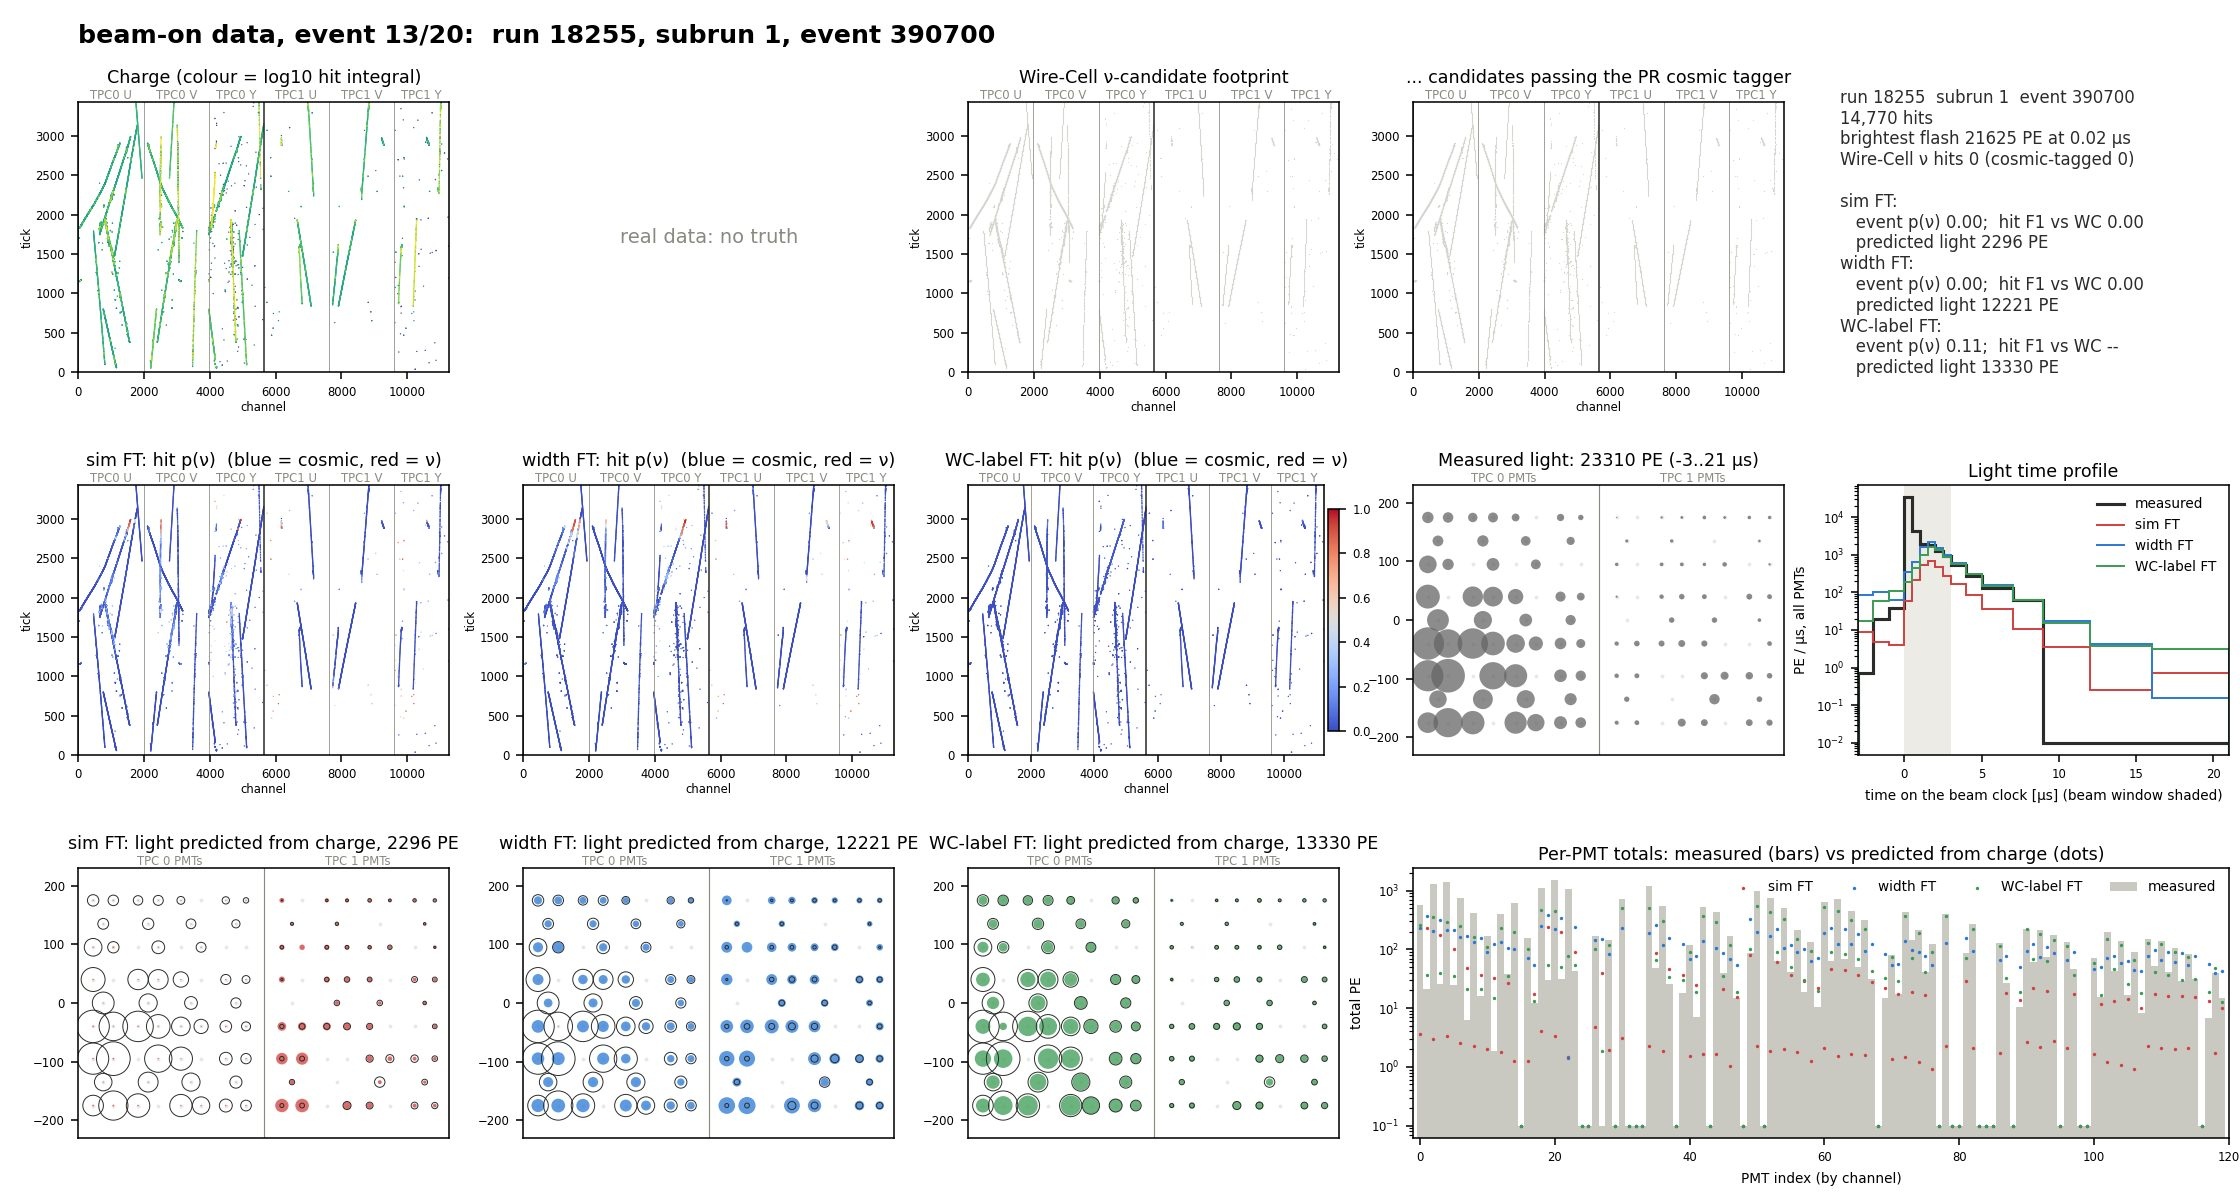
\includegraphics[width=\paperwidth,height=\paperheight,keepaspectratio]{displays/on_12.jpg}}
\end{frame}
% Beam-on data 14/20: run 18255, subrun 1, event 136435; event p(nu): sim FT 1.00, width FT 1.00, WC-label FT 0.99
\begin{frame}[plain]
  \centering\vspace*{-2pt}
  \makebox[\linewidth][c]{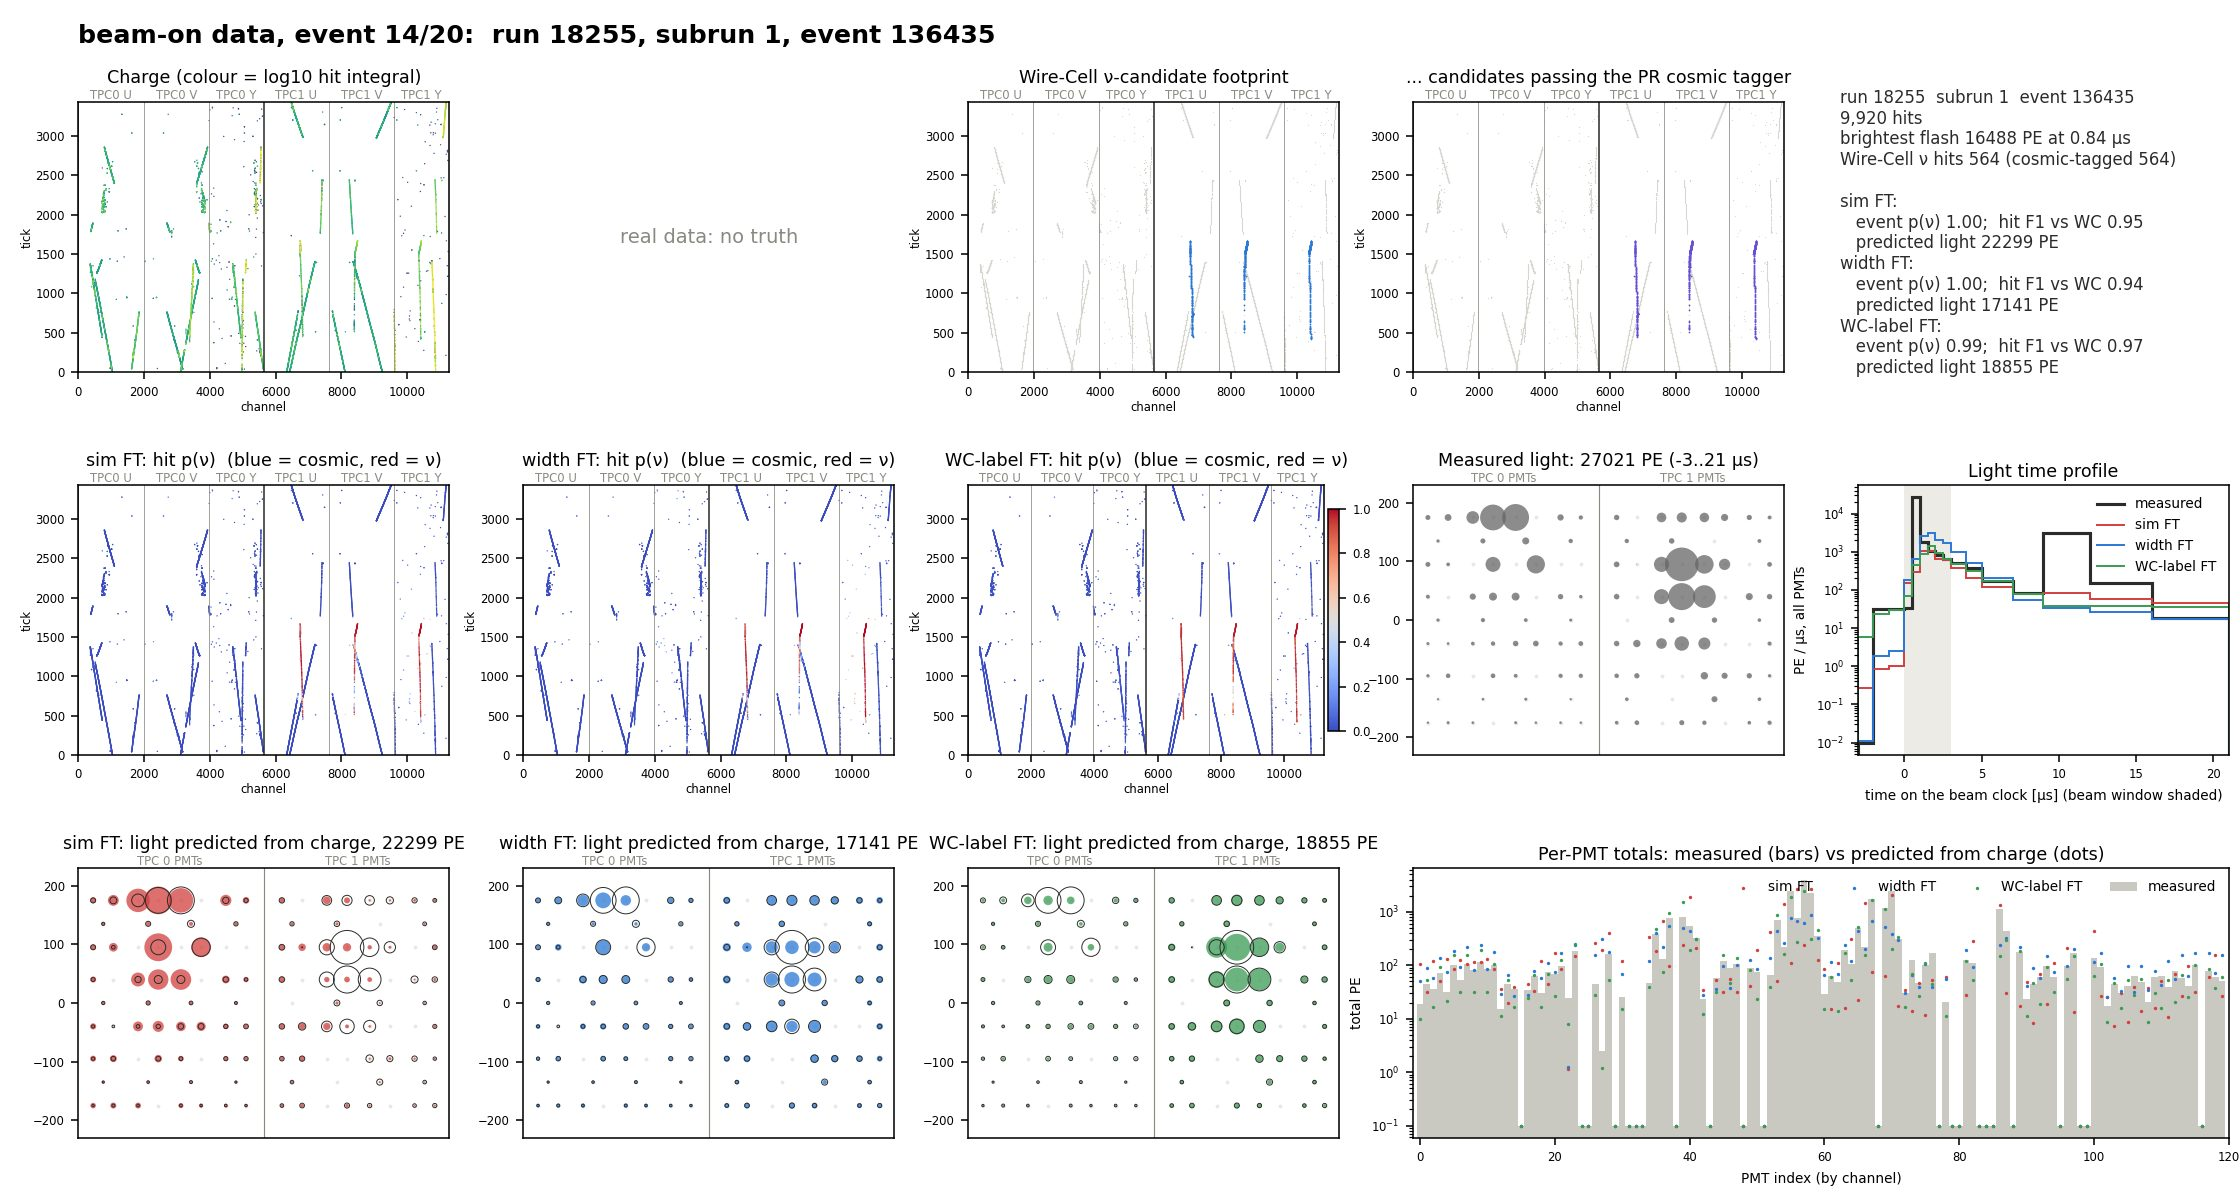
\includegraphics[width=\paperwidth,height=\paperheight,keepaspectratio]{displays/on_13.jpg}}
\end{frame}
% Beam-on data 15/20: run 18255, subrun 1, event 339420; event p(nu): sim FT 0.13, width FT 0.00, WC-label FT 0.80
\begin{frame}[plain]
  \centering\vspace*{-2pt}
  \makebox[\linewidth][c]{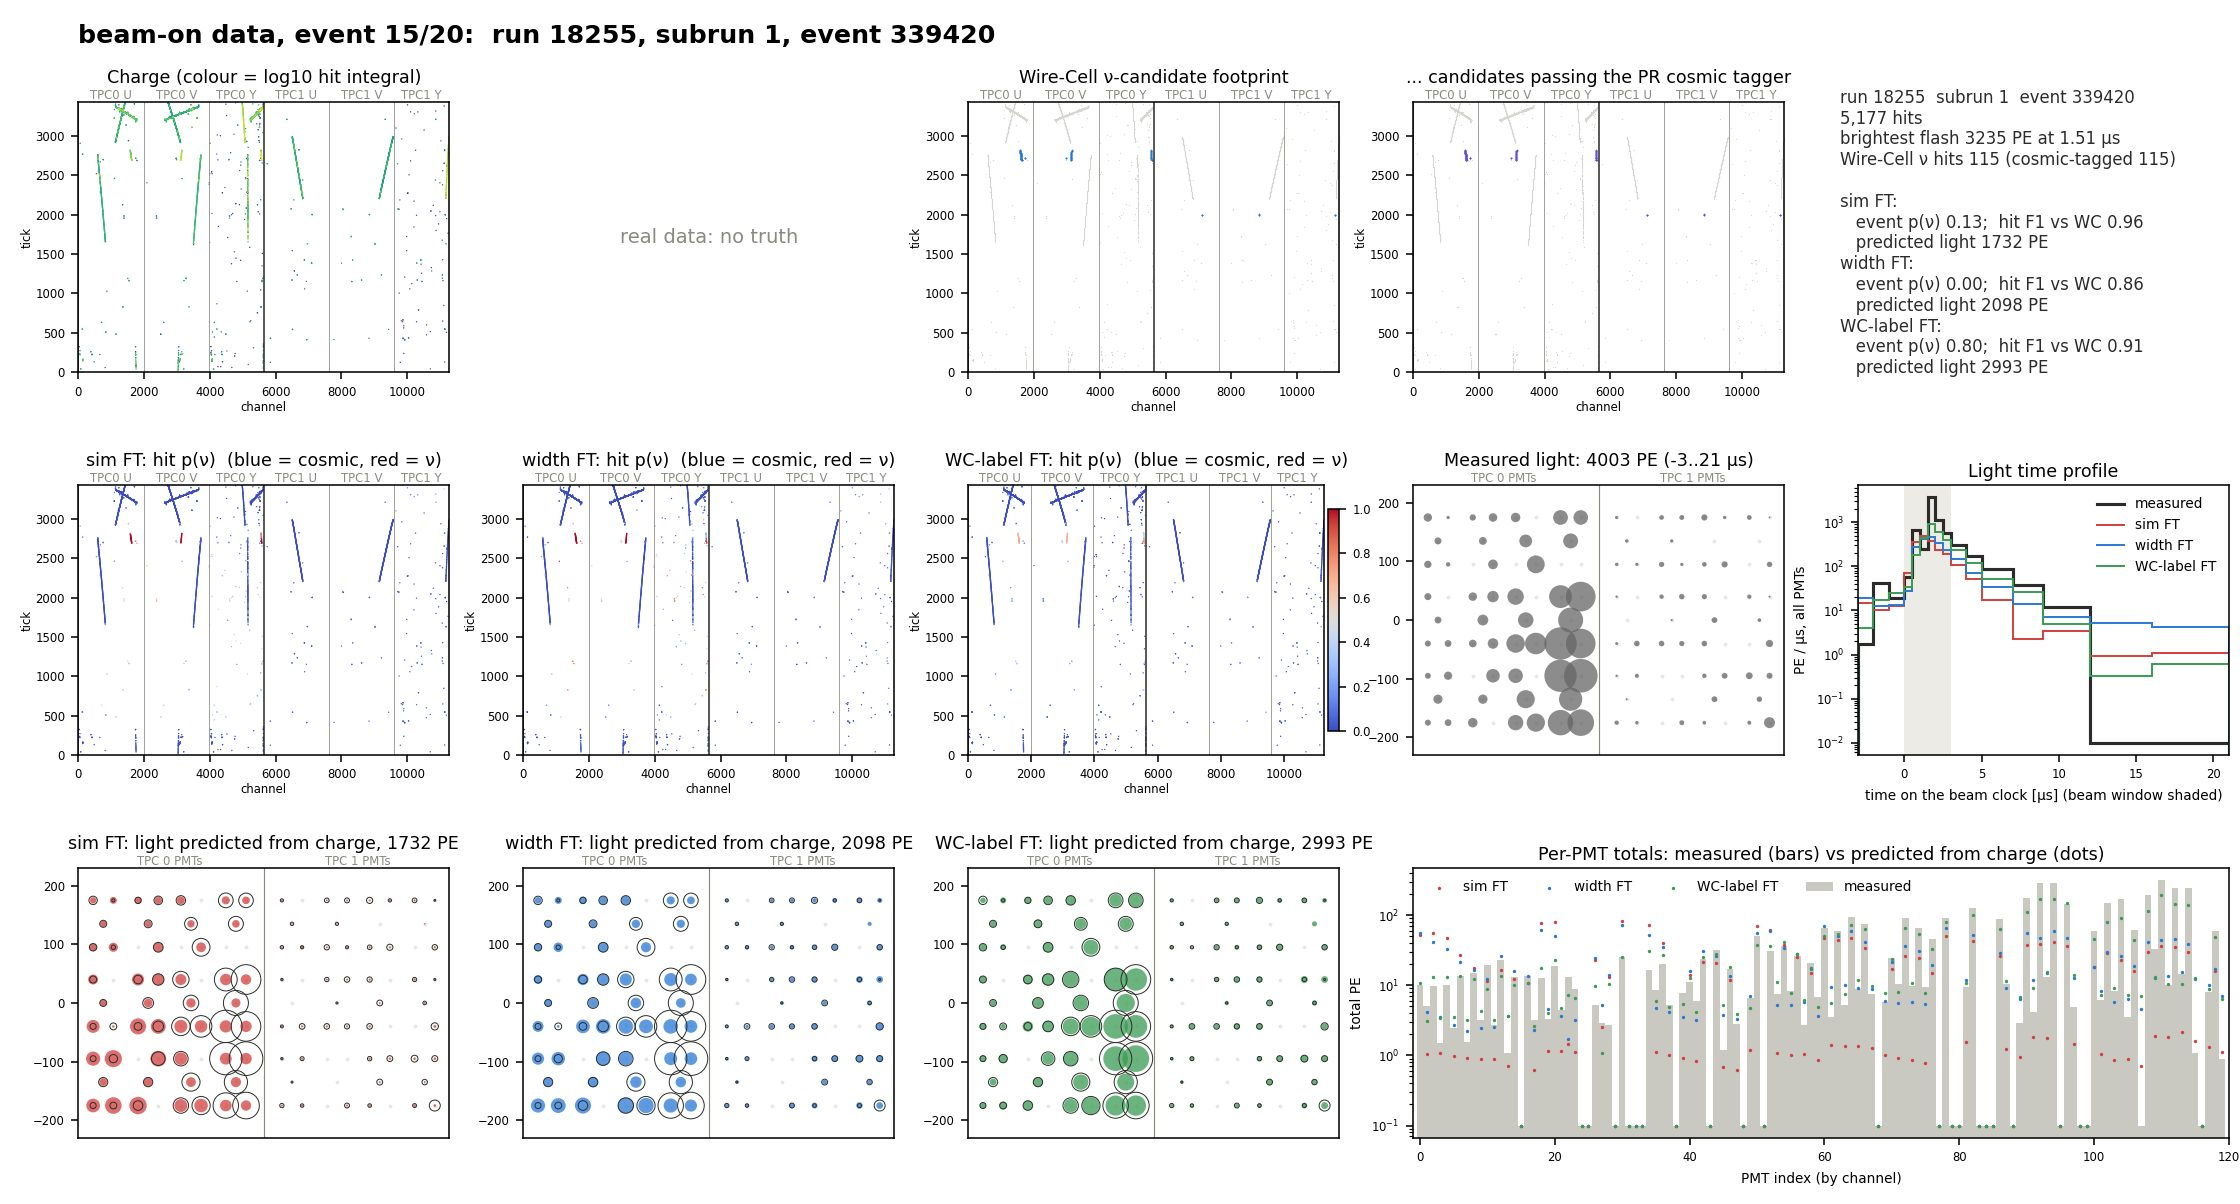
\includegraphics[width=\paperwidth,height=\paperheight,keepaspectratio]{displays/on_14.jpg}}
\end{frame}
% Beam-on data 16/20: run 18259, subrun 1, event 236590; event p(nu): sim FT 1.00, width FT 0.61, WC-label FT 0.72
\begin{frame}[plain]
  \centering\vspace*{-2pt}
  \makebox[\linewidth][c]{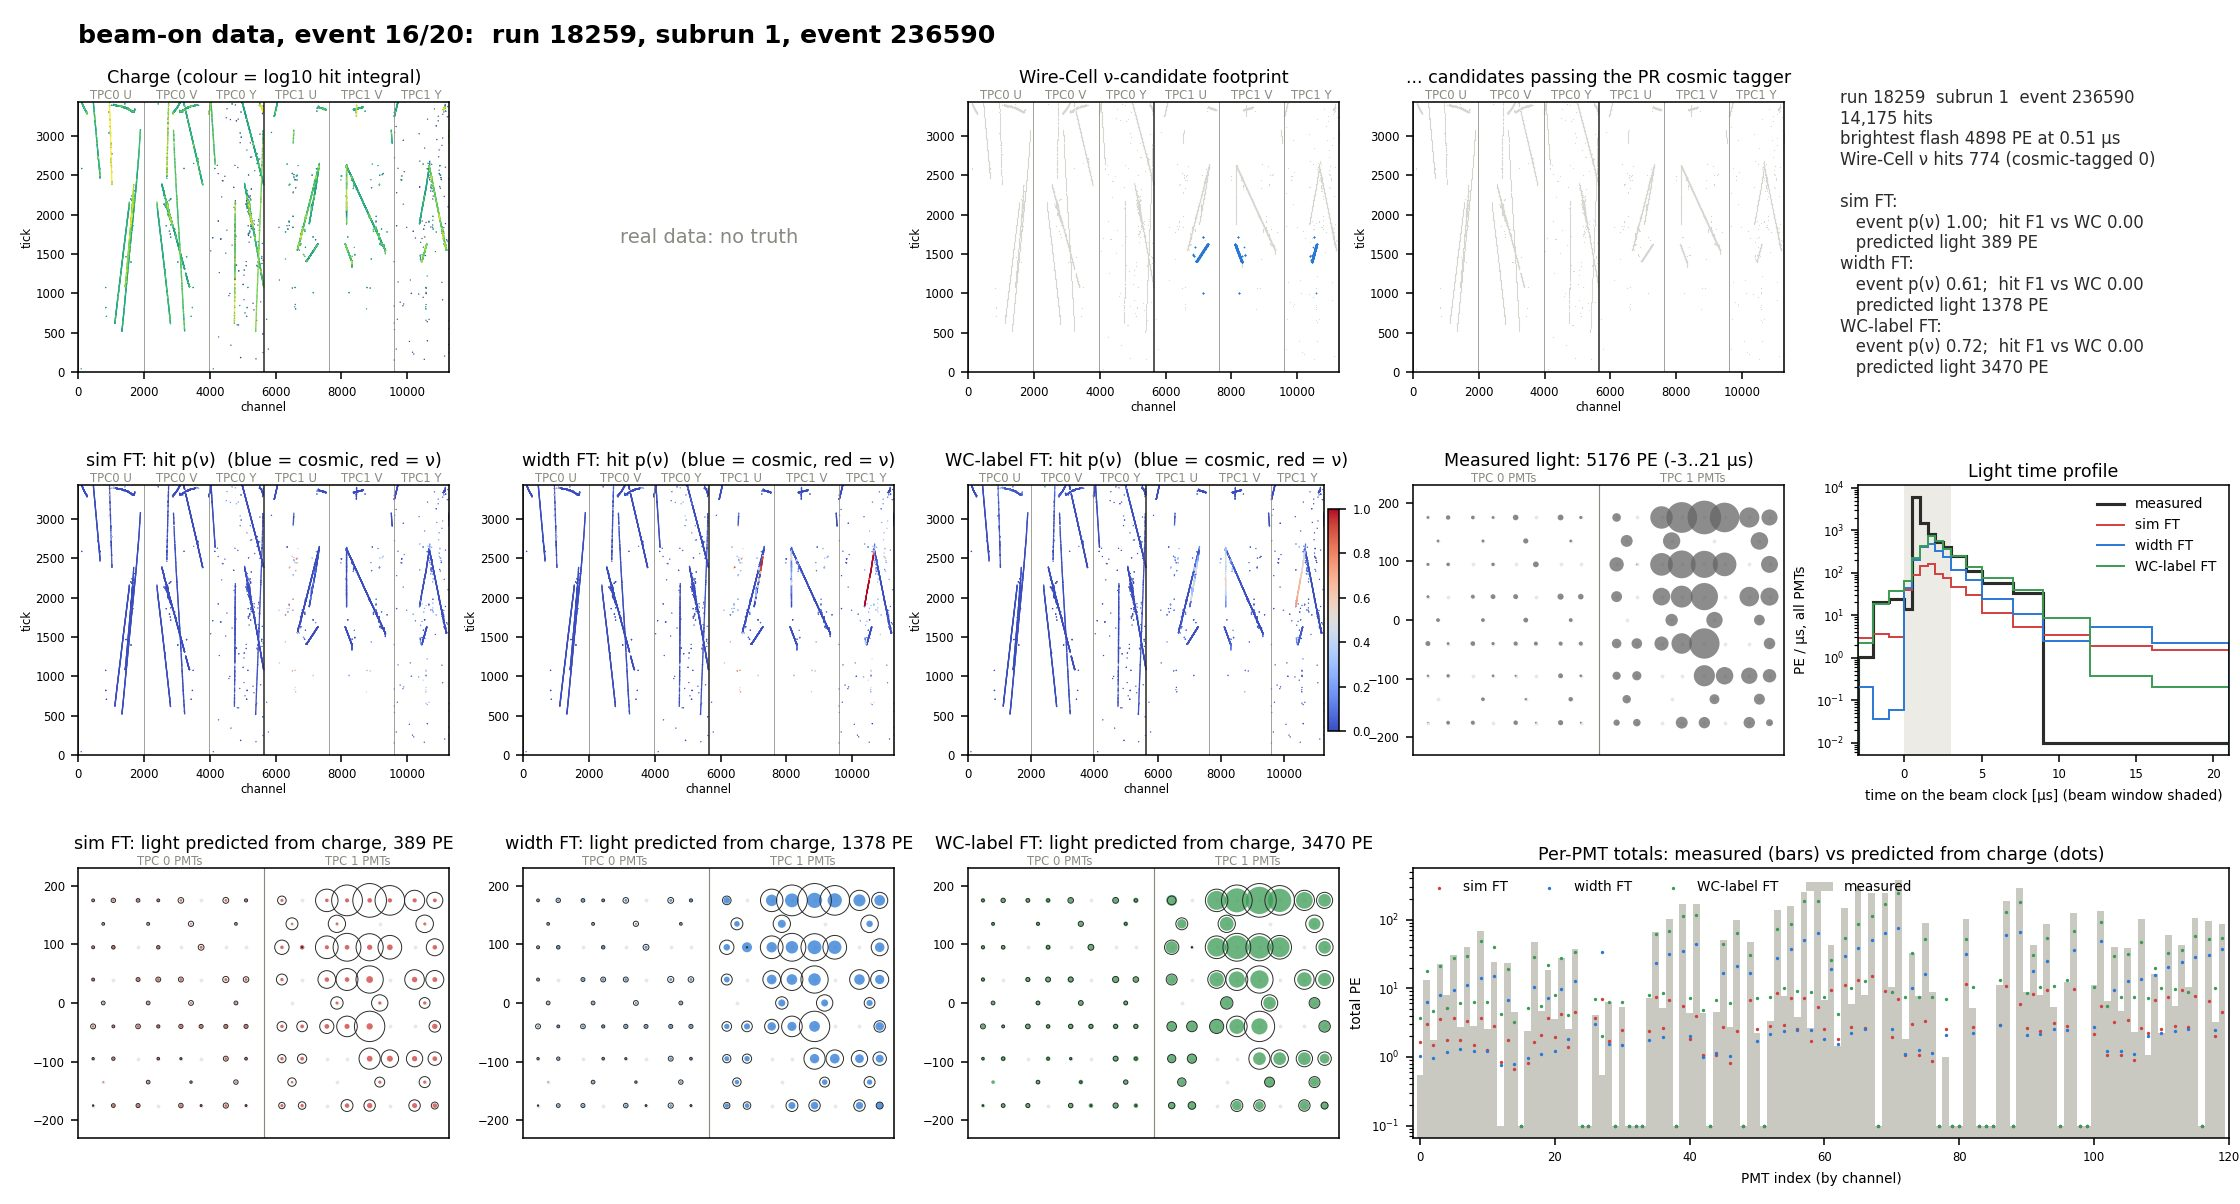
\includegraphics[width=\paperwidth,height=\paperheight,keepaspectratio]{displays/on_15.jpg}}
\end{frame}
% Beam-on data 17/20: run 18255, subrun 1, event 157835; event p(nu): sim FT 0.00, width FT 0.00, WC-label FT 0.62
\begin{frame}[plain]
  \centering\vspace*{-2pt}
  \makebox[\linewidth][c]{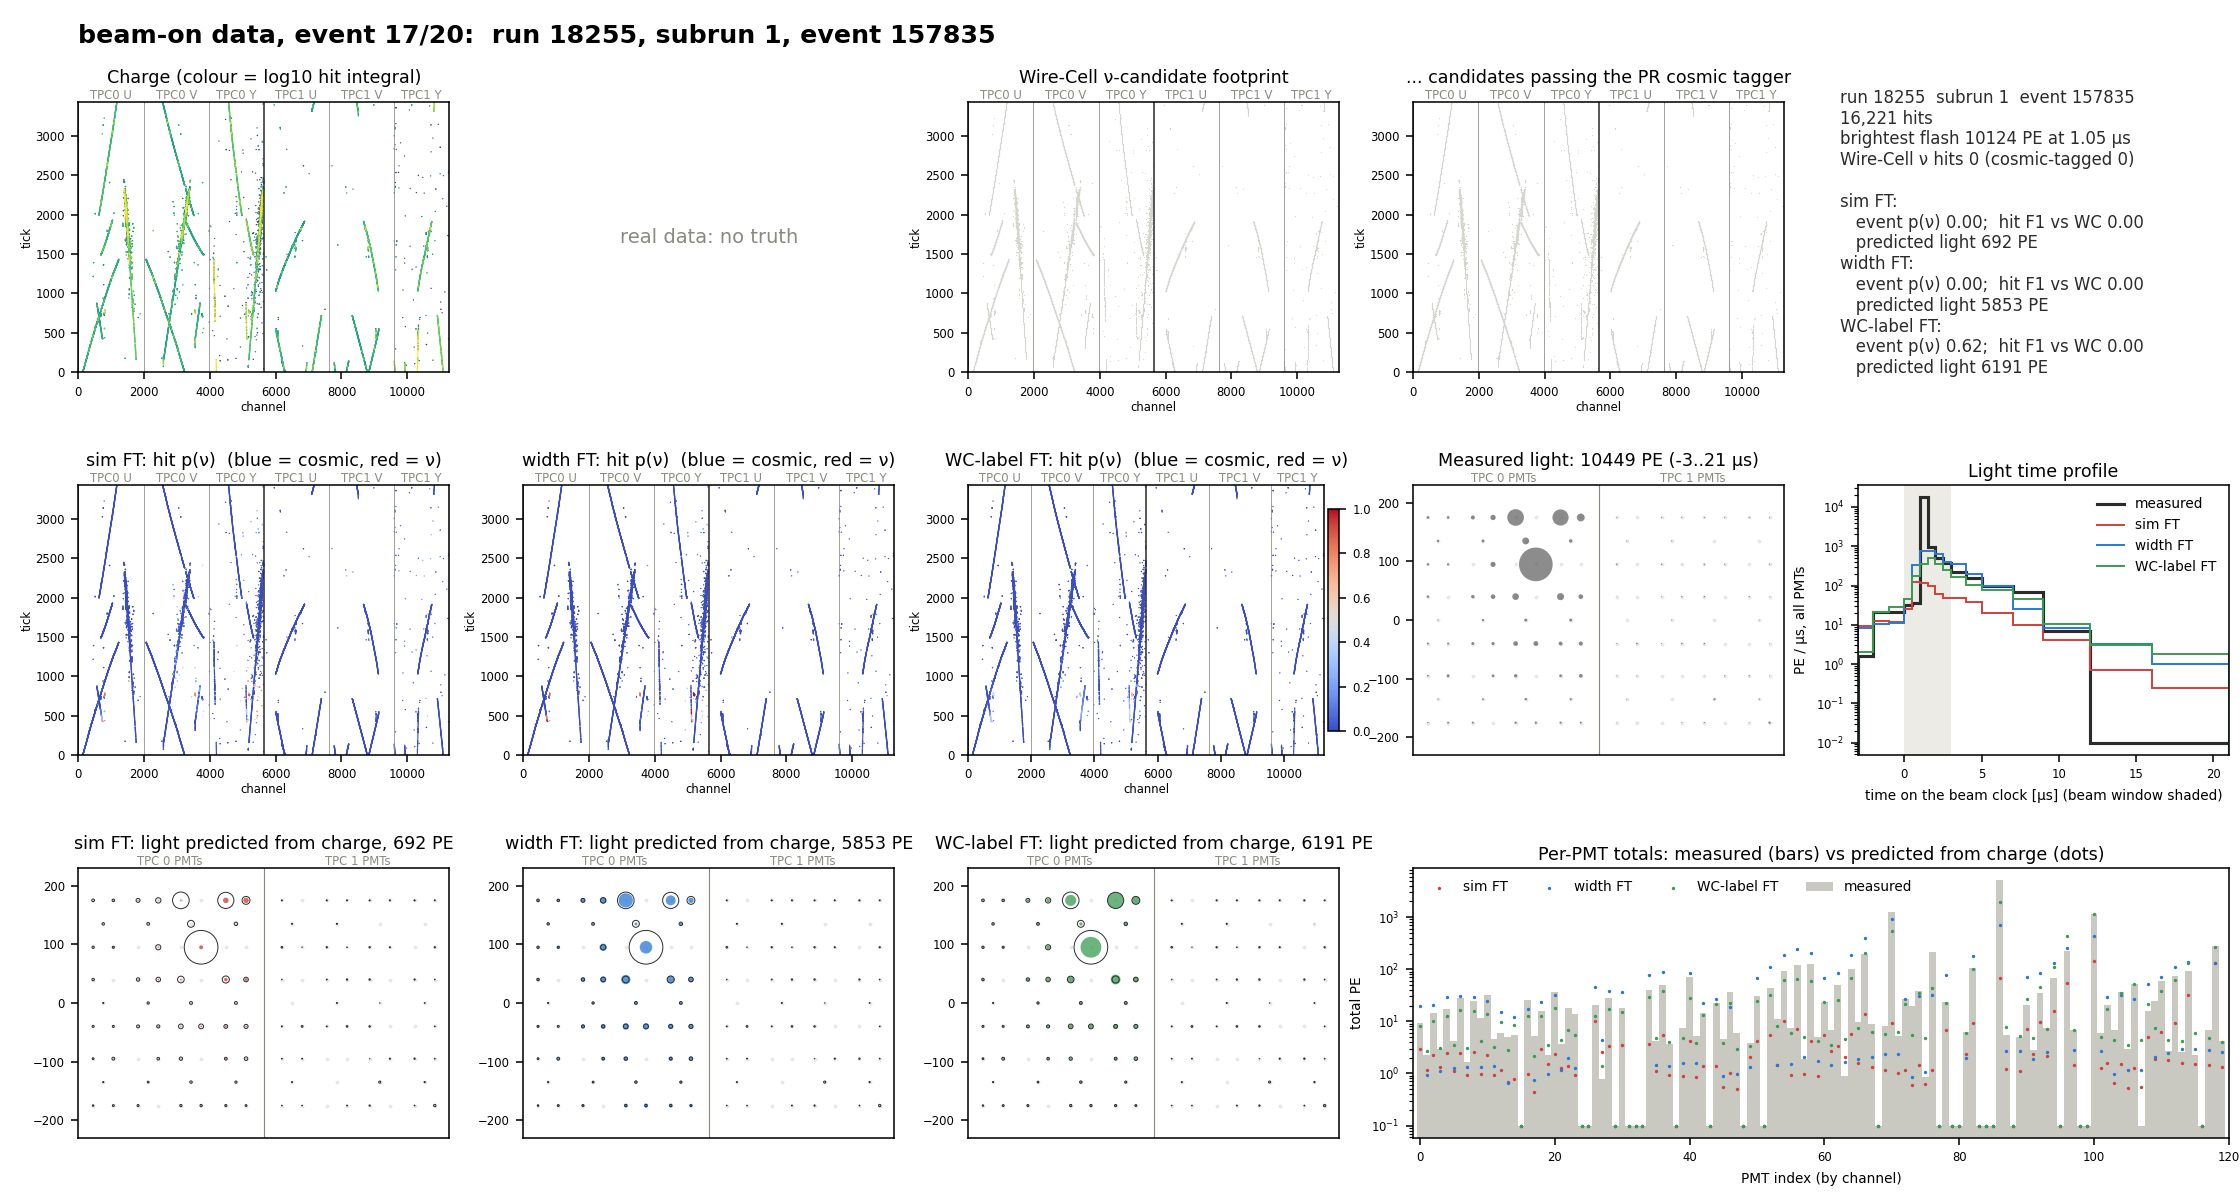
\includegraphics[width=\paperwidth,height=\paperheight,keepaspectratio]{displays/on_16.jpg}}
\end{frame}
% Beam-on data 18/20: run 18255, subrun 1, event 315441; event p(nu): sim FT 1.00, width FT 1.00, WC-label FT 0.88
\begin{frame}[plain]
  \centering\vspace*{-2pt}
  \makebox[\linewidth][c]{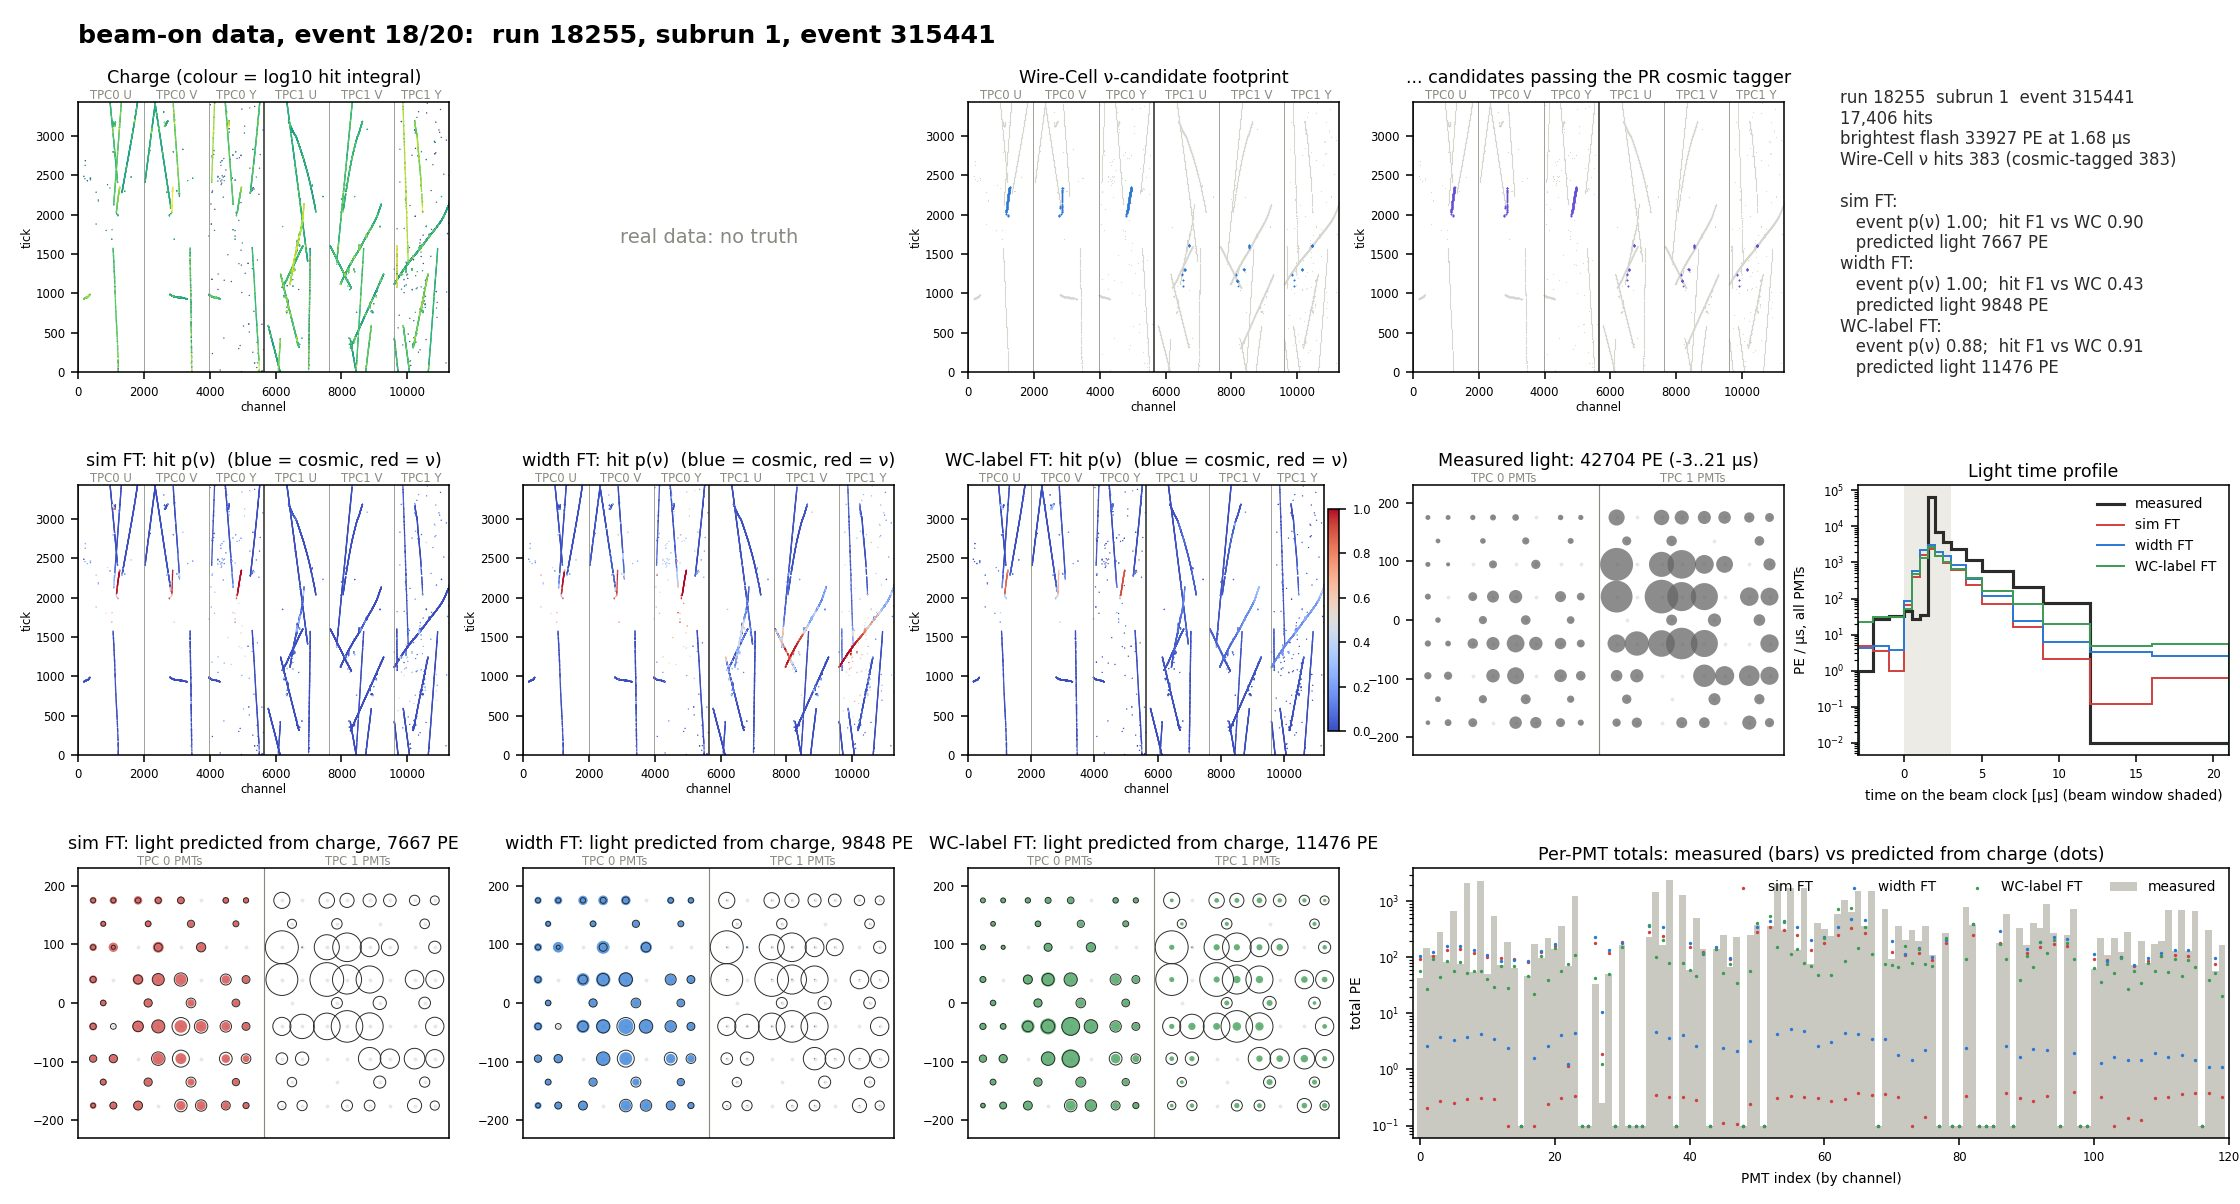
\includegraphics[width=\paperwidth,height=\paperheight,keepaspectratio]{displays/on_17.jpg}}
\end{frame}
% Beam-on data 19/20: run 18259, subrun 1, event 138755; event p(nu): sim FT 1.00, width FT 1.00, WC-label FT 0.98
\begin{frame}[plain]
  \centering\vspace*{-2pt}
  \makebox[\linewidth][c]{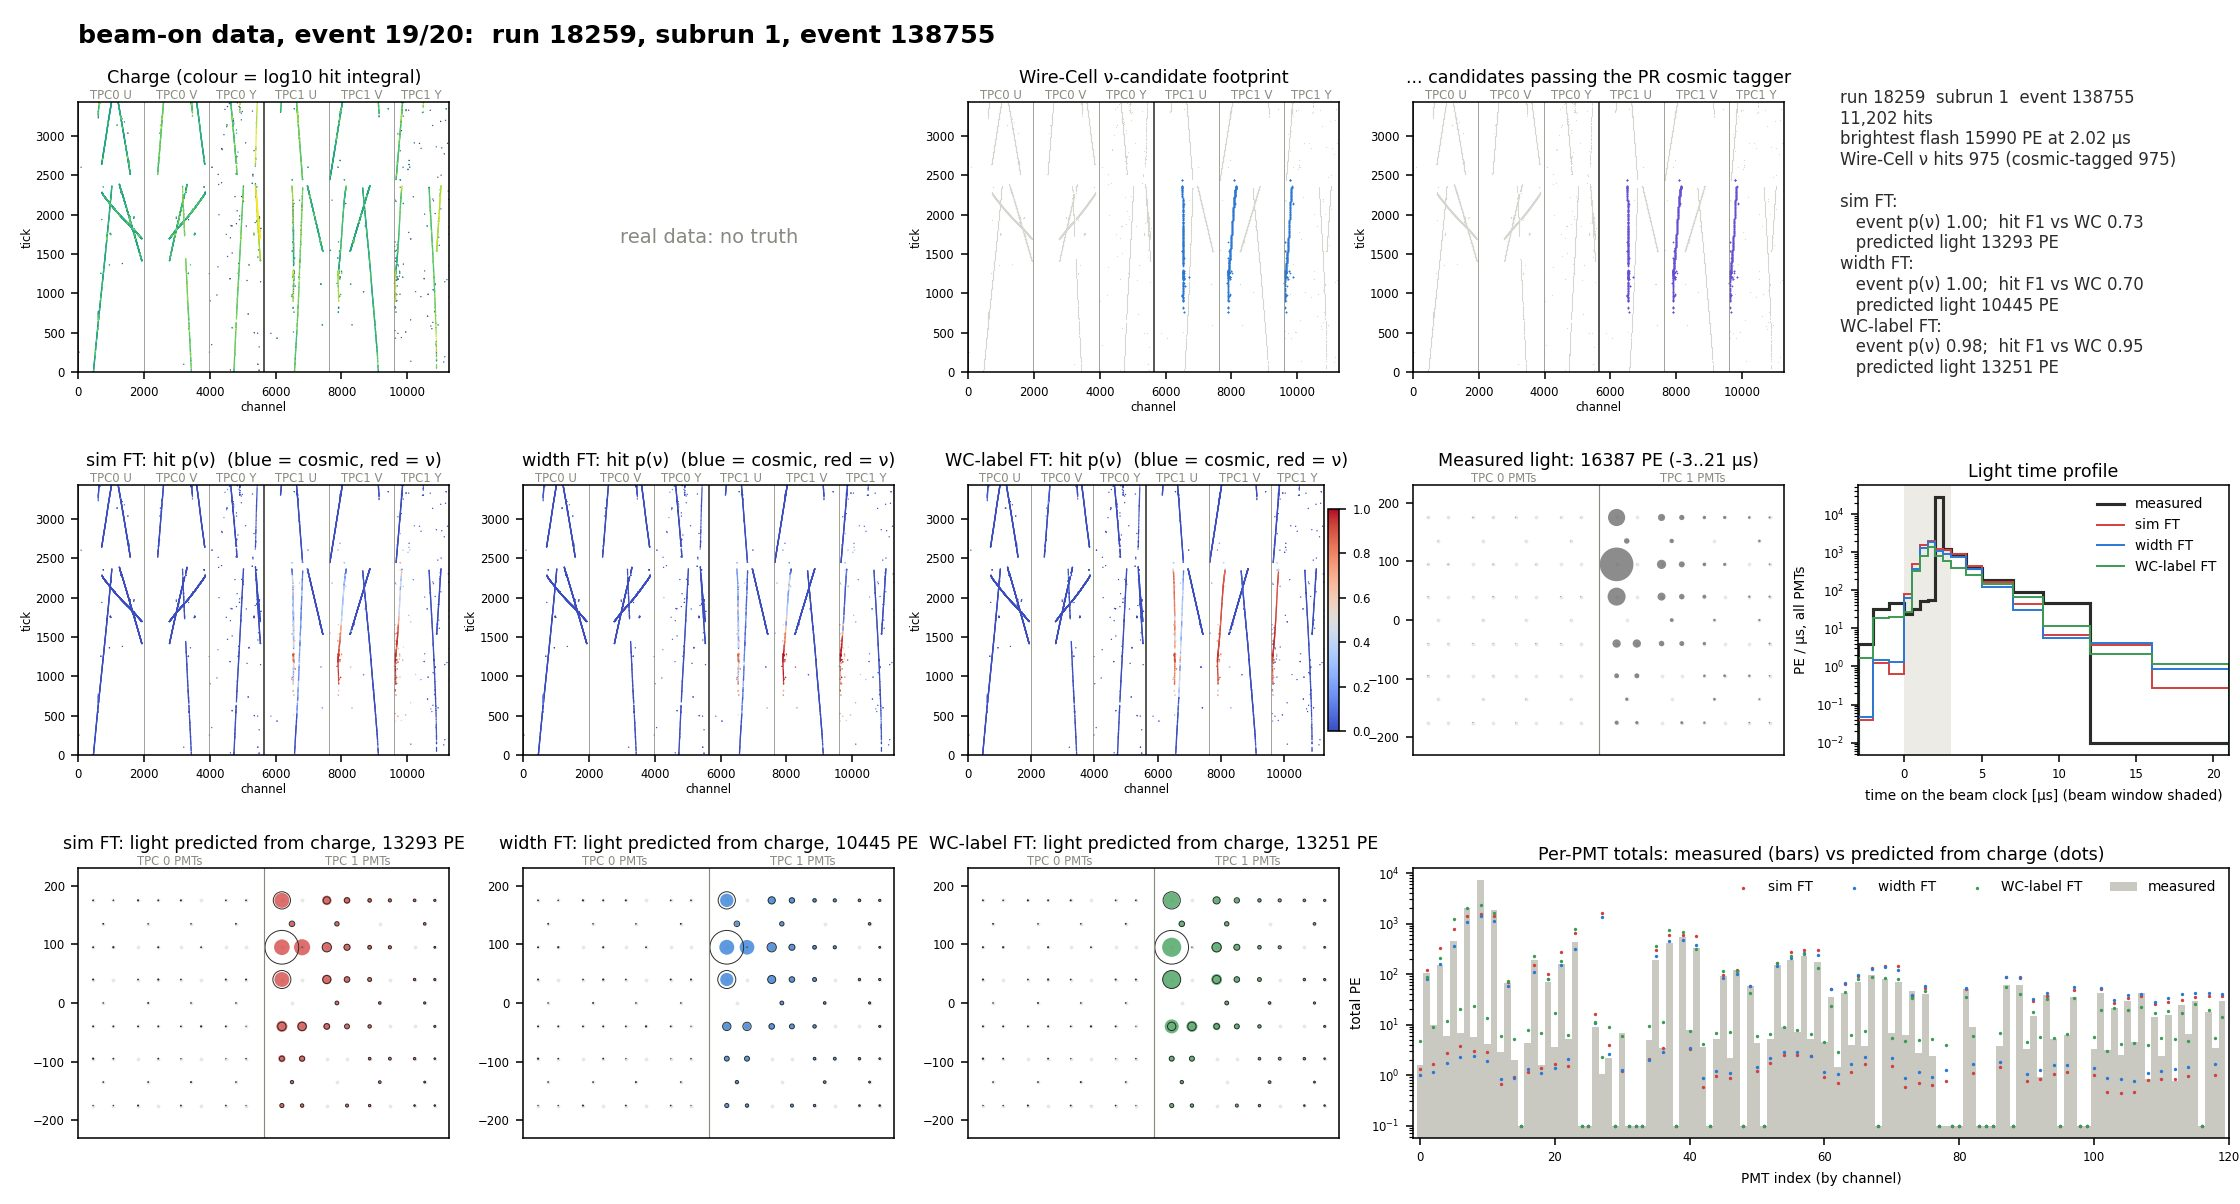
\includegraphics[width=\paperwidth,height=\paperheight,keepaspectratio]{displays/on_18.jpg}}
\end{frame}
% Beam-on data 20/20: run 18255, subrun 1, event 24654; event p(nu): sim FT 1.00, width FT 1.00, WC-label FT 0.97
\begin{frame}[plain]
  \centering\vspace*{-2pt}
  \makebox[\linewidth][c]{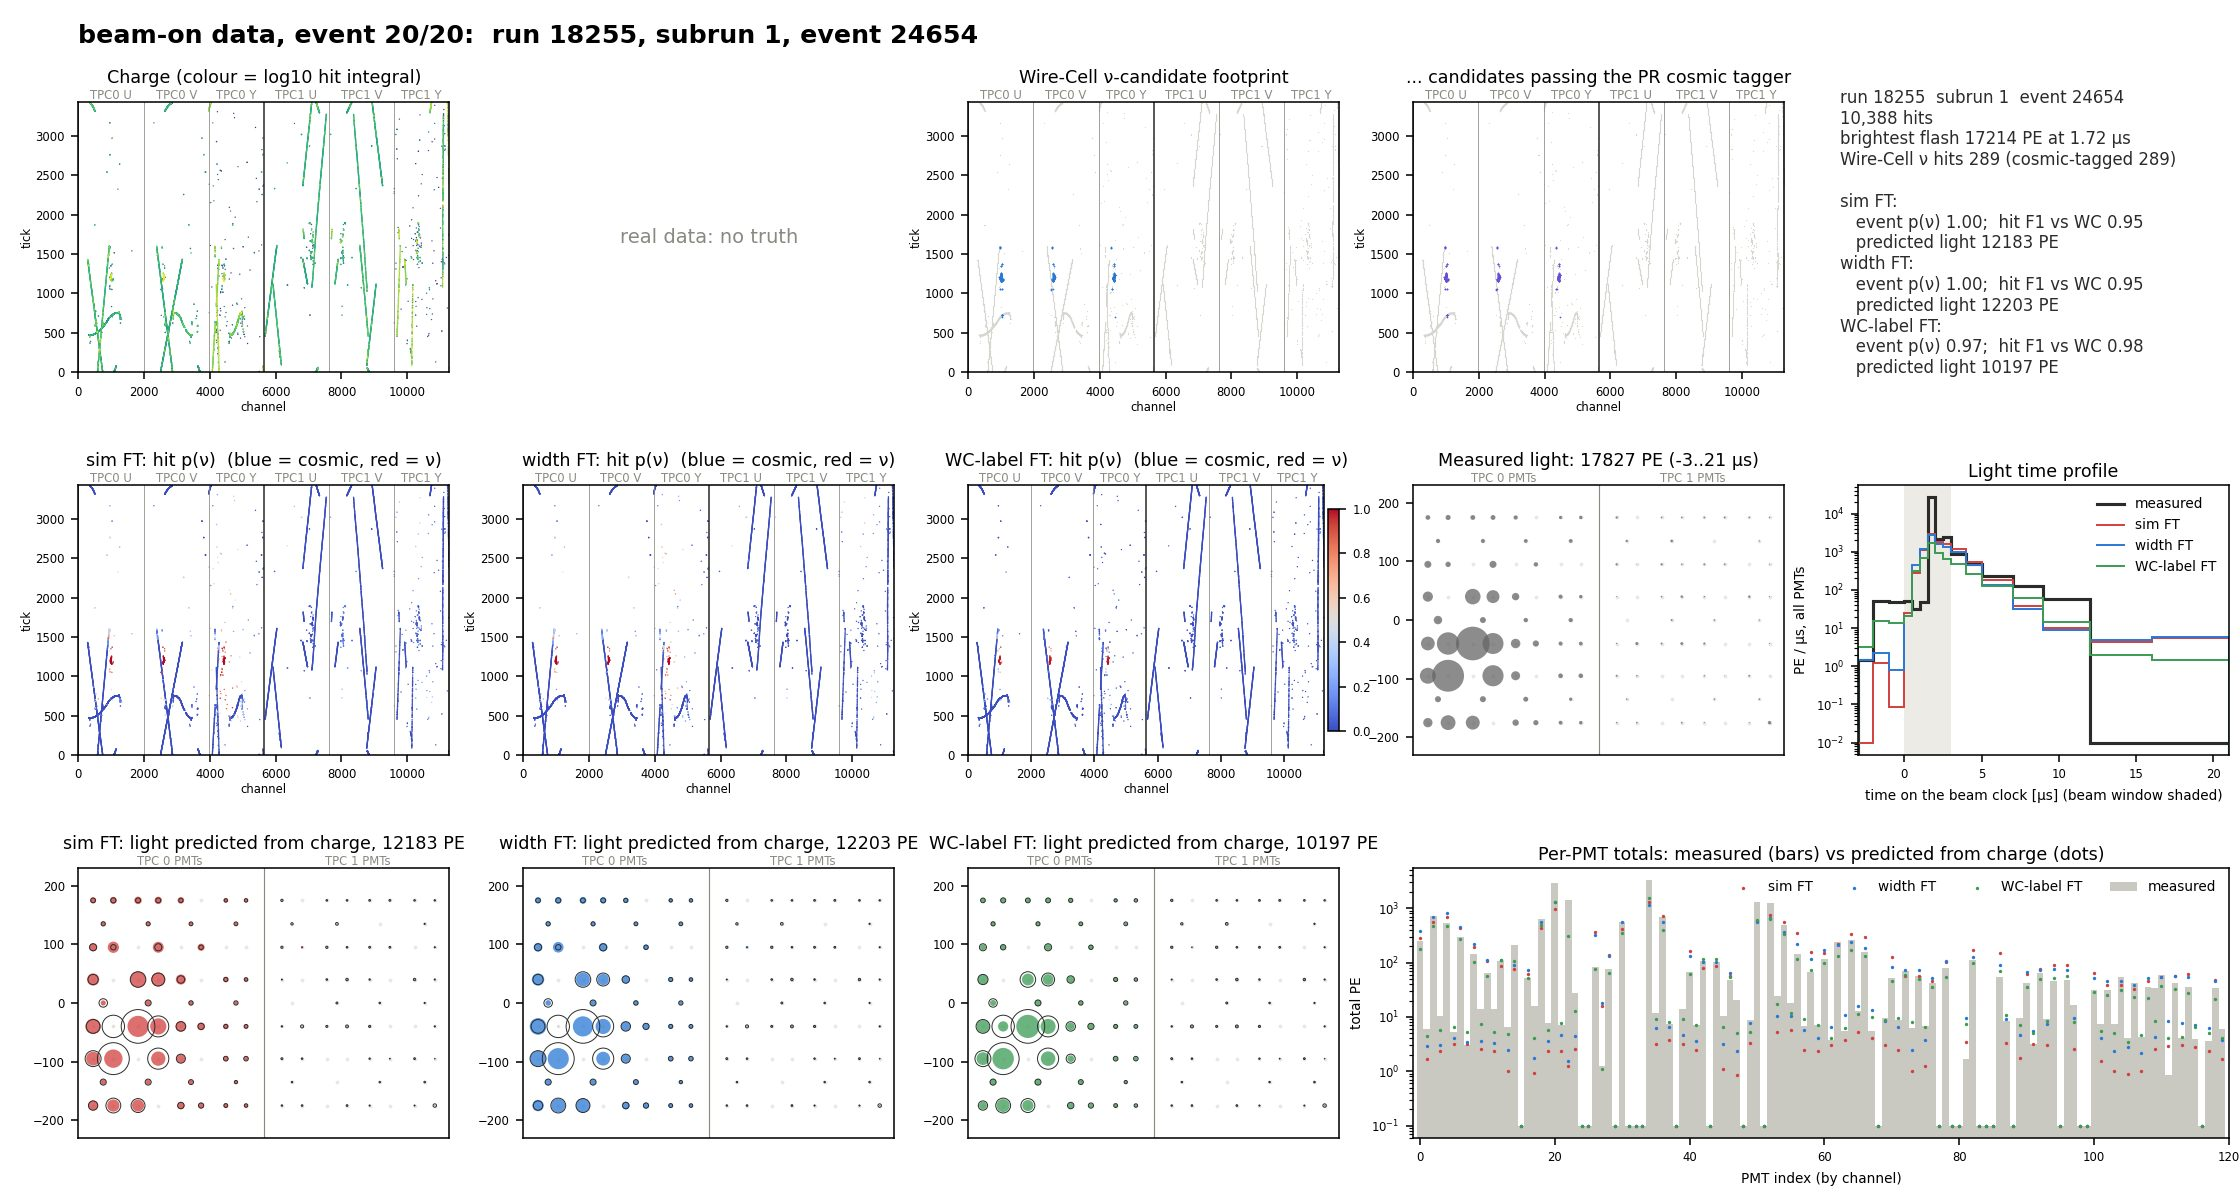
\includegraphics[width=\paperwidth,height=\paperheight,keepaspectratio]{displays/on_19.jpg}}
\end{frame}
\subsection{Off-beam data}
% Off-beam data 1/20: run 18329, subrun 1, event 56813; event p(nu): sim FT 0.00, width FT 0.00, WC-label FT 0.00
\begin{frame}[plain]
  \centering\vspace*{-2pt}
  \makebox[\linewidth][c]{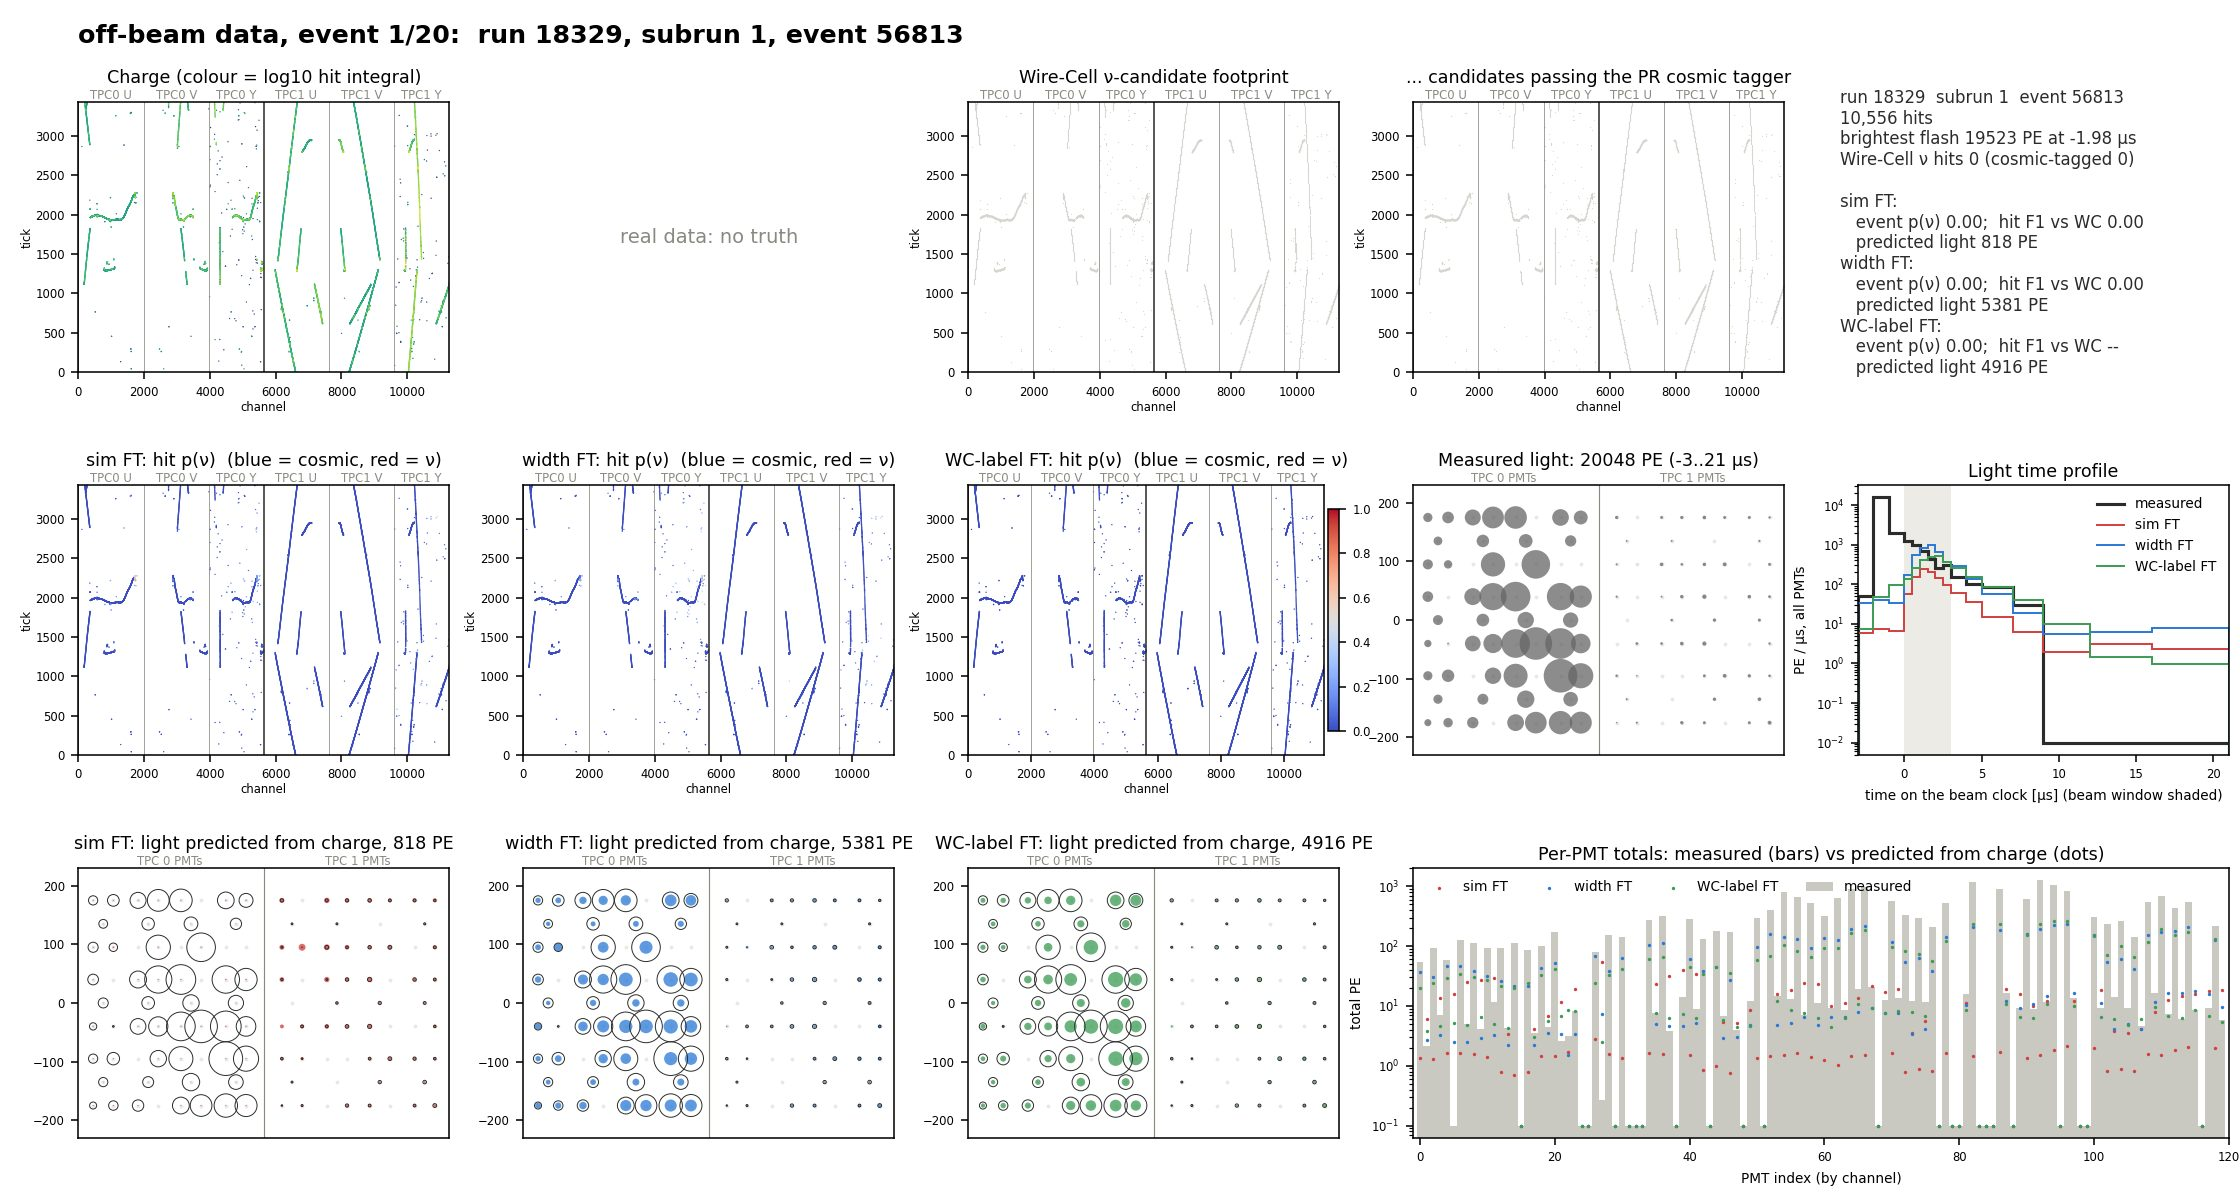
\includegraphics[width=\paperwidth,height=\paperheight,keepaspectratio]{displays/off_00.jpg}}
\end{frame}
% Off-beam data 2/20: run 18355, subrun 1, event 399079; event p(nu): sim FT 0.00, width FT 0.00, WC-label FT 0.00
\begin{frame}[plain]
  \centering\vspace*{-2pt}
  \makebox[\linewidth][c]{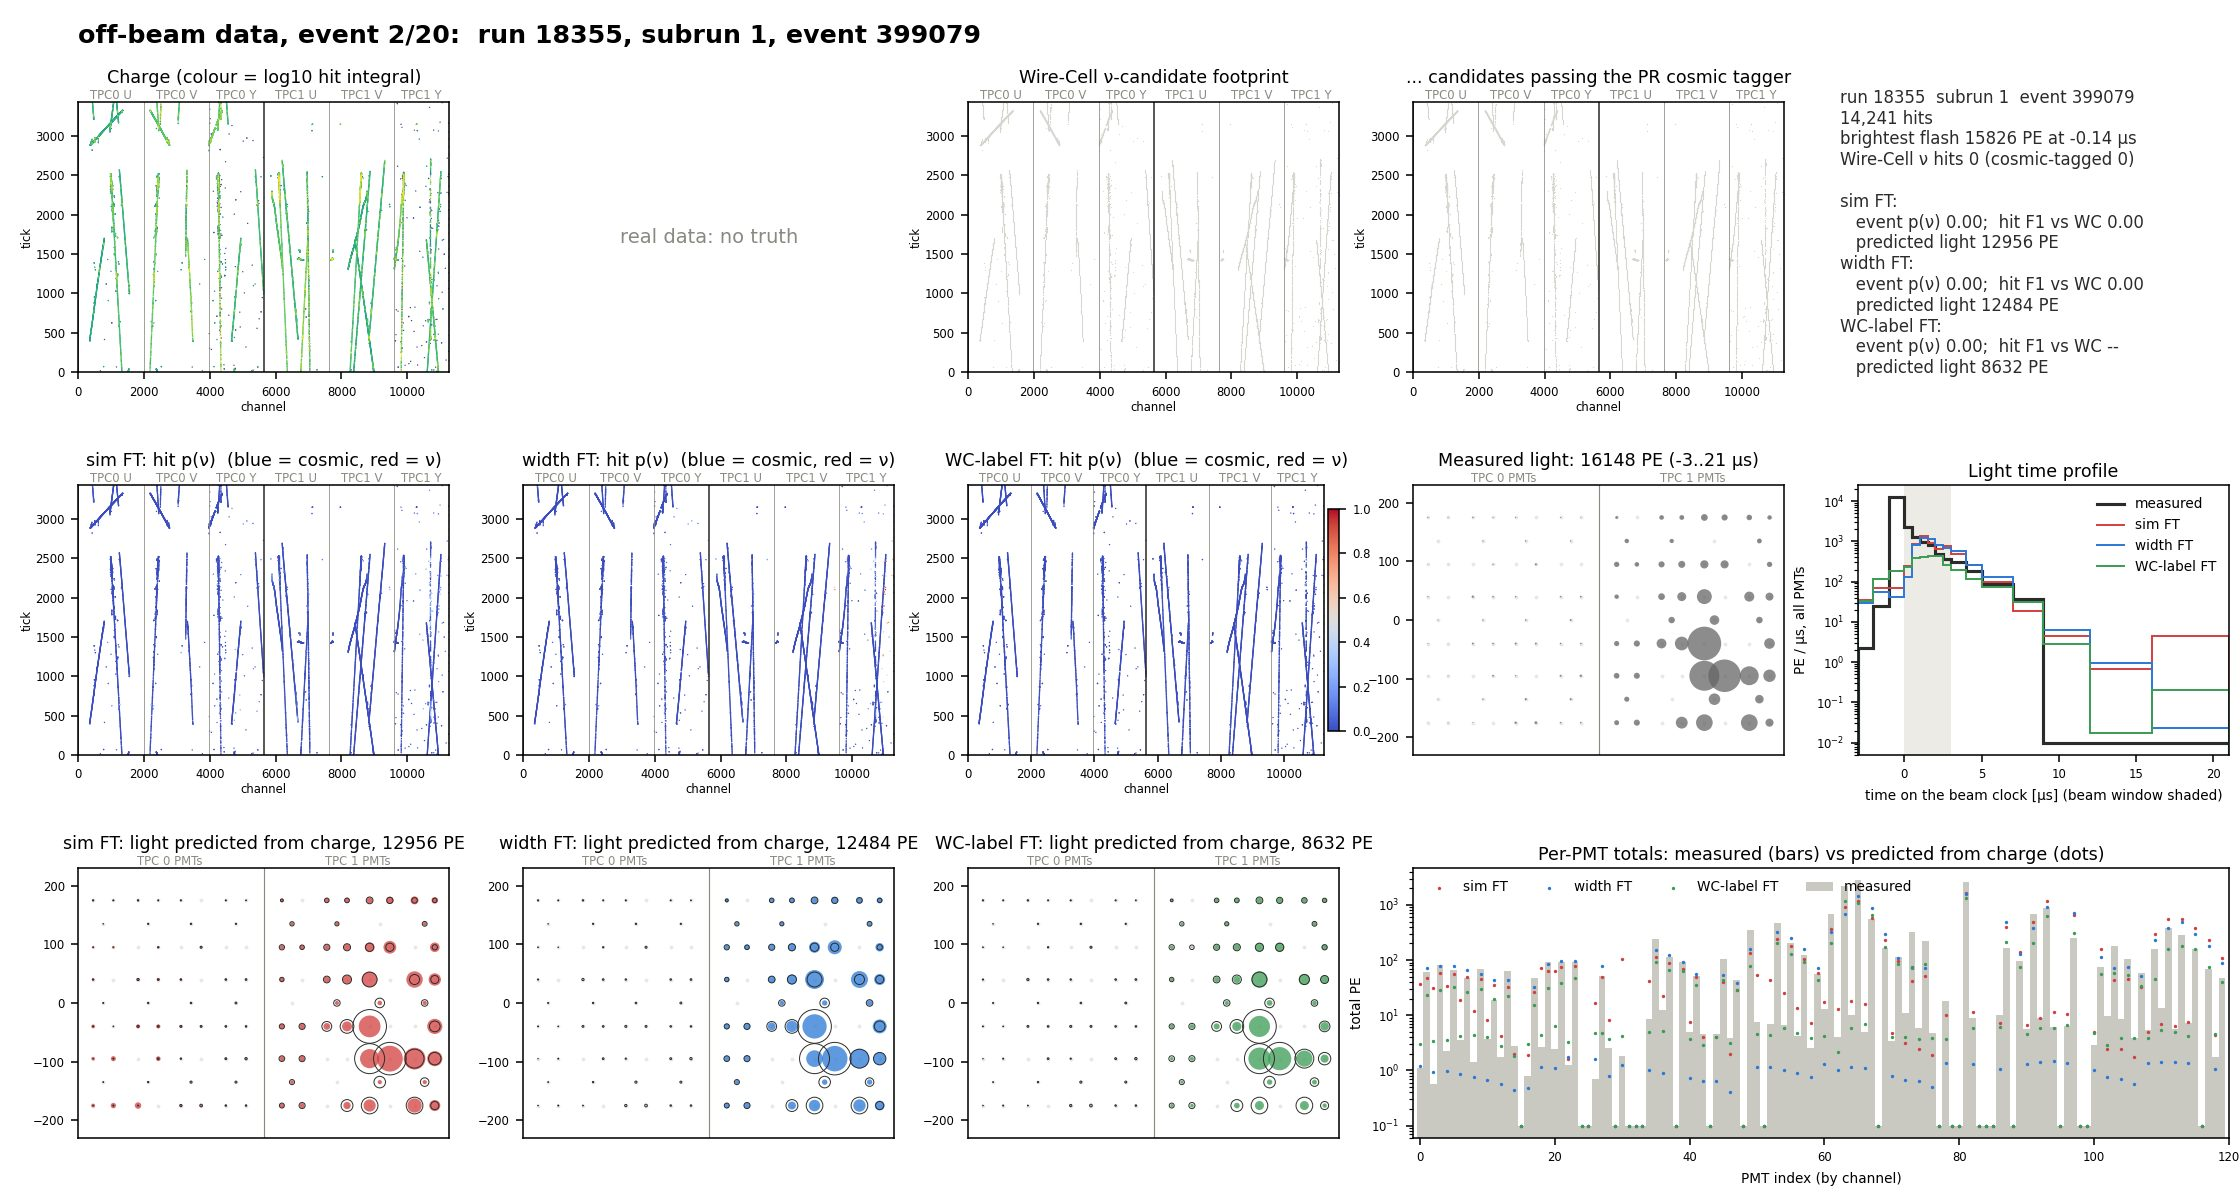
\includegraphics[width=\paperwidth,height=\paperheight,keepaspectratio]{displays/off_01.jpg}}
\end{frame}
% Off-beam data 3/20: run 18468, subrun 1, event 292429; event p(nu): sim FT 0.00, width FT 0.00, WC-label FT 0.12
\begin{frame}[plain]
  \centering\vspace*{-2pt}
  \makebox[\linewidth][c]{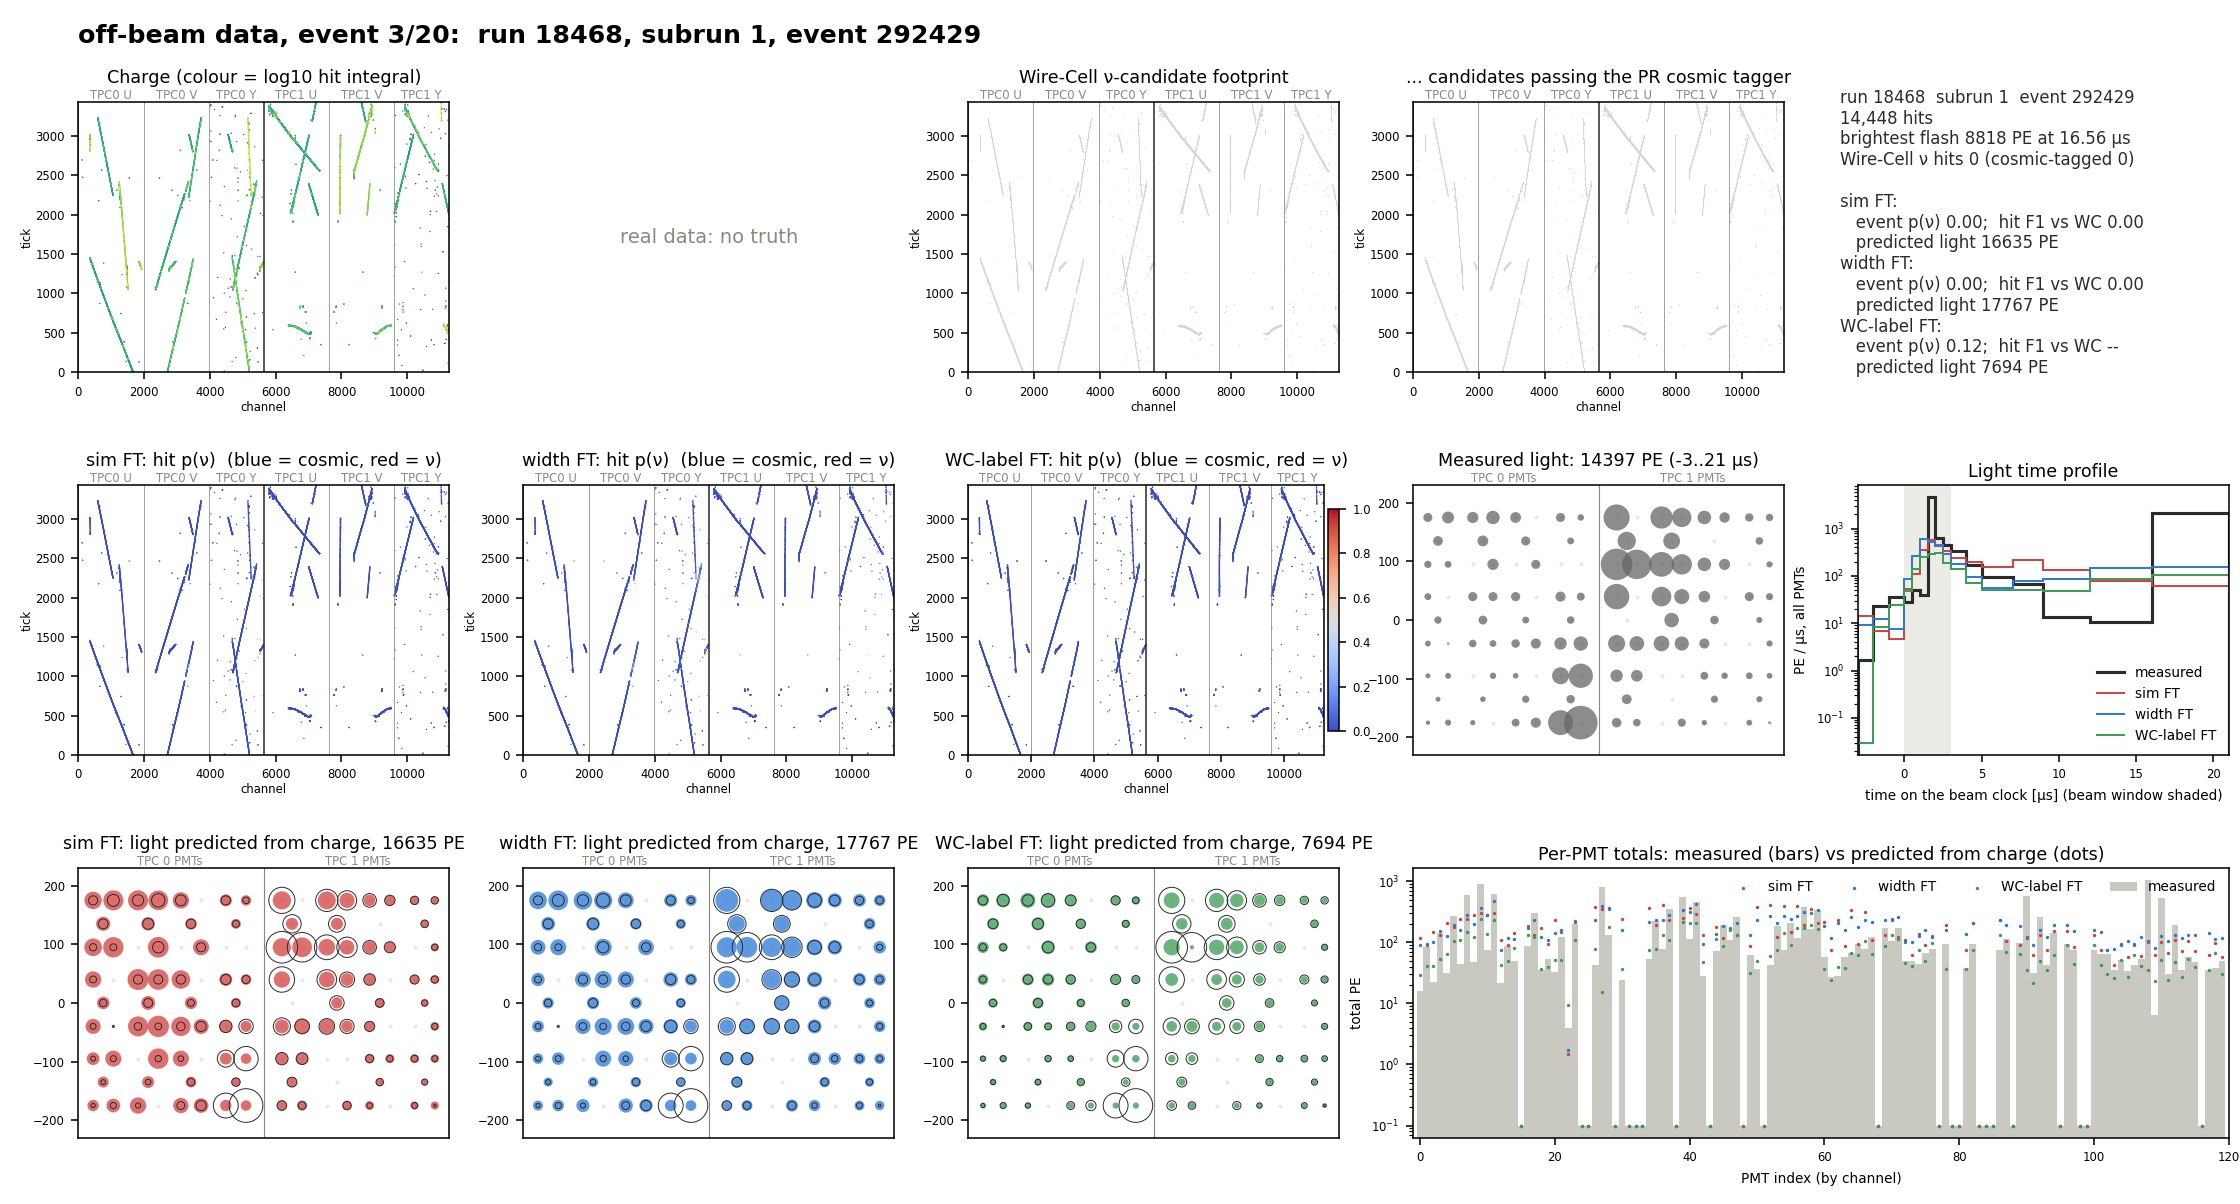
\includegraphics[width=\paperwidth,height=\paperheight,keepaspectratio]{displays/off_02.jpg}}
\end{frame}
% Off-beam data 4/20: run 18275, subrun 1, event 7671; event p(nu): sim FT 0.00, width FT 0.00, WC-label FT 0.03
\begin{frame}[plain]
  \centering\vspace*{-2pt}
  \makebox[\linewidth][c]{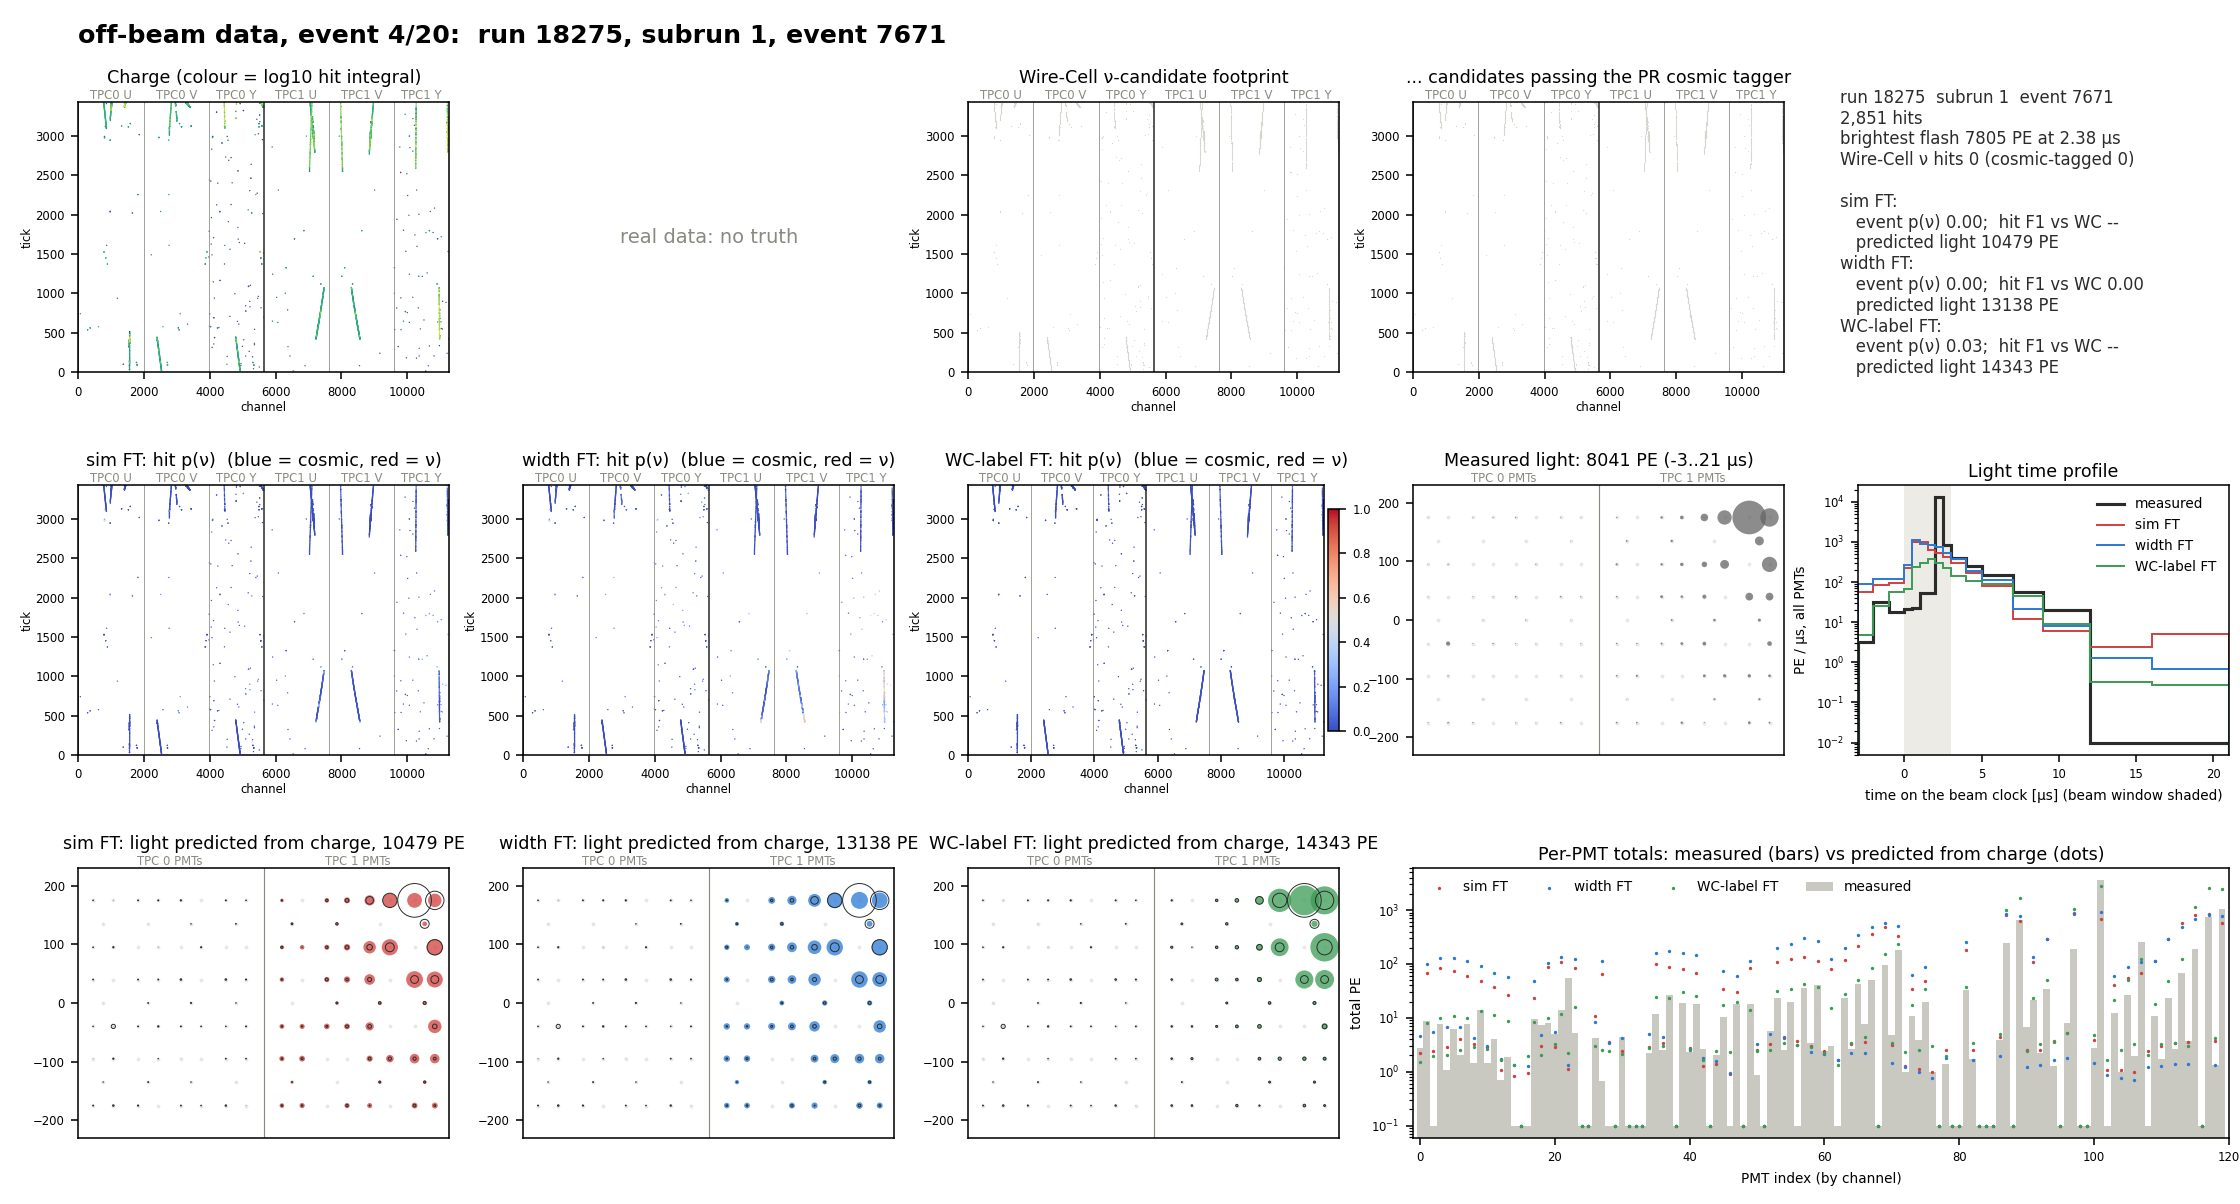
\includegraphics[width=\paperwidth,height=\paperheight,keepaspectratio]{displays/off_03.jpg}}
\end{frame}
% Off-beam data 5/20: run 18484, subrun 1, event 270322; event p(nu): sim FT 0.00, width FT 0.00, WC-label FT 0.00
\begin{frame}[plain]
  \centering\vspace*{-2pt}
  \makebox[\linewidth][c]{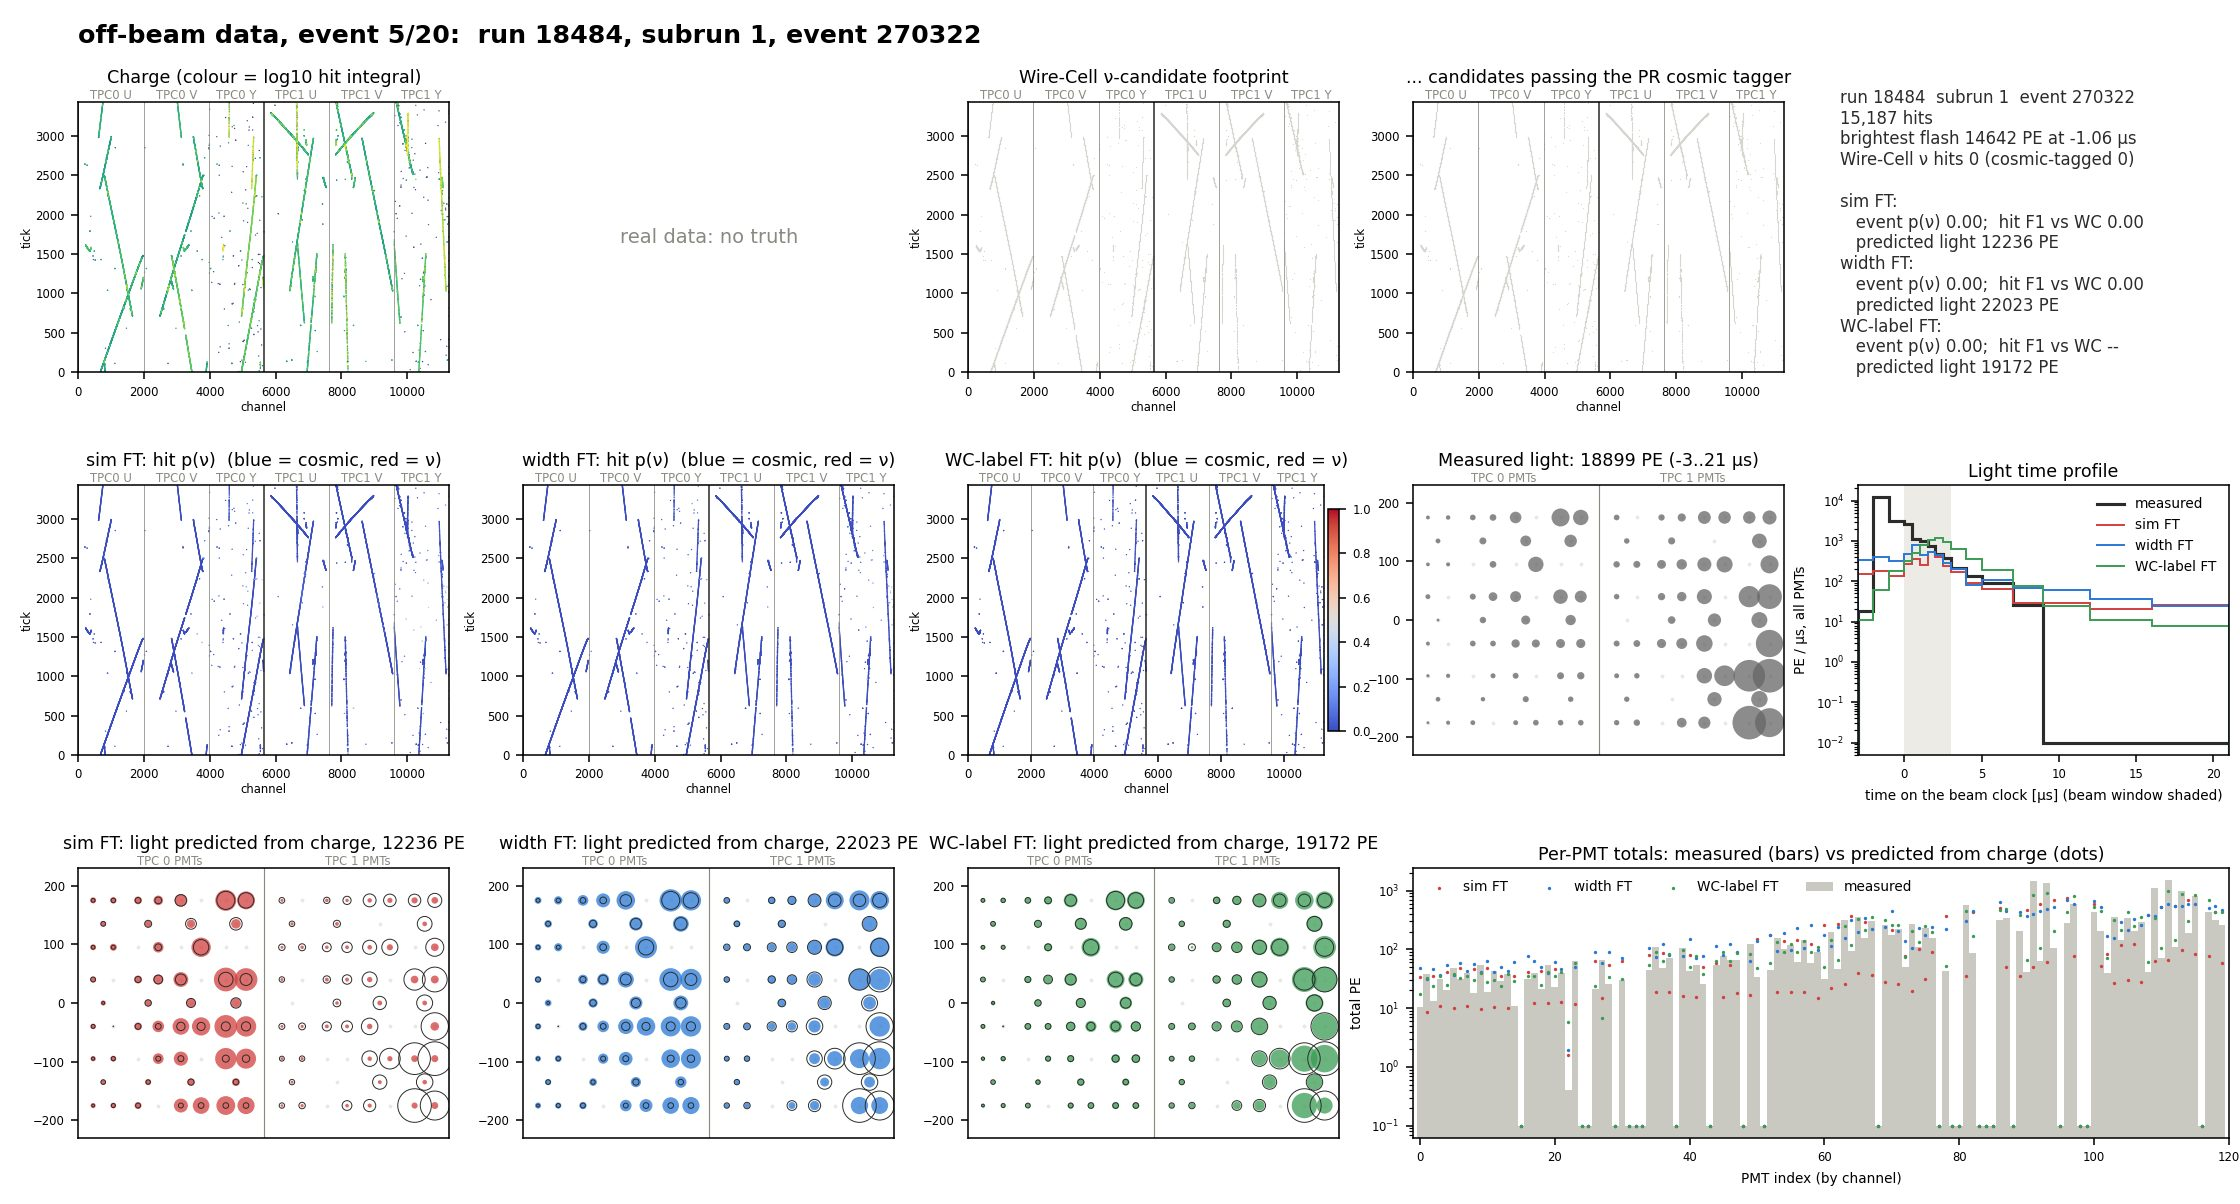
\includegraphics[width=\paperwidth,height=\paperheight,keepaspectratio]{displays/off_04.jpg}}
\end{frame}
% Off-beam data 6/20: run 18308, subrun 1, event 54357; event p(nu): sim FT 0.00, width FT 0.00, WC-label FT 0.00
\begin{frame}[plain]
  \centering\vspace*{-2pt}
  \makebox[\linewidth][c]{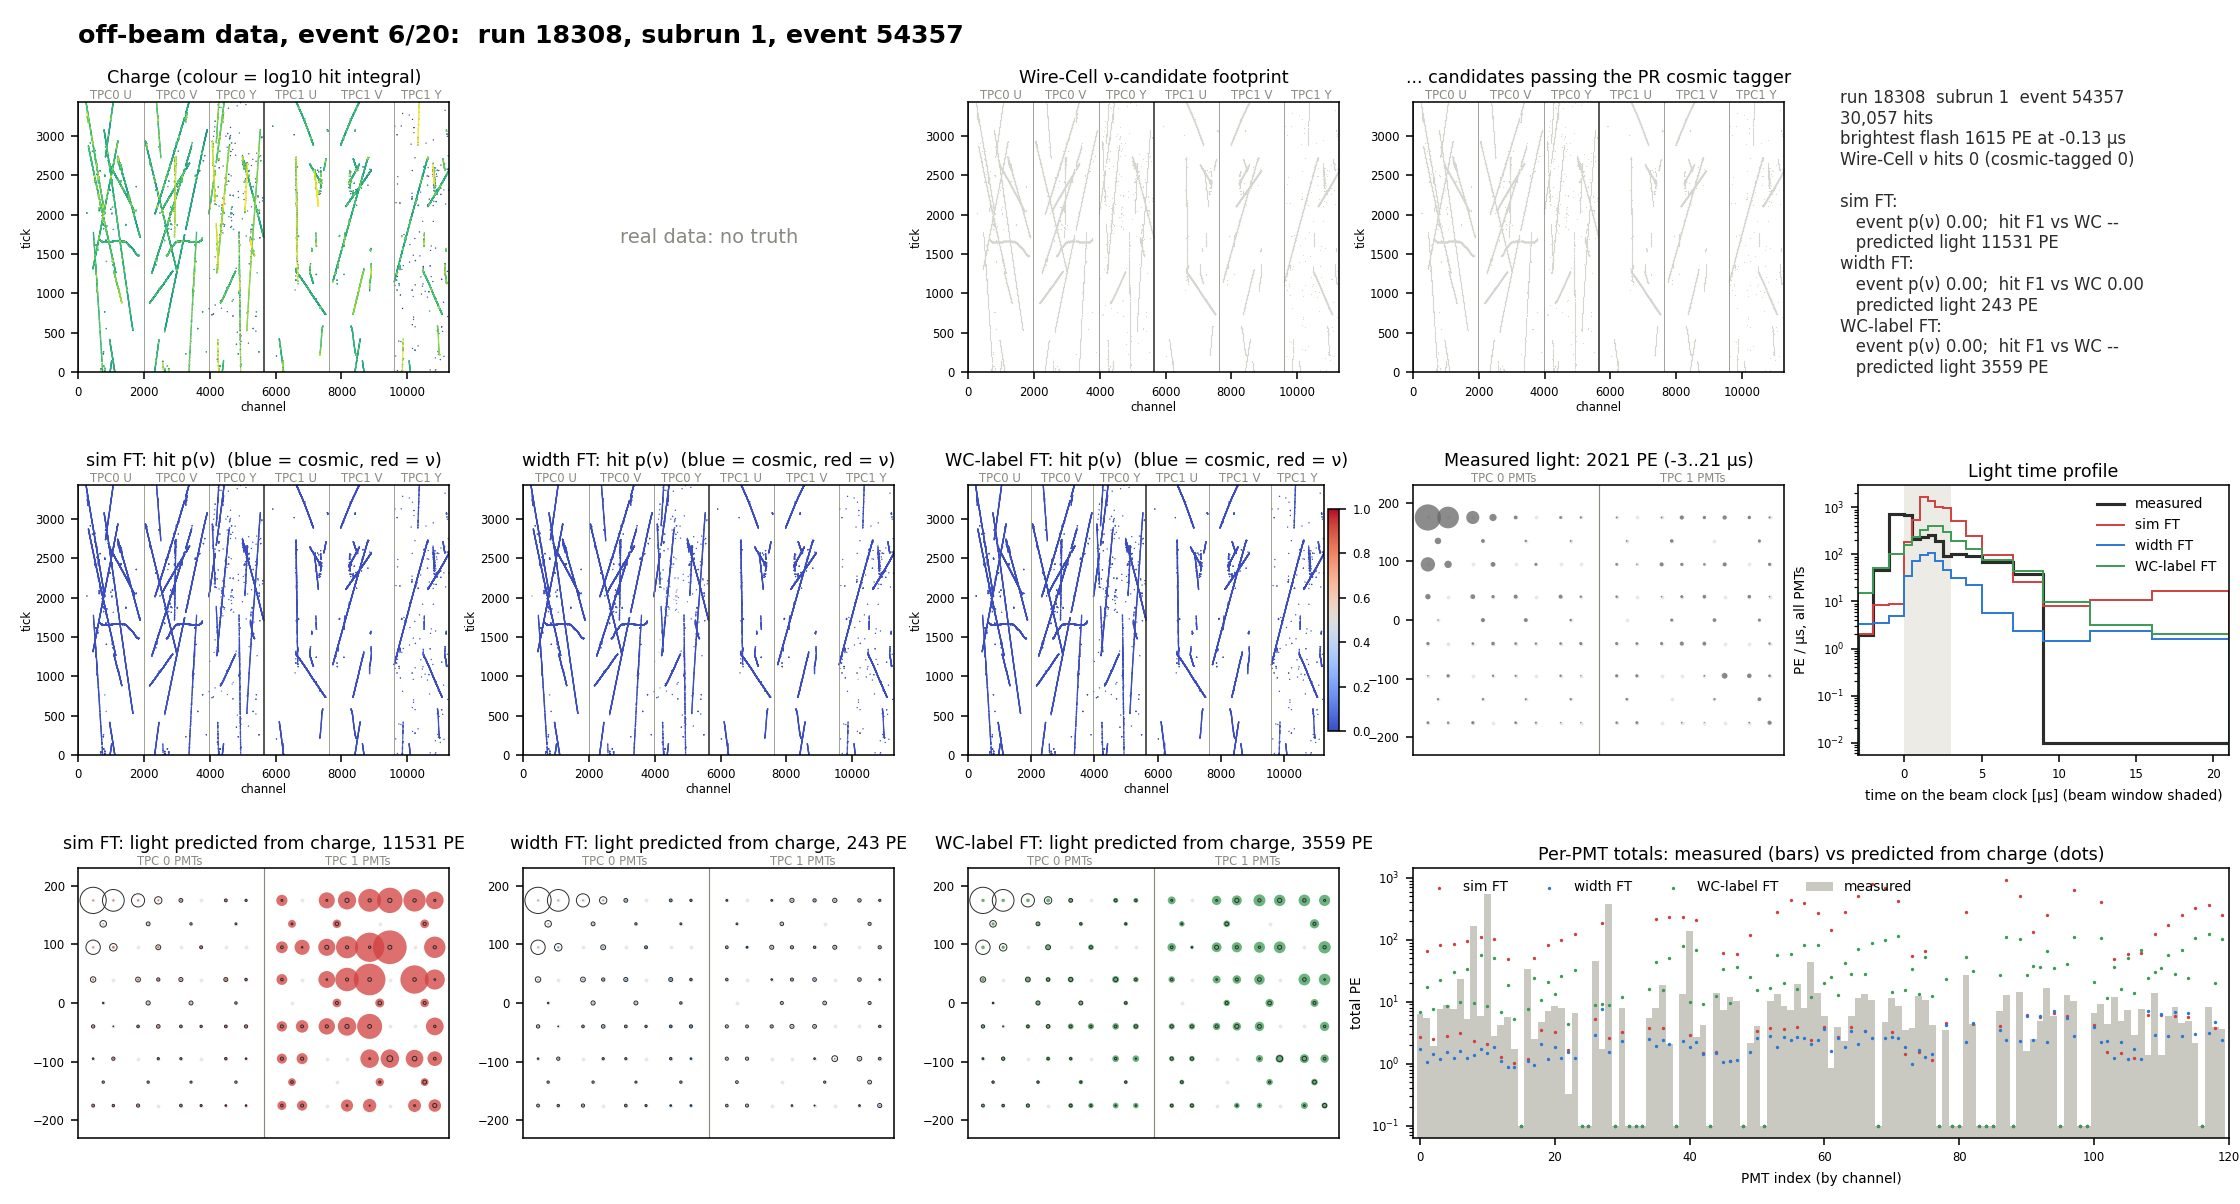
\includegraphics[width=\paperwidth,height=\paperheight,keepaspectratio]{displays/off_05.jpg}}
\end{frame}
% Off-beam data 7/20: run 18329, subrun 1, event 439641; event p(nu): sim FT 0.11, width FT 0.00, WC-label FT 0.03
\begin{frame}[plain]
  \centering\vspace*{-2pt}
  \makebox[\linewidth][c]{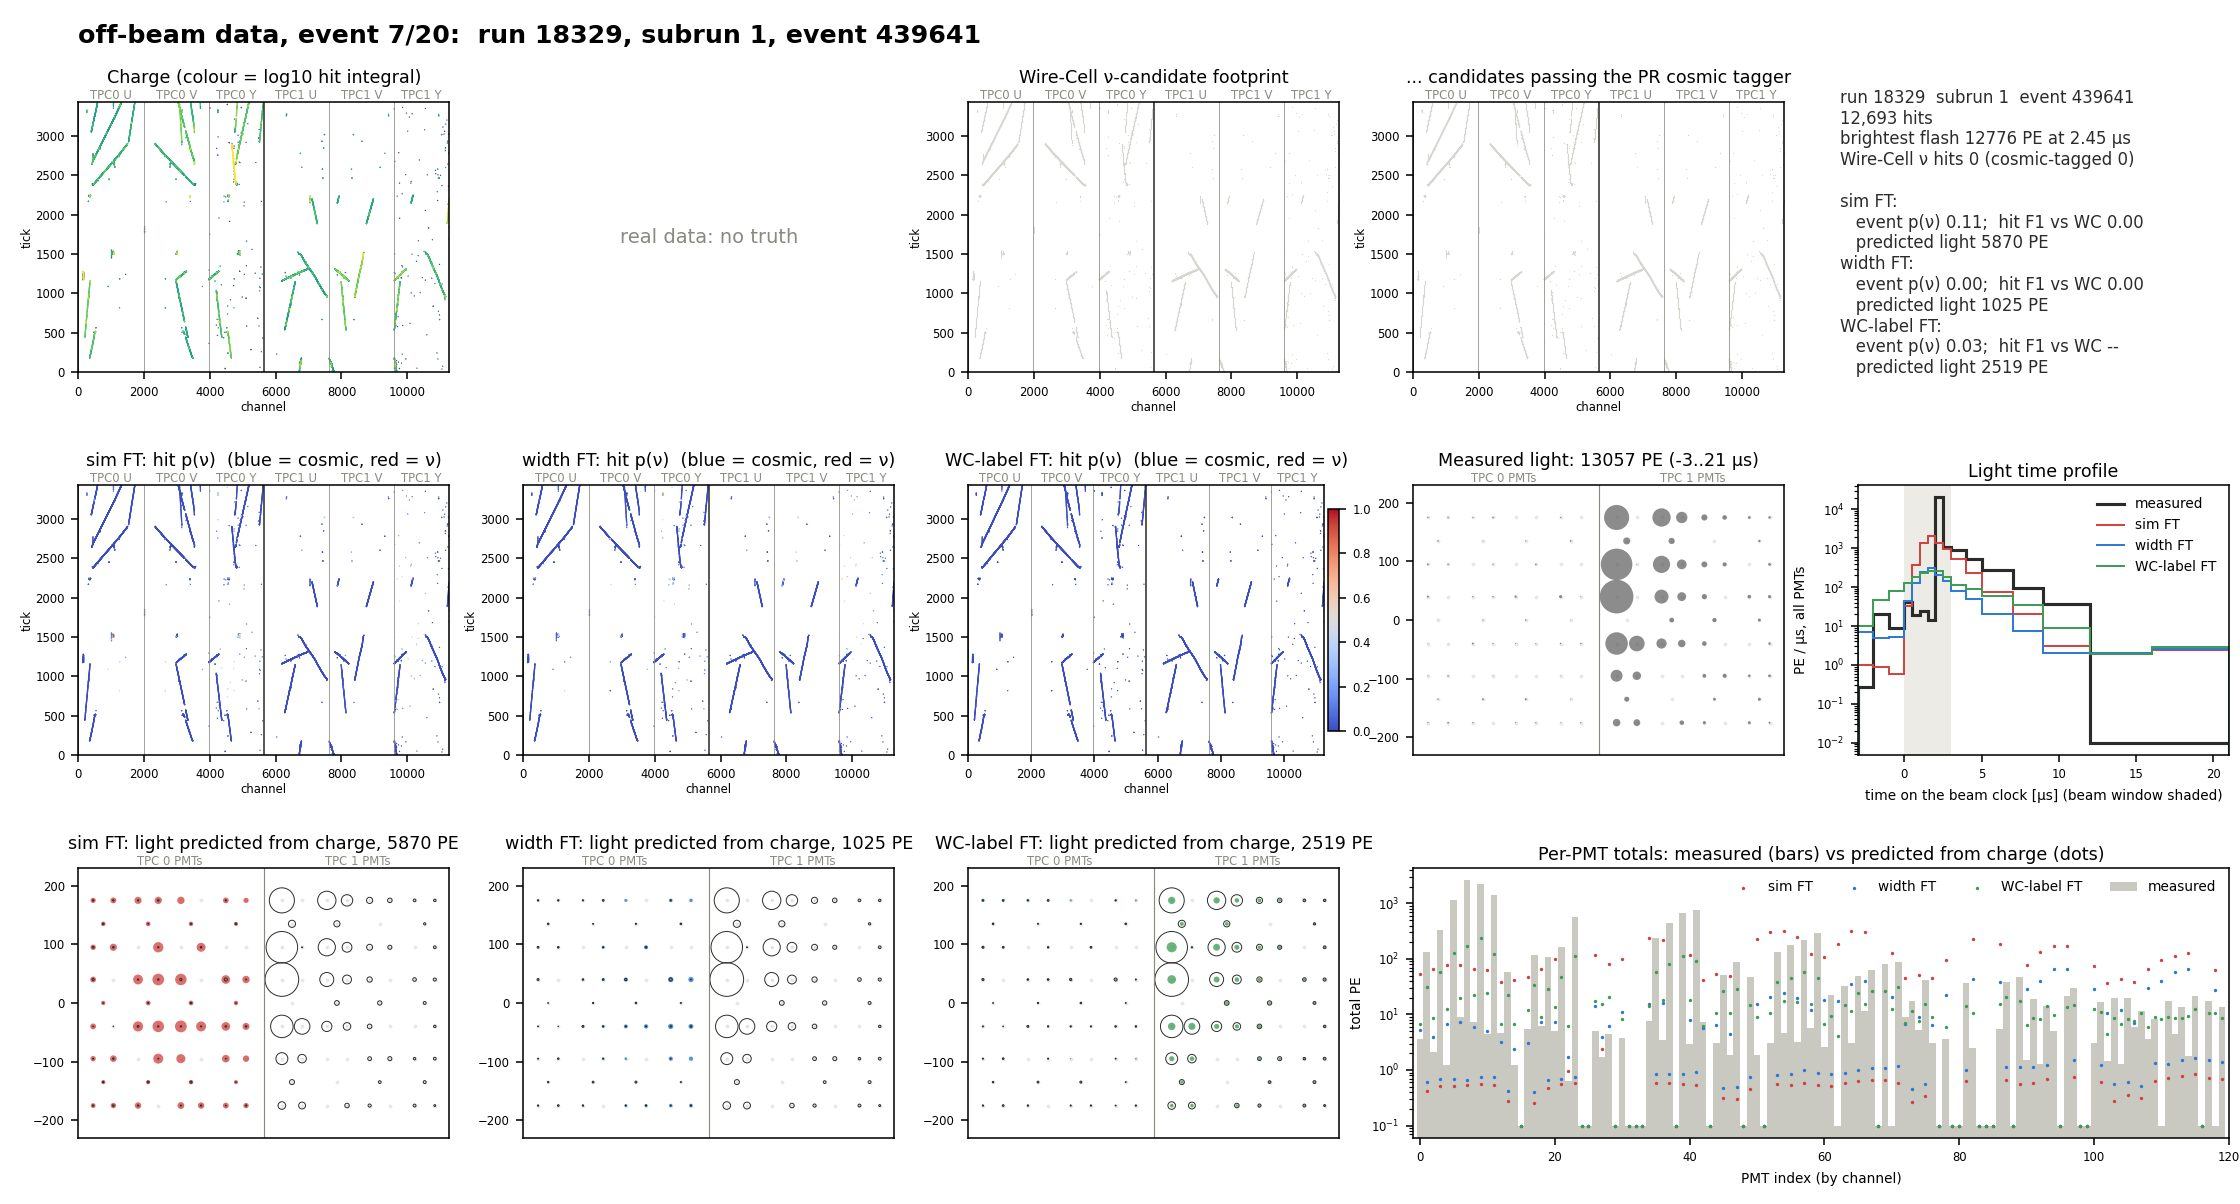
\includegraphics[width=\paperwidth,height=\paperheight,keepaspectratio]{displays/off_06.jpg}}
\end{frame}
% Off-beam data 8/20: run 18250, subrun 1, event 102489; event p(nu): sim FT 0.00, width FT 0.00, WC-label FT 0.03
\begin{frame}[plain]
  \centering\vspace*{-2pt}
  \makebox[\linewidth][c]{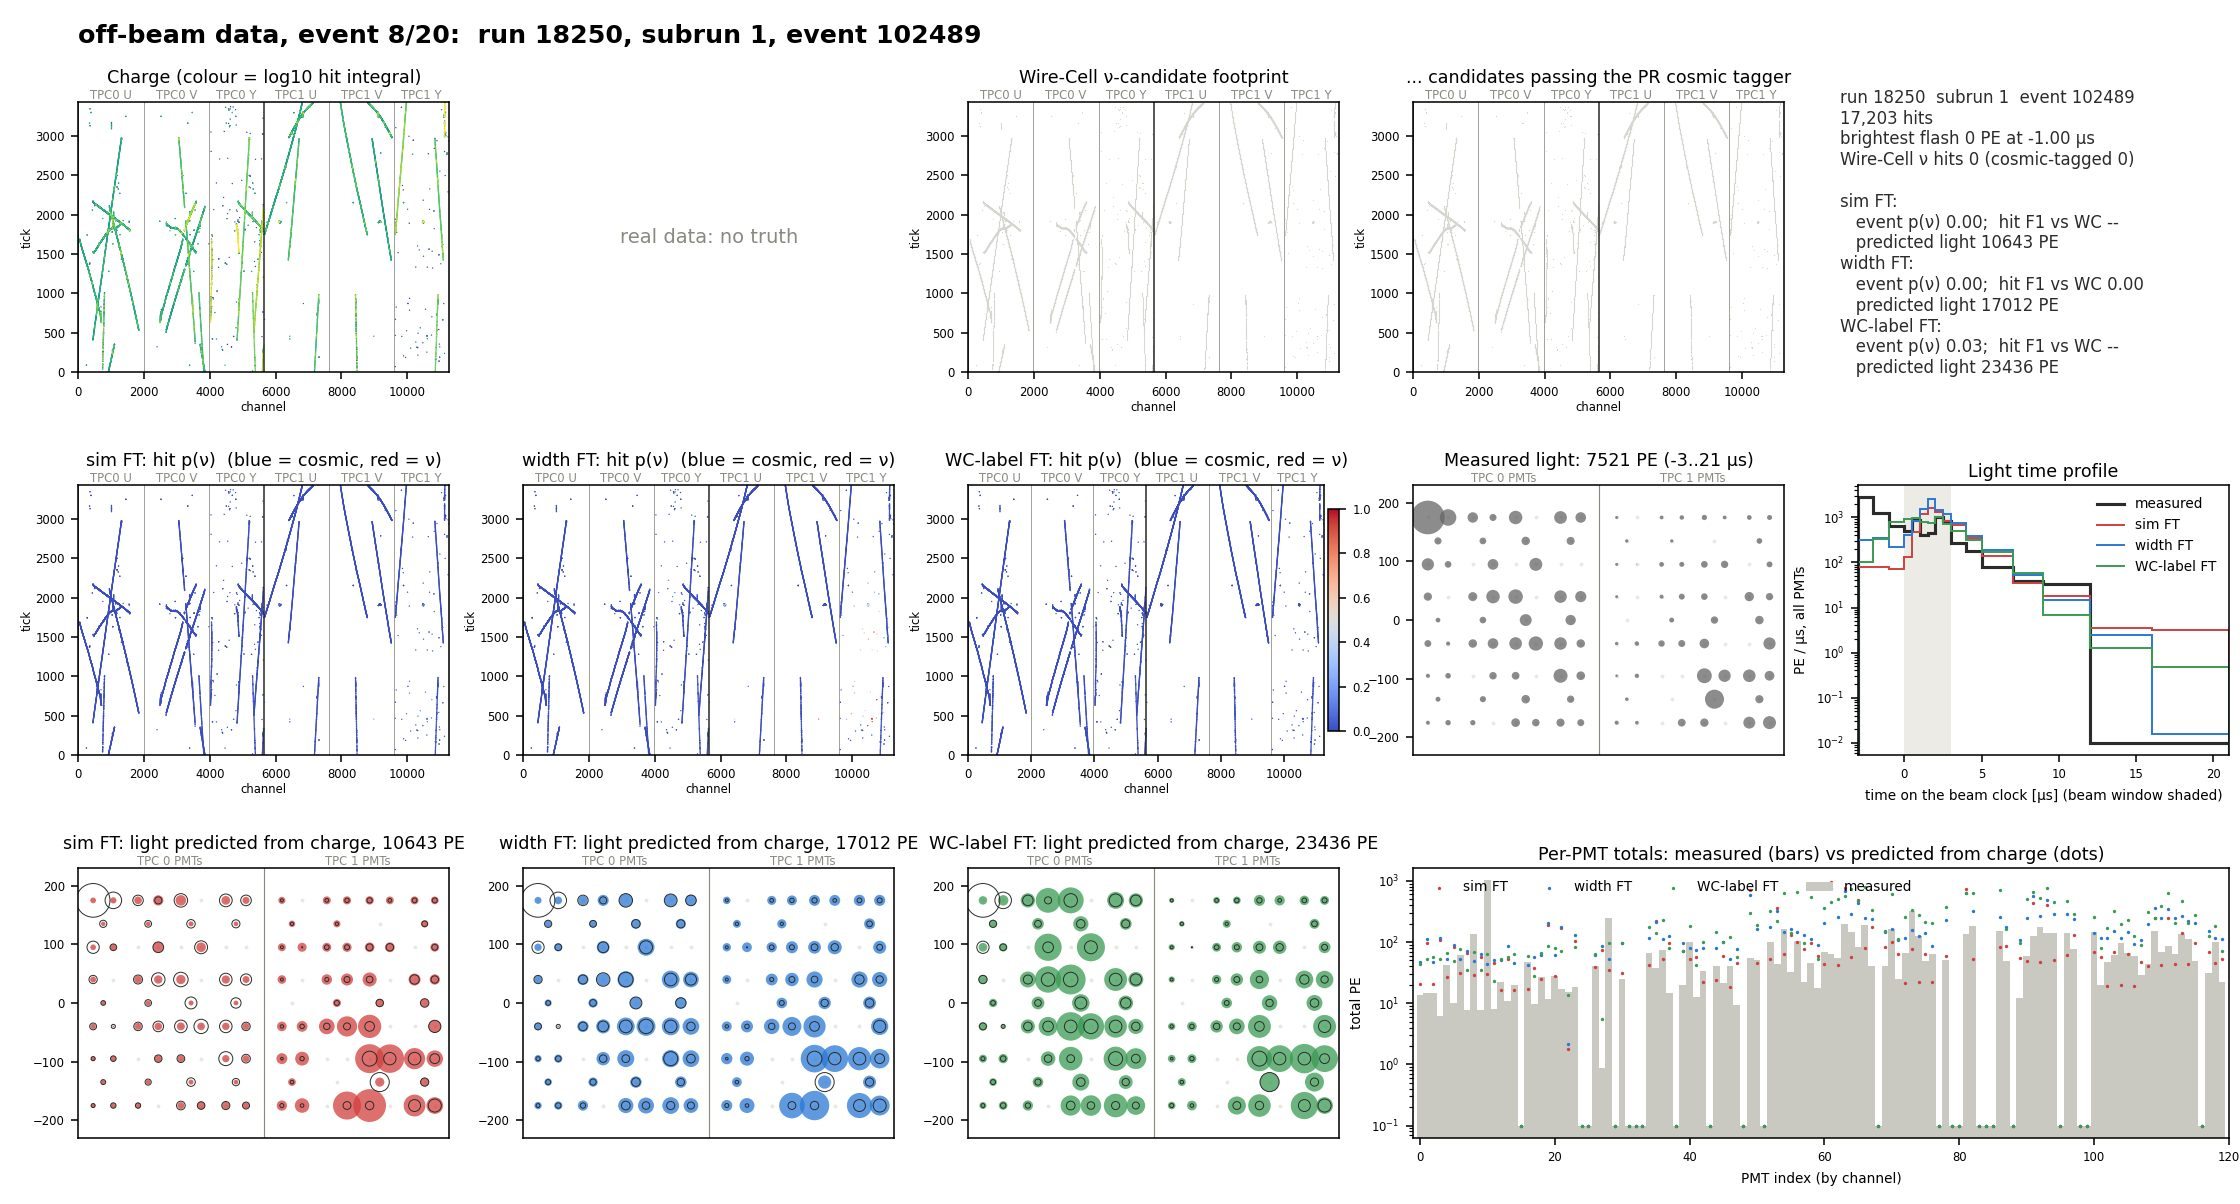
\includegraphics[width=\paperwidth,height=\paperheight,keepaspectratio]{displays/off_07.jpg}}
\end{frame}
% Off-beam data 9/20: run 18365, subrun 1, event 245600; event p(nu): sim FT 0.00, width FT 0.00, WC-label FT 0.05
\begin{frame}[plain]
  \centering\vspace*{-2pt}
  \makebox[\linewidth][c]{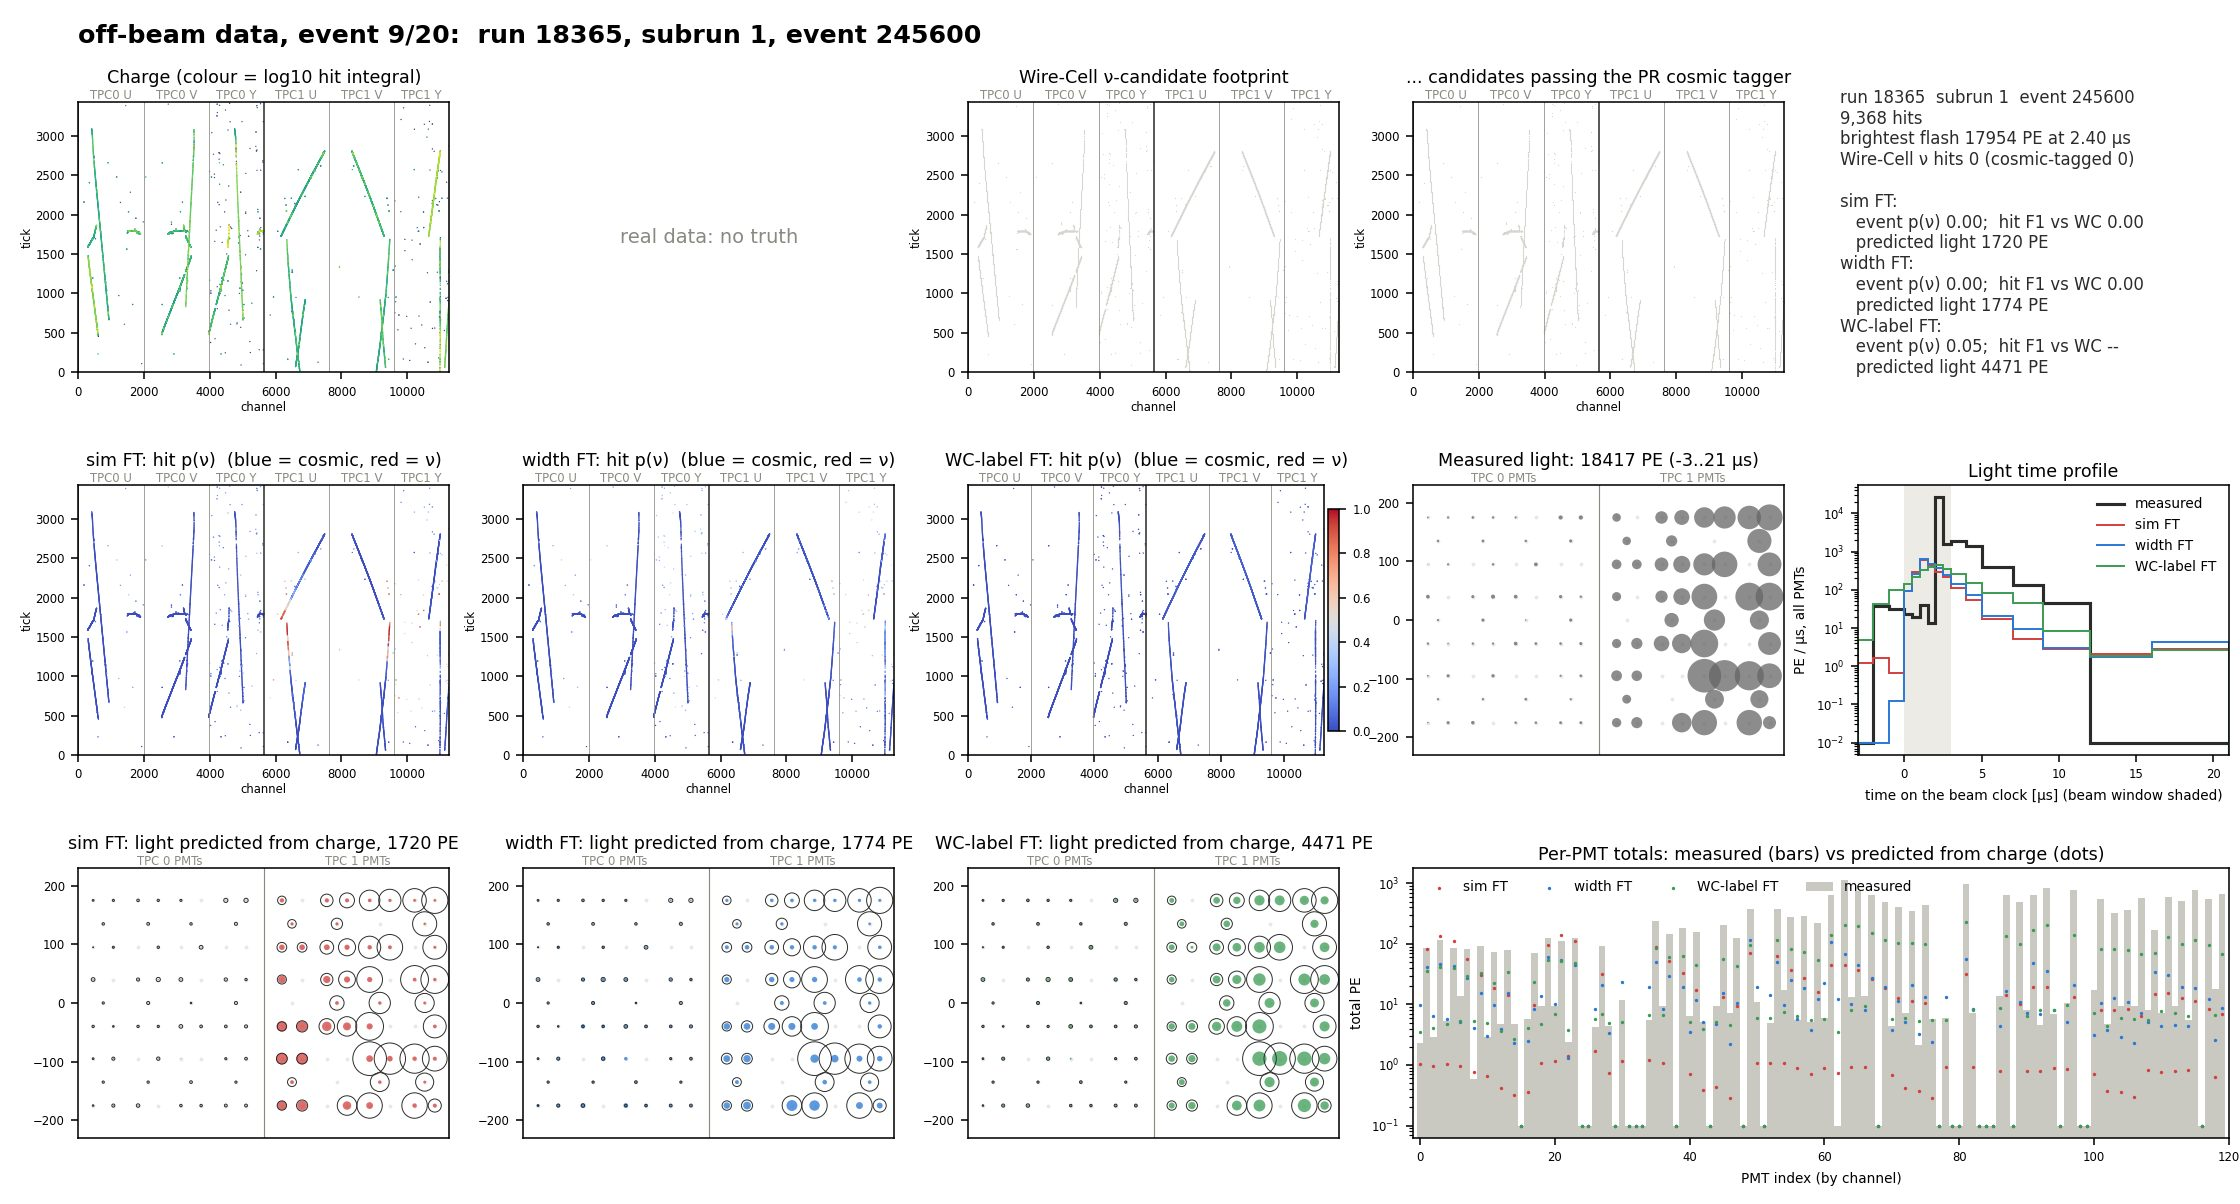
\includegraphics[width=\paperwidth,height=\paperheight,keepaspectratio]{displays/off_08.jpg}}
\end{frame}
% Off-beam data 10/20: run 18509, subrun 1, event 2583; event p(nu): sim FT 0.00, width FT 0.00, WC-label FT 0.15
\begin{frame}[plain]
  \centering\vspace*{-2pt}
  \makebox[\linewidth][c]{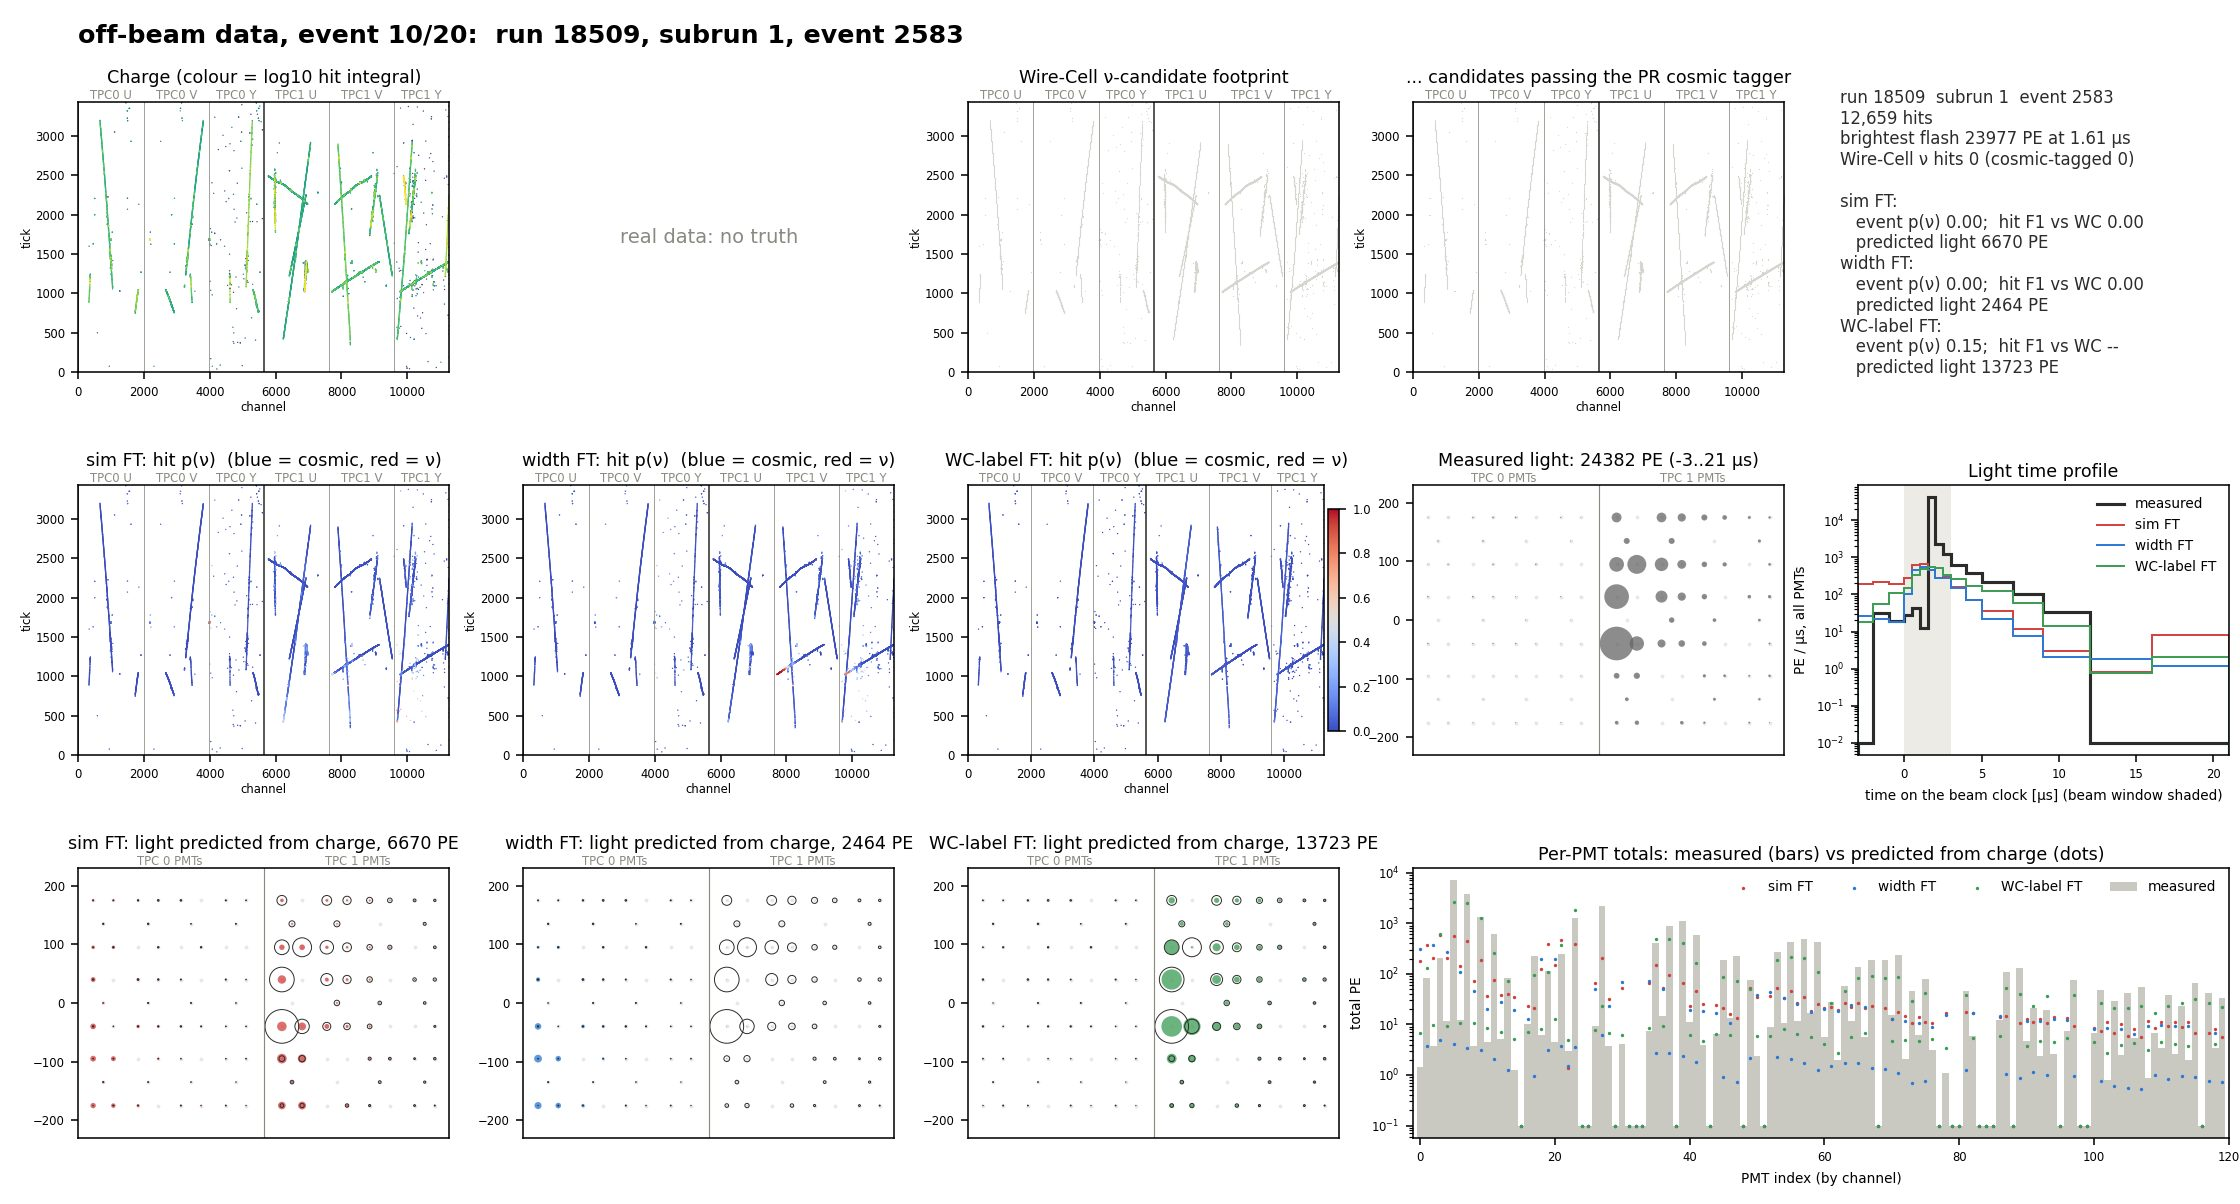
\includegraphics[width=\paperwidth,height=\paperheight,keepaspectratio]{displays/off_09.jpg}}
\end{frame}
% Off-beam data 11/20: run 18259, subrun 1, event 133561; event p(nu): sim FT 0.00, width FT 0.00, WC-label FT 0.00
\begin{frame}[plain]
  \centering\vspace*{-2pt}
  \makebox[\linewidth][c]{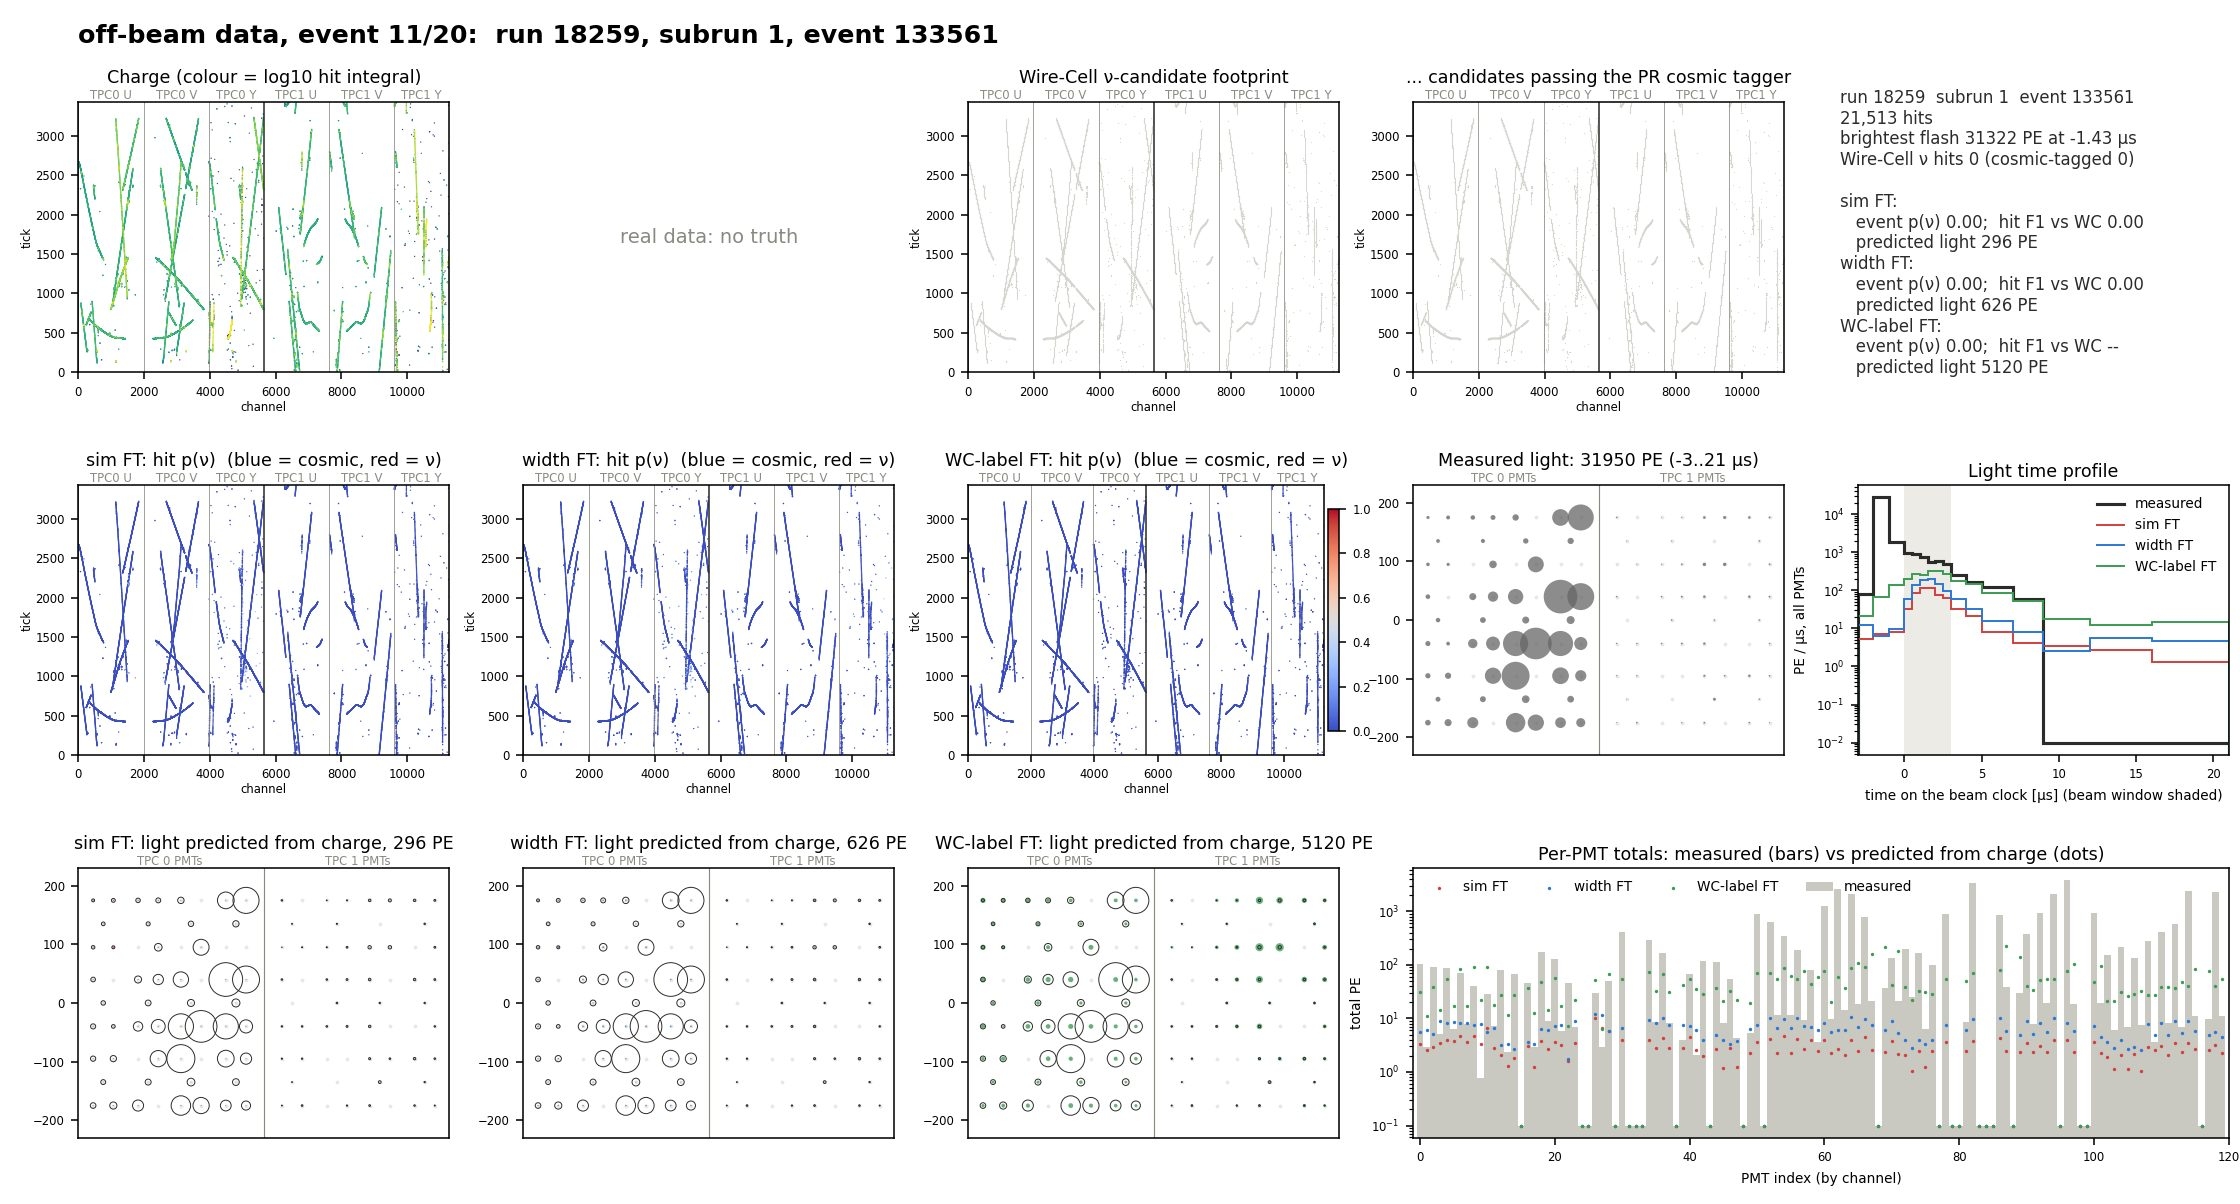
\includegraphics[width=\paperwidth,height=\paperheight,keepaspectratio]{displays/off_10.jpg}}
\end{frame}
% Off-beam data 12/20: run 18334, subrun 1, event 105361; event p(nu): sim FT 0.00, width FT 0.00, WC-label FT 0.09
\begin{frame}[plain]
  \centering\vspace*{-2pt}
  \makebox[\linewidth][c]{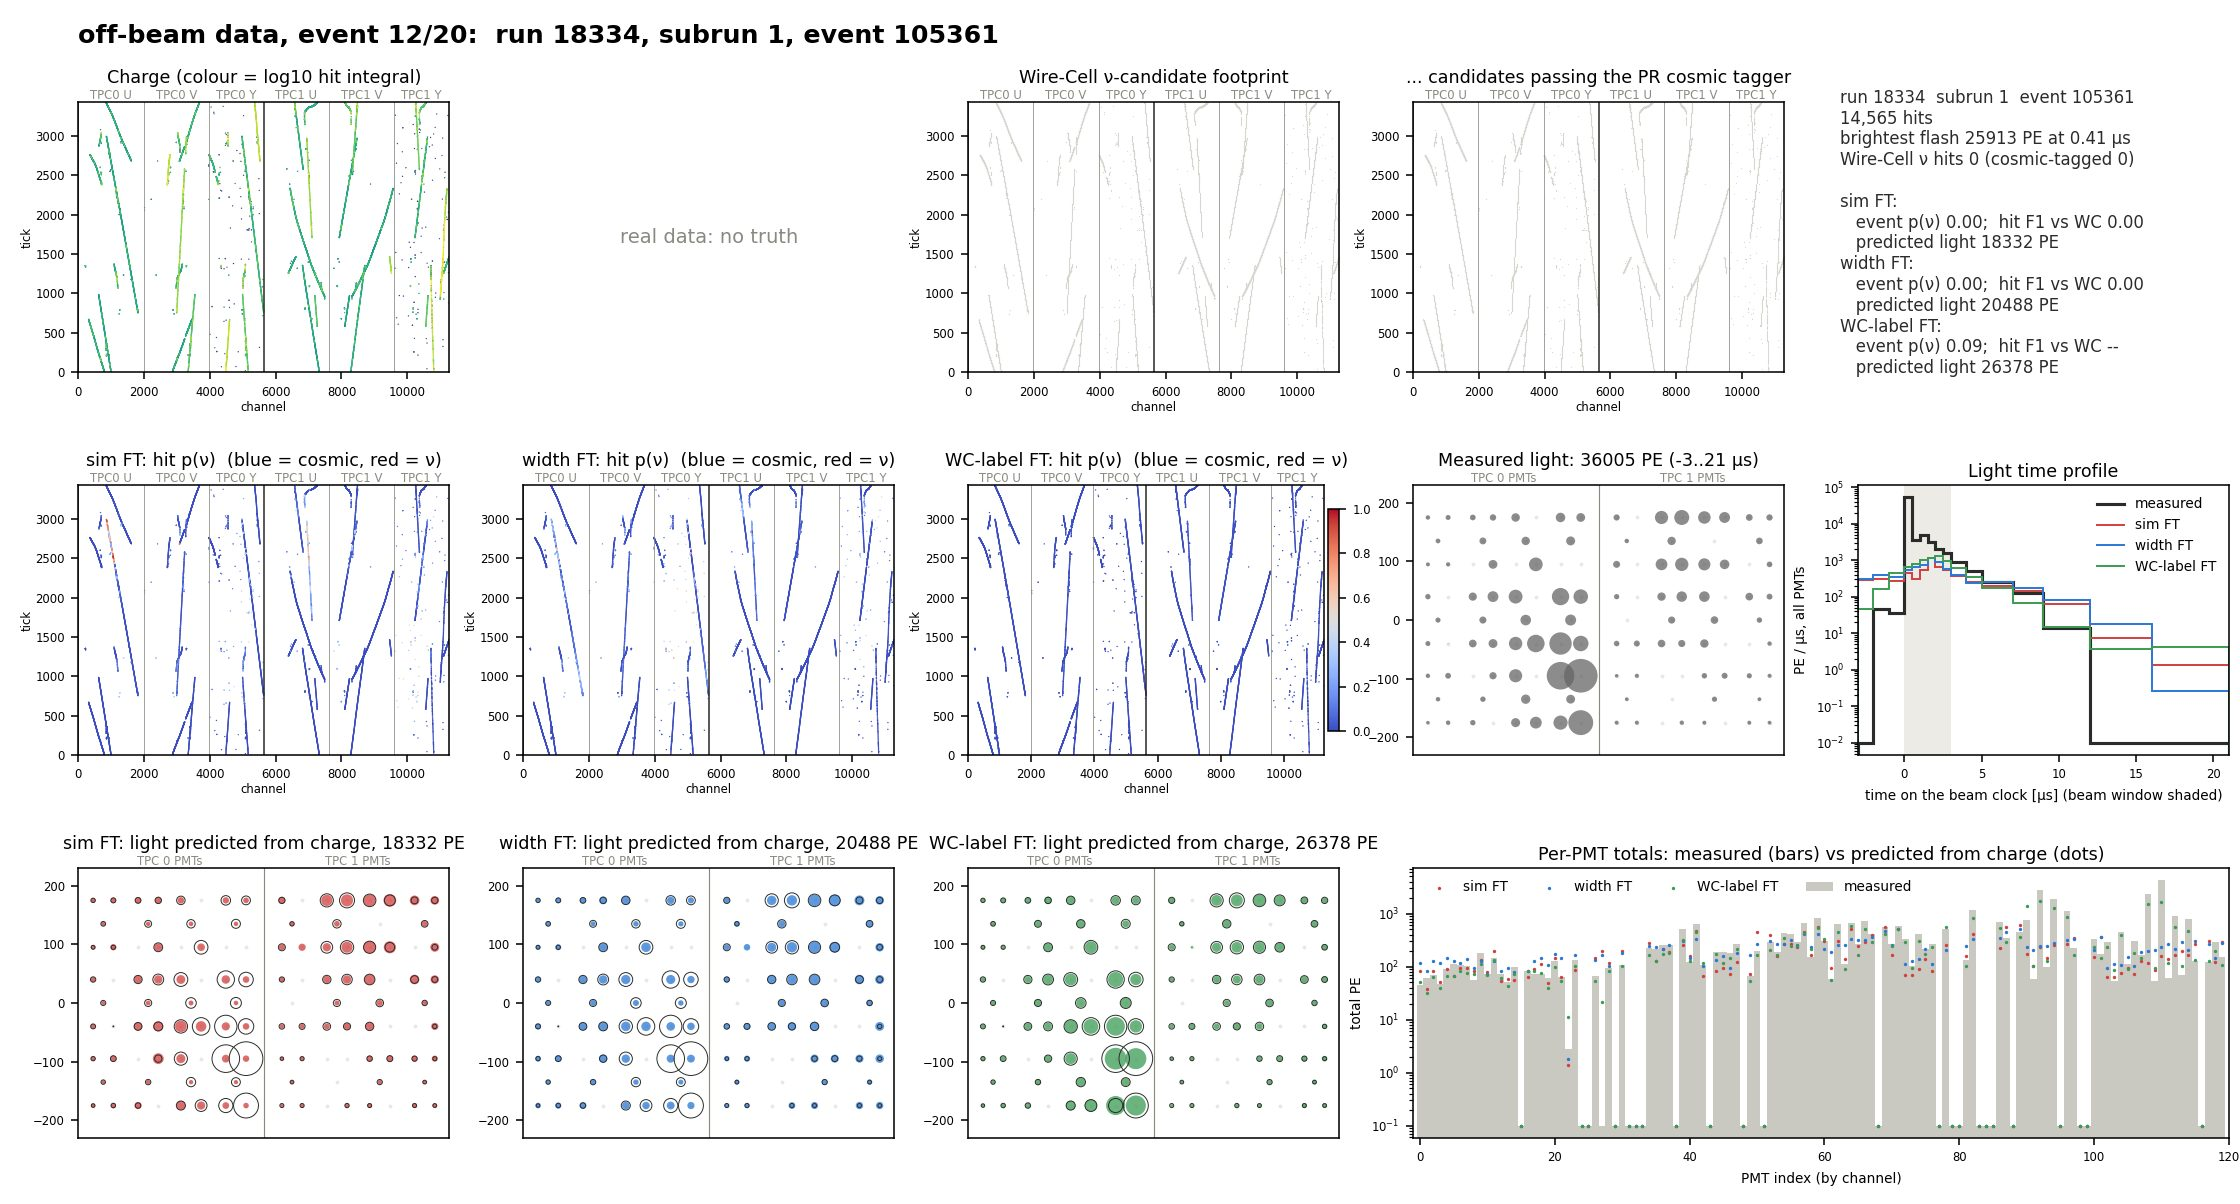
\includegraphics[width=\paperwidth,height=\paperheight,keepaspectratio]{displays/off_11.jpg}}
\end{frame}
% Off-beam data 13/20: run 18326, subrun 1, event 145516; event p(nu): sim FT 0.00, width FT 0.00, WC-label FT 0.04
\begin{frame}[plain]
  \centering\vspace*{-2pt}
  \makebox[\linewidth][c]{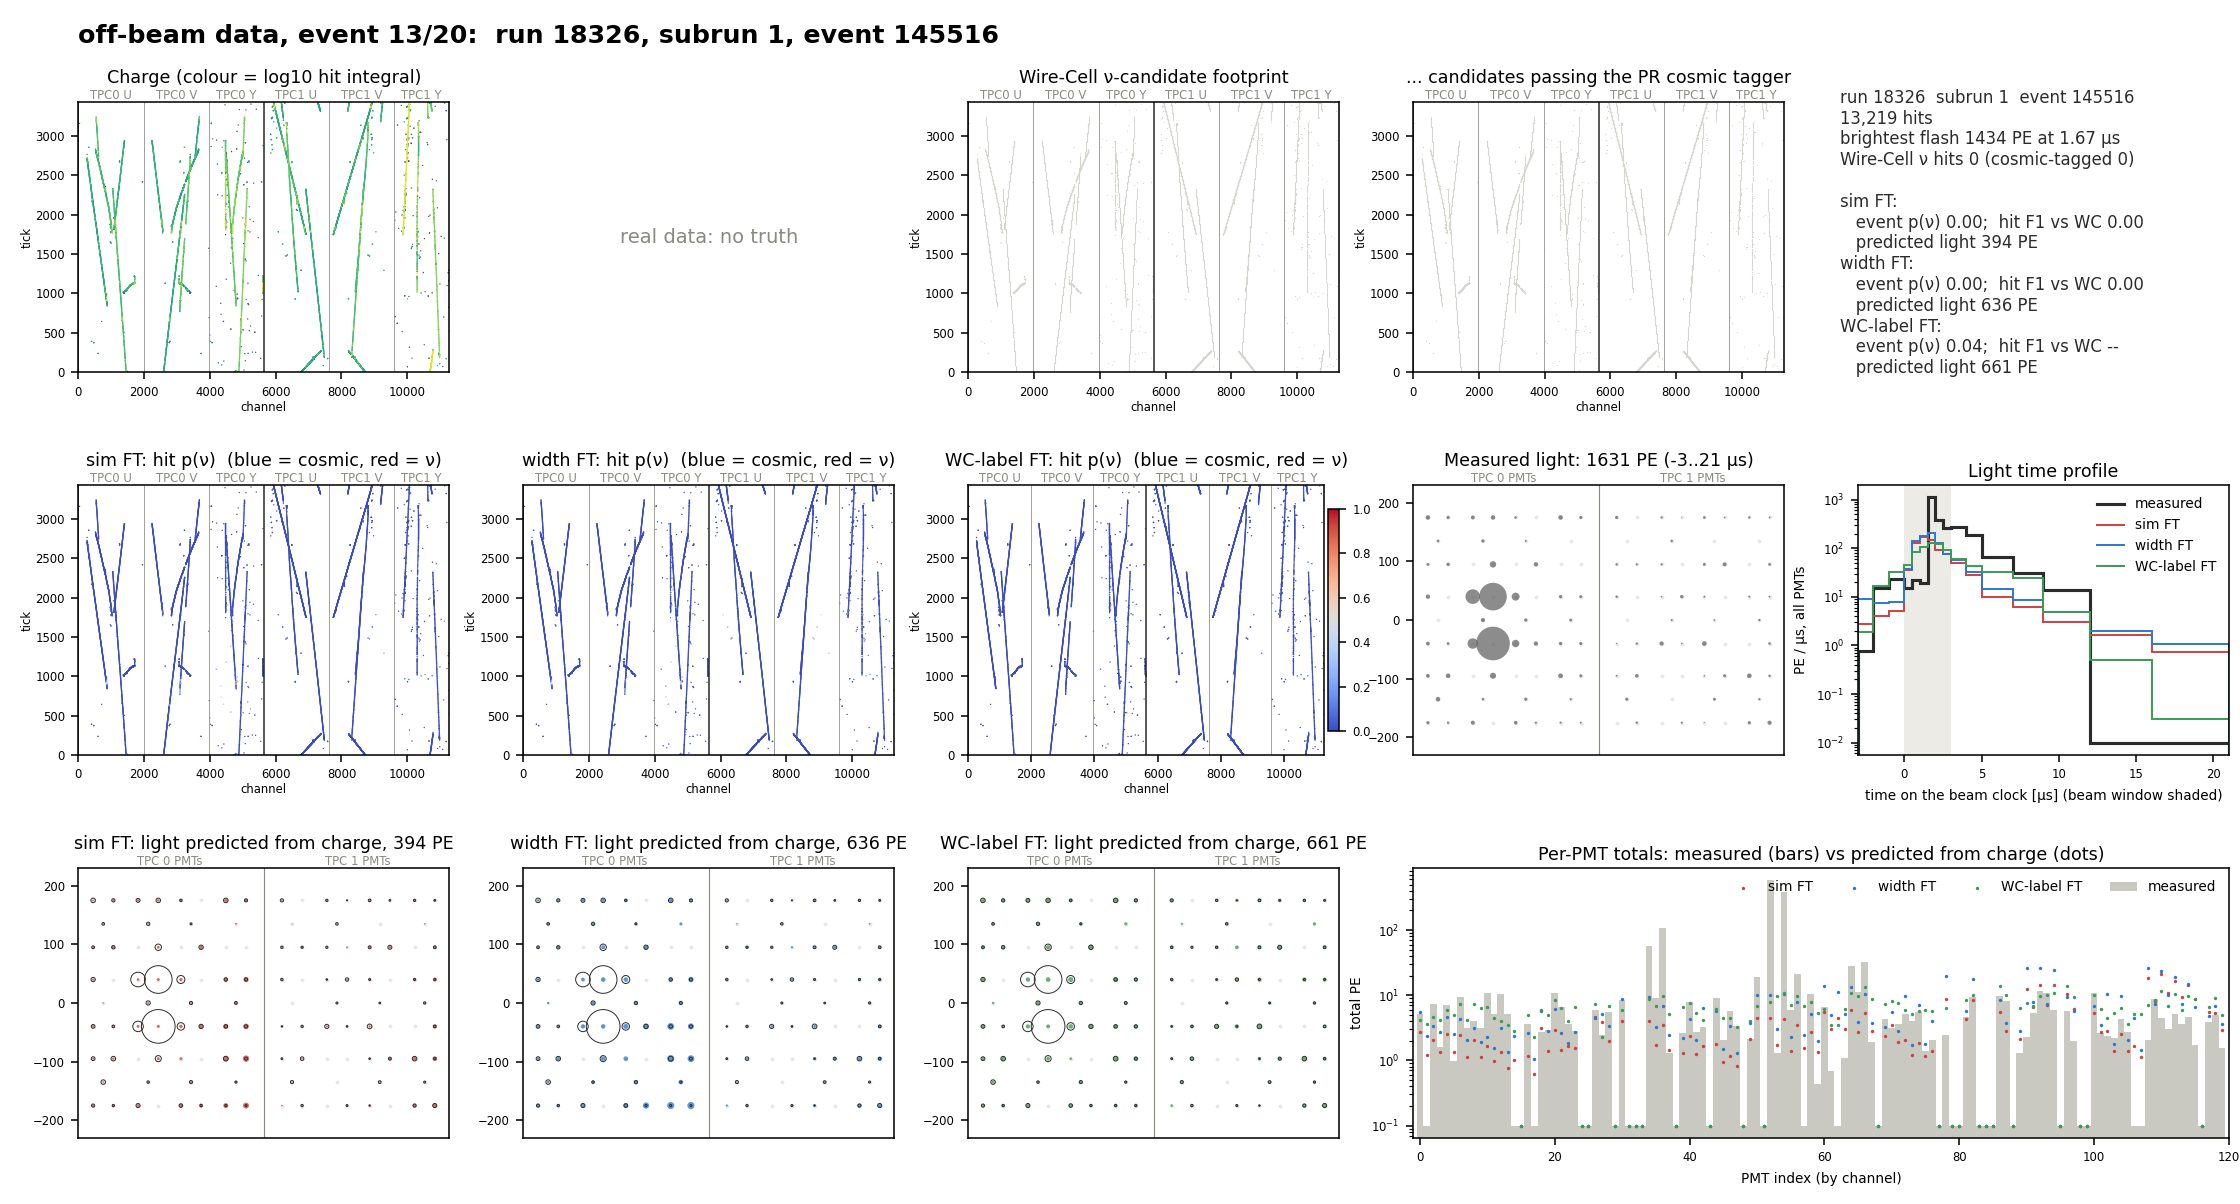
\includegraphics[width=\paperwidth,height=\paperheight,keepaspectratio]{displays/off_12.jpg}}
\end{frame}
% Off-beam data 14/20: run 18444, subrun 1, event 240124; event p(nu): sim FT 0.00, width FT 0.00, WC-label FT 0.16
\begin{frame}[plain]
  \centering\vspace*{-2pt}
  \makebox[\linewidth][c]{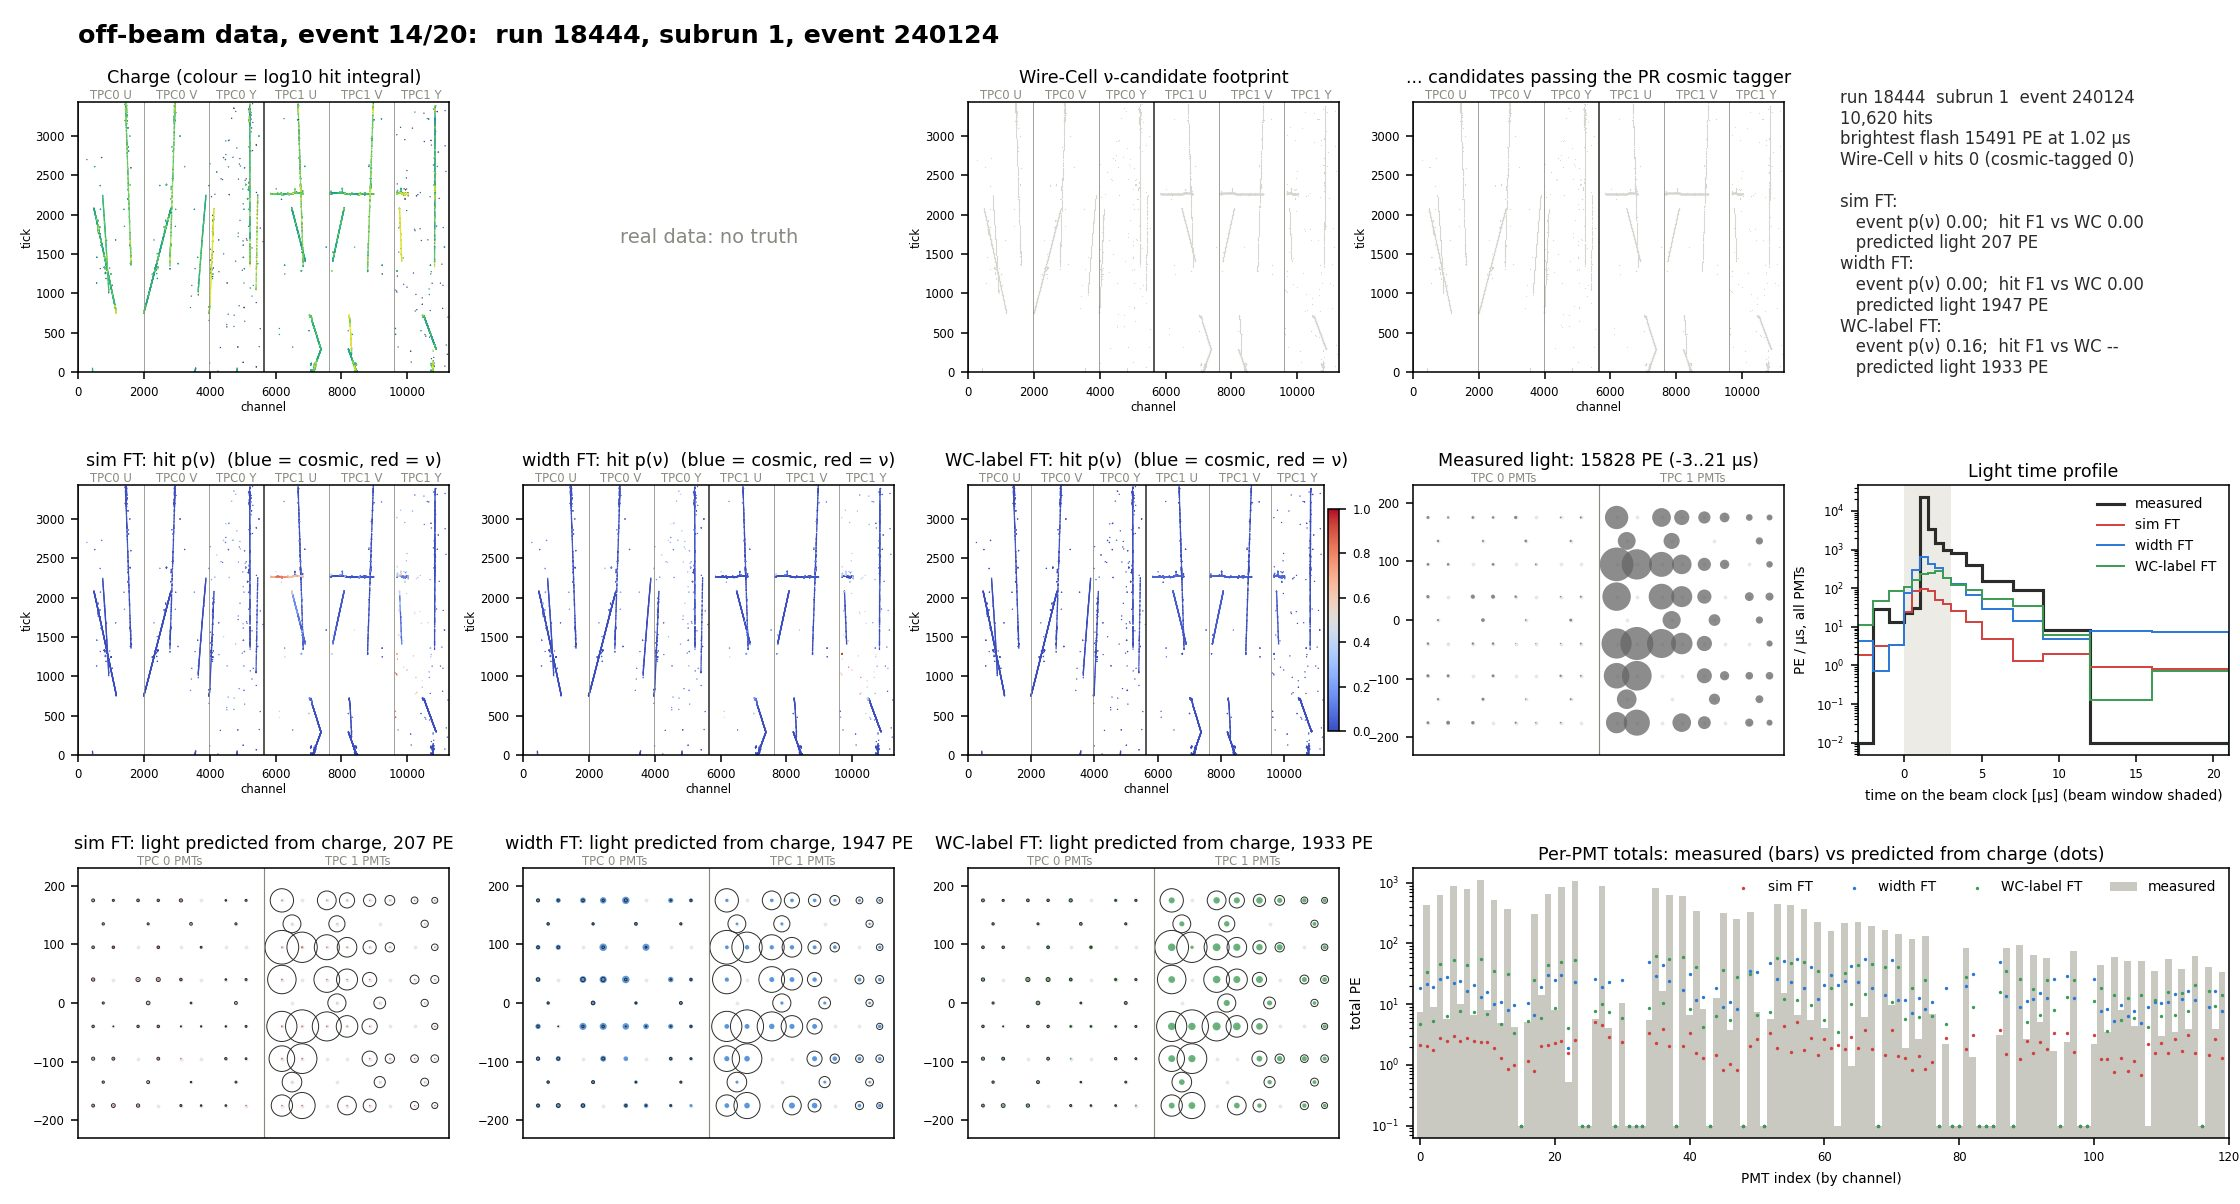
\includegraphics[width=\paperwidth,height=\paperheight,keepaspectratio]{displays/off_13.jpg}}
\end{frame}
% Off-beam data 15/20: run 18453, subrun 1, event 94673; event p(nu): sim FT 0.35, width FT 1.00, WC-label FT 0.15
\begin{frame}[plain]
  \centering\vspace*{-2pt}
  \makebox[\linewidth][c]{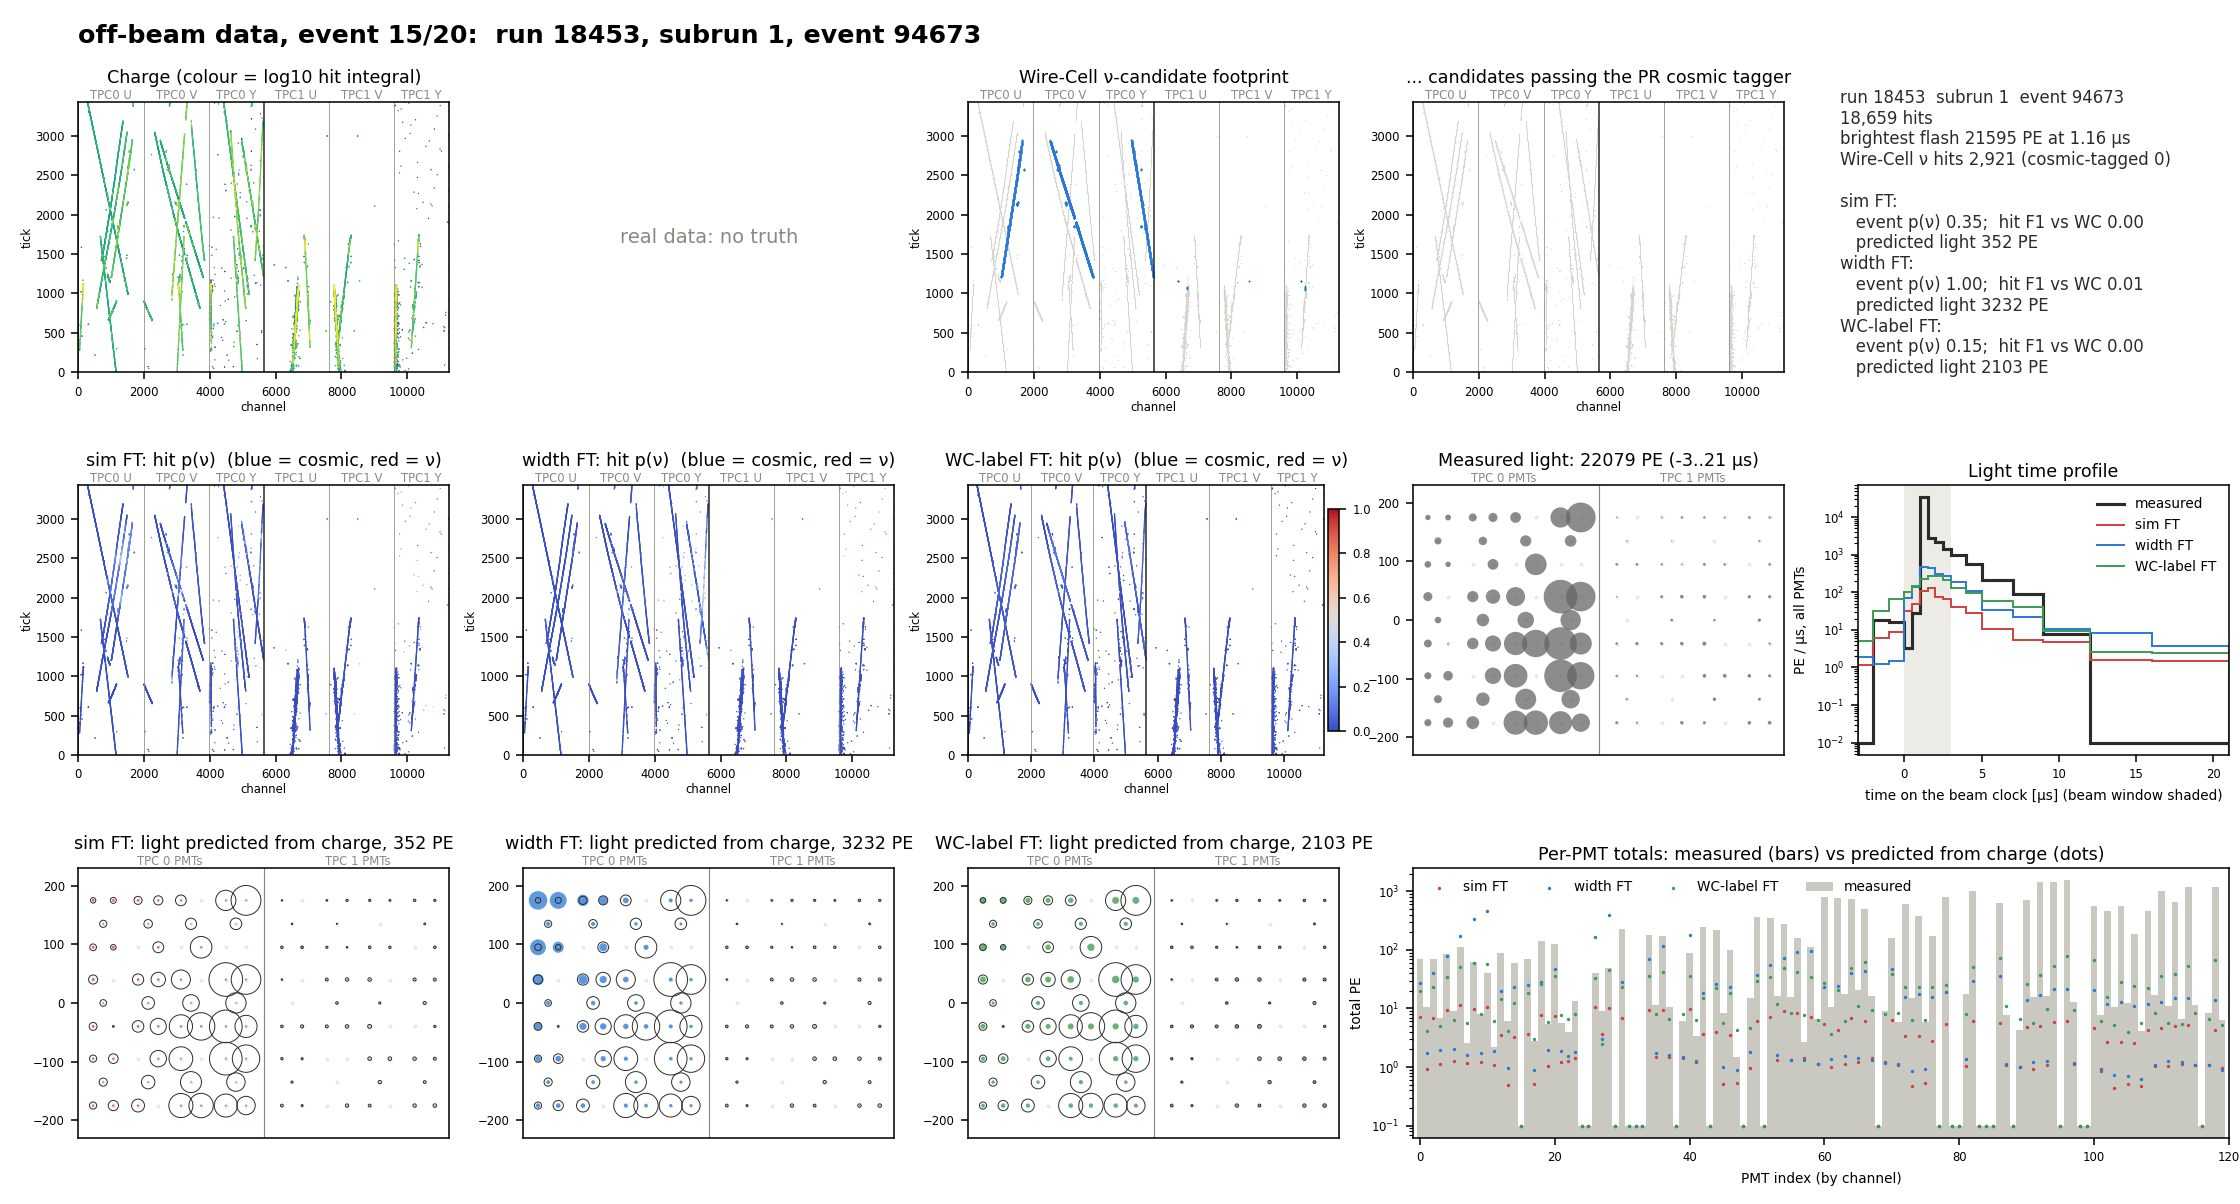
\includegraphics[width=\paperwidth,height=\paperheight,keepaspectratio]{displays/off_14.jpg}}
\end{frame}
% Off-beam data 16/20: run 18485, subrun 1, event 226962; event p(nu): sim FT 0.00, width FT 0.00, WC-label FT 0.01
\begin{frame}[plain]
  \centering\vspace*{-2pt}
  \makebox[\linewidth][c]{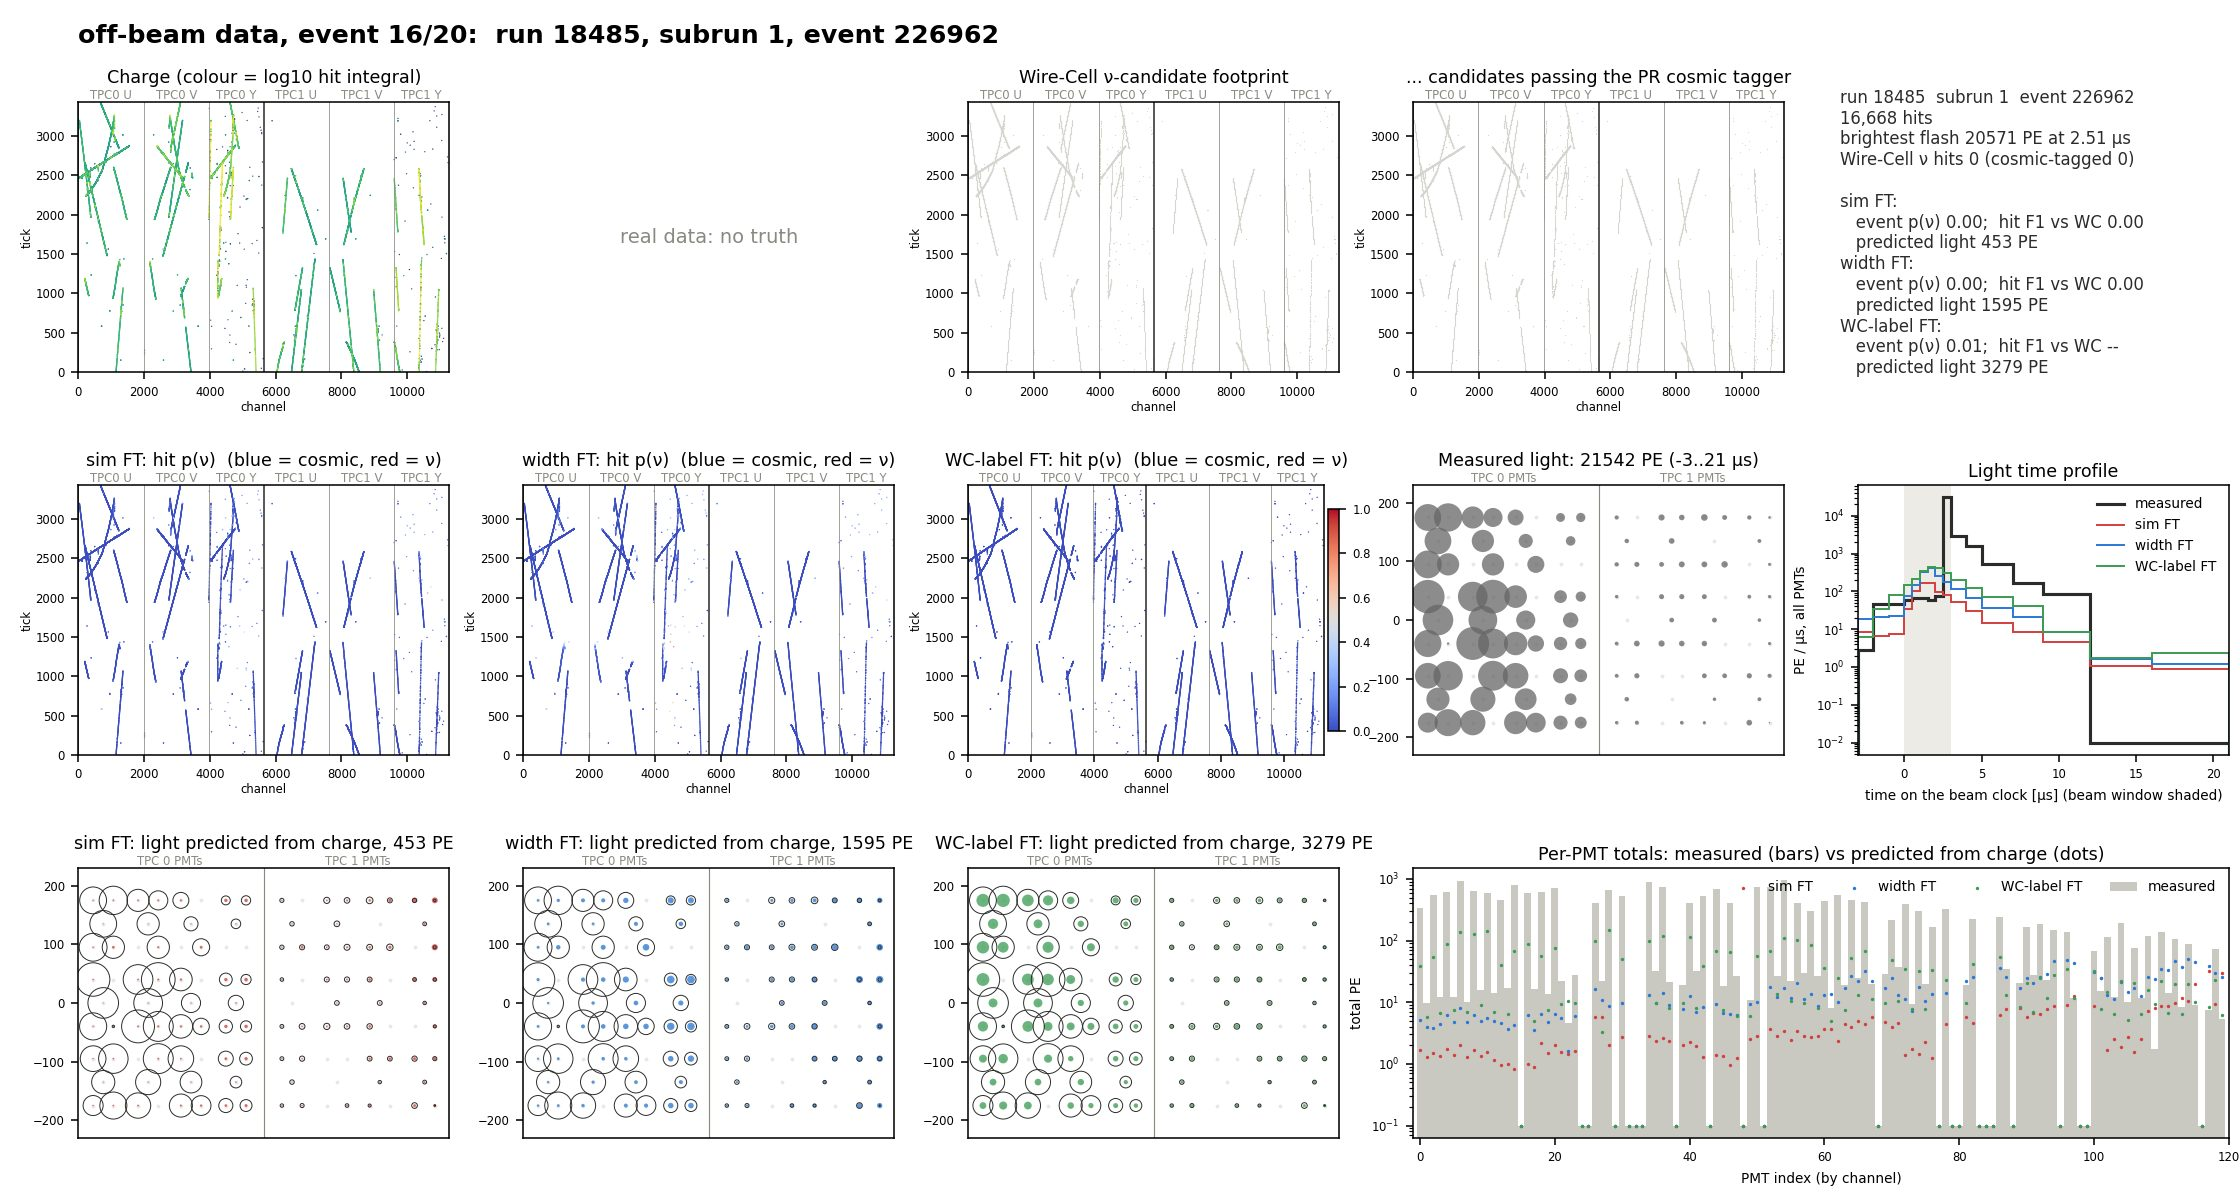
\includegraphics[width=\paperwidth,height=\paperheight,keepaspectratio]{displays/off_15.jpg}}
\end{frame}
% Off-beam data 17/20: run 18576, subrun 1, event 123870; event p(nu): sim FT 1.00, width FT 0.00, WC-label FT 0.29
\begin{frame}[plain]
  \centering\vspace*{-2pt}
  \makebox[\linewidth][c]{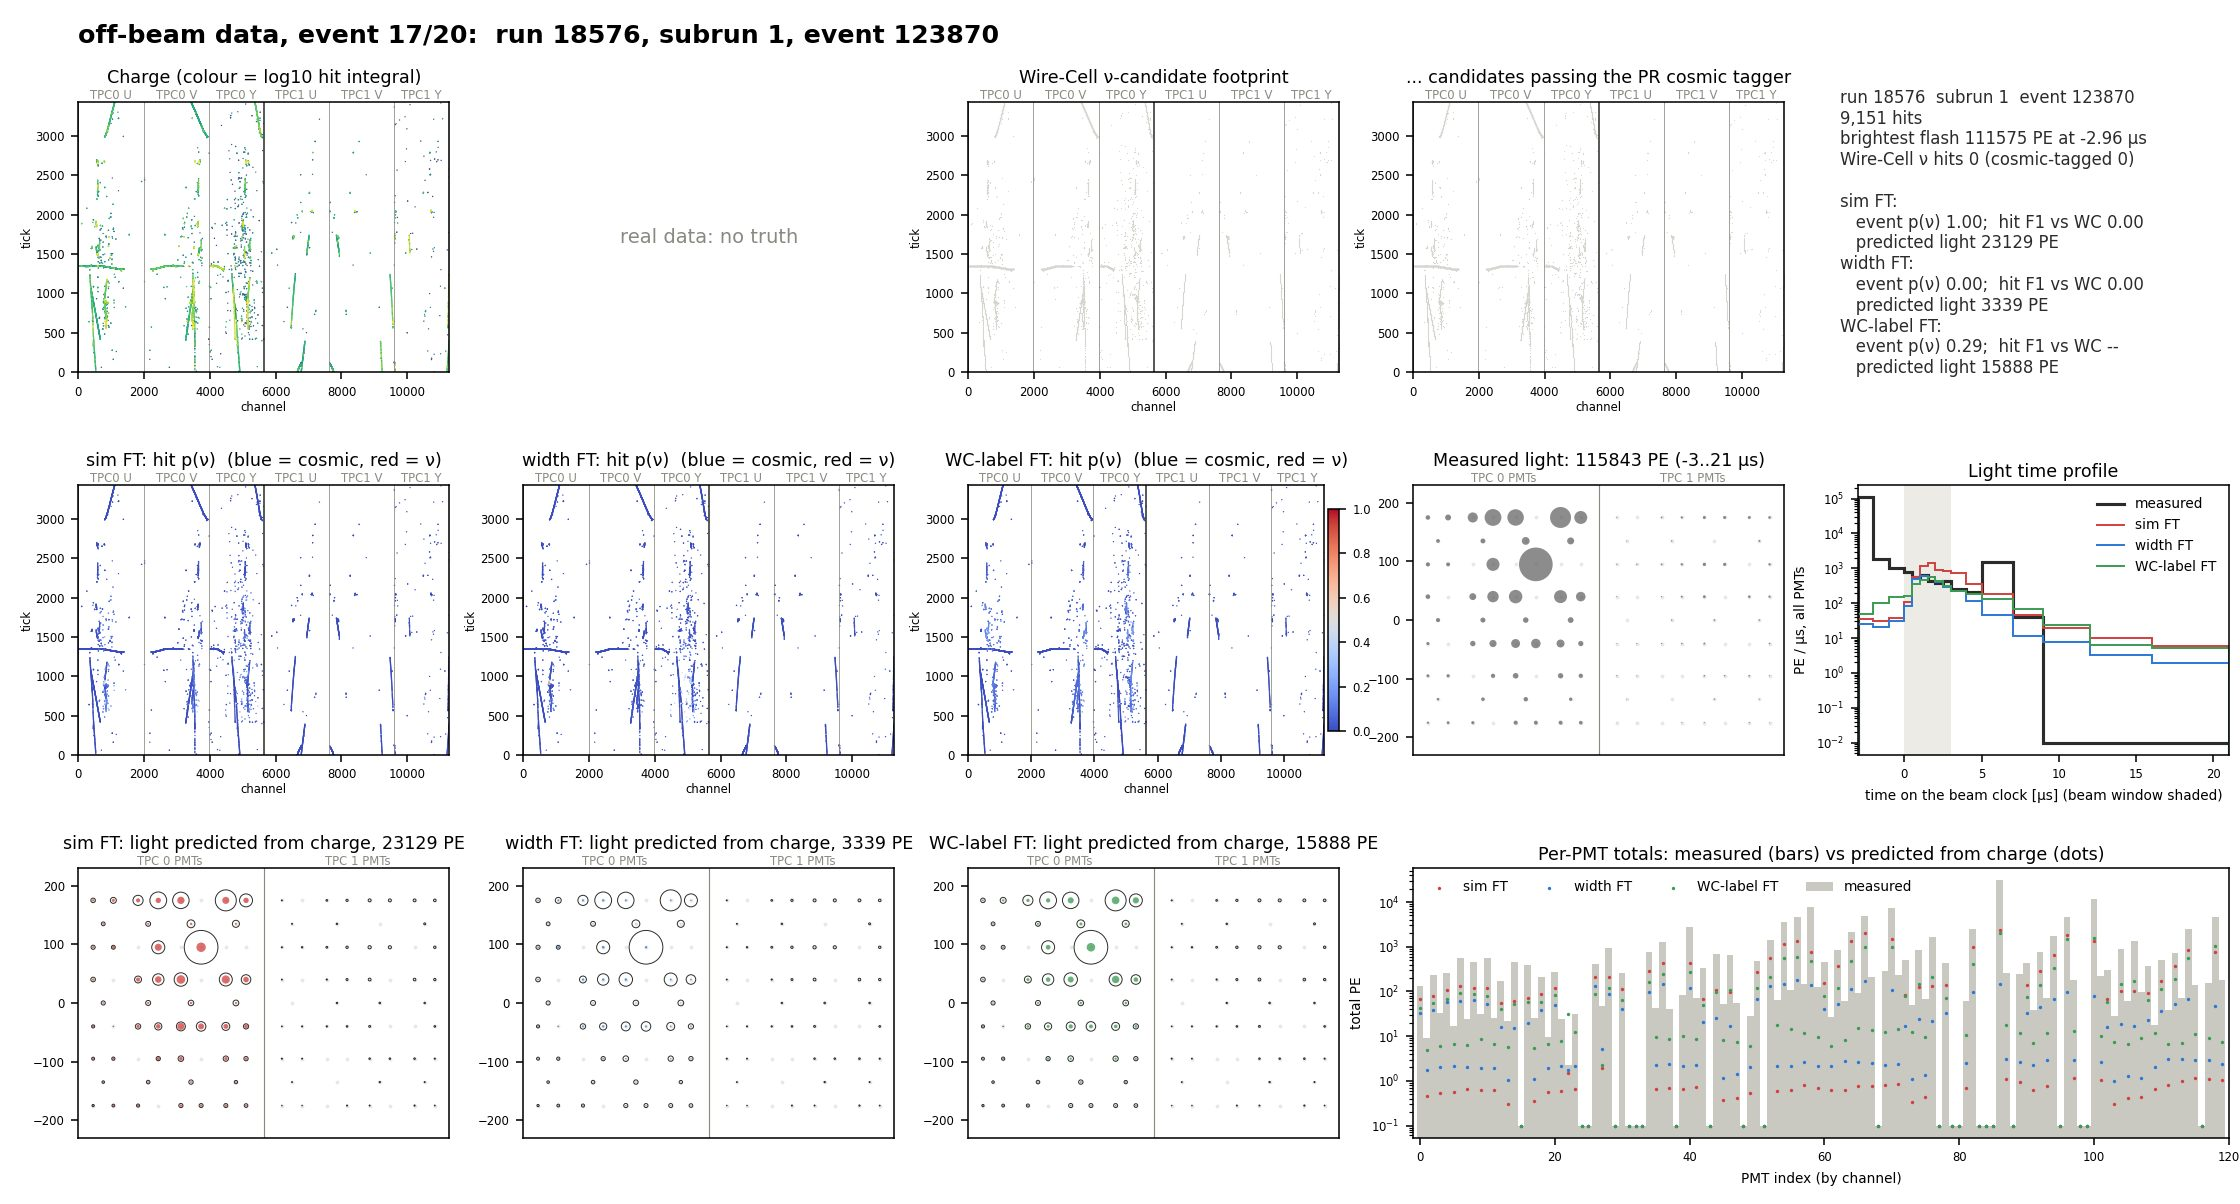
\includegraphics[width=\paperwidth,height=\paperheight,keepaspectratio]{displays/off_16.jpg}}
\end{frame}
% Off-beam data 18/20: run 18503, subrun 1, event 984786; event p(nu): sim FT 0.99, width FT 1.00, WC-label FT 0.08
\begin{frame}[plain]
  \centering\vspace*{-2pt}
  \makebox[\linewidth][c]{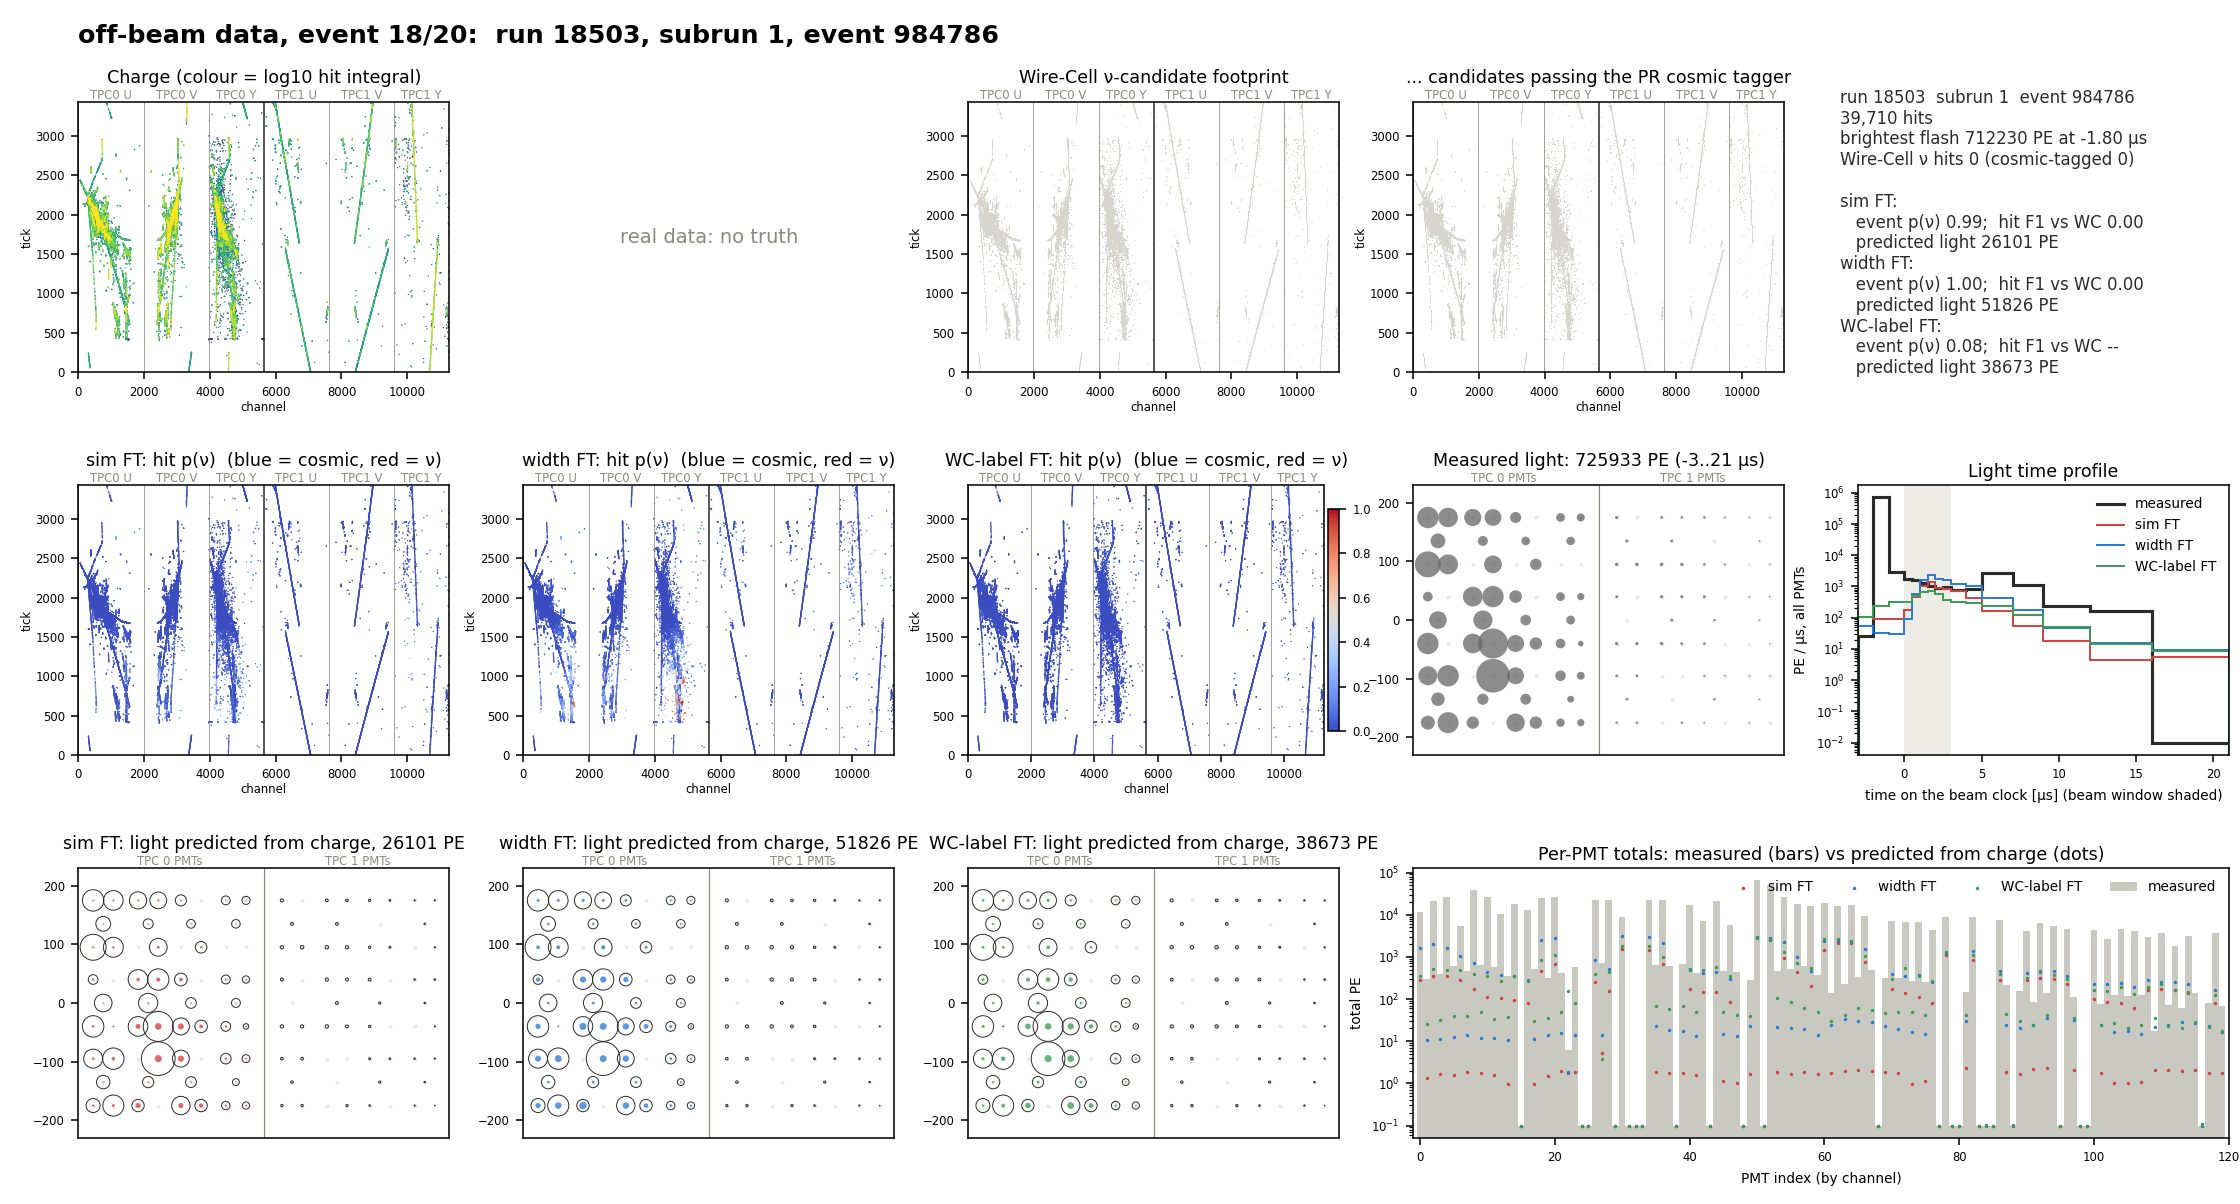
\includegraphics[width=\paperwidth,height=\paperheight,keepaspectratio]{displays/off_17.jpg}}
\end{frame}
% Off-beam data 19/20: run 18504, subrun 1, event 707279; event p(nu): sim FT 0.00, width FT 0.00, WC-label FT 0.02
\begin{frame}[plain]
  \centering\vspace*{-2pt}
  \makebox[\linewidth][c]{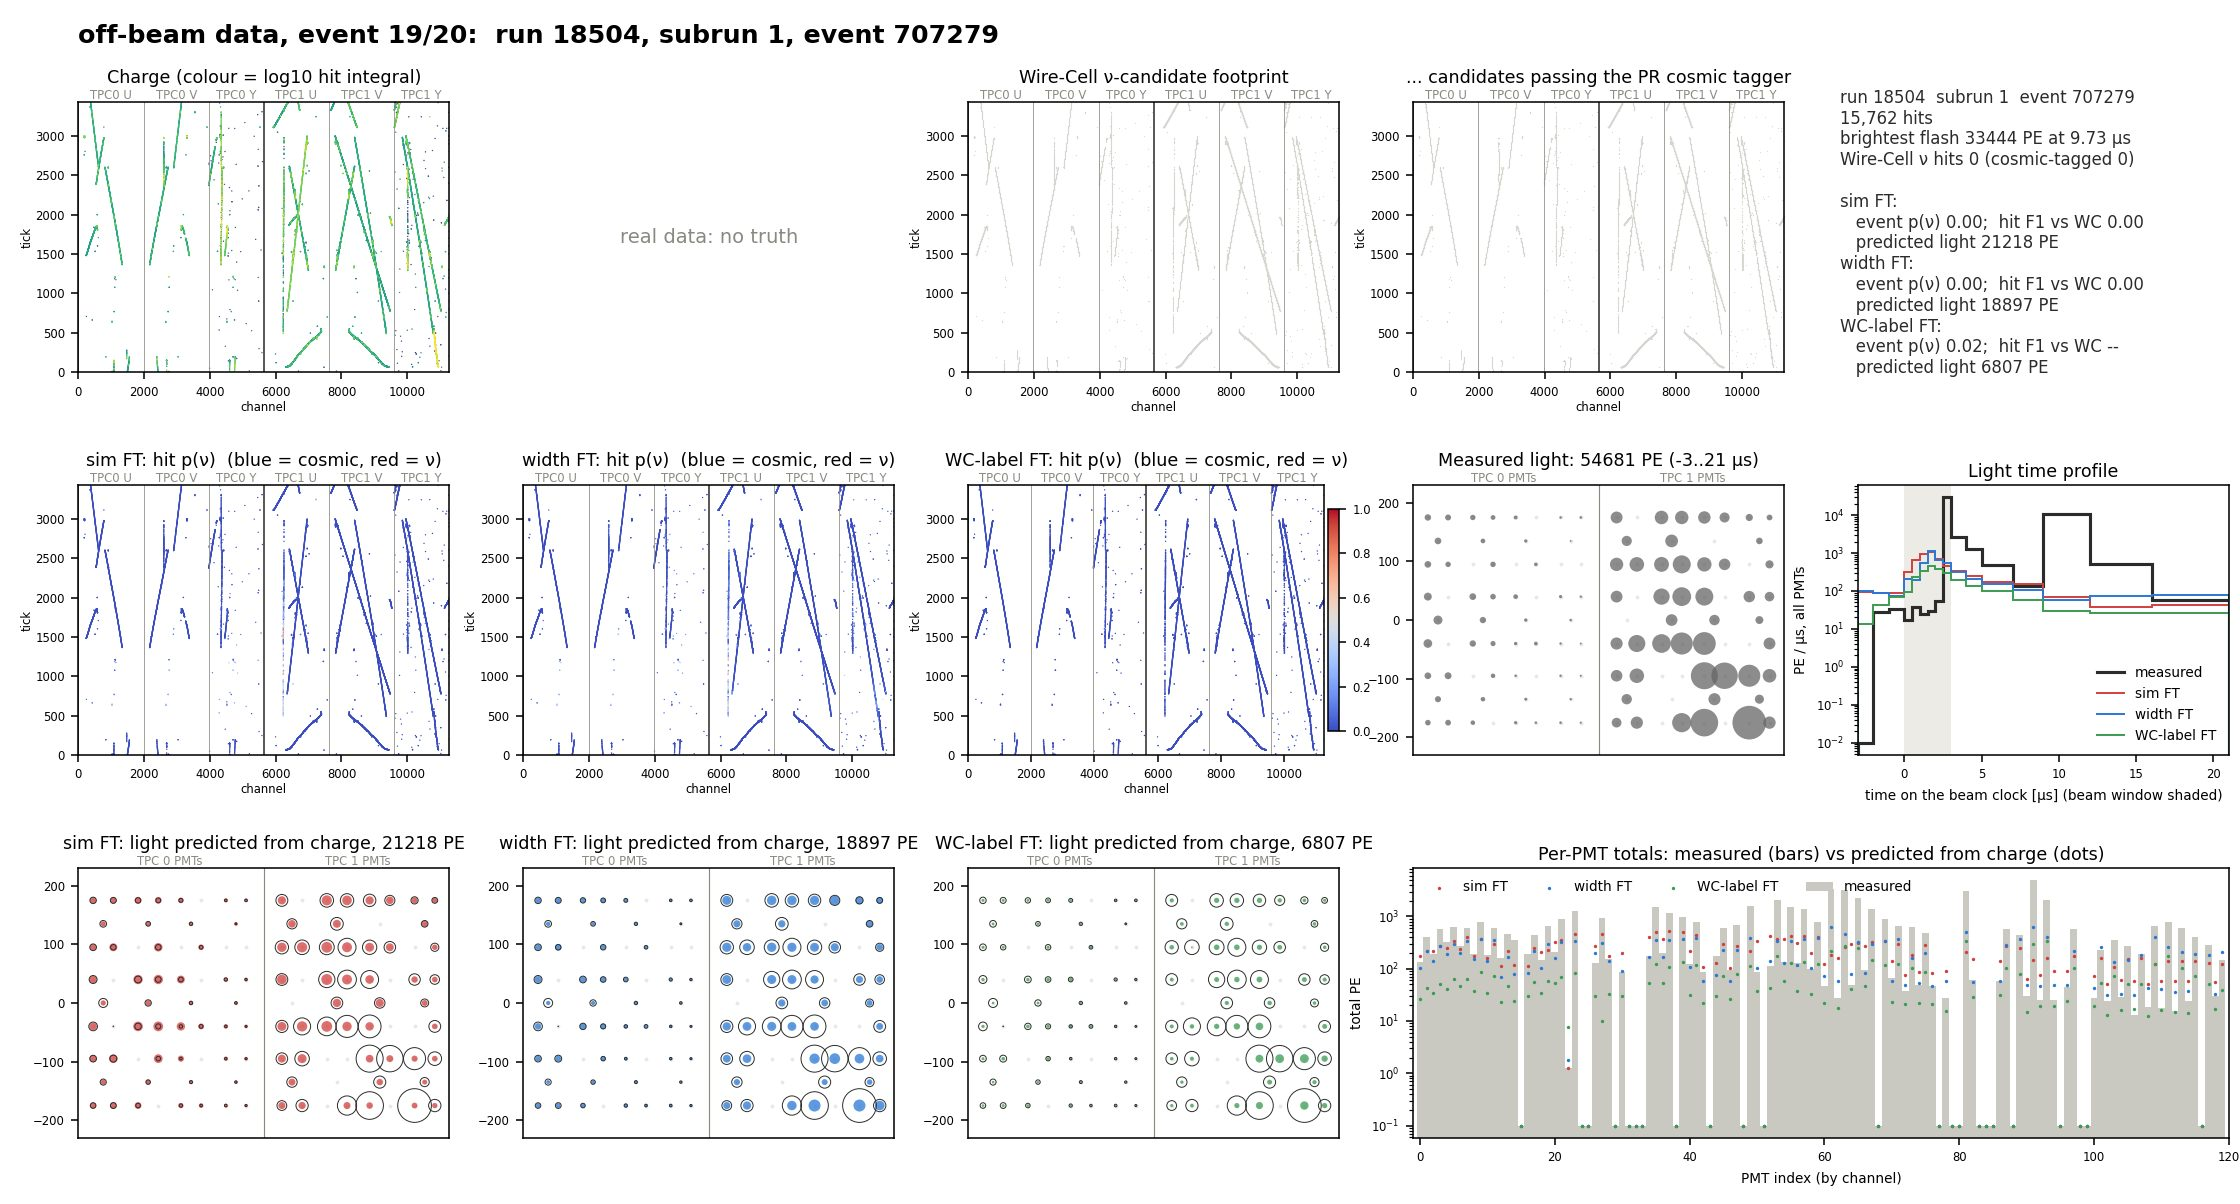
\includegraphics[width=\paperwidth,height=\paperheight,keepaspectratio]{displays/off_18.jpg}}
\end{frame}
% Off-beam data 20/20: run 18388, subrun 1, event 321351; event p(nu): sim FT 0.00, width FT 0.00, WC-label FT 0.04
\begin{frame}[plain]
  \centering\vspace*{-2pt}
  \makebox[\linewidth][c]{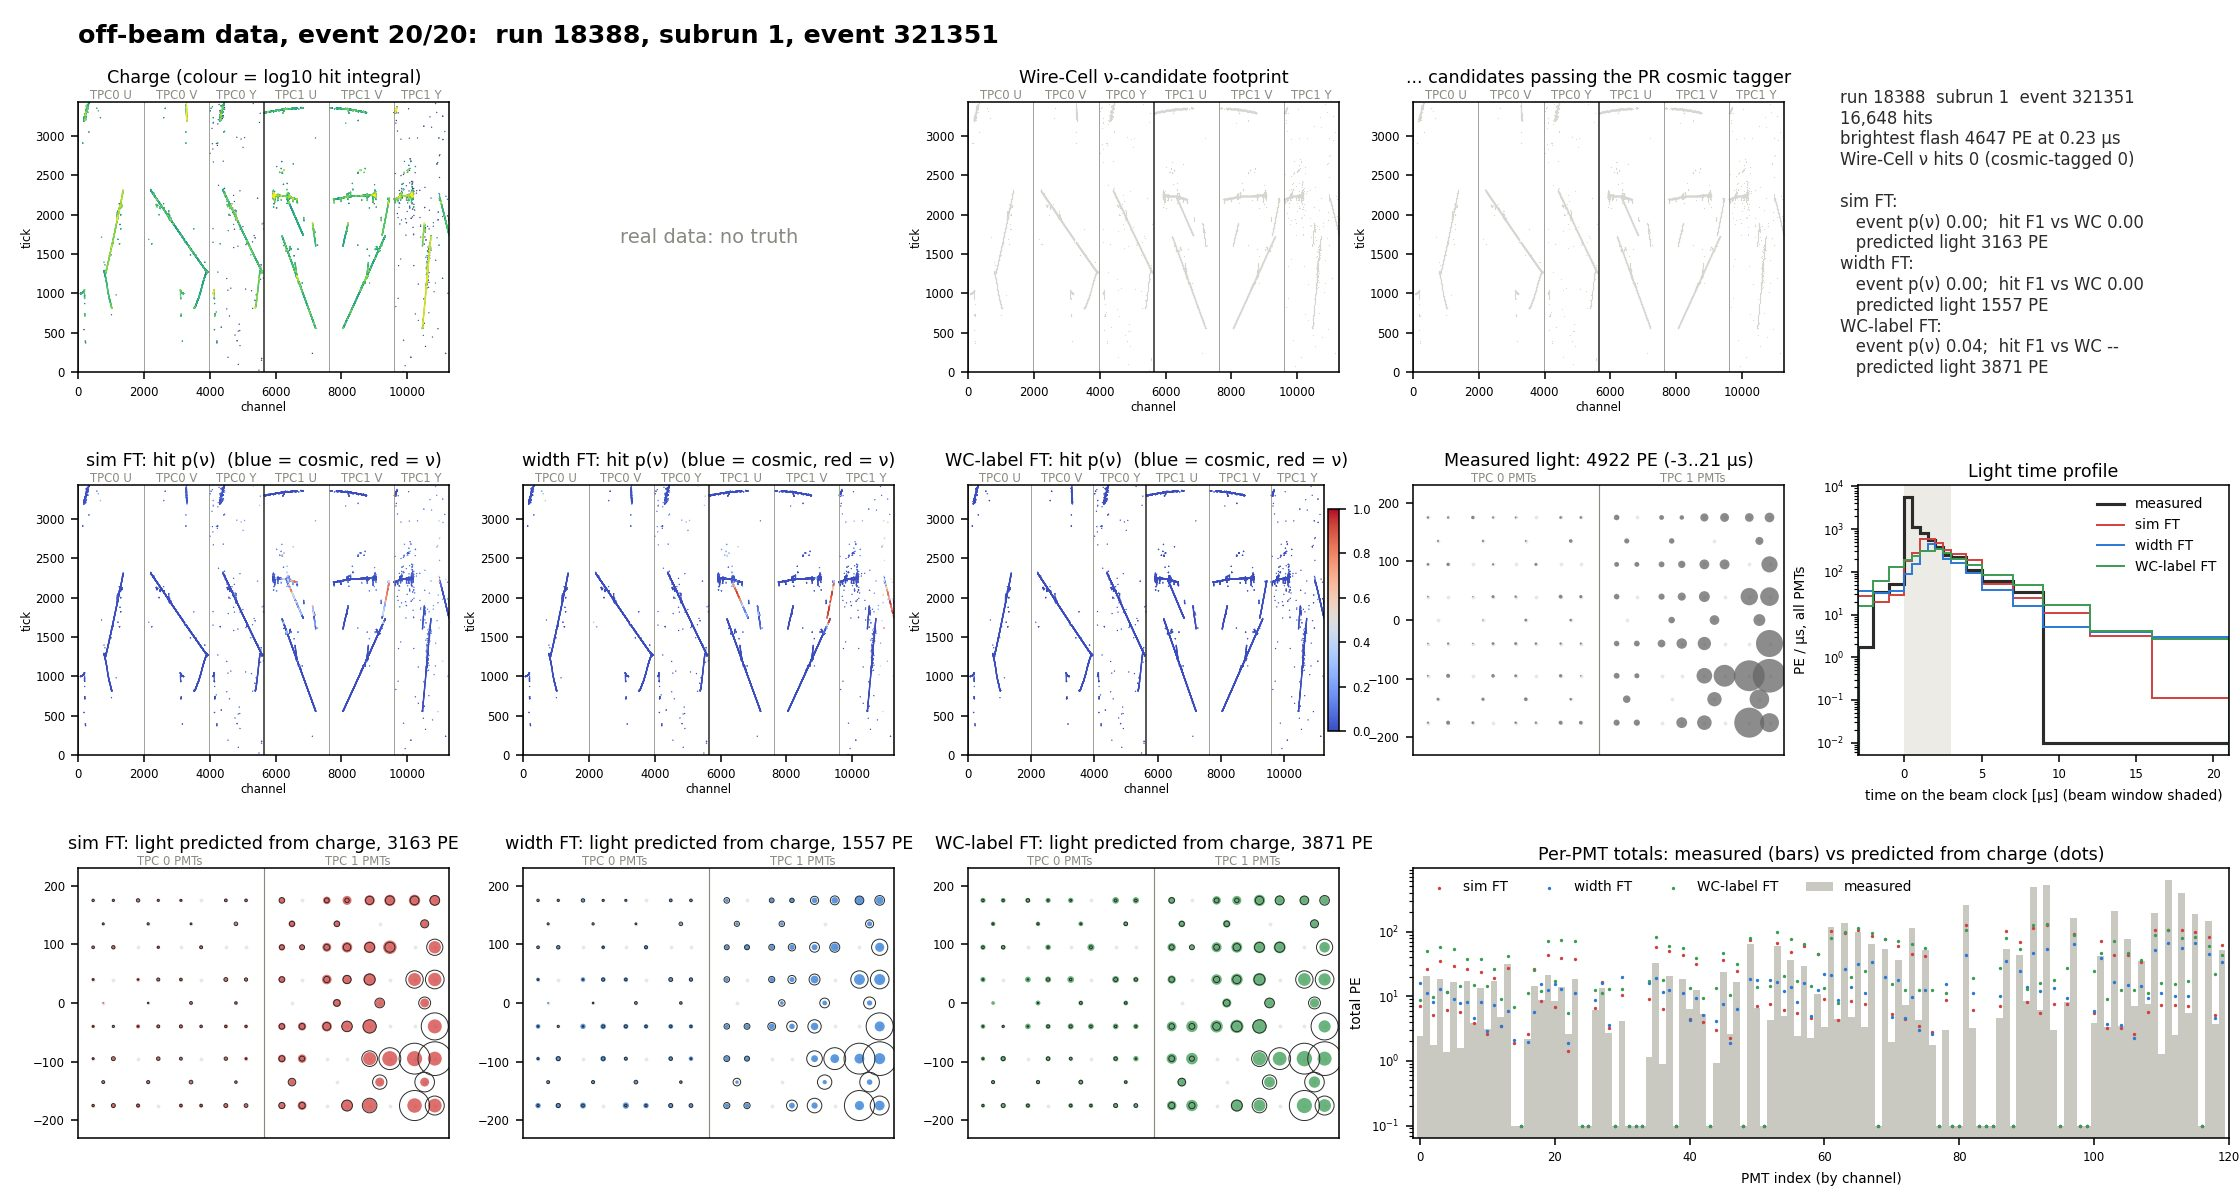
\includegraphics[width=\paperwidth,height=\paperheight,keepaspectratio]{displays/off_19.jpg}}
\end{frame}
